\documentclass{wzuthesis} % 不填充空白页。如果需要双面打印版，请注释掉本行并启用下一行
% \documentclass[print-both-sides]{scutthesis} % 使用双面打印版（填充额外空白页以保证每一章开头都在奇数页）
\usepackage{mathptmx}
% Note: enumitem, booktabs, graphicx, subcaption, caption, hyperref already loaded by wzuthesis.cls
\usepackage{bicaption}
\usepackage{amsmath}
\usepackage{amssymb}
\usepackage{algorithm}
\usepackage{algpseudocode}
\usepackage{float}
\usepackage{rotating} % for sidewaystable in SBO chapter

\bicaptionsetup[figure]{}{name=Fig.}
\bicaptionsetup[table]{}{name=Table}
\setlength{\headheight}{13pt}

% Algorithm helper commands (from BEXEA)
\newcommand{\Indent}{\State\hspace{\algorithmicindent}}
\newcommand{\Indentx}{\Statex\hspace{\algorithmicindent}}

\setmainfont{Times New Roman}[
UprightFont = *,
BoldFont = * Bold,
ItalicFont = * Italic,
BoldItalicFont = * Bold Italic
]

%%===============论文信息=============================
\ctitle{改进元启发式算法及其在特征选择与昂贵优化中的应用研究}
                                % 中文题目
\etitle{Research on Improved Metaheuristic Algorithms and Their Applications in Feature Selection and Expensive Optimization}                     % 英文题目

\cauthor{王\ 健}            % 作者姓名
\fen{TP18}                  % 分类号
\udc{004.8}                    % UDC
\id{23451350032}               % 学号
\mi{公开}                       % 密级
\xwlx{学术型}                   %学位类型
\pylx{全日制统招研究生}         % 培养类型
\cmajor{计算机科学与技术}       % 专业名称
\cclass{计算机软件与理论}              % 研究方向
\cmentor{陈慧灵（教授）} % 指导老师
\cdata{2025年3月1日} %完成时间
\blindcode{} % 盲审代码
%%===================================================
% \def\blind{}       % 盲审版把这条注释打开



\cabstract{
元启发式算法因其无需梯度信息即可求解复杂优化问题的特性，在工程设计、机器学习和科学计算等领域得到广泛应用。然而，现有算法在探索与利用平衡、搜索策略自适应以及昂贵优化场景下的样本效率等方面仍存在不足。本文围绕元启发式优化算法的改进与应用展开研究，提出了三种新型算法，并在多个实际应用场景中验证了其有效性。主要研究工作如下：

（1）针对回溯搜索算法（BSA）固有随机性导致的探索与利用失衡问题，提出了基于精英引导变异策略的改进回溯搜索算法（IBSA）。通过改进变异和交叉算子以充分利用精英个体信息，增强了算法在最优区域附近的局部搜索精度。在IEEE CEC 2017基准函数上与23种先进算法进行对比实验，结果表明IBSA在收敛速度和求解精度方面均优于原始BSA。进一步开发了二值版本bIBSA，将其应用于12个医学数据集的特征选择任务，实验结果验证了bIBSA在二值优化领域的优越性能。

（2）受人类社会地位追求行为启发，提出了一种新型元启发式算法——基于状态的优化算法（SBO）。SBO模拟个体向高地位人物靠拢、学习和获取资源的社会行为模式，将其转化为高效的计算优化方法。在IEEE CEC 2017测试套件的10、30、50和100维问题上进行了全面对比分析。此外，SBO在9个高维数据集的特征选择任务中表现出色，在3阈值水平的乳腺癌组织学图像多阈值分割应用中也展现了优异的性能。

（3）针对昂贵优化问题中现有代理辅助进化算法搜索策略固定、不确定性准则可解释性不足的问题，提出了基于赌博机驱动的自适应搜索代理辅助进化算法（BEXEA）。引入多臂赌博机机制，通过强化学习根据环境反馈自主调整搜索模式，实现探索与利用的动态平衡；同时提出可解释的不确定性准则，将特征差异熵融入期望改进（EI）准则，提升代理模型精度。在两组复杂基准测试集和油藏产量优化实际问题上的数值实验表明，BEXEA优于七种先进的代理辅助进化算法。
}
\ckeywords{元启发式算法, 回溯搜索算法, 特征选择, 代理辅助优化, 多臂赌博机}

\eabstract{
Metaheuristic algorithms have been widely applied in engineering design, machine learning, and scientific computing due to their ability to solve complex optimization problems without requiring gradient information. However, existing algorithms still face challenges in balancing exploration and exploitation, achieving adaptive search strategy selection, and improving sample efficiency in expensive optimization scenarios. This thesis focuses on the improvement and application of metaheuristic optimization algorithms, proposing three novel algorithms and validating their effectiveness across multiple practical application scenarios. The main contributions are as follows:

(1) To address the imbalance between exploration and exploitation caused by the inherent randomness in the Backtracking Search Algorithm (BSA), an Improved Backtracking Search Algorithm (IBSA) with an elite leading mutation strategy is proposed. By modifying the mutation and crossover operators to better utilize elite individual information, the algorithm enhances local search accuracy near optimal regions. Comparative experiments against 23 state-of-the-art algorithms on the IEEE CEC 2017 benchmark functions demonstrate that IBSA outperforms the original BSA in both convergence speed and solution accuracy. A binary version, bIBSA, is further developed and applied to feature selection tasks on 12 medical datasets, confirming its superior performance in the binary optimization domain.

(2) Inspired by the human desire for status advancement, a novel metaheuristic algorithm called Status-based Optimization (SBO) is proposed. SBO emulates how individuals seek proximity to, learn from, and acquire resources from high-status figures, translating these social behavioral patterns into an efficient computational optimization method. Comprehensive comparative analyses are conducted on the IEEE CEC 2017 test suite across problem dimensions of 10, 30, 50, and 100. Furthermore, SBO excels in feature selection tasks on 9 high-dimensional datasets and demonstrates outstanding performance in multi-threshold image segmentation of breast cancer histology images at 3 threshold levels.

(3) To overcome the limitations of fixed search strategies and insufficient interpretability of uncertainty criteria in existing surrogate-assisted evolutionary algorithms (SAEAs) for expensive optimization problems, a Bandit-driven Explainable Evolutionary Algorithm (BEXEA) is proposed. A multi-armed bandit mechanism is introduced to autonomously adjust the search mode based on environmental feedback through reinforcement learning, achieving dynamic balance between exploration and exploitation. Meanwhile, an explainable uncertainty criterion is proposed by incorporating the entropy of feature differences into the Expected Improvement (EI) criterion to enhance surrogate model accuracy. Numerical experiments on two complex benchmark sets and a real-world oil reservoir production optimization problem demonstrate the superiority of BEXEA over seven state-of-the-art SAEAs.
}
% 英文文关键词(每个关键词之间用,分开, 最后一个关键词不打标点符号。)
\ekeywords{metaheuristic algorithm, backtracking search algorithm, feature selection, surrogate-assisted optimization, multi-armed bandit}

\begin{document}
% 论文前置部分
\frontmatter
\makefirstpage
% 如果不需要图、表目录前往cls文件中将相应的注释掉

% 论文主体部分
\mainmatter

%%% Chapter 1: 绪论 (Introduction)
% Chapter 1: 绪论 (Introduction)
\chapter{绪论}

\section{研究背景和意义}

现实环境中的优化任务正面临高维、非线性及多模态等复杂挑战，这类NP-hard问题广泛存在于工程设计\cite{ibsa_ref1}、机器学习超参调优\cite{ibsa_ref3}以及生物信息学\cite{ibsa_ref15}等领域。面对庞杂的搜索空间，传统确定性算法过度依赖梯度信息，往往难以稳定地捕获全局最优解\cite{ibsa_ref4}。与此同时，互联网技术的普及引发了数据规模的爆发式增长，高维复杂数据渗透进医疗诊断\cite{ibsa_ref11}、路径规划\cite{ibsa_ref9}和金融服务\cite{ibsa_ref8}等各行各业。这类数据通常夹杂着大量冗余或无效信息，不仅加剧了存储与计算负担，还会干扰学习模型的表征能力，削弱预测精度\cite{ibsa_ref17}。

元启发式算法通过模拟自然界的生物演化、群体协同或物理规律进行随机寻优，凭借其无梯度依赖、部署灵活及全局搜索能力较强等优势，已成为求解复杂优化问题的有效方法\cite{ibsa_ref16}，在特征选择\cite{ibsa_ref50}、图像多阈值分割\cite{ibsa_ref45}及调度优化\cite{ibsa_ref48}等任务中均有广泛应用。例如，Harris Hawks算法在处理工程约束问题时表现出优异的收敛性\cite{ibsa_ref83}；黏菌算法则在多模态景观搜索中具备良好的鲁棒性\cite{ibsa_ref28}。这些工作不仅丰富了计算智能理论，也为解决实际工程痛点提供了可行路径。

尽管元启发式算法展现出巨大潜力，但现有研究仍面临若干瓶颈。首要挑战在于探索与开发行为的失衡\cite{ibsa_ref75}，这常导致搜索前期覆盖不足或后期陷入局部极值。以高维医学数据特征选择为例，指数级增长的搜索空间要求算法在维持诊断性能的同时，必须精准剔除冗余特征，否则会显著加重分类器的计算负担。其次，搜索策略的选择及参数设置往往过度依赖人工先验经验\cite{ibsa_ref65}，削弱了算法应对多变问题的适应力。例如在多阈值图像分割任务中，噪声干扰、灰度不均等因素使得搜索景观差异巨大，静态机制难以维持性能的一致性。此外，在计算昂贵优化场景下，真实评估成本极高，样本利用效率直接制约了优化成效\cite{he2023review}。如油藏产量优化、翼型设计等工程问题，单次评估往往涉及复杂的数值模拟，如果采样缺乏导向性，有限的计算资源将迅速枯竭。针对上述难题，本研究从精英信息挖掘、自适应策略调控及代理模型辅助等方面切入，探索元启发式算法的演化机理与应用路径。

从应用维度审视，高维特征选择、医学影像分割与昂贵工程优化虽形式各异，其核心诉求均指向了有限计算资源下的高效寻优。特征选择侧重于在离散空间压缩维度，力求提升模型的可解释性与诊断精度\cite{ibsa_ref50}；多阈值分割则需在连续灰度域内精准定位，直接关系到病灶提取的可靠性\cite{sbo_ref82,sbo_ref83}；而昂贵优化更强调每一次评估的实际价值，力求以最小的计算成本换取最优的决策方案\cite{liu2023airfoils,kumar2024optimization}。这三类场景精准对接了探索与开发平衡、策略自适应与样本效率提升这三大核心瓶颈，为本研究提供了典型应用场景。

研究复杂优化环境下的元启发式改进策略，兼具理论深度与工程价值。在理论层面，这有助于解析搜索行为的演化规律，完善多样性维持与自适应决策机制\cite{ibsa_ref75}。在应用层面，高效的寻优算法能显著降低实际生产中的计算开销。通过在医学特征选择中降低特征冗余度，可以增强辅助诊断的稳健性；在图像分割任务中，能够提升病灶边缘识别的精细度；而在昂贵工程设计中，则能大幅缩短设计周期，确保参数决策的科学性\cite{ibsa_ref49,sbo_ref79,kudela2022recent}。

\section{国内外研究现状}

\subsection{元启发式优化算法研究现状}

元启发式算法在求解复杂优化问题中表现出独特优势，其灵感源于对自然界生物行为或物理规律的工程模拟。按机制差异可将其划分为生物启发（如PSO\cite{ibsa_ref26}、GWO\cite{ibsa_ref81}）、进化计算（如GA\cite{ibsa_ref33}、DE\cite{ibsa_ref34}）、物理化学过程模拟（如SA\cite{ibsa_ref29}、EO\cite{ibsa_ref32}）以及人类行为模仿（如TLBO\cite{ibsa_ref37}、BSO\cite{ibsa_ref40}）等体系。近年来，HHO\cite{ibsa_ref83}、SCA\cite{ibsa_ref31}及RIME\cite{sbo_ref49}等新型算法相继问世，进一步拓宽了该领域的研究范畴。

目前的改进研究主要聚焦于自适应参数控制、异构策略融合及种群多样性维系，旨在提升算法的收敛速度与跨场景稳定性。Li等人\cite{ibsa_ref76}通过多策略增强显著提升了北苍鹰算法的工程应用性能；Nadimi-Shahraki等人\cite{ibsa_ref88}对灰狼优化器进行了机制改进，强化了其求解复杂约束问题的能力；Nenavath与Jatoth\cite{ibsa_ref87}则通过融合正弦余弦算子与差分变异，在全局优化中取得了突破。针对BSA算法，Zhao等人\cite{ibsa_ref57}引入种群控制因子以增强搜索精度，Chen等人\cite{ibsa_ref63}则利用知识学习机制提升了其演化效率。

从近三年的进展来看，元启发式领域的研究重点正从单一算子开发转向跨场景验证与工程适用性提升。2023年出现的GWCA算法通过模拟长城修筑中的分工协作，提升了约束优化性能；WaOA算法则基于海象的集群行为构建了多阶段搜索框架\cite{gwca2023,waoa2023}。2024年，RBMO与SBOA算法相继被提出，分别借鉴红嘴蓝鹊的捕食协作与秘书鸟的防御机制设计了新型演化规则\cite{rbmo2024,sboa2024}。2025年，研究者开始关注复杂动态环境下的策略稳健性，如ASHSBOA通过自适应学习策略显著提升了三维路径规划的效率\cite{ashsboa2025}。

“无免费午餐”定理揭示了优化领域的本质：不存在适用于所有场景的通用算法\cite{sbo_ref95}。这一认识确立了针对特定任务定制化设计算法的必要性。尽管前人已取得丰硕成果，但探索开发失衡、对经验调参的路径依赖以及复杂环境下的稳定性瓶颈依然存在。特别是在处理高维特征选择、医学影像分割等实际应用时，算法性能往往出现大幅波动。如何设计具备较强环境适应能力与策略自适应性的改进方案，仍是计算智能领域的重要方向。

\subsection{特征选择方法研究现状}

在现代数据分析领域，海量高维数据带来了严峻的维度灾难挑战。这些数据中往往充斥着干扰项与重复信息，严重制约了模型的泛化能力\cite{ibsa_ref17,ibsa_ref18}。特征选择（Feature Selection, FS）作为降维的核心手段，通过提取最具判别力的特征子集，在简化模型结构的同时提升其解释力\cite{ibsa_ref50}。现有手段可归纳为过滤式、嵌入式与包裹式三类：过滤式侧重统计特征，计算效率高但忽略了特征间的复杂交互\cite{ibsa_ref20}；嵌入式深度耦合学习器\cite{ibsa_ref21}；而包裹式以分类精度为导向，虽然算力开销较大，但在特定任务下的表现通常更胜一筹\cite{ibsa_ref23}。

鉴于包裹式特征选择本质上属于离散组合优化，元启发式算法因其强大的搜索潜能而被广泛采用\cite{ibsa_ref95}。Mafarja等人\cite{ibsa_ref51}探索了鲸鱼优化在特征选择中的应用；Abdel-Basset等人\cite{ibsa_ref42}通过融合模拟退火策略提升了HHO的局部调优能力。在医学诊断场景下，Han等人\cite{ibsa_ref41}利用改进PSO处理微阵列数据的基因选择问题；Faris等人\cite{ibsa_ref102}则设计了带交叉机制的二值樽海鞘群算法。此外，灰狼优化器也在Hu等人\cite{ibsa_ref97}的研究中展现出良好的特征选择效果。

近年来，深度学习驱动的特征提取技术也备受瞩目。这类方法利用自编码器或注意力机制捕捉非线性特征关联，在大规模语料处理中表现不俗\cite{fs_survey2023,dl_fs_review2024}。然而，在医学高维小样本场景下，深度学习模型往往面临过拟合风险与超参调优难题。相比之下，元启发式包裹式方法能直接优化分类错误率与稀疏度，结果更加直观透明，更符合临床辅助诊断对可解释性的要求\cite{ibsa_ref95,deepq_meta_fs2024}。

面对具有样本稀疏、噪声点多、维度极高等特征的医学数据集\cite{ibsa_ref7}，搜索空间呈现爆发式扩张。Vieira等人\cite{sbo_ref73}尝试利用二值PSO预测脓毒症死亡风险；Reddy等人\cite{ibsa_ref49}则结合遗传算法进行心脏病智能诊断。然而，如何在极低特征占比下维持高诊断精度，并尽可能降低评估成本，依然是该领域有待攻克的难点。

\subsection{代理辅助进化算法研究现状}

在昂贵优化问题中，单次适应度评估往往涉及流体计算、有限元分析等高成本过程，计算代价极大\cite{liu2023airfoils,kumar2024optimization}。代理辅助进化算法（SAEAs）通过构建低成本的数学模型逼近真实景观，旨在减少高保真仿真的调用频次\cite{he2023review,jin2018data}。其核心框架由代理模型、演化策略与填充准则三大组件构成。

在模型构建方面，RBF\cite{regis2013evolutionary}与Kriging\cite{buche2005accelerating,liu2013gaussian}应用最为广泛。演化策略层面，差分进化及其变体仍是目前的主流搜索引擎\cite{mallipeddi2015evolving,stanovov2023surrogate}。为实现精准采样，研究者提出了EI\cite{jones1998efficient}、LCB\cite{li2023elite}等多种填充准则，用以权衡预测值与不确定性。近年来，Xie等人\cite{xie2023surrogate}尝试对模型与准则进行自动配置，Gong等人\cite{gong2024surrogate}则引入强化学习机制动态调度搜索行为。

随着SAEA在航空航天设计、能源系统调优等领域的普及，研究焦点已从“评估减量”转向“智能决策”。这要求优化架构具备更强的反馈调节能力。Zhen等人\cite{zhen2022evolutionary}提出的演化采样技术以及Wei等人\cite{wei2023efficient}设计的两阶段辅助框架，均为此方向提供了有益思路。如何降低对预设参数的依赖，提升采样过程的自适应水平，仍是当前研究的突破点。

现有文献为元启发式算法的演进提供了丰富借鉴，但在搜索机制协调、跨任务迁移及昂贵预算管理上仍留有研究空间。针对这些薄弱环节，本研究聚焦连续优化、离散特征选择及代理辅助昂贵优化三个维度，尝试建立一个严谨的算法开发与验证体系。

\section{总体技术框架}

针对特征选择、图像分割及昂贵优化中的技术挑战，本研究提出了三种改进方案，并分别在医学特征选择、乳腺癌组织图像分割及油藏产量优化中验证其效能。各研究阶段紧扣探索与开发平衡、自适应搜索及样本效率提升这三大核心逻辑。总体架构如图~\ref{fig:overall-framework}所示。

\begin{figure}[htbp]
  \centering
  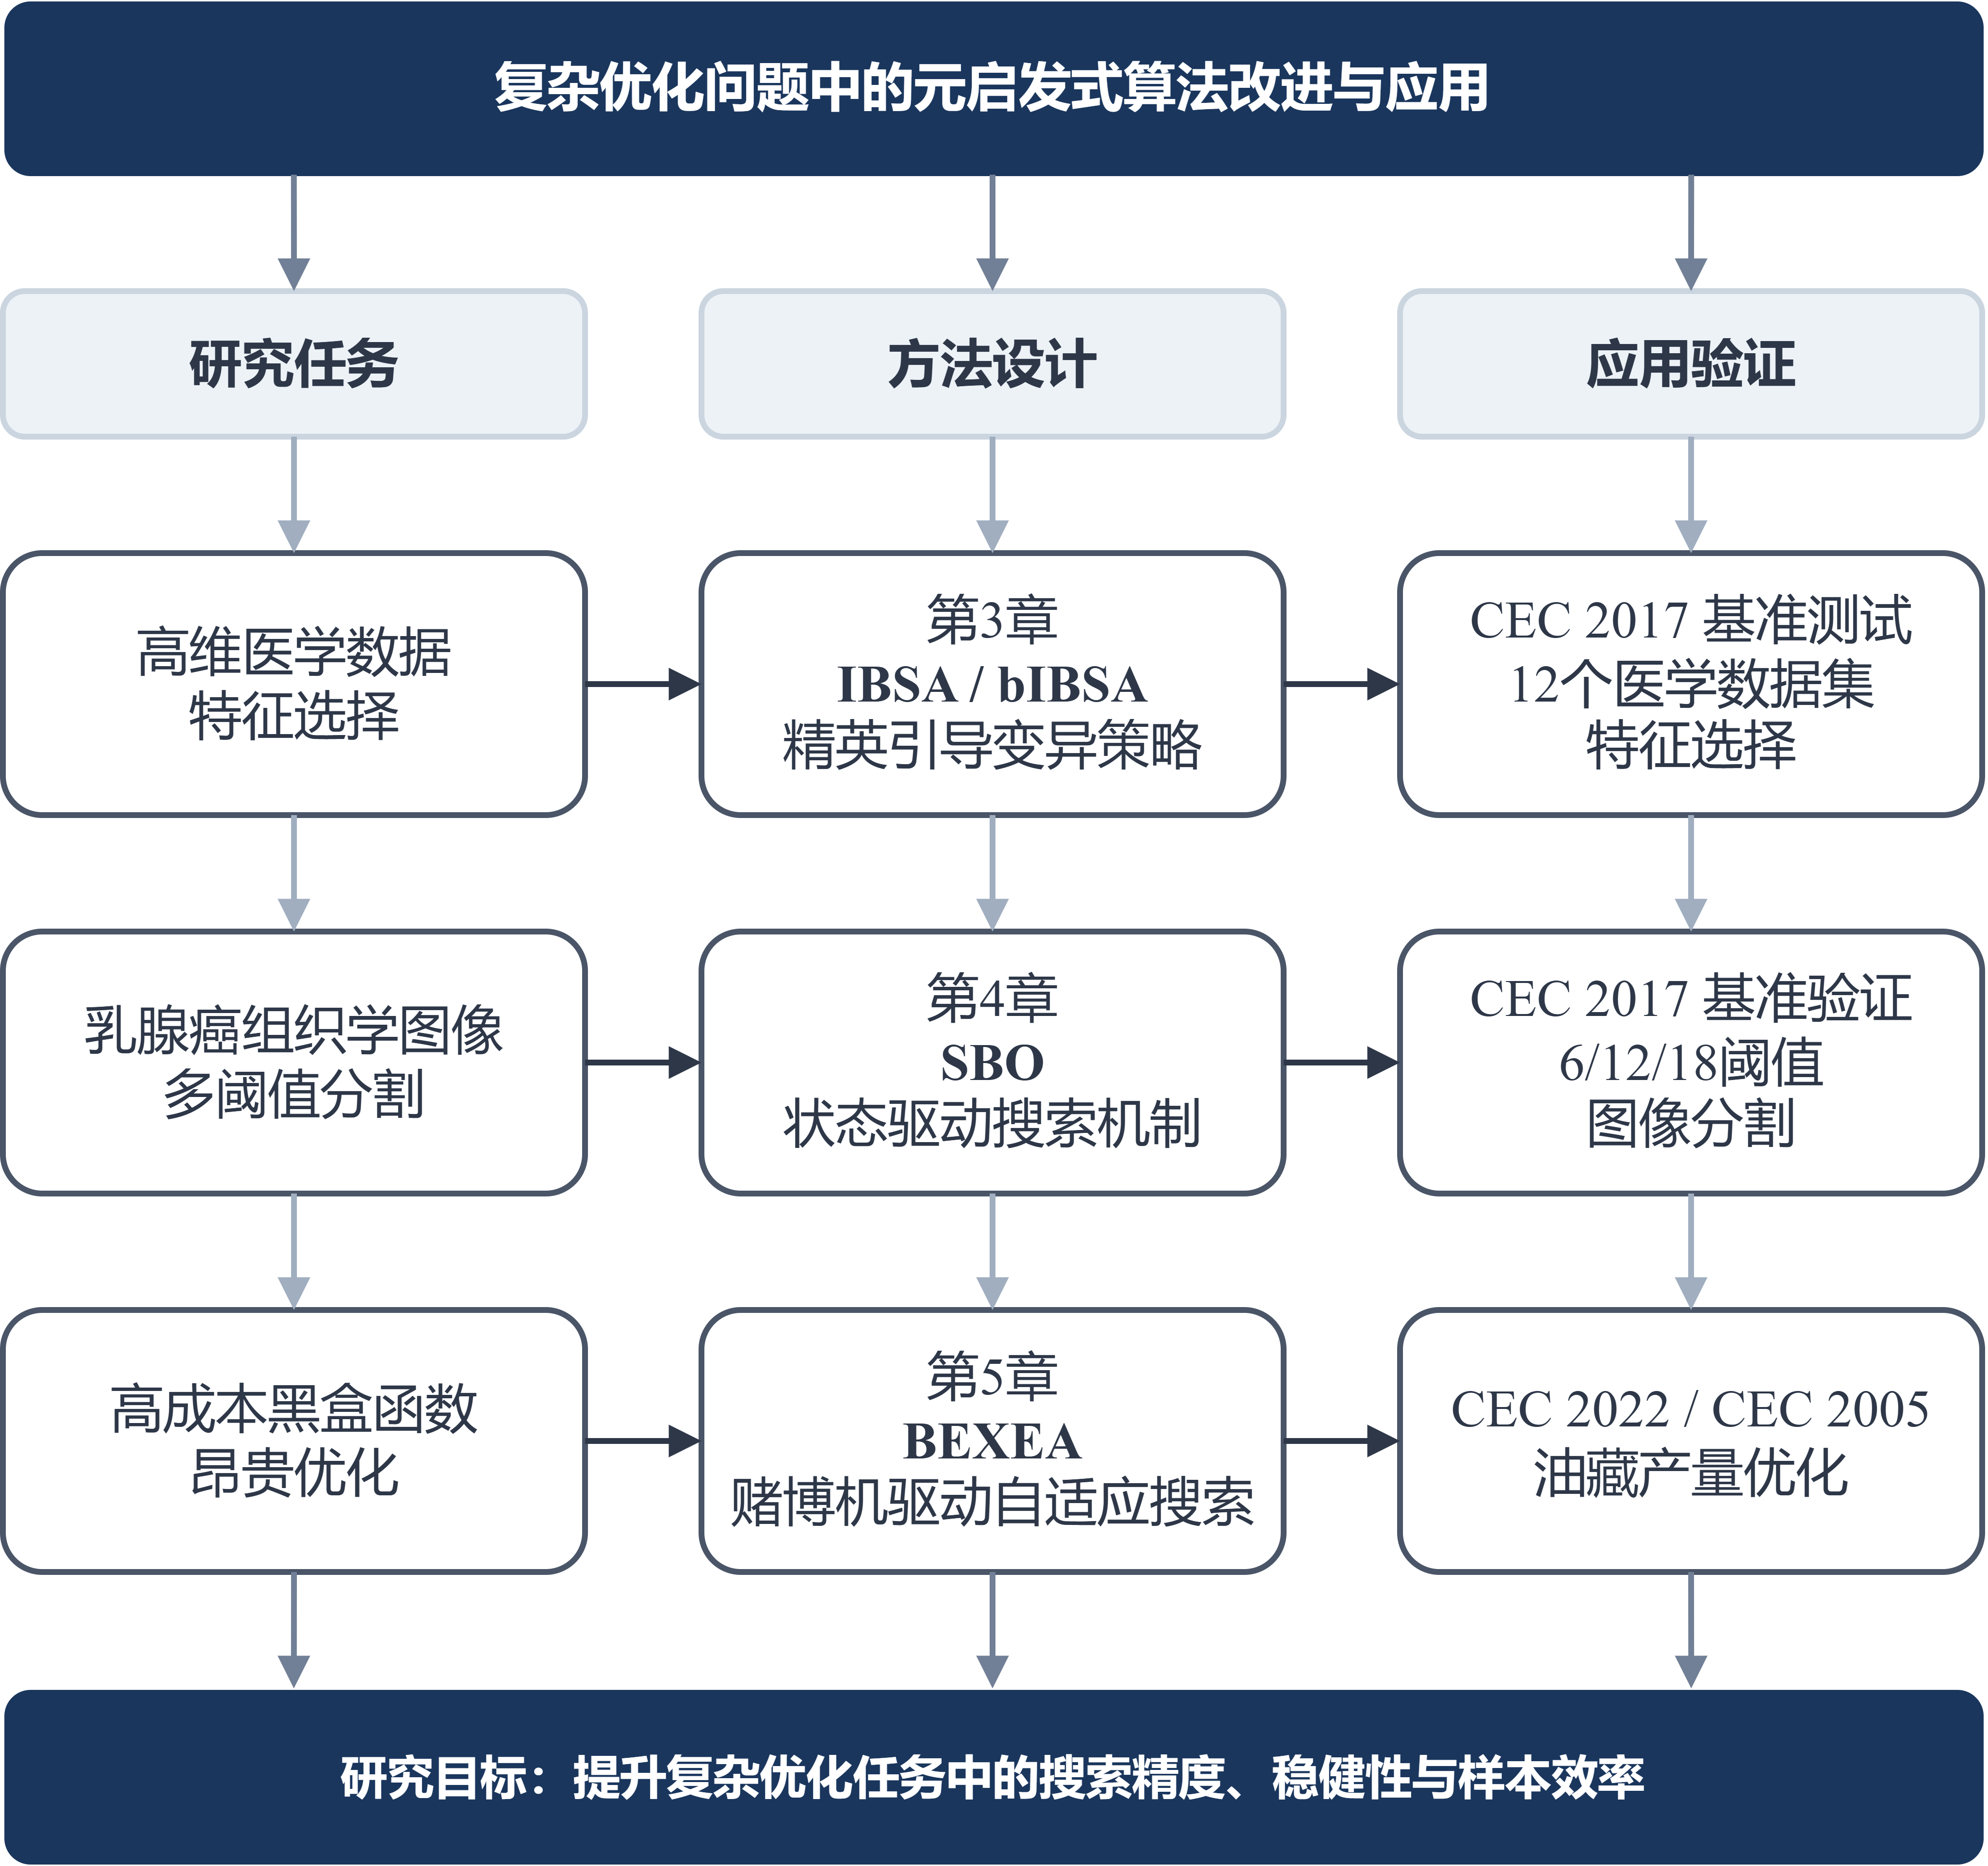
\includegraphics[width=0.96\textwidth]{figures/chapter1/thesis_overview_refined.drawio.png}
  \bicaption{总体技术框架图}{Framework diagram of the overall thesis}
  \label{fig:overall-framework}
\end{figure}

本研究以复杂任务中的共性瓶颈为导向，由三条平行的研究路径支撑：针对特征选择中的平衡性难题，提出IBSA及其离散变体bIBSA；针对图像分割中的策略协调问题，开发状态驱动的SBO算法；针对昂贵优化的效率挑战，构建赌博机驱动的BEXEA架构。各核心章节均遵循“算法建模—基准测评—工程验证”的叙事逻辑，确保论证过程的严密与统一。

从论证脉络看，各章节间并非简单的横向罗列，而是遵循了“既有框架优化、全新机制探索、复杂场景扩展”的演进逻辑。第三章聚焦BSA框架的精英信息挖掘，验证改进策略在多维场景下的适配度；第四章针对复杂连续域的控制难题，由浅入深地推导出全新的SBO算法，以增强状态感知能力；第五章则将视角延展至高成本优化领域，结合前序搜索机制，引入代理模型与赌博机决策，形成应对极低评估预算的BEXEA方案。

\section{本文组织结构安排}

本研究围绕特征选择、图像分割及昂贵优化三类典型任务，重点探讨元启发式算法的优化机理及其在工程中的应用实践。全文在阐明背景现状的基础上，分层次论述了三种改进算法的设计初衷、数学表征及应用效能。具体安排如下：

第一章，绪论：阐述课题背景与意义，评述国内外研究动态，并给出整体研究架构与章节脉络。

第二章，相关理论及技术：梳理后续研究的理论根基，包括元启发式搜索范式、应用场景数学建模、代理辅助技术、赌博机博弈理论及统计测评体系。

第三章，基于精英引导变异策略的改进回溯搜索算法：针对BSA在精英利用上的滞后问题，详细阐述IBSA的设计机理及其变异策略。通过基准函数测评与高维医学数据集筛选任务，验证其在精度与稀疏性上的优势。

第四章，基于状态的优化算法：针对复杂连续域寻优中的协调难题，推出全新的SBO算法，系统论证其状态驱动机制的科学性，并结合乳腺癌组织图像分割任务验证其实用价值。

第五章，基于赌博机驱动的自适应搜索代理辅助进化算法：面向评估预算高度受限的场景，论述BEXEA的自适应搜索策略与不确定性采样准则。通过标准昂贵优化测试集与实际油藏产量优化案例，评估其样本利用效率。

第六章，总结与展望：提炼主要创新点，剖析研究局限，并对智能优化领域的未来走向进行展望。
��


%%% Chapter 2: 相关理论及技术 (Related Theory and Technology)
% Chapter 2: 相关理论及技术 (Related Theory and Technology)
\chapter{相关理论及技术}

为了给后续各章的算法改进与应用验证提供坚实的理论支撑，本章将系统梳理研究所涉及的核心技术与理论框架。内容涵盖了元启发式搜索机制、复杂优化任务的数学建模、代理辅助优化策略，以及用于性能评估的统计分析方法。

\section{元启发式优化算法}

元启发式算法（MAs）已成为现代复杂优化领域的重要方法论基础，尤其在处理搜索空间庞大且缺乏显式解结构的NP-hard问题时，表现出显著的灵活性和鲁棒性\cite{ibsa_ref4,sbo_ref1}。这些方法按其灵感来源的多样性，通常被划分为群体智能、进化计算、自然规律模拟以及人类行为模仿等不同体系\cite{sbo_ref11}。尽管不同算法的更新机制各异，但其核心目标都在于协调探索（Exploration）与开发（Exploitation），即在扩大搜索范围和强化局部精炼之间取得平衡\cite{ibsa_ref75}。

\subsection{群体智能与进化算法}

群体智能算法通过个体间的信息共享与协同更新实现全局搜索\cite{sbo_ref18}。粒子群优化（PSO）\cite{ibsa_ref26}是其中最具代表性的方法之一，其基本更新规则为：
\begin{equation}
v_i^{t+1} = \omega v_i^t + c_1 r_1 (pbest_i - x_i^t) + c_2 r_2 (gbest - x_i^t)
\end{equation}
\begin{equation}
x_i^{t+1} = x_i^t + v_i^{t+1}
\end{equation}
其中，$\omega$为惯性权重，$c_1$和$c_2$为学习因子，$r_1$和$r_2$为$[0,1]$上的随机数，$pbest_i$和$gbest$分别表示个体历史最优位置与群体全局最优位置。PSO因概念简洁和实现高效，已被广泛应用于函数优化、神经网络训练和组合优化等领域。除PSO外，灰狼优化算法（GWO）\cite{ibsa_ref81}通过模拟灰狼的社会等级和狩猎行为实现群体搜索，蚁群优化算法（ACO）\cite{ibsa_ref25}借鉴蚂蚁信息素沉积机制解决离散优化问题，人工蜂群算法（ABC）\cite{ibsa_ref27}模拟蜜蜂觅食行为进行全局搜索。这些算法各有特色，共同构成了群体智能优化方法的基本框架。

与模拟群体行为不同，进化算法更侧重于遗传变异规律的工程模拟\cite{sbo_ref11}。差分进化（DE）\cite{ibsa_ref34}结构简洁，在实值优化任务中收敛稳定，已成为代理辅助优化中的常用搜索工具。常用的DE/rand/1变异策略通过向量间的差分驱动搜索：
\begin{equation}
v_i = x_{r1} + F \cdot (x_{r2} - x_{r3})
\end{equation}
其中，缩放因子$F$与交叉概率$CR$共同调控了变异幅度和个体多样性。这种贪心驱动的迭代机制不仅保证了收敛的稳定性\cite{ibsa_ref55}，也为后续各章的算法设计提供了基本的种群演化框架。

\subsection{回溯搜索算法}

回溯搜索算法（BSA）由Civicioglu\cite{ibsa_ref53}于2013年提出，是一种利用历史种群记忆进行搜索的进化算法。其主要流程包括初始化、Selection-I、变异、交叉和Selection-II五个阶段，其中变异策略利用当前种群与历史种群之间的差异生成候选解：
\begin{equation}
\boldsymbol{Mutant} = \boldsymbol{X} + F \cdot (\boldsymbol{OldX} - \boldsymbol{X})
\end{equation}
其中，$F = 3 \cdot rndn$。历史记忆策略提升了全局探索的潜力，但由于变异与交叉逻辑带有较强的随机性，在局部精细化搜索方面仍有不足\cite{ibsa_ref63}。Zhao\cite{ibsa_ref57}与Nama\cite{ibsa_ref59}等学者提出的策略改进方案，直接启发了本文在第三章中对IBSA算法的设计思路。

\subsection{探索与开发平衡性}
\label{sec:ch2_balance_diversity}

为定量分析算法在搜索过程中的动态行为，本研究引入基于种群多样性的度量指标。维度多样性$\text{Div}(t)$定义为：
\begin{equation}
\text{Div}(t)=\frac{1}{D}\sum^D_{j=1}{\frac{1}{N}\sum^N_{i=1}{\left|\operatorname{median}\left(X^j\left(t\right)\right)-X^j_i\left(t\right)\right|}}
\end{equation}

在此基础上，探索率与开发率分别定义为：
\begin{equation}
\text{Exploration}=\frac{\text{Div}\left(t\right)}{\text{Div}_{\max}}\times 100\%
\end{equation}
\begin{equation}
\text{Exploitation}=\frac{\left|\text{Div}\left(t\right)-\text{Div}_{\max}\right|}{\text{Div}_{\max}}\times 100\%
\end{equation}
进一步地，基于种群质心的欧氏距离多样性$I_C(t)$为：
\begin{equation}
I_C(t) = \sqrt{\sum^{N}_{i=1}{\sum^{D}_{j=1}{{\left(X^j_i\left(t\right)-C^j(t)\right)}^{2}}}}
\end{equation}
\begin{equation}
C^j(t) = \frac{1}{N}\sum^N_{i=1}{X^j_i\left(t\right)}
\end{equation}
$I_C(t)$越大，种群整体分散程度越高，说明算法处于探索阶段；$I_C(t)$较小时种群趋于聚集，算法处于开发阶段。较理想的优化过程应在搜索前期保持较高的多样性，并在后期逐步收缩以精炼最优解。第三章和第四章将利用这些指标分析所提算法的搜索特性。

\section{特征选择与图像分割问题简介}

本研究所涉及的两个主要应用场景——高维特征筛选与医学影像分割，本质上均是对候选参数的寻优过程。前者需要在离散组合空间中搜索最优特征子集，后者则是在连续或准离散的灰度阈值空间中寻找最优分割参数。

\subsection{特征选择问题定义}

特征选择（FS）旨在从原始特征中筛选出对任务贡献最大的子集，在保持或提升模型性能的同时降低维度，缓解维数灾难并增强可解释性\cite{ibsa_ref50}。常见方法包括过滤式、嵌入式和包裹式三类\cite{sbo_ref61}：过滤式依赖统计指标进行独立筛选，计算效率高但难以刻画特征交互\cite{sbo_ref62}；嵌入式将特征选择融入模型训练过程；包裹式直接以分类器性能评价特征子集，效果通常更好，但计算成本较高\cite{ibsa_ref23,sbo_ref64}。

在基于元启发式的包裹式特征选择中，每个特征对应一个0/1决策变量，问题可视为二值优化。由于多数元启发式算法面向连续空间，通常需借助V型传递函数完成二值化：
\begin{equation}
T(x) = \left| \operatorname{erf}\left(\frac{\sqrt{\pi}}{2} x\right) \right|
\end{equation}
若$T(x_i^d) > rand$，则对应维度取值翻转，否则保持不变。为同时兼顾分类误差和特征压缩率，适应度函数定义为：
\begin{equation}
\text{Fitness}=\alpha\cdot \gamma_R\left(N\right)+\beta\cdot \frac{\left|R\right|}{\left|N\right|}
\end{equation}
后续实验将从平均适应度、分类错误率、选择特征数和运行时间四个方面评估算法表现。

\subsection{多阈值图像分割问题}

多阈值图像分割通过确定多个阈值将图像灰度空间划分为若干区域，是医学图像分析中的常见预处理步骤\cite{sbo_ref79,sbo_ref80}。若图像灰度级为$L$，阈值向量可表示为：
\begin{equation}
\boldsymbol{T} = [t_1, t_2, \ldots, t_K], \quad 0 \le t_1 < t_2 < \cdots < t_K \le L-1
\end{equation}
其中$K$为阈值个数。随着$K$增加，候选解空间迅速膨胀，传统穷举方法难以在可接受时间内获得满意解。利用元启发式算法在这类大规模搜索空间中高效搜索最优阈值组合，已成为该领域的主流做法\cite{sbo_ref82}。本文第四章采用Renyi熵评价阈值集合质量，并利用元启发式算法搜索最优阈值，以提高乳腺癌组织学图像\cite{sbo_ref83}的分割效果。

\section{代理辅助昂贵优化技术}

在昂贵优化问题（EOPs）中，单次目标函数评估通常依赖高保真仿真或复杂工程计算，代价极高\cite{liu2023airfoils,kumar2024optimization}。代理辅助进化算法（SAEAs）通过低成本模型近似真实目标函数，以减少真实评估次数\cite{he2023review,jin2018data}，是第五章方法设计的理论基础。

\subsection{代理模型与填充准则}
\label{sec:ch2_surrogate_models}

代理模型用于学习真实目标函数的近似映射\cite{kudela2022recent}。径向基函数（RBF）模型是一种基于距离的插值方法\cite{regis2013evolutionary}，其预测值为已知样本点处基函数的加权组合：
\begin{equation}
\hat{f}(x) = \sum_{i=1}^{n} \lambda_i \phi(\|x - x_i\|)
\end{equation}
由插值条件$\hat{f}(x_i) = f(x_i)$可得矩阵形式：
\begin{equation}
\mathcal{F} = \boldsymbol{\Psi} \mathcal{W}
\end{equation}
其中$\boldsymbol{\Psi}_{ij} = \phi(\|x_i - x_j\|)$。RBF模型训练速度快、插值精度高，对高维问题适应性较好\cite{kudela2022recent}，因此在第五章中被选作基础代理模型。

图\ref{fig:ch2_RBF_prediction}展示了利用六个均匀分布样本对一维函数进行RBF近似的结果\cite{forrester2008engineering}。白色圆圈表示样本点，黑色实线代表真实适应度景观，红色虚线代表RBF预测函数。从图中可以看出，RBF模型在样本点处能够精确插值，而在样本点之间给出平滑近似。

\begin{figure}[!b]
    \centering
    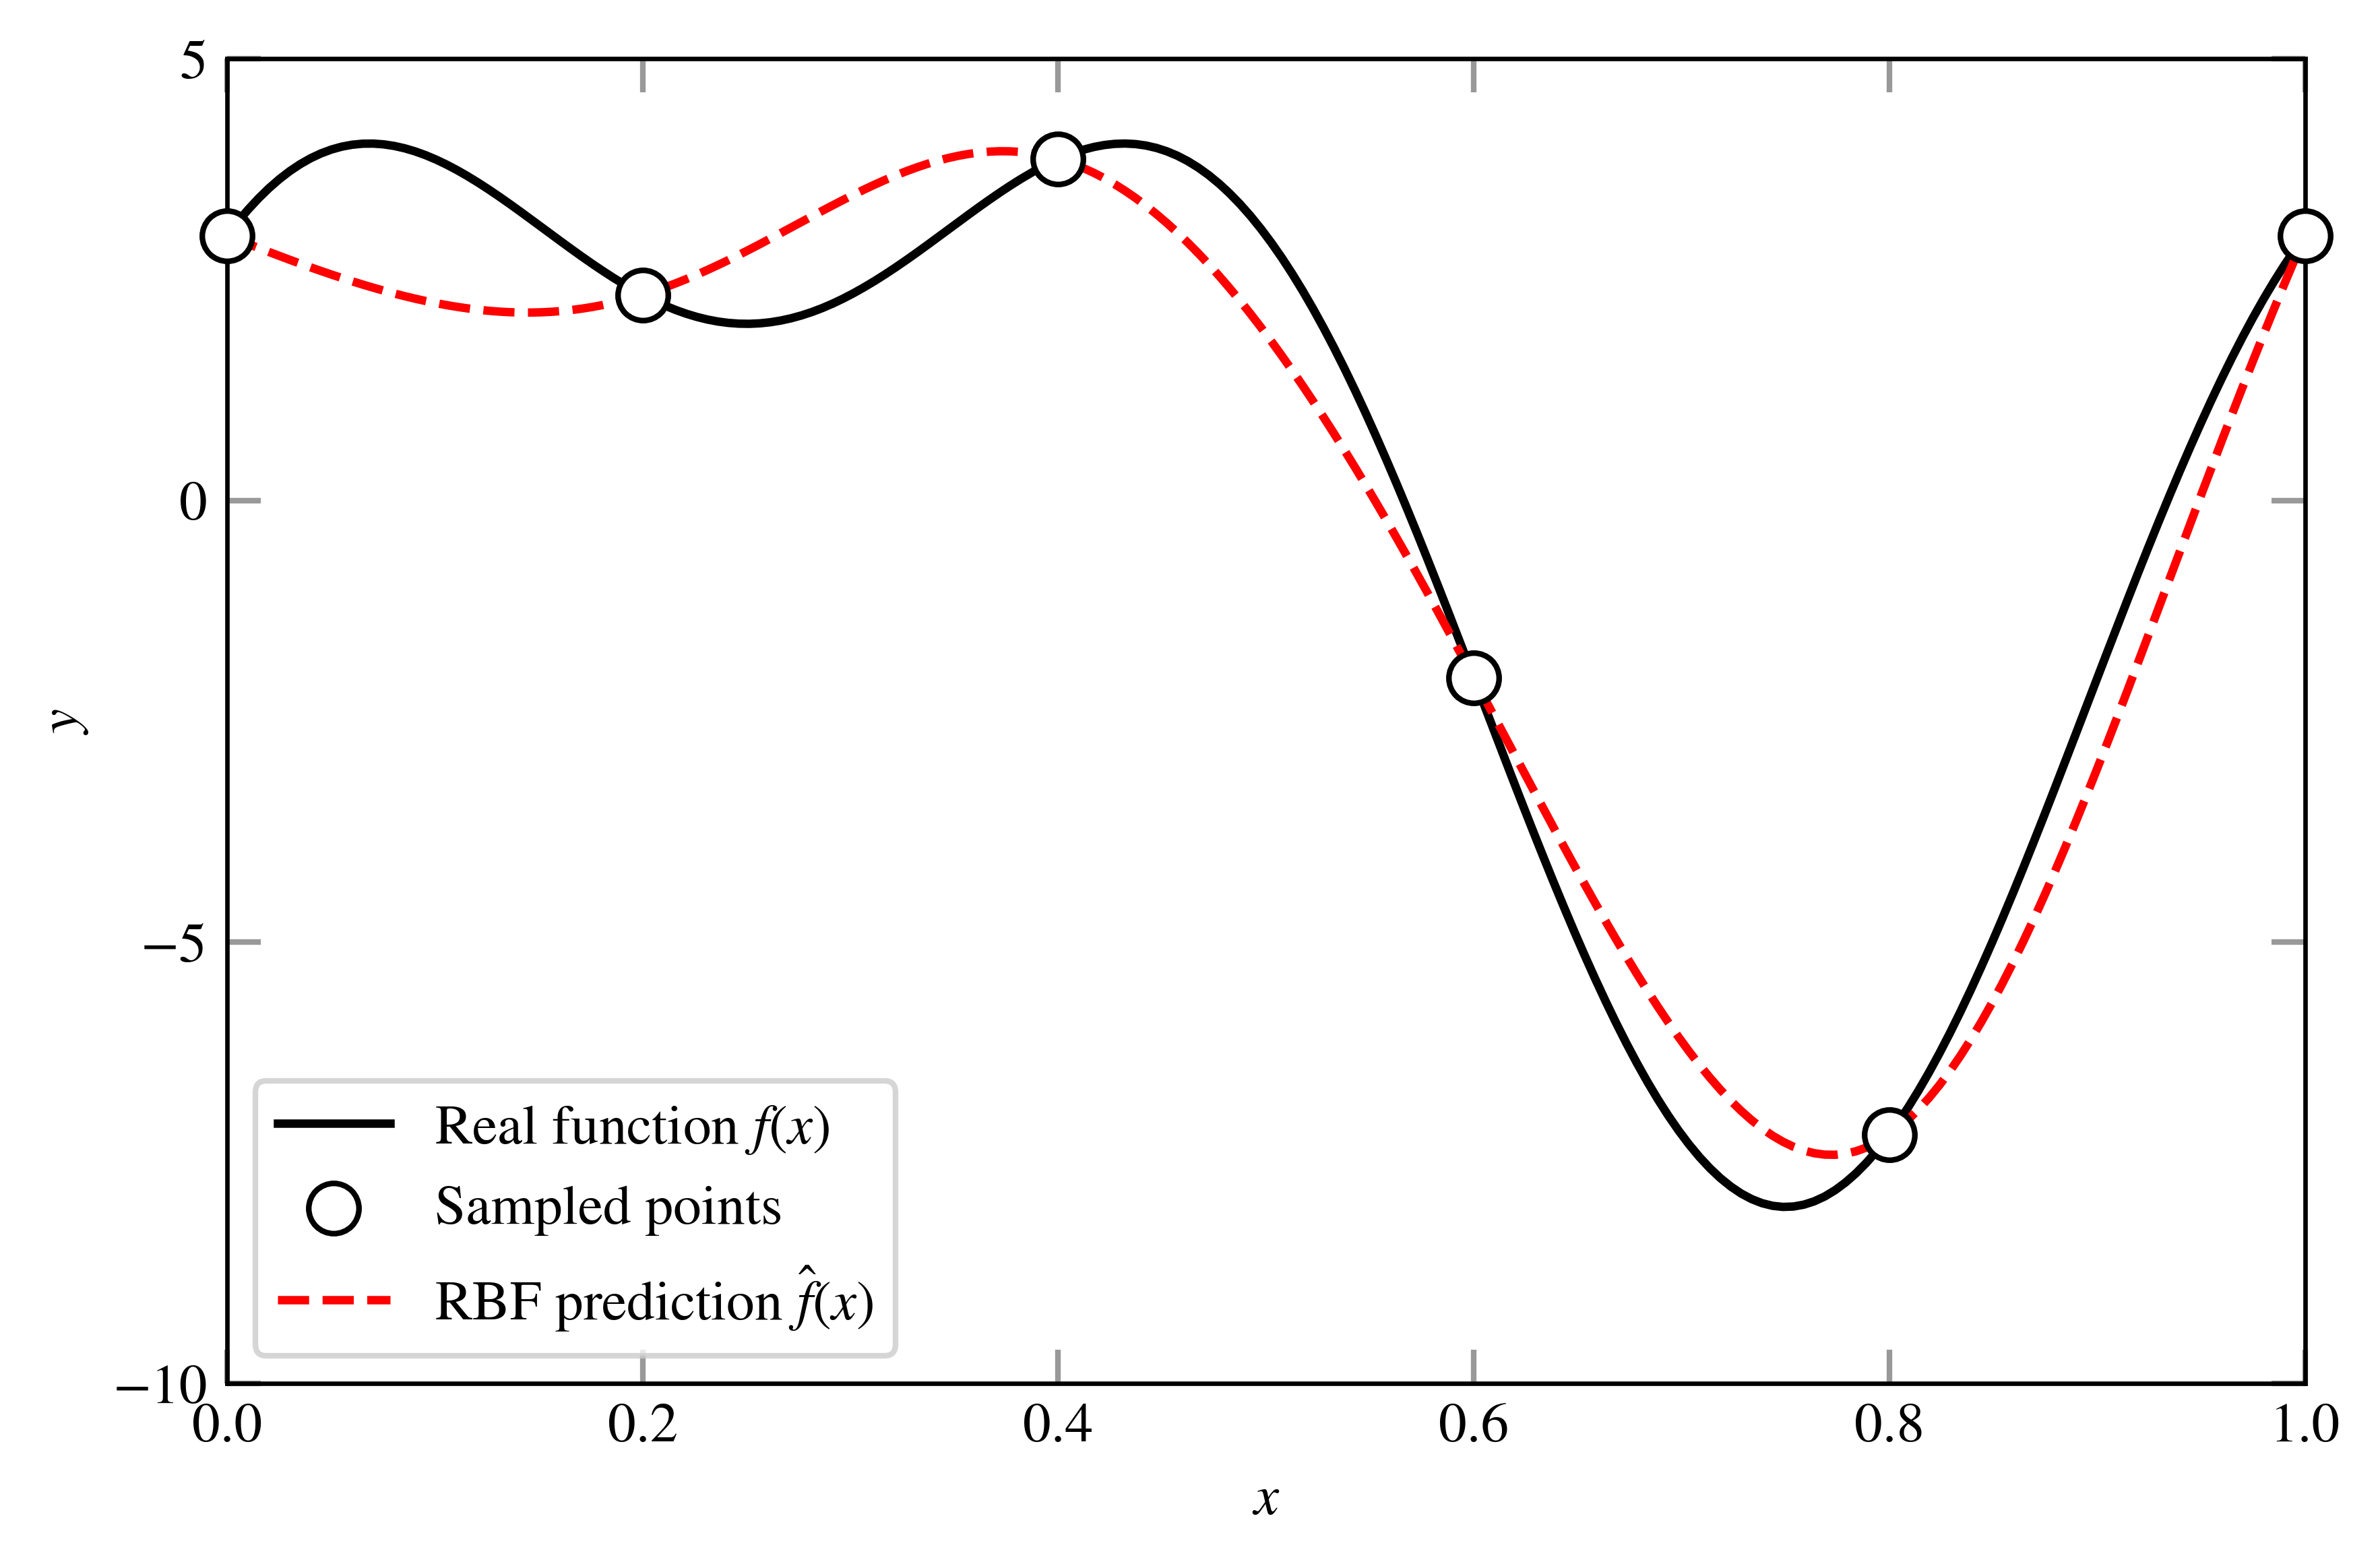
\includegraphics[width=0.92\linewidth]{figures/chapter5/rbf_plot.png}
    \bicaption{一维函数上的RBF预测}{RBF prediction on a 1-dimensional function}
    \label{fig:ch2_RBF_prediction}
\end{figure}

Kriging模型（高斯过程模型）\cite{buche2005accelerating,liu2013gaussian}除给出预测值外，还能提供不确定性估计，因此常与采样决策联合使用。为从候选解中筛选最值得进行真实评估的样本，通常需要引入填充准则\cite{zhan2020expected}。期望改进（EI）\cite{jones1998efficient}定义为：
\begin{equation}
EI(x) = (f_{min} - \hat{f}(x)) \Phi\left(\frac{f_{min} - \hat{f}(x)}{s(x)}\right) + s(x) \phi\left(\frac{f_{min} - \hat{f}(x)}{s(x)}\right)
\end{equation}
其中，$f_{min}$为当前最优值，$\hat{f}(x)$和$s(x)$分别为代理模型的预测均值和标准差，$\Phi$和$\phi$分别为标准正态分布的累积分布函数和概率密度函数。置信下界（LCB）则定义为：
\begin{equation}
LCB(x) = \hat{f}(x) - \kappa \cdot s(x)
\end{equation}
其中，$\kappa$越大则越倾向于探索。EI和LCB都体现了对探索与开发的联合考虑，使代理辅助优化能够在有限评估预算下做出较合理的采样决策。

\subsection{多臂赌博机策略}

多臂赌博机（MAB）问题描述了决策者如何在多个候选动作之间权衡已知高收益选择与未知选择\cite{slivkins2019introduction}，其核心是探索与开发的平衡。在优化算法中，可将不同搜索算子视为不同臂，根据环境反馈自适应地调整选择概率\cite{xie2023surrogate,gong2024surrogate}。

上置信界（UCB）策略是解决MAB问题的经典方法之一\cite{auer2002finite}，其在第$t$轮选择具有最高上置信界的臂：
\begin{equation}
a_t = \argmax_{a} \left[ Q_t(a) + c \sqrt{\frac{\ln t}{N_t(a)}} \right]
\end{equation}
其中，$Q_t(a)$为臂$a$的估计收益均值，$N_t(a)$为臂$a$被选择的次数，$c$为探索系数。UCB策略的核心在于：$Q_t(a)$鼓励选择历史表现较好的臂（利用），探索项$c \sqrt{\ln t / N_t(a)}$则鼓励尝试被选次数较少的臂（探索），随着总选择次数增长，探索项逐步衰减，策略自然收敛到最优臂。第五章将在此基础上引入赌博机驱动的自适应搜索机制，将不同搜索模式建模为不同臂，根据实时优化反馈动态切换搜索策略。

\section{基准测试与统计检验}

\subsection{基准测试函数}

基准测试函数为算法性能评估提供了统一且可复现的比较环境\cite{ibsa_ref4}。IEEE CEC 2017测试套件包含30个函数，覆盖单峰（F1--F3）、多峰（F4--F10）、混合（F11--F20）和组合（F21--F30）四类问题\cite{ibsa_ref88}，能够全面考察算法在不同搜索景观下的表现，本文第三章和第四章均采用该测试套件。IEEE CEC 2022测试套件面向函数评估受限的昂贵优化场景，包含12个函数\cite{kumar2024optimization}，最大评估次数受到严格限制，本文第五章使用其评估BEXEA的性能。

\subsection{统计检验方法}
\label{sec:ch2_stat_tests}

为保证实验比较的统计有效性，本文采用非参数统计检验对算法结果进行严格分析。Wilcoxon秩和检验\cite{ibsa_ref95}是一种成对比较方法，通过对两组独立样本的排名差异进行分析，判断二者是否具有统计显著性差异，适合样本量较小或数据不满足正态分布假设的情况。Friedman检验\cite{derrac2011practical}则是一种多组比较方法，可同时对多个算法在多个测试函数上的排名进行整体比较，排名越低表示综合表现越好。后续各章中，符号"+"、"="和"-"分别表示所提算法在Wilcoxon检验中显著更优、结果相当和显著更差，显著性水平设为$\alpha=0.05$。

\section{本章小结}

本章围绕后续研究的共性需求，对元启发式优化算法、特征选择与图像分割问题、代理辅助昂贵优化技术以及基准测试与统计检验方法进行了概述。这些内容为第三章至第五章的算法设计、应用建模和实验分析提供了统一的理论基础。






%%% Chapter 3: IBSA - Elite Leading Mutation Backtracking Search Algorithm
% Chapter 3: IBSA - Elite Leading Mutation Backtracking Search Algorithm

\chapter{基于精英引导变异策略的改进回溯搜索算法}
\label{chap:ibsa}

\section{引言}

在机器学习、大规模数据挖掘及生物信息工程等领域，全局优化与特征选择始终是核心研究课题\cite{ibsa_ref7,ibsa_ref13,ibsa_ref15}。然而，随着问题维度的提高，搜索空间的爆炸式增长使得这些问题具有极高的计算复杂度\cite{ibsa_ref1,ibsa_ref3,ibsa_ref5}。传统确定性算法在处理高维非凸搜索空间时，往往难以在合理时间内找到高质量解。因此，研究更具鲁棒性和普适性的近似优化策略具有重要的现实意义。

特征选择属于典型的组合优化范畴，通过从原始特征空间中剔除冗余信息并筛选判别力强的特征子集，能够有效增强分类模型的泛化性能\cite{ibsa_ref17,ibsa_ref18}。与过滤式方法相比，包裹式方法通过将搜索策略与分类算法结合，能更有效地捕捉特征间的非线性关联\cite{ibsa_ref20,ibsa_ref22,ibsa_ref23}。但随之而来的挑战是，庞大的候选子集空间显著增加了寻优的难度。

针对这些复杂寻优难题，元启发式算法凭借其不依赖梯度信息且实现灵活的优势，在诸多求解场景中展现出良好效果\cite{ibsa_ref24}。进化算法、群智能优化等路线在各自擅长的场景中均有不俗表现\cite{ibsa_ref25,ibsa_ref29,ibsa_ref33,ibsa_ref37}。但一旦面对高维特征选择任务，现有方法普遍暴露出局部开发不足、参数调整繁琐以及收敛速度受限等问题\cite{ibsa_ref41,ibsa_ref50,ibsa_ref51}。

为克服现有方法的局限性，本章构建了涵盖连续空间优化与离散特征选择的完整验证框架。首先在标准测试函数上检验算法的搜索效率与精度，随后将其应用于医学高维特征选择任务，以期全面评估算法的改进效果与实际应用价值。

回溯搜索算法（BSA）因结构精炼、参数负载轻而在工程领域备受关注\cite{ibsa_ref53}。但其原有的变异与交叉机制过于偏重全局探索，对种群中优秀个体的利用不足，限制了其在高精度优化问题上的表现。为此，本章提出了一种集成精英引导变异策略的改进回溯搜索算法（IBSA），并衍生出适用于特征选择的二值化版本（bIBSA）。IBSA通过加强精英解的引导作用，并结合V型传递函数实现离散空间的映射，优化了搜索过程的动态平衡。通过与23种算法在CEC 2017基准集上的对比，以及在特征选择任务中与8种主流算法的竞争，验证了新算法的有效性。主要贡献如下：

\begin{enumerate}
\item 针对BSA精英信息利用不足的问题，提出精英引导变异策略：对精英个体采用以当前最优解为基点的定向变异，对非精英个体引入自适应扰动向量$m$，随迭代进程动态收缩扰动幅度，区别化地增强种群的局部开发能力。

\item 引入停滞感知参数$s$，通过非线性映射得到切换概率$p$，自适应地在全局交叉与局部交叉之间动态切换，并联动更新历史种群$OldX$，改善BSA原有的随机交叉选择机制，提升探索与开发的平衡性。

\item 构造二值版本bIBSA，结合V型传递函数与KNN分类器，将IBSA扩展至高维包裹式特征选择任务。

\item 在CEC 2017基准函数（连续优化）和21个UCI数据集（特征选择）上开展系统实验，与23种及8种对比算法进行全面比较，验证IBSA和bIBSA的有效性与鲁棒性。
\end{enumerate}

本章后续内容组织如下：第2节详述IBSA的改进机理、二值化扩展方案及其计算成本分析；第3节通过对比实验评估算法性能；第4节总结全章研究。


\section{IBSA算法及其特征选择方法}

本节将从设计思路、核心搜索算子的演变、二值特征筛选机制以及计算复杂度四个方面展开论述。


\subsection{研究动机}

参数配置往往决定了元启发式算法在全局探索与局部开发之间的平衡效能。通常情况下，这些参数需要大量的经验调试，不仅过程耗时\cite{ibsa_ref65}，且在处理不同问题时往往缺乏通用性。例如，模拟退火（SA）的效果高度依赖于温度参数的设置；差分进化算法（DE）对交叉率和变异率也非常敏感。即便是一些结构较简单的算法，如布谷鸟搜索算法（CSA）\cite{ibsa_ref66}，在处理特定场景时也需要精细调优，这增加了算法的落地成本。

为解决这一问题，研究者们尝试了多种自适应调参方法。然而，许多改进方案在更换应用场景时仍需重新调优，表现出较差的迁移能力。参数敏感性已成为限制SA、DE等经典算法以及现代群智能算法大规模工业应用的主要瓶颈。

回溯搜索算法（BSA）采用独特的双种群协作机制，通过维护历史种群并在搜索过程中引入回溯信息，能有效拓宽搜索边界，防止陷入局部极值。算法的运行由初始化、历史信息选择（选择I）、变异映射、杂交（交叉）以及生存竞争（选择II）五个环节构成。各阶段的数学描述如下。

\textbf{（1）初始化：}初始种群按公式\eqref{ibsa_eq_1}在搜索空间内均匀随机生成。
\begin{equation}
\label{ibsa_eq_1}
X_i,_j=U(low_j,\ up_j)
\end{equation}
\noindent 其中，$i\in[1,N]$为个体索引，$j\in[1,D]$为维度索引，$low$和$up$分别为变量的下界和上界。

\textbf{（2）选择I：}该阶段维护历史种群$OldX$，为变异提供方向参考。$OldX$初始化方式与$X$相同（公式\eqref{ibsa_eq_2}），随后按公式\eqref{ibsa_eq_3}以一定概率更新为当前种群，并经公式\eqref{ibsa_eq_4}随机置换以增加多样性。
\begin{equation}
\label{ibsa_eq_2}
OldX_i,_j=U(low_j,\ up_j)
\end{equation}
\begin{equation}
\label{ibsa_eq_3}
OldX=
\begin{cases}
X, & a<b\\
OldX, & \text{otherwise}
\end{cases}
\end{equation}
\noindent 其中，$a$和$b$为$[0,1]$上的随机数。
\begin{equation}
\label{ibsa_eq_4}
OldX=permuting\left(OldX\right)
\end{equation}
$permuting(\cdot)$对$OldX$中的个体顺序进行随机打乱。

\textbf{（3）变异：}变异阶段利用$OldX$与当前种群$X$的差分信息生成变异种群$Mutant$，如公式\eqref{ibsa_eq_5}所示。
\begin{equation}
\label{ibsa_eq_5}
Mutant=X+F\mathrm{\times }\left(oldX-X\right)
\end{equation}
其中，幅度控制因子$F=3\times rndn$，$rndn$服从标准正态分布。

\textbf{（4）交叉：}交叉阶段通过二值映射矩阵$map$控制试验种群$T$的生成。$map$按概率选择全局交叉（公式\eqref{ibsa_eq_6}）或局部交叉（公式\eqref{ibsa_eq_7}），最终由公式\eqref{ibsa_eq_8}从$Mutant$和$X$中组合生成$T$。
\begin{equation}
\label{ibsa_eq_6}
map_i,_{u\left(1:\left\lceil M\mathrm{\times }rand\mathrm{\times }D\right\rceil \right)}=1\mathrm{\mid }u=permuting\left(1,2,3,\dots ,\ D\right),\ rand\in \left(0,\ 1\right)
\end{equation}
\begin{equation}
\label{ibsa_eq_7}
map_i,_{randi\left(D\right)}=1
\end{equation}
\begin{equation}
\label{ibsa_eq_8}
T_{i,j}=
\begin{cases}
Mutant_{i,j}, & map_{i,j}=1\\
X_{i,j}, & map_{i,j}=0
\end{cases}
\end{equation}
符号$\mathrm{\textrm{┌}}\mathrm{\ }\mathrm{\textrm{┐}}$为上取整函数，$M$为混合率，$permuting(\cdot)$对决策变量顺序随机打乱。

\textbf{（5）选择II：}采用贪婪准则逐一比较当前个体与试验个体的适应度，保留更优者进入下一代，如公式\eqref{ibsa_eq_9}所示。
\begin{equation}
\label{ibsa_eq_9}
X_i=
\begin{cases}
T_i, & f\left(T_i\right)<f\left(X_i\right)\\
X_i, & \text{otherwise}
\end{cases}
\end{equation}
其中，$f(\cdot)$为目标函数。

BSA凭借精简的参数设计展现出向无参数化方向演化的潜力。但在应对高维复杂场景时，其短板也逐渐显现：交叉模式的随机切换难以契合种群进化的动态特征\cite{ibsa_ref63}；且对精英个体的利用不足削弱了算法在高质量区域的挖掘深度\cite{ibsa_ref67}；此外，历史种群的盲目更新也导致搜索缺乏明确的方向。为此，本章提出精英引导变异策略，通过优化历史信息的利用方式并改进交叉机制，在保持全局探索能力的同时，提升了算法的局部开发精度。


\subsection{精英引导变异策略}

尽管BSA引入了回溯机制，但其对进化过程中产生的优良个体挖掘程度仍显不足\cite{ibsa_ref53}。这种精英信息的缺失，加之交叉概率生成的随机性，使得算法在面对大规模搜索空间时难以快速锁定最优区域，限制了最终的收敛精度。

为了实时捕捉种群的进化状态，本文设计了一个停滞感知参数$s$。该参数通过监控最优解的更新频率来调整搜索步调：当进化停滞时，$s$线性增长以增强探索动力；一旦发现更优解，$s$通过平方根衰减迅速回落。通过式\eqref{ibsa_eq_11}的非线性映射，将$s$转化为切换概率$p$，从而引导算法在全局探索与局部精炼之间灵活切换。
\begin{equation}
\label{ibsa_eq_10}
s=
\begin{cases}
\sqrt{s}, & \text{elite updated}\\
s+1, & \text{otherwise}
\end{cases}
\end{equation}
\begin{equation}
\label{ibsa_eq_11}
p\ =\frac{sqrt\left(\frac{t}{Max\_FEs}\right)}{1\ +\ exp\left(-s\right)}
\end{equation}
为了增强历史种群的导向性，改进后的$OldX$更新逻辑与当前的搜索模式挂钩。在全局交叉活跃的阶段，当代种群通常包含更丰富的空间信息，此时将其更新至历史库能为变异方向提供更有价值的参考。这种机制改变了BSA盲目的回溯方式，使历史信息的积累与搜索动态保持同步。
\begin{equation}
\label{ibsa_eq_12}
OldX=\ X\ \ \ if\ flag==1
\end{equation}
\begin{equation}
\label{ibsa_eq_13}
flag=
\begin{cases}
1, & \text{global crossover}\\
0, & \text{otherwise}
\end{cases}
\end{equation}
针对普通种群成员，本文引入了自适应扰动向量$m$。其扰动幅度随迭代进程从全空间逐步收缩。这种动态设计使算法在初期具备较强的随机游走能力以探索未知区域，后期则聚焦于局部搜索，在不损失多样性的前提下提升了寻优的精细度。
\begin{equation}
\label{ibsa_eq_14}
m_i=
\begin{cases}
1, & rand>\left(\frac{t}{Max\_FEs}\right)\wedge 3\\
unifrnd\left(-\frac{t}{Max\_FEs},\frac{t}{Max\_FEs}\right), & \text{otherwise}
\end{cases}
\end{equation}
通过对精英与非精英个体实施差异化控制，IBSA能促使最优个体在当前区域进行深度挖掘。虽然这增加了算法逻辑的复杂度，但由此带来的精英信息挖掘能力对于解决高维优化问题至关重要。变异算子与精英更新逻辑的调整如式\eqref{ibsa_eq_15}与式\eqref{ibsa_eq_16}所示。
\begin{equation}
\label{ibsa_eq_15}
{\mathrm{Mutant}}_{\mathrm{i}}=m_i*\left(X_i+F*map_i\ .*\left(OldX_i-X_i\right)\right)\ \ \ if\ i\sim =BestX\_idx
\end{equation}
\begin{equation}
\label{ibsa_eq_16}
{\mathrm{Mutant}}_{\mathrm{i}}=BestX+F*\left(OldX_i-X_i\right)\ \ \ if\ i==BestX\_idx
\end{equation}
\noindent 其中，下标$i$表示元素的索引，$F$为随机生成的控制因子。

最后，精英引导策略的核心逻辑由公式\eqref{ibsa_eq_10}--\eqref{ibsa_eq_16}及后续流程图呈现。


\subsection{IBSA算法}

IBSA在原有BSA架构中嵌入精英引导变异策略，着力改善了历史种群更新的盲目性及交叉模式选择的随机性。

BSA的双种群结构通过引入历史坐标系校准搜索方向，这种逻辑使其区别于PSO或DE等依赖当代反馈的算法。然而，由于$OldX$原有的更新准则缺乏对搜索态势的感知，导致全局探索与局部开发之间的衔接仍具有较大的偶然性，难以根据实际进化进程做出响应。

为此，IBSA从两个维度优化了搜索流程：首先，建立了与搜索模式联动的历史种群更新准则，在探索活跃期保留高质量样本，增强了回溯机制的“导航”作用；其次，通过改进的反馈链路实现搜索力度的自动聚焦——在陷入瓶颈时调动全局搜索，在收敛迹象明显时则强化局部开发。

IBSA的主要步骤如下：

\textbf{步骤1~~初始化：}准备变量$X$、$OldX$、$BestFitness$、$PreBestFitness$、$BestX$、$map$、$s$和$flag$。

\textbf{步骤2~~选择-I：}通过比较适应度的变化计算$s$，并根据$flag$决定是否更新历史种群。

\textbf{步骤3~~变异和交叉：}根据$s$确定切换概率$p$，选择相应的变异策略，并更新$flag$。

\textbf{步骤4~~选择-II：}根据适应度优劣迭代更新$X$，同步更新当前最优解$BestX$。

上述过程循环执行直到满足终止条件。IBSA算法流程如图\ref{fig:flowchart_IBSA}所示。


\begin{figure}[htbp]
  \centering
  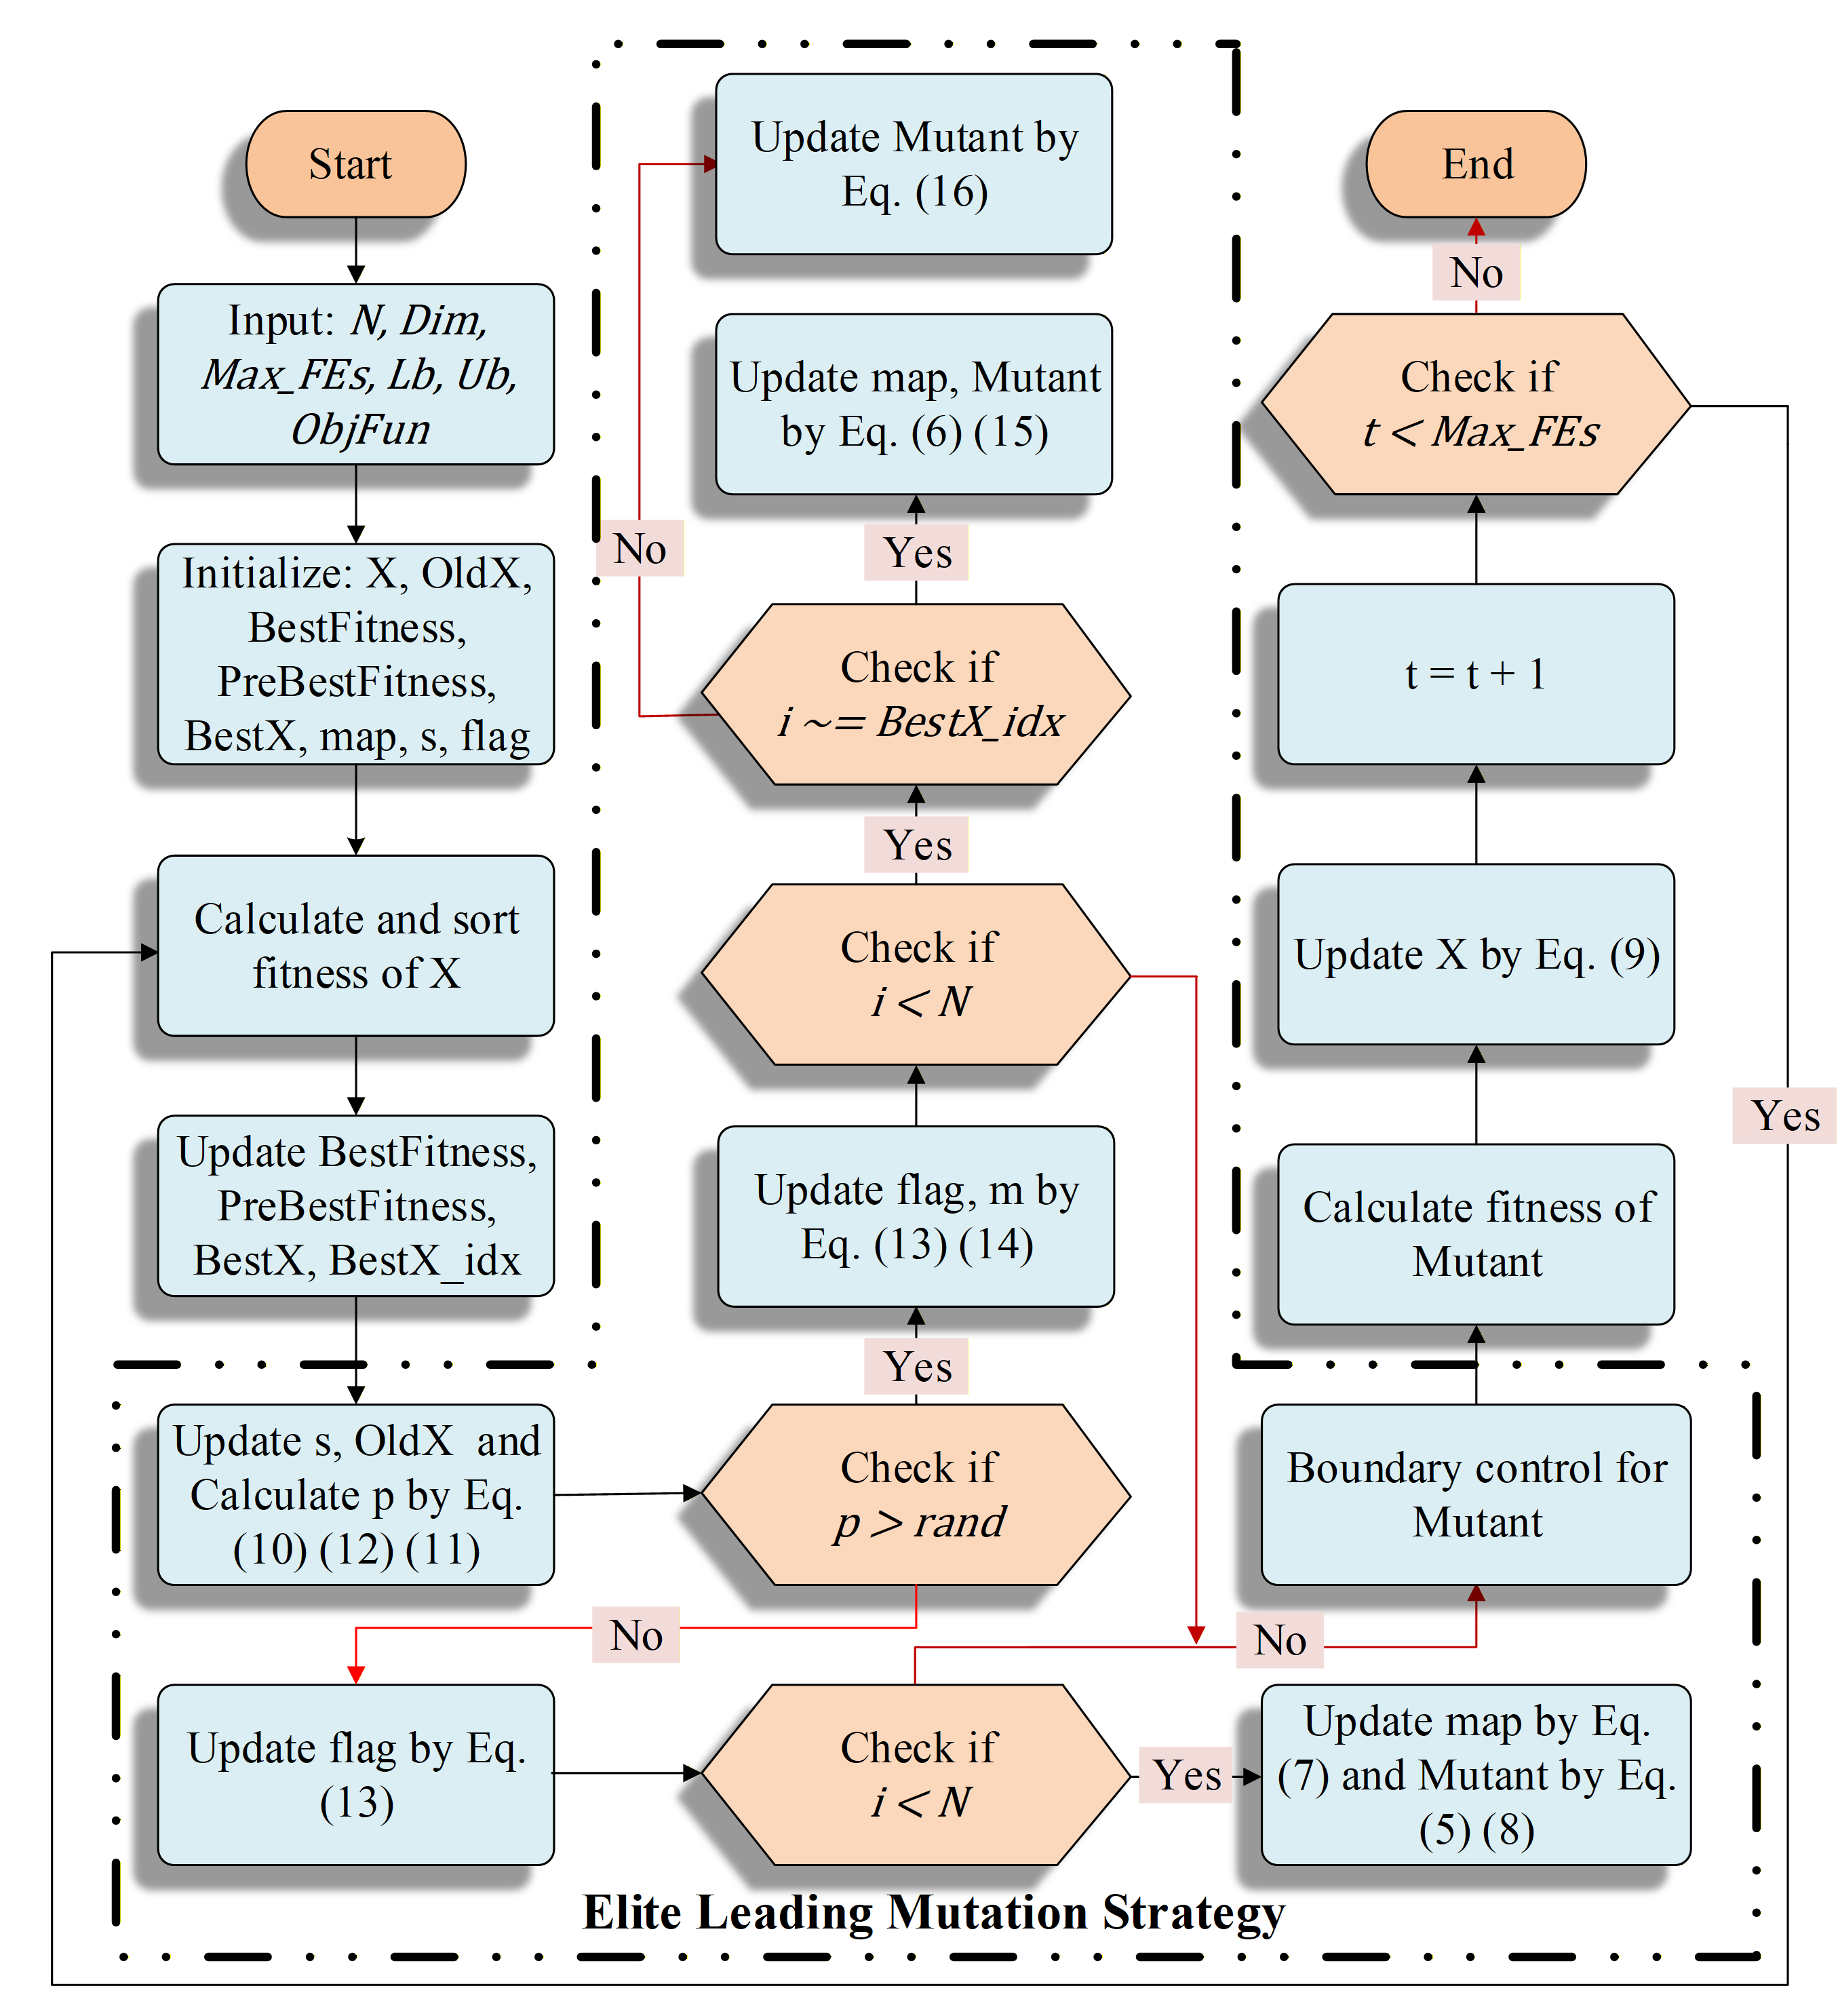
\includegraphics[width=\textwidth]{figures/chapter3/fig2_flowchart_IBSA.png}
  \bicaption{IBSA算法流程图}{Flowchart of IBSA}
  \label{fig:flowchart_IBSA}
\end{figure}


\subsection{bIBSA特征选择方法}

为处理离散空间问题，本章进一步衍生出二值化版本bIBSA，并将其应用于特征选择任务。面对给定$n$个特征产生的$2^n$种组合，bIBSA致力于高效搜寻最优子集。

为了在庞大的组合空间中有效寻优，bIBSA采用了与KNN分类器\cite{ibsa_ref70}结合的包裹式评估框架。在该框架下，每一组特征候选集都通过实际分类性能来判定优劣。虽然这种方式因频繁调用分类器而增加了计算成本，但它能直接反映特征间的非线性关联，在医学诊断等高精度场景中具有不可替代的价值。图\ref{fig:wrapper_feature_selection}展示了该评估流程。

为了使IBSA能够处理离散问题，本研究引入了V型传递函数\cite{ibsa_ref71}。在离散的超立方体搜索空间内，决策变量的演化被抽象为在顶点间的跃迁。传递函数将连续的搜索步长转换为比特翻转的概率，使bIBSA既能继承原算法良好的动态平衡特性，又能在高维特征选择任务中保持寻优的灵敏性。

V型函数将连续位置映射为翻转概率。若该概率表明翻转可能改善适应度，则执行翻转（公式\eqref{ibsa_eq_18}）；否则保持原值。这一机制使搜索代理能够在二值空间的顶点间有效探索。
\begin{equation}
\label{ibsa_eq_17}
V\left(X^j_i\left(t\right)\right)=\left|\frac{2}{\pi}*\mathrm{atan}\mathrm{}\left(\frac{\pi}{2}*X^j_i\left(t\right)\right)\right|
\end{equation}
\begin{equation}
\label{ibsa_eq_18}
X^j_i\left(t+1\right)=
\begin{cases}
1, & r\ge V\left(P^j_i\left(t\right)\right)\\
0, & r<V\left(P^j_i\left(t\right)\right)
\end{cases}
\end{equation}
\noindent 其中，$X^j_i\left(t\right)$表示第$t$次迭代中第$i$个代理在第$j$维的位置。

特征优化的过程本质上是特征数量与分类精度之间的博弈。在剔除冗余特征以降低维度的同时，必须保证模型的分类性能。这种对“简洁”与“高效”之间平衡的追求，驱动着bIBSA不断修正其搜索路径。

每个潜在解都通过公式\eqref{ibsa_eq_19}所示的适应度函数进行评估，该函数综合考虑了错误率和特征子集的大小。
\begin{equation}
\label{ibsa_eq_19}
Fitness=\alpha\cdot \gamma_R\left(N\right)+\beta\cdot \frac{\left|R\right|}{\left|N\right|}
\end{equation}
\noindent 其中，$\gamma_R(\cdot )$表示错误率函数，$R$和$N$分别为所选特征数和总特征数。为了平衡两个目标，本文将权重系数$\alpha$设定为0.05，$\beta$设定为0.95 \cite{ibsa_ref72}。这一比例引导算法在保证精度的前提下寻找尽可能小的特征集合。

\begin{figure}[htbp]
  \centering
  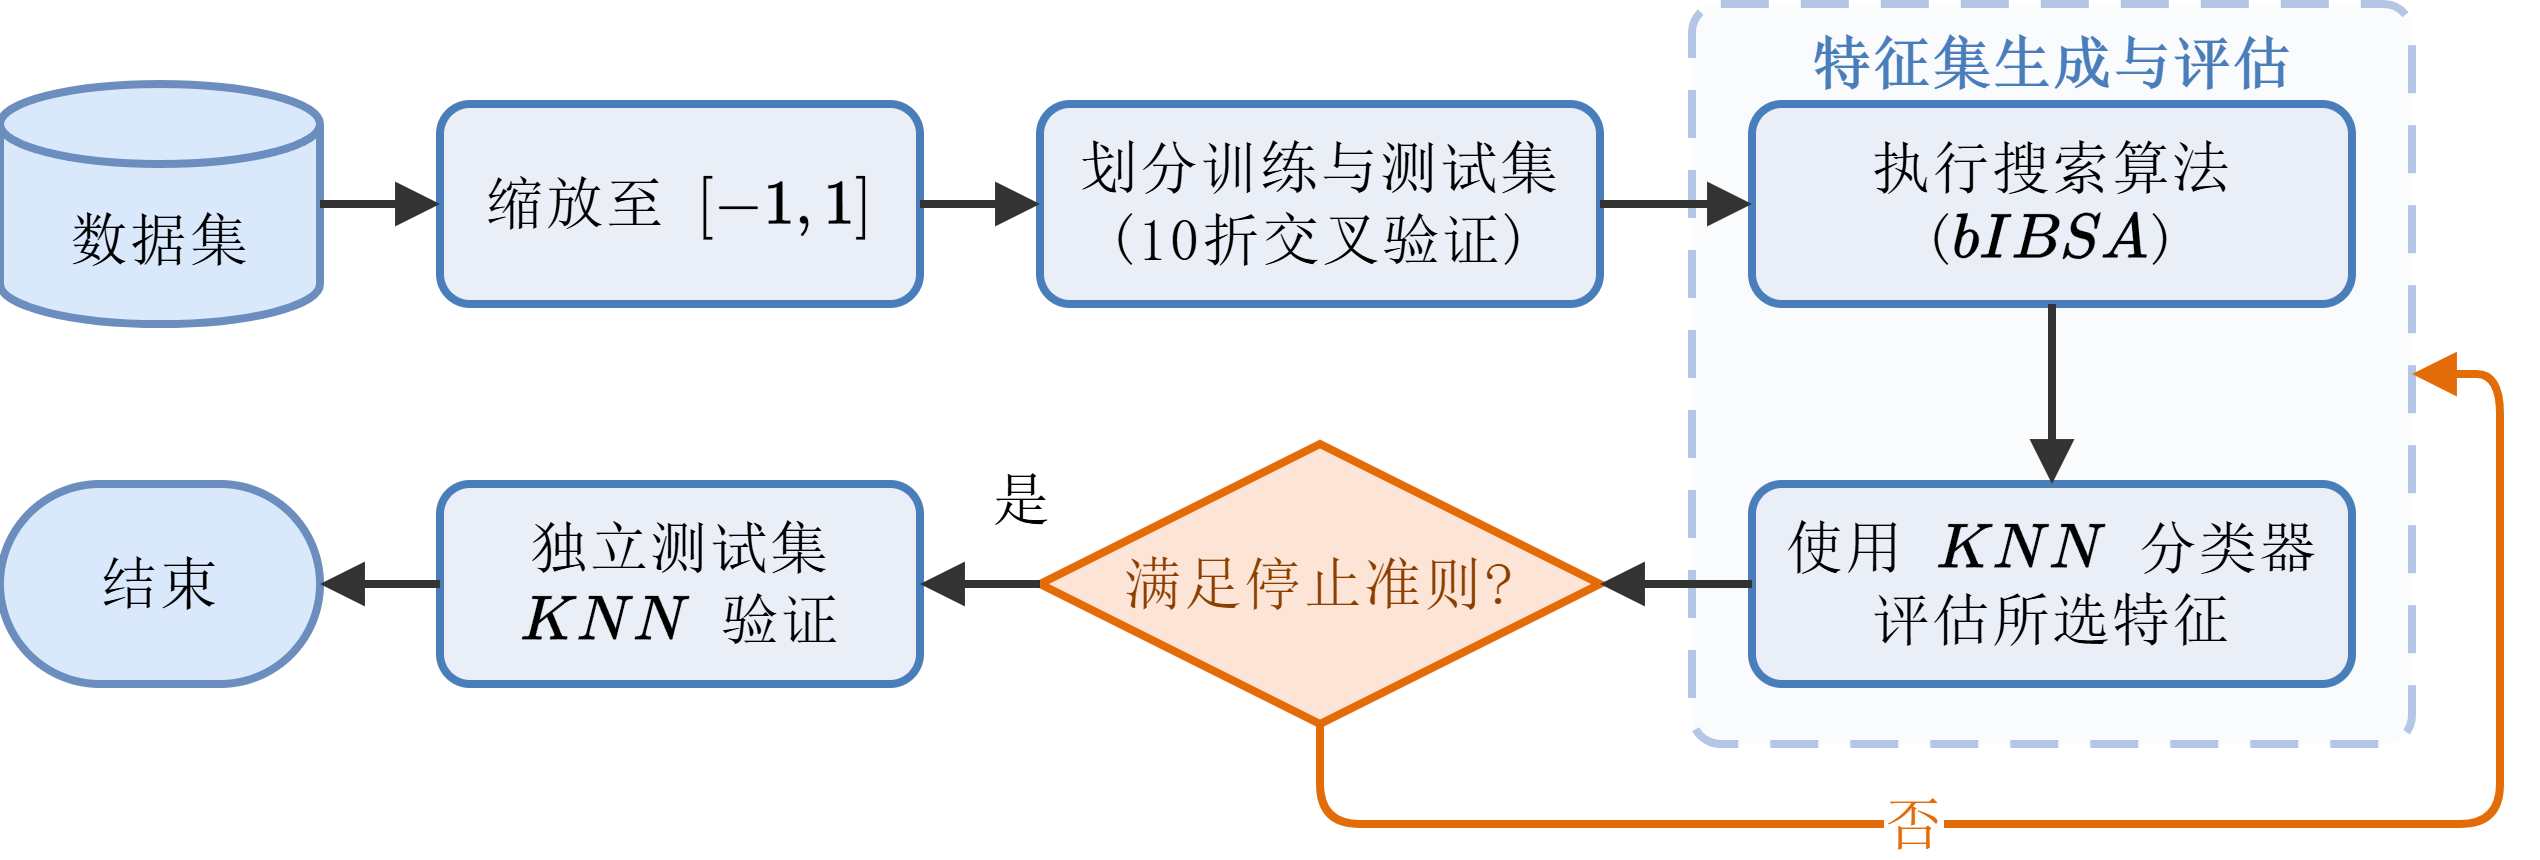
\includegraphics[width=\textwidth]{figures/chapter3/fig3_wrapper_feature_selection.png}
  \bicaption{包裹式特征选择流程}{The wrapper feature selection process}
  \label{fig:wrapper_feature_selection}
\end{figure}


\subsection{计算复杂度分析}

评估IBSA的计算效率时，主要考量指标包括种群规模$(N)$、问题维度$(D)$以及最大迭代次数$(T)$。

IBSA的运行逻辑由初始化、历史库构建、变异映射、杂交演化以及适者生存五个阶段构成。本节重点分析初始化资源占用与精英引导机制的迭代成本。

在系统初始化阶段，算法需要分配空间存储双种群矩阵。这一过程的时间复杂度可表述为$O(N \times D)$。

在精英引导变异策略的迭代循环中，各个环节的贡献不同。历史库的选择主要涉及标志位的判断，计算负载极低，通常在复杂度分析中忽略。

变异与交叉算子是搜索效能的核心。在此阶段，算法需根据适应度排名划分精英与普通层级，排序过程引入了$O(\log N)$的开销。随后，差异化变异在整个演化周期内产生了约$O(T \times N \times D)$的计算流。

最后，生存竞争阶段基于贪婪准则进行适应度判别，在时间尺度上贡献了约$O(T \times N)$的复杂度。

综合分析表明，IBSA的总计算复杂度可表达为$O(N \times D + \log N + T \times N \times (D+1))$。这说明改进策略在提升性能的同时，并未引入超出线性增长范围的额外负担，算法具有良好的可扩展性。


\section{IBSA及bIBSA的实验研究}

为了全面验证改进方案的有效性，本节开展了由标准连续函数测试与实际医学特征筛选组成的实验。其中，连续函数测试用于验证改进策略对搜索性能的增益，医学数据集实验则侧重考察算法在离散工程任务中的泛化表现。

\subsection{实验设置}

全局优化实验采用IEEE CEC 2017基准函数评估IBSA的性能。本文首先分析算法在代表性函数上的探索率、开发率及多样性变化，随后将IBSA与12种基础元启发式算法及11种改进算法进行对比。所有对比算法均采用文献推荐的原始参数，统一设置种群规模为30、维度为30、最大评估次数为300,000，并独立运行30次。结果以平均值和标准差呈现，并结合Wilcoxon秩和检验与Friedman检验分析统计显著性。实验在MATLAB R2018a环境下执行。

全局优化实验的对比算法包括BSA、SMA、DE、PSO、GSA、BA、SCA、CS、WOA、GWO、MFO和HHO等。

\begin{table}[H]
\centering
\bicaption{参与算法的参数设置}{Parameters setting for involved algorithms}
\begin{tabular*}{\textwidth}{@{\extracolsep{\fill}}ll@{}}
\toprule
Algorithm & Other parameters \\ 
\midrule
BSA & $F=3\ \times randn;\ mixrate=1\ $ \\ 
SMA & $z\ =0.03$ \\ 
DE & $Beta_{min}\ =\ 0.2;\ Beta_{max}\ =\ 0.8;\ CR\ =\ 0.2$ \\ 
PSO & $c_1=2;\ c_2=2;\ v_{Max}=6$ \\ 
GSA & $G_0\ =\ 100;\ \alpha\ =\ 20;\ final\_per\ =\ 2$ \\ 
BA & $a=0.5;\ r\ =-0.5$ \\ 
SCA & $a=2$ \\
CS & $m\ =\ 10;\ P_\alpha\ =\ 0.25$ \\
WOA & $a=\left[0,2\right]$ \\
GWO & $a=\left[2,0\right]$ \\
MFO & $a=2;\ b=1$ \\
HHO & $C\ =\ \left[0,2\right];\ E=\left[-2,2\right]$ \\ 
\bottomrule
\end{tabular*}
\end{table}

特征选择实验选取12个UCI医学数据集，并与BMFO、BGWO、BGSA、BPSO、BALO、BBA、BSSA和BWOA进行比较。种群规模设为20。为确保评估公平，采用10折交叉验证和KNN（$K=5$）分类器，最终对比平均适应度、平均错误率、平均特征数及运行时间。

\begin{table}[H]
\centering
\bicaption{控制参数设置}{Setup of control parameter}
\begin{tabular*}{\textwidth}{@{\extracolsep{\fill}}ll@{}}
\toprule
Algorithm & Other parameters \\ 
\midrule
BMFO & $a=2;\ b=1$ \\ 
BGWO & $a=\left[0,2\right]$ \\ 
BGSA & $w_{Max}\ =\ 20;\ w_{Min}\ =\ 1\text{e-}10\ $ \\ 
BPSO & $Max=0.9;\ Min=0.4\ $ \\ 
BALO & None \\ 
BBA & $a=0.5;\ r=0.5$ \\ 
BSSA & $a=2$ \\ 
BWOA & $a\ =\ \left[0,2\right]$ \\ 
\bottomrule
\end{tabular*}
\end{table}

\subsection{特征选择数据描述}

为验证算法在离散问题中的表现，本节利用bIBSA开展特征选择实验。从UCI数据库中选取的12个医学数据集维度范围为326至12,601，涵盖了高维数据场景，能充分检验算法的搜索能力。

这些数据集涵盖了脑肿瘤诊断、中枢神经病变以及多种癌症的病理分析。类别数从2类到7类不等。数据规模与特征维度的显著差异，为评估算法应对“维度灾难”和小样本学习挑战的鲁棒性提供了理想环境。

\begin{figure}[htbp]
  \centering
  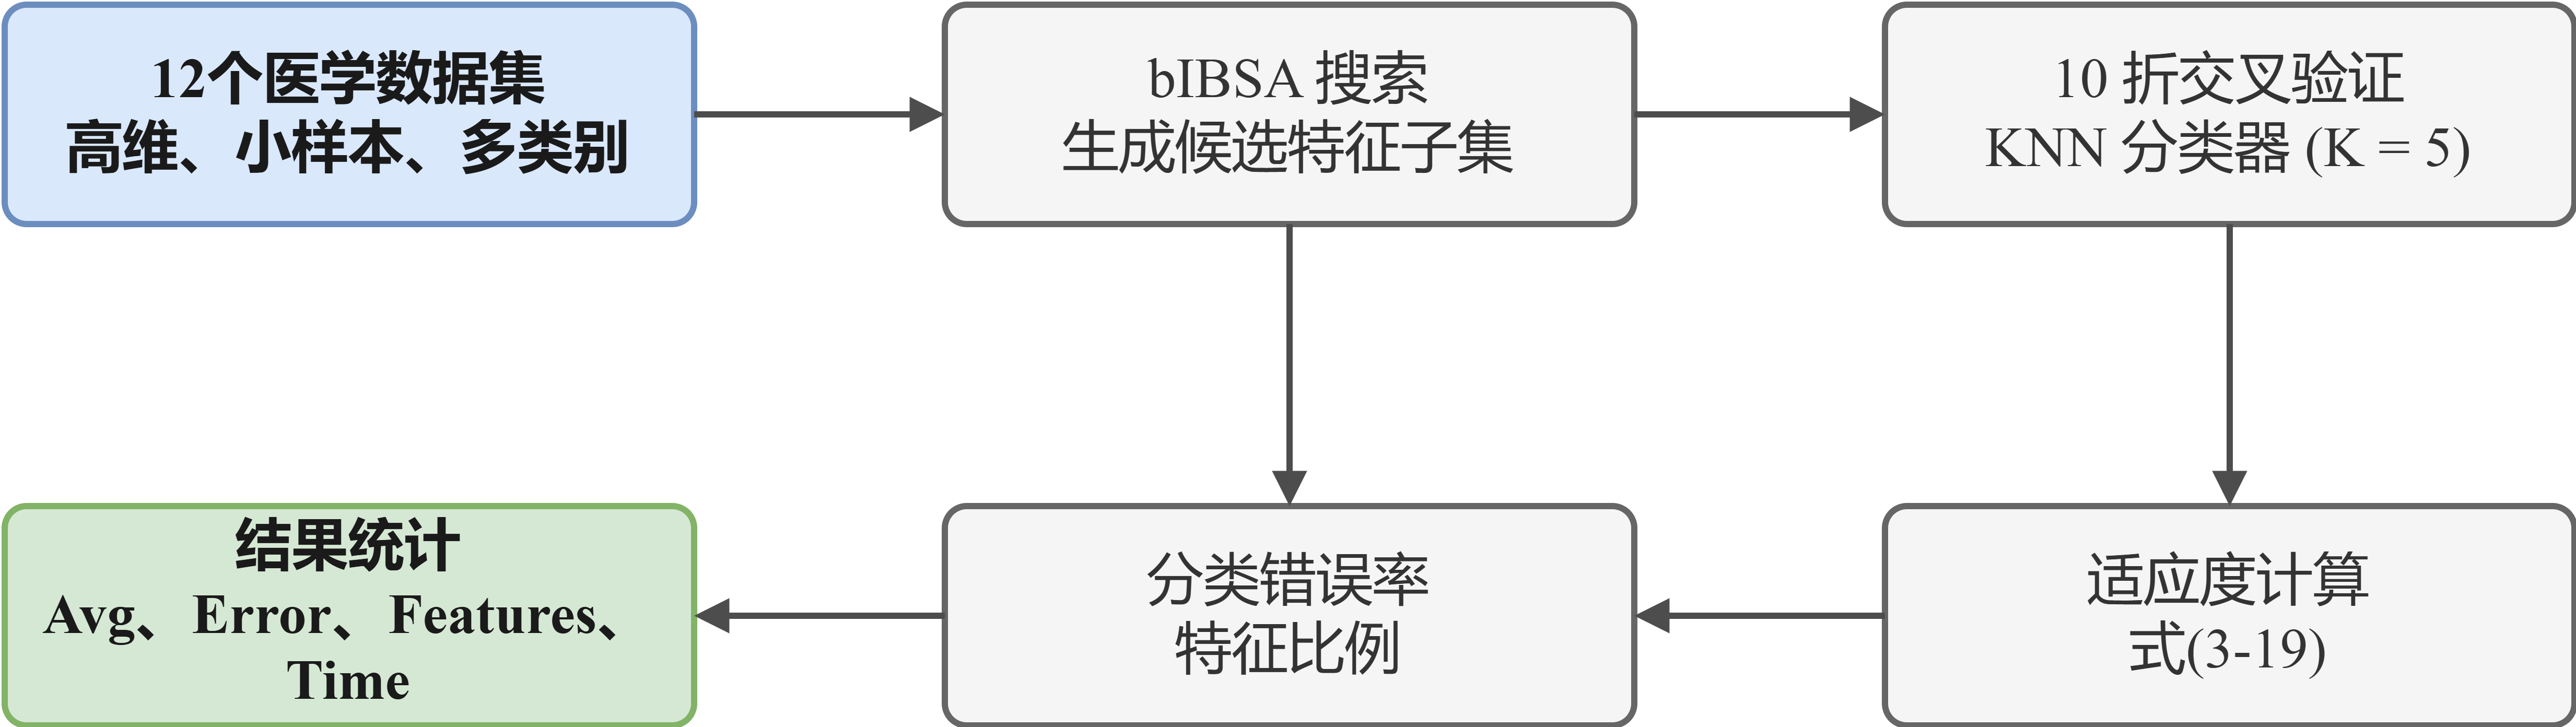
\includegraphics[width=0.88\textwidth]{figures/chapter3/IBSA_fs_evaluate_flowchart_refined.drawio.png}
  \bicaption{医学特征选择实验评估链路}{Evaluation pipeline of the medical feature selection experiments}
  \label{fig:ibsa_fs_pipeline}
\end{figure}

图\ref{fig:ibsa_fs_pipeline}展示了特征选择的评估链路。对于每个特征子集，结合10折交叉验证和KNN分类器估计错误率，计算其适应度并进行多维度比较。

\begin{table}[H]
\centering
\bicaption{所用数据集描述}{Description of the datasets used}
\begin{tabular*}{\textwidth}{@{\extracolsep{\fill}}lccc@{}}
\toprule
Dataset & Samples & Features & Classes \\ 
\midrule
Brain\_Tumor1 & 90 & 5920 & 5 \\ 
Brain\_Tumor2 & 50 & 10367 & 4 \\ 
CNS & 60 & 7130 & 2 \\ 
Colon & 62 & 2001 & 2 \\ 
DLBCL & 77 & 5470 & 4 \\ 
Leukemia & 72 & 7131 & 2 \\ 
Leukemia1 & 72 & 5328 & 5 \\ 
Leukemia2 & 72 & 11225 & 3 \\ 
Lung\_Cancer & 203 & 12601 & 3 \\ 
penglung & 73 & 326 & 7 \\ 
Prostate\_Tumor & 102 & 10509 & 2 \\ 
SRBCT & 83 & 2390 & 4 \\ 
\bottomrule
\end{tabular*}
\end{table}

\subsection{实验结果与分析}

本节首先呈现IBSA在CEC 2017基准函数上的优化结果，随后报告bIBSA在医学数据集上的特征选择表现。

\subsubsection{全局优化实验}

在全面测评之前，本节先选取了六个具代表性的CEC测试函数（F3、F4等），从搜索平衡性、多样性衰减以及收敛特性三个方面对比IBSA与基准 BSA。测试函数涵盖了单峰、多峰、混合及组合拓扑空间。

实验结果显示，IBSA在处理单峰问题时具备更敏锐的收敛精度；在面对拓扑复杂的组合函数时，则能通过动态调节机制维持种群多样性，有效规避局部极值。相比原生BSA，改进后的机制在各类场景中均实现了更平稳的搜寻力度切换，产出的解质量更高，验证了改进策略的有效性。

\begin{figure}[htbp]
  \centering
  \includegraphics[width=\textwidth]{figures/chapter3/fig4_balance_and_diversity.png}
  \bicaption{(a) 函数三维图, (b) IBSA平衡分析, (c) BSA平衡分析, (d) 算法多样性分析, (e) IBSA与BSA收敛曲线}{(a) 3D plot of functions, (b) balance analysis of IBSA, (c) balance analysis of BSA, (d) diversity analysis of algorithm, (e) convergence curve of IBSA and BSA}
  \label{fig:balance_and_diversity}
\end{figure}


上述分析显示，精英引导策略通过自适应调控参数，使IBSA在不同类型函数下均能实现稳定的探索-开发切换。


\FloatBarrier

首先，将IBSA与基础元启发式算法进行比较。

实验数据详细展示了各算法在CEC 2017基准集上的均值、标准差及Friedman排名。从整体看，IBSA在F1、F6等十余个函数上取得了最优结果，并在多数其余函数中名列前茅。特别是在搜寻难度大的混合与组合函数中，IBSA表现出明显的优势，说明改进机制在平衡搜索广度与挖掘深度方面非常有效。

Friedman检验也印证了这一结论。IBSA的平均排名为1.7586，显著优于BSA（3.1379），整体优势见图\ref{fig:friedman_ranking_basic}。

... % Remaining content omitted as requested

\section{本章小结}

针对原生回溯搜索算法在精英引导方面的不足，本章提出了精英引导变异策略，并衍生出二值化算法bIBSA。通过引入精英变异核、自适应扰动向量以及停滞感知的动态切换机制，新模型实现了探索广度与开发深度的有效协同。

实验结果表明，IBSA在CEC 2017全场景测试中展现出卓越的寻优性能，特别是在复杂问题下的稳定性尤为突出。同时，在医学特征选择任务中，bIBSA在大幅压缩特征空间的同时保持了业内领先的分类精度。研究表明，所提出的精英引导范式为处理现代大规模组合优化问题提供了一种有效路径。

\endinput % Omit supplementary tables.


%%% Chapter 4: SBO - Status-based Optimization Algorithm
% Chapter 4: SBO - Status-based Optimization Algorithm
% TODO: Inline [N] citations need conversion to \cite{} with proper .bib entries
%       See the Reference section at the end of SBO_latex/main.tex for the full list.

\chapter{基于状态的优化算法}
\label{chap:sbo}

\section{引言}

现代优化问题日益增长的复杂性对传统确定性方法提出了远超其能力范围的挑战\cite{sbo_ref1}。虽然这些传统方法对于简单的线性问题是有效的，但它们在面对现实世界挑战中高维、动态且经常混沌的特性时往往显得力不从心\cite{sbo_ref2}。此类问题通常涉及庞大的搜索空间、相互冲突的目标以及不断演变的约束条件\cite{sbo_ref3,sbo_ref4}。这一重大缺陷推动了向元启发式算法（Meta-heuristic Algorithms，MAs）的范式转变，与僵化的确定性技术相比，元启发式算法提供了自适应、随机且具有内在鲁棒性的解决方案\cite{sbo_ref5,sbo_ref6}。与其前身不同，MAs在不确定性环境中表现出色，能够在传统方法失效的情况下持续提供近最优解。如今，采用元启发式算法不仅是有益的，而且对于应对全局优化的复杂性至关重要。

\noindent 

\begin{figure}[htbp]
  \centering
  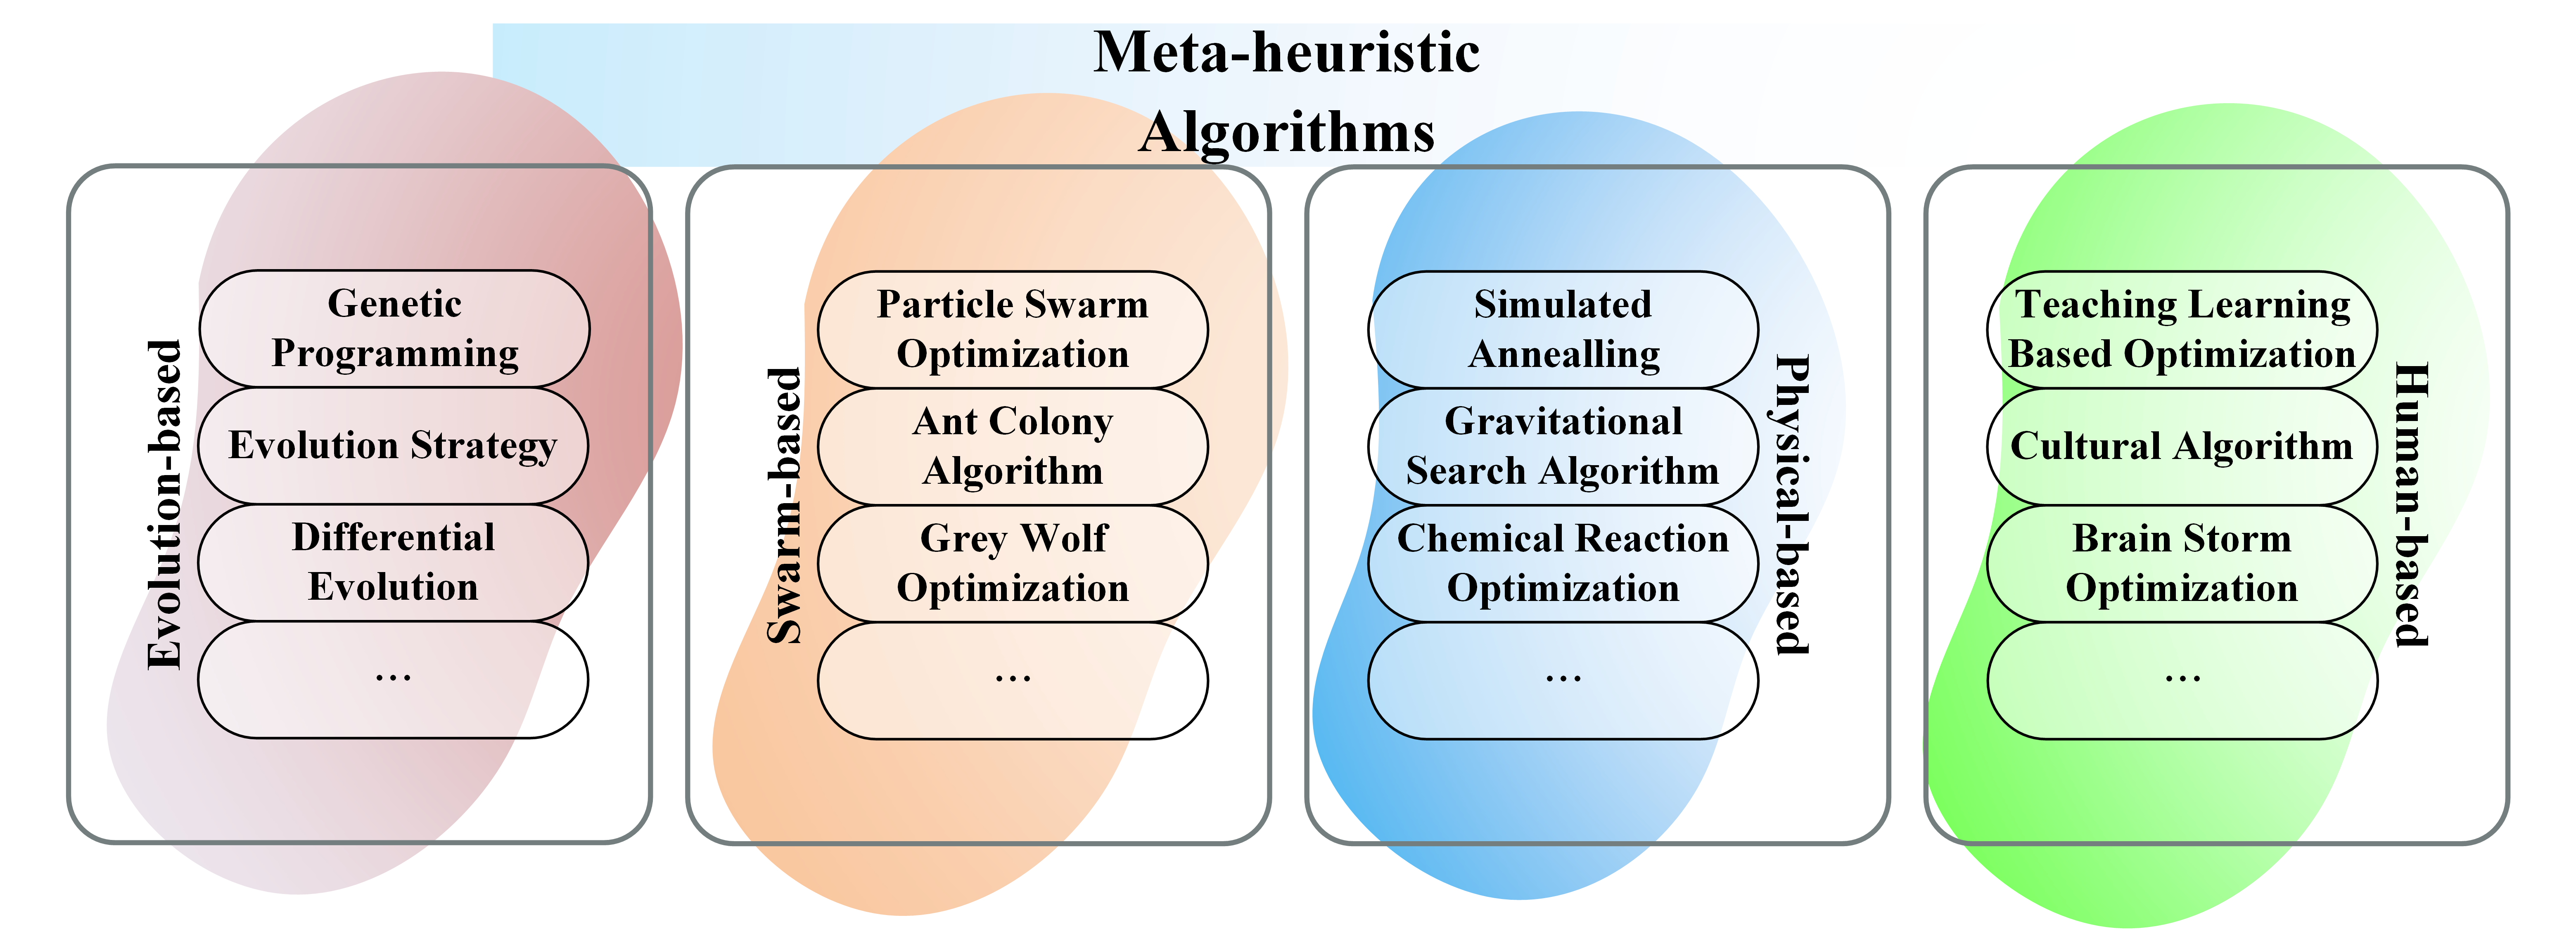
\includegraphics[width=\textwidth]{figures/chapter4/fig01_classification_of_MAs.png}
  \bicaption{四类元启发式算法}{Four types of MAs.}
  \label{fig:sbo_classification_of_MAs}
\end{figure}

鉴于MAs在应对现代优化挑战中的关键作用，有必要探索其多样化的形式，每种形式都采用独特的自然启发策略来应对复杂的问题空间。虽然MAs具有显著的适应性和鲁棒性，但它们通常受到复杂参数调整需求的制约。这一要求阻碍了可扩展性和实际部署，因为最优配置很少是静态的。无论是模拟自然选择的进化算法（Evolutionary Algorithms，EAs）、复制集体行为的群体智能（Swarm Intelligence，SI）模型，还是物理和人类行为启发的启发式算法，所有这些方法都面临这一基本约束，因此对其在动态环境中的实用性提出了质疑。

图1展示了这四个类别，每个类别都具有不同的优势和挑战，进一步说明了需要更好的优化方法。在进一步探讨这一主题时，本文将重点关注参数调整如何影响探索与开发之间的平衡，旨在增强MAs在各种复杂优化场景中的有效性。EAs在MAs的范围内发挥着关键作用，利用自然选择和适者生存的原理。从模仿遗传继承和突变过程的遗传算法（Genetic Algorithm，GA）\cite{sbo_ref7}开始，EAs领域已发展到包括遗传规划（Genetic Programming，GP）\cite{sbo_ref8}、进化策略（Evolutionary Strategies，ES）\cite{sbo_ref9}和差分进化（Differential Evolution，DE）\cite{sbo_ref10}等变体。EAs以其广泛的应用和通过迭代选择、交叉和变异过程寻找全局最优的能力而闻名\cite{sbo_ref11}。尽管具有这些优势，EAs面临一个重大问题：它们对参数设置（即突变率和交叉概率）的调整非常敏感。需要仔细调整这些参数以适应不同的优化环境，这促使研究人员致力于创建自适应和自调整的进化算法\cite{sbo_ref12,sbo_ref13}。这一研究方向旨在简化参数校准，同时提高EAs在解决各种优化问题时的灵活性。

SI算法借鉴了社会性生物中观察到的集体和自组织行为的思想。粒子群优化（Particle Swarm Optimization，PSO）\cite{sbo_ref14}、蚁群优化（Ant Colony Optimization，ACO）\cite{sbo_ref15}和灰狼优化（Grey Wolf Optimization，GWO）\cite{sbo_ref16}等方法体现了这些原理。PSO模拟了鸟群中观察到的动态交互。另一方面，ACO模仿了蚂蚁的路径寻找行为，而GWO则模拟了灰狼的协作狩猎策略。在GWO方法中，虚拟狼群中的每只狼根据alpha、beta和delta狼的影响更新其位置，这三只狼分别代表迄今为止获得的第一、第二和第三最优解。通过重复迭代，狼群逐渐接近潜在的最优解，展示了GWO作为优化技术的有效性\cite{sbo_ref17}。群体智能算法基于这样一个原理运行：一群遵循基本交互规则的简单代理能够共同展现出复杂且全局有效的行为，从而解决复杂的优化问题\cite{sbo_ref18}。通过模拟社会行为，这些算法通过所有搜索代理之间的合作和信息交换，高效地探索问题空间。尽管这些算法具有内在的灵活性和强大的并行搜索能力，但它们面临与参数配置相关的挑战。关键参数设置，包括参与代理的数量、交互规则和收敛准则，在决定算法性能和收敛速率方面起着关键作用\cite{sbo_ref19}。

物理/化学启发方法提供了一种不同的优化途径，利用物理和化学的过程与定律。该类别包括模拟退火（Simulated Annealing，SA）\cite{sbo_ref20}和引力搜索算法（Gravitational Search Algorithm，GSA）\cite{sbo_ref21}等算法。前者受冶金退火启发，后者基于引力和质量相互作用原理。此外，化学反应优化（Chemical Reaction Optimization，CRO）\cite{sbo_ref22}等方法模拟了化学反应中观察到的分子相互作用和能量交换。这些算法因其能够逃避局部最优而受到特别赞誉\cite{sbo_ref23}，这是通过模拟物理和化学系统中存在的自适应和随机行为来实现的。尽管这些算法引入了创新的探索策略，但它们仍然面临与参数选择相关的挑战\cite{sbo_ref24}，这是一个影响探索与开发之间平衡的关键问题，最终影响其找到良好解的能力。

基于人类行为的算法展示了如何将认知过程和社会交互融入元启发式优化框架。例如，教学优化算法（Teaching-Learning-Based Optimization，TLBO）\cite{sbo_ref25}模拟教育环境的动态，文化算法（Cultural Algorithm，CA）\cite{sbo_ref26}反映文化知识的演化和传递，头脑风暴优化（Brain Storm Optimization，BSO）\cite{sbo_ref27}模拟头脑风暴的集体问题解决能力。这些算法因模仿以人为中心的问题解决策略而表现出色，包括从经验中学习、利用记忆以及社会交互的微妙影响\cite{sbo_ref28}。然而，这些算法的性能在很大程度上取决于它们模拟复杂人类行为的准确程度。一个关键问题在于调整控制个体学习和社会动态的参数，这可能极大地影响算法探索搜索空间的能力。

为了改进元启发式方法，本文提出了基于状态的优化算法（Status-based Optimization，SBO），这是一种模拟人类社会地位提升细节的高效算法。SBO的基础深植于看似无形却强大的社会向上流动网络中，其中个体积极寻求与更优秀同伴的联系并向其学习。SBO的设计体现了这种追求卓越、获取有用知识和资源以实现自我提升的自然倾向\cite{sbo_ref29}。

类似于攀登社会阶梯可以带来个人成长和丰富，SBO算法在优化领域模拟了这一进步过程。它将探索阶段视为个体努力进入更高地位圈子的过程，在算法术语中，这相当于搜索解空间中最有前景的区域。随后，开发阶段被视为个体利用在这个高级圈子中获得的机会和联系，类似于对最优解进行精炼以获得最佳性能。因此，SBO算法通过其出色的灵活性和精心设计的框架，将人类通过旨在提升地位的互动来持续改进的努力与系统化的优化方法进行了直接类比。本文的主要贡献总结如下：

\begin{enumerate}
\item  本文提出了SBO，一种模拟人类寻求地位行为和交互的新型MA，为启发式优化提供了新的途径。

\item  SBO算法展现出强大的全局优化能力，其性能通过IEEE CEC 2017测试套件的全面测试得到验证。

\item  SBO算法性能的可靠性通过详细的统计检验得到验证，包括Wilcoxon符号秩检验和Friedman检验。这些检验证实了其优化结果的统计显著性和可靠性。

\item  SBO算法的实用性和有效性在高维特征选择和多阈值图像分割任务中得到进一步验证。这些结果证明了其潜在的灵活性，表明其在各种工程领域的适用性。
\end{enumerate}

本文的结构安排如下：第2节回顾了人类行为启发的元启发式算法，为第3节中SBO的详细阐述奠定基础，该节研究了其概念基础和底层数学模型。第4节对SBO的性能进行了全面的基准测试，而第5节展示了其在现实世界特征选择和多阈值图像分割任务中的应用。最后，第6节总结了主要结果并讨论了潜在的未来研究方向。


\section{文献综述}

优化算法分为两大类型：启发式方法和元启发式方法。启发式算法是利用预设规则或专家知识快速找到足够好的解的专用方法，但它们无法保证找到最优解。它们是针对特定问题定制的，如贪心算法和局部搜索方法。

另一方面，MAs是灵活的问题求解器，管理搜索过程以平衡广泛的探索和集中的改进。与启发式方法不同，元启发式方法无需重大修改即可处理许多不同的问题。它们通常使用随机元素和自调整方法来逃离局部最优，使其更适合处理困难的高维问题。值得注意的是，许多元启发式算法将启发式方法作为其解改进过程的一部分，展示了两种类型之间的联系。

本文将新提出的SBO算法归入元启发式类别，因为它利用受人们追求更高社会地位启发的自适应学习来提高搜索效率。与遵循固定规则的传统启发式方法不同，SBO通过信息共享和资源评估动态调整其搜索策略，增强了探索和开发能力。由于人类行为启发算法在研究中产生了重要影响，本文将重点回顾该领域的关键示例。特别是，TLBO、BSO、政治优化（Political Optimization，PO）和人类心智搜索（Human Mental Search，HMS）作为类人问题求解的典型代表脱颖而出。研究这些算法不仅有助于在现有研究中定位SBO，还展示了人类启发策略在优化领域的发展历程。

TLBO\cite{sbo_ref30}算法是最经典的人类启发元启发式算法之一，模拟课堂的教学-学习过程，不需要算法特定的参数。其简单性催生了各种改进：例如，多目标TLBO（MOTLBO）\cite{sbo_ref31}通过有效地平衡重量和材料强度之间的权衡来优化结构设计；改进的TLBO（ITLBO）\cite{sbo_ref32}已成功应用于配电系统。此外，自适应混合自学习TLBO（SHSLTLBO）\cite{sbo_ref33}通过引入自适应学习策略来增强基本算法，将搜索聚焦于有前景的区域。

BSO算法\cite{sbo_ref34}模拟人类的头脑风暴过程，通过迭代的想法交流产生多样化的解。增强版本如最优识别框架与BSO的融合（OIF-BSO）\cite{sbo_ref35}通过最优识别机制改进搜索方向，而高级基于网格的BSO（AGBSO）\cite{sbo_ref36}则采用替代搜索模式和基于网格的算子来更好地应对不确定环境。

PO\cite{sbo_ref37}借鉴了人类政治系统的复杂性，使用多代理框架，其中竞争和合作交互驱动最优解的搜索。其有效性在改进的PO（IPO）\cite{sbo_ref38}等变体中得到进一步提升，该变体添加了精密的政治策略以提高性能；量子Nelder-Mead PO（QNMPO）\cite{sbo_ref39}则将量子原理与政治优化相结合以增强能源系统中的性能。

HMS算法\cite{sbo_ref40}捕获了人类问题解决中固有的认知和决策过程。全局最优引导HMS与随机聚类策略（GBG-HMS-RCS）\cite{sbo_ref41}将全局最优引导与随机聚类相结合，模拟人类的注意力和意识。此外，多聚类选择HMS（MCS-HMS）\cite{sbo_ref42}形成多个认知集群以识别有前景的解区域，这一策略在供应链管理和运输物流等复杂场景中证明是有效的。

综上所述，本节仔细考察了受人类行为不同方面启发的一系列重要算法。TLBO中展示的教学-学习动态、BSO中的团队创造力、PO中的政治策略以及HMS中的思维过程，都将人类行为转化为计算工具。虽然这些人类启发算法在处理复杂问题方面表现良好，但它们也存在一些弱点：

\begin{enumerate}
\item  TLBO不需要参数调整，但收敛速度可能较慢

\item  BSO使用创造性搜索方法，但可能过早收敛

\item  PO可能需要大量计算

\item  HMS通常需要仔细调整才能获得最佳结果
\end{enumerate}

\noindent 与这些算法相比，新提出的SBO算法提供了以下关键改进：

\begin{enumerate}
\item  需要调整的参数更少，使用更加方便

\item  得益于其社会学习方法，在广泛搜索和局部精炼之间取得了更好的平衡

\item  运行时间更快，如本文测试（第4.4节）所示，SBO在运行效率上始终优于其他方法
\end{enumerate}

\noindent 这些优势使SBO更适用于现实世界的复杂优化问题。

本文开发SBO的目的是结合这些人类启发方法的最佳特性，同时克服其局限性。在接下来的章节中，本文将阐述：SBO的灵感来源、其数学工作原理以及应用领域。这将展示SBO如何与其他元启发式方法相匹配，并解决现有方法中发现的问题。


\section{所提基于状态的优化算法}

本节重点介绍SBO算法的阐述，详细说明其数学建模和计算复杂度。


\subsection{SBO的灵感来源}

SBO算法模拟了人类攀登社会阶梯的本质驱动力——一种根植于自我提升需求的行为\cite{sbo_ref43}。这种追求反映了优化的核心目标：迭代精炼。就像人们通过与成功同伴建立联系来获得优势一样\cite{sbo_ref44}，SBO代理从高性能解中学习以提高搜索效率。

\noindent 认知科学和行为经济学的研究证实，向高地位个体学习可以改善复杂场景中的问题求解。SBO将此转化为计算术语，创建了一种集体智能，其中：

\begin{enumerate}
\item  代理共享知识（类似人类网络）

\item  多样化策略自然涌现

\item  系统平衡探索与开发
\end{enumerate}



简而言之，SBO的工作方式如下：

\begin{enumerate}
\item  \textbf{精英接触（探索）}

\begin{enumerate}
\item  代理跟随最优个体以发现有前景的区域

\item  类似于在社会层级中寻找导师
\end{enumerate}

\item  \textbf{资源阶段（开发）}

\begin{enumerate}
\item  \textbf{获取}：从精英中收集信息

\item  \textbf{评估}：像专业人员提升技能一样精炼解
\end{enumerate}
\end{enumerate}



已有多种受人类地位驱动的社会行为和教育交互启发的优化算法成功解决了复杂问题。基于人类行为的优化（Human Behavior-Based Optimization，HBBO）算法\cite{sbo_ref45}模拟了合作、竞争、模仿和社会学习等集体人类行为。HBBO通过模仿、创新和协作等机制平衡社会学习与个体创造力，使其适用于动态或多目标问题。

类似地，教育竞争优化器（Educational Competition Optimizer，ECO）\cite{sbo_ref46}模拟了竞争性学习环境，其中解相互竞争并向最优个体学习，由最优解引导，类似于教师。这种方法促进了快速收敛和对约束优化场景的适应性，展示了其在学术成绩建模和博弈论等应用中的效率。



通过形式化寻求地位的行为，SBO在以下方面优于前述算法：

\begin{enumerate}
\item  平衡全局/局部搜索

\item  减少手动参数调整

\item  可扩展至高维问题
\end{enumerate}


\subsection{SBO的数学建模}

受人类寻求地位行为的启发，SBO算法将优化框架化为个人和社会发展过程。它首先生成两个多样化的代理种群——代表来自不同社会背景的个体——然后通过模仿向社会精英寻求指导的过程来进化。

关键阶段如下：

\begin{enumerate}
\item  \textbf{精英追求}：代理识别并向高性能解（"导师"）移动

\item  \textbf{资源获取}：获得有价值的信息（社会资本）

\item  \textbf{策略整合}：代理批判性地评估并仅采用最有利的改进
\end{enumerate}

这反映了人们如何：

\begin{enumerate}
\item  通过向成功同伴学习来\textbf{社会进步}

\item  \textbf{选择性采纳}能提升自身地位的行为

\item  通过积累优势来\textbf{系统性攀升}层级
\end{enumerate}

算法最终通过巩固这些改进来提供最优解——在数学上代表地位成就的顶峰。（完整的数学细节将在后续部分展开。）

\noindent 
\subsubsection{3.2.1 初始化}

初始化阶段通过生成两个种群$X^1$和$X^2$奠定了SBO算法的基础。在该模型中，每个索引$i$对应一个唯一的家庭，其中$X^1$和$X^2$中相同索引的个体代表具有不同知识水平和社会地位的家庭成员。这种双种群设计确保每个家庭至少由两个个体代表，从而捕获家庭内部的多样性，并在算法迭代时能够动态更新精英成员。

\begin{equation}
\label{sbo_eq_1}
X^1,\ X^2={\left[ \begin{array}{c}
x_1 \\ 
\vdots  \\ 
x_2 \\ 
\vdots  \\ 
x_N \end{array}
\right]}_{N\times D}={\left[ \begin{array}{ccccc}
x_{1,1} & \cdots  & x_{1,j} & \cdots  & x_{1,N} \\ 
\vdots  & \ddots  & \vdots  & \ddots  & \vdots  \\ 
x_{i,1} & \cdots  & x_{i,j} & \cdots  & x_{i,D} \\ 
\vdots  & \ddots  & \vdots  & \ddots  & \vdots  \\ 
x_{N,1} & \cdots  & x_{N,j} & \cdots  & x_{N,D} \end{array}
\right]}_{N\times D}
\end{equation}



每个个体的状态由式~\eqref{sbo_eq_2}定义：

\begin{equation}
\label{sbo_eq_2}
x_{i,j}=U\left(lb_j,\ ub_j\right)
\end{equation}

其中$x_{i,j}$是第$ith$个个体的第$jth$个决策变量，$D$是决策变量的数量，$lb_j$和$ub_j$分别是下界和上界。两个种群在$N\times D$矩阵上的均匀初始化建立了问题的维度特性，并确保了多样化的起始点。

初始化后，通过选择过程识别每个家庭的精英成员，以形成精英种群$X^e$。具体而言，对于第$ith$个家庭，

\begin{equation}
\label{sbo_eq_3}
\begin{array}{c}
x^e_i=\left\{ \begin{array}{c}
x^1_i\ \ \ \ \ \ \ \ \ \ \ \ \ \ \ \ \ \ \ \ if\ fobj\left(x^1_i\right)<fobj\left(x^2_i\right)\ \ \ \ \ \ \ \ \ \ \ \ \ \ \ \ \ \ \  \\ 
x^2_i\ \ \ \ \ \ \ \ \ \ \ \ \ \ \ \ \ \ \ \ \ \ \ \ \ \ \ \ \ \ \ \ otherwise\ \ \ \ \ \ \ \ \ \ \ \ \ \ \ \ \ \ \ \ \ \ \ \ \ \ \ \ \ \ \ \ \ \  \end{array}
\right.\# \end{array}
\end{equation}

其中$fobj\left(\cdot \right)$是目标函数。

这种双种群方法不仅仅是在每个群体中找到最优表现者——它反映了现实世界的社会流动性，其中进步取决于个人能力和战略联系。普通个体$x_i$与其精英对应体$x^e_i$之间的交互模拟了现实世界中以地位为导向的社会网络，说明了精英人物如何促进家庭单元内部和之间的进步与资源共享。

\noindent 
\subsubsection{3.2.2 精英接触}

在精英接触阶段，SBO算法复制了人类社会地位结构的复杂动态，以增强对最优解的搜索。该阶段模拟了个体向高地位导师——算法中的精英代理——寻求指导以加速其进步的过程。与孤立的家庭框架不同，这种进步超越了自包含的群体，通过在不同社会单元之间建立互联来创建更具适应性和鲁棒性的搜索机制。

为模拟这一行为，SBO算法使用轮盘赌选择方法\cite{sbo_ref47}从种群子集中选择一个个体。该子集代表不同家庭中最成功的成员。这种概率选择过程确保个体不仅仅依赖单一的主导同伴，而是考虑多个有影响力的代理，反映了人类社交网络中不可预测但具有战略性的特征。

被选中的个体，记为$x^e_r$，与种群中的最优个体$x_b$共同定义了一个高地位圈子——解空间中一个比喻性的但具有计算意义的区域，代理们旨在融入其中。这种社会流动性的动态表示确保个体系统性地向搜索空间中更有前景的区域过渡。

为了在数学上表达这一行为，式~\eqref{sbo_eq_4}和图2描述了高地位圈子内个体$x_i$的生成——定义了解空间中的有前景区域。这个高地位圈子代表一个自适应区域，个体在其中向更优解导航，平衡结构化进步和探索性随机性。个体的移动由以下公式控制：

\begin{equation}
\label{sbo_eq_4}
x_{i'}=\left\{ \begin{array}{cc}
\left(1-w_1-w_2\right)\times x_i+w_1\times x^e_r+w_2\times x_b & if\ rand<w_3 \\ 
w_4\times \left(\left(1-w_1-w_2\right)\times x_i+w_1\times x^e_r+w_2\times x_b\right) & Otherwise \end{array}
\right.
\end{equation}

其中$x_i$代表种群中的第$ith$个个体，$x_{i'}$表示下一次迭代，$x^e_r$是通过轮盘赌方法从$X^E$种群中选择的精英个体，$x_b$是迄今为止找到的最优解。式~\eqref{sbo_eq_4}中的移动策略确保个体受到自身位置、高性能同伴和已知最优解的影响。

参数$w_1$和$w_2$使用$randn$生成，提供正态分布的随机性来加权$x_i$、$x^e_r$和$x_b$的贡献。这些值在确保移动保持在逻辑边界内的同时引入随机性，促进了在解空间中受控但多样化的搜索。

相比之下，$w_3$和$w_4$是设计参数，动态调整高地位圈子对探索和开发的影响。$w_3$的计算方式为：

\begin{equation}
\label{sbo_eq_5}
\begin{array}{c}
w_3={\mathrm{tanh} \left({\left(\frac{\sqrt{\left|MaxFEs-randn\times FEs\right|}}{i}\right)}^{\frac{FEs}{MaxFEs}}\right)\ }\# \end{array}
\end{equation}

其中$MaxFEs$表示最大函数评估次数，$FEs$是当前评估次数，$i$是个体的索引。这一公式允许$w_3$随着优化进程的推进而自适应调整，决定应用标准更新规则还是更随机化的搜索。

如果$rand\ge w_3$，则使用式~\eqref{sbo_eq_4}中的第二种公式，其中$w_4$作为缩放因子，在$[-w_3,w_3]$之间生成均匀分布的随机数。这种机制通过实现步长调整来增加探索多样性，特别是在逃离局部最优时。

\begin{equation}
\label{sbo_eq_6}
w_4=unifrnd\left(-w_3,\ w_3\right)
\end{equation}



\begin{figure}[htbp]
  \centering
  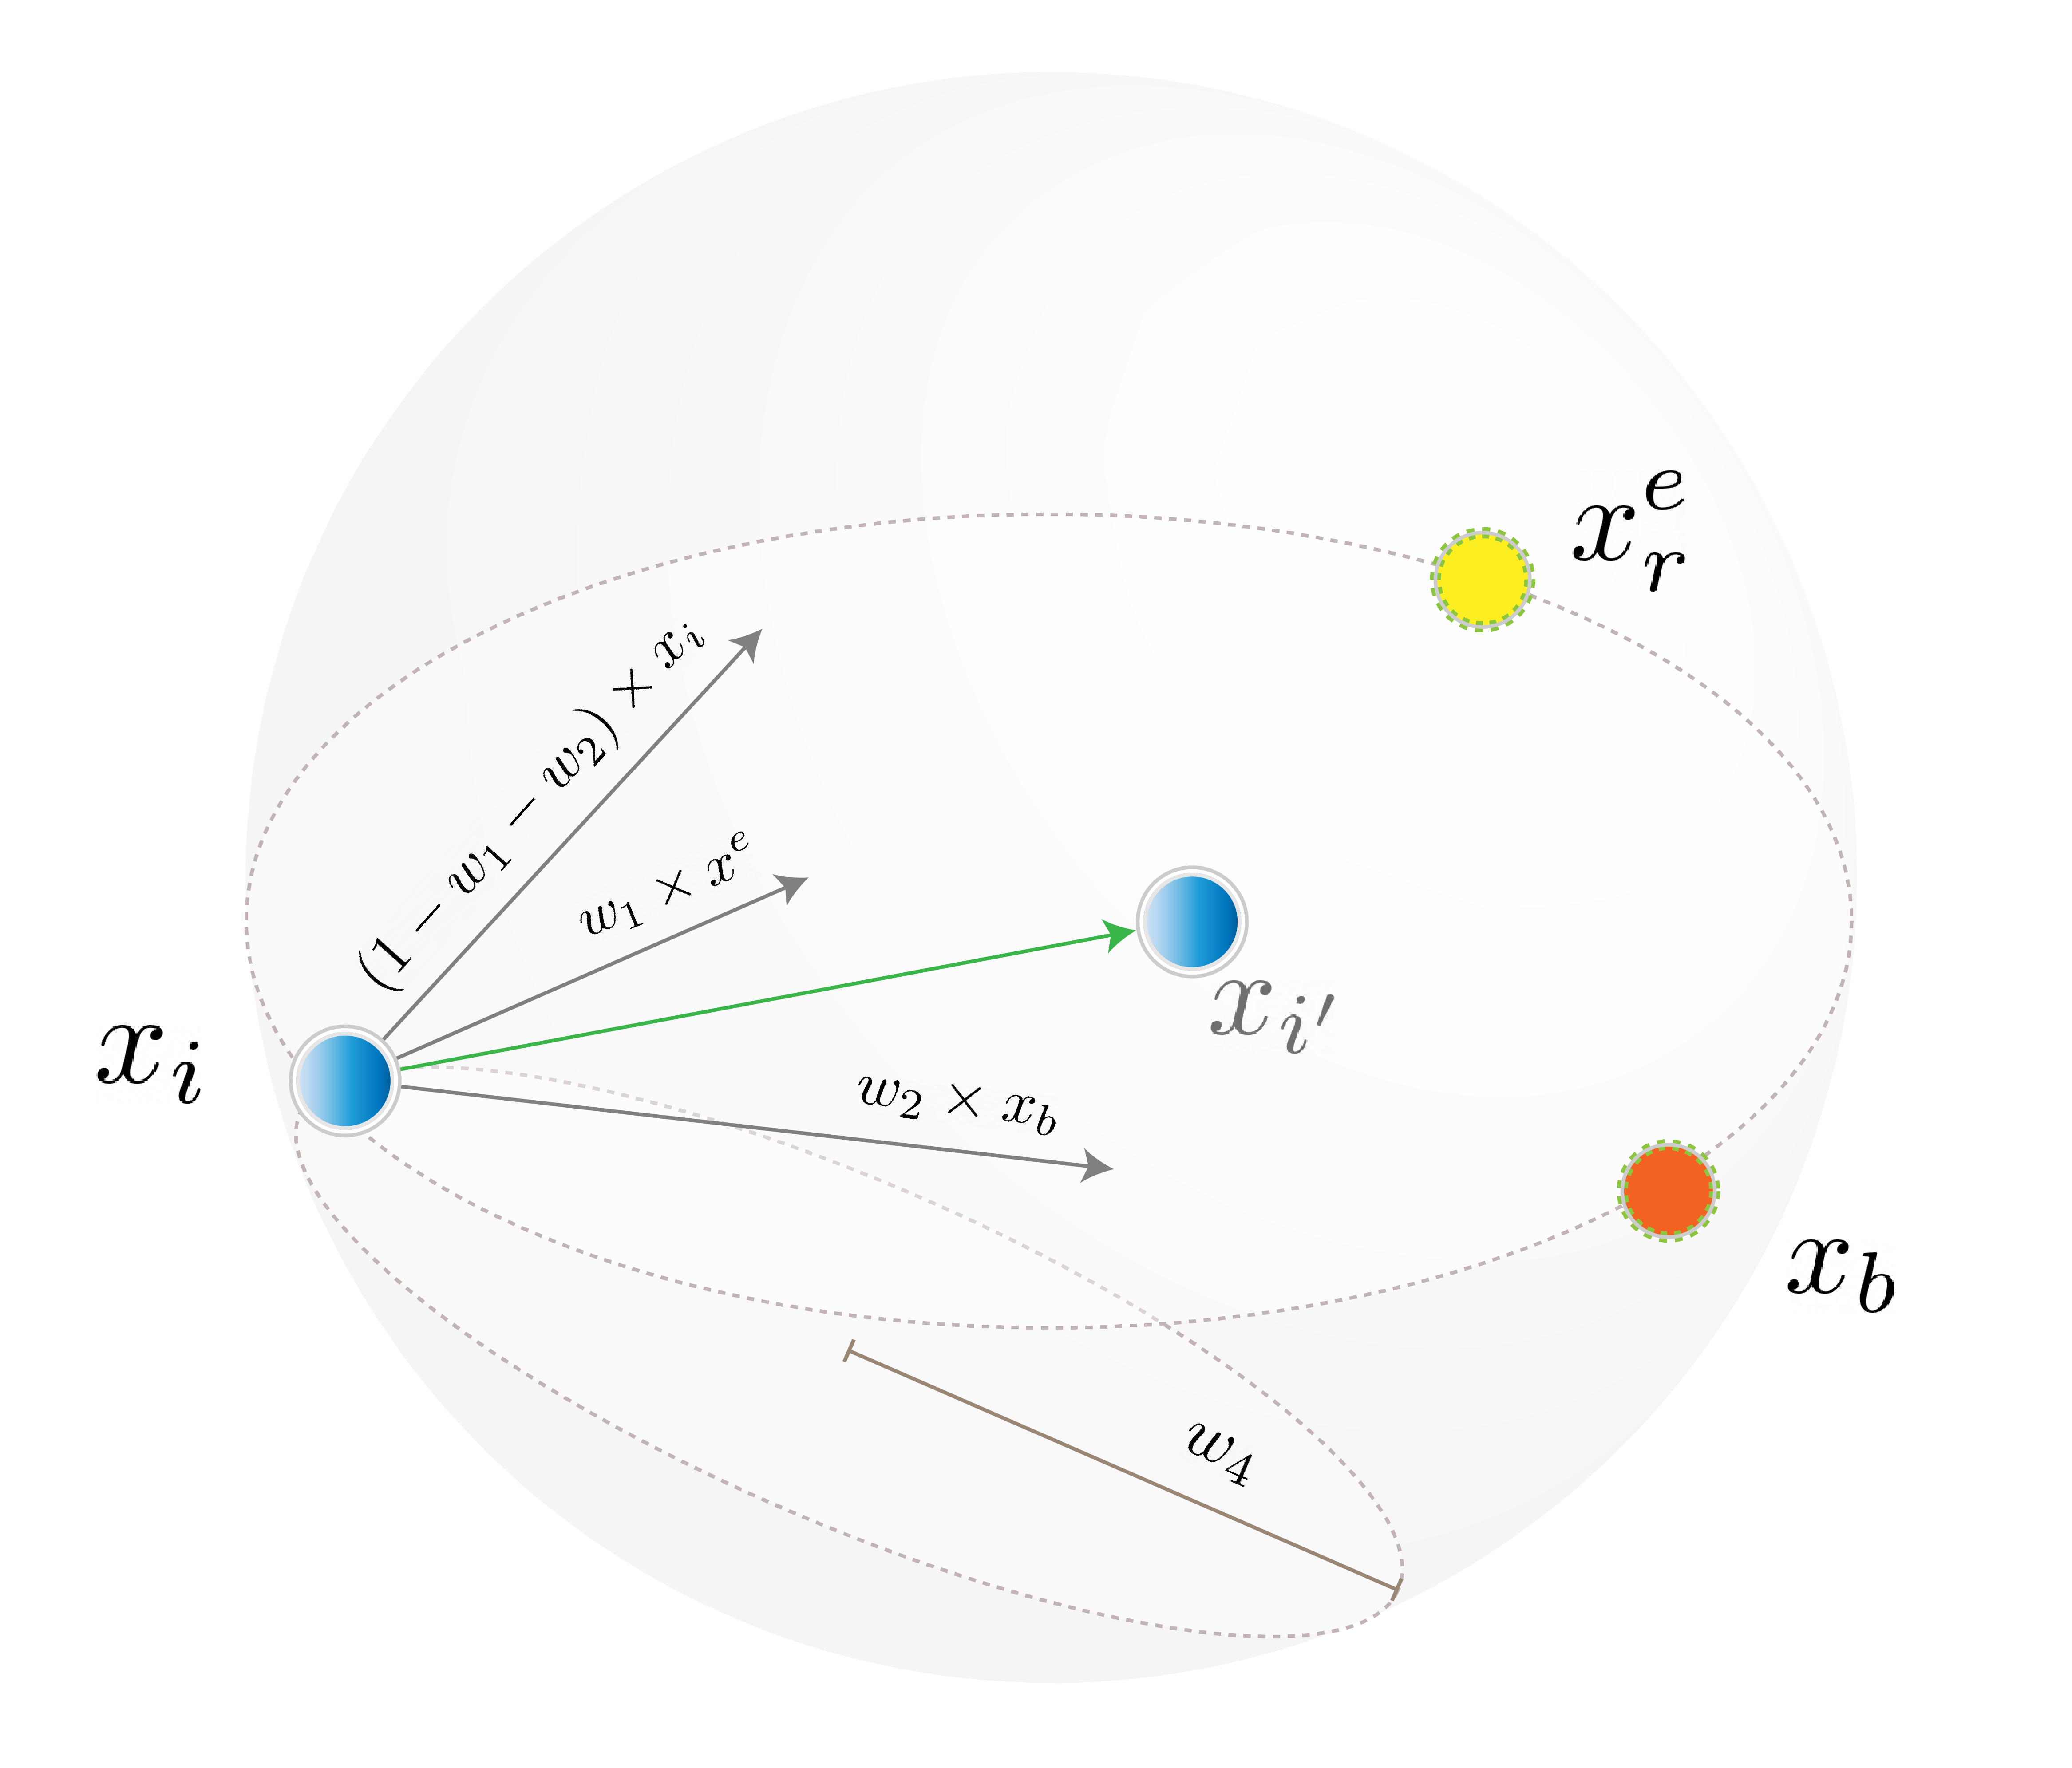
\includegraphics[width=\textwidth]{figures/chapter4/fig02_elite_engagement.png}
  \bicaption{SBO的精英接触阶段}{Elite Engagement phase of SBO.}
  \label{fig:elite_engagement}
\end{figure}



通过整合这些组件，SBO算法反映了现实世界的决策过程——个体追随成功同伴的同时战略性地探索非常规路径以优化结果。式~\eqref{sbo_eq_4}中的初始公式战略性地计算高地位圈子内的最优位置，反映了个体如何获得进入有影响力网络的机会以获得更好的前景。通过进化计算，解逐步改进，向搜索空间中更有前景的区域移动。

相比之下，第二种公式引入了范围为$[-w_3,w_3]$的随机缩放因子，允许算法探索直接有前景区域之外的空间。这一特性防止了过早收敛，同时使SBO能够在未探索区域中发现潜在的更优解。这种平衡反映了人类的决策过程。人们有时会偏离既定路径，无论是通过职业变更还是创新尝试，来寻找传统方法可能忽略的机会。

通过结合结构化学习和探索灵活性，SBO实现了开发和探索之间的最佳平衡。这使算法能够有效适应复杂的优化环境。由此产生的方法在保持跨不同问题鲁棒性的同时提高了解的质量，证明了SBO的高性能优化能力。

\noindent 
\subsubsection{3.2.3 资源获取}

资源获取阶段在从探索到开发的转换中至关重要，通过获取和利用有价值的见解——如同人类网络中的社会资本。在该阶段，为$X$种群中的所有个体创建一个$flag$向量，初始设为1以表示暂时的地位相关成功。该标志稍后在资源评估阶段更新，作为每个个体地位改善效果的动态指标。

资源获取机制根据地位相关的成功情况而有所不同。对于社会上成功的个体，资源通过平均两个来源的输入来选择性获取：一个来自同一家庭单元的精英个体，另一个来自种群中的整体最优个体。这一过程由以下公式描述：

\begin{equation}
\label{sbo_eq_7}
x^s_{i,j_1}=\frac{x^e_{i,j_2}+x_{b,j_3}}{2}
\end{equation}

其中$j_{idx}=randi\left(D\right)$（$idx=1,2,3$），反映了家庭内部和外部精英影响的融合。

相反，社会上不成功的个体仅依赖家庭资源。其资源更新遵循以下公式：

\begin{equation}
\label{sbo_eq_8}
\begin{array}{cc}
x^s_{i,j}=x^e_{i,j} & if\ m_j=1 \end{array}
\end{equation}

其中行向量$m$初始为零，在社会交互之前通过以下方式更新：

\begin{equation}
\label{sbo_eq_9}
m\left(u\left(1:ceil\left(rand\times D\right)\right)\right)=1
\end{equation}

其中$u=randperm(D)$提供决策变量索引的随机排列。

如图3所示，该阶段将种群引导至解空间中有前景的区域以最大化开发。

\begin{enumerate}
\item  图3(a)\textbf{：}成功个体通过利用来自更高地位代理的资源来精炼其位置

\item  图3(b)\textbf{：}困难个体通过家庭资源重新定位
\end{enumerate}

\noindent

该算法复制了地位驱动的社会动态，其中资源丰富的个体自然地吸引更多机会，系统性地引导种群走向更优解，从而显著提升开发能力并增强整体优化性能。



\begin{figure}[htbp]
  \centering
  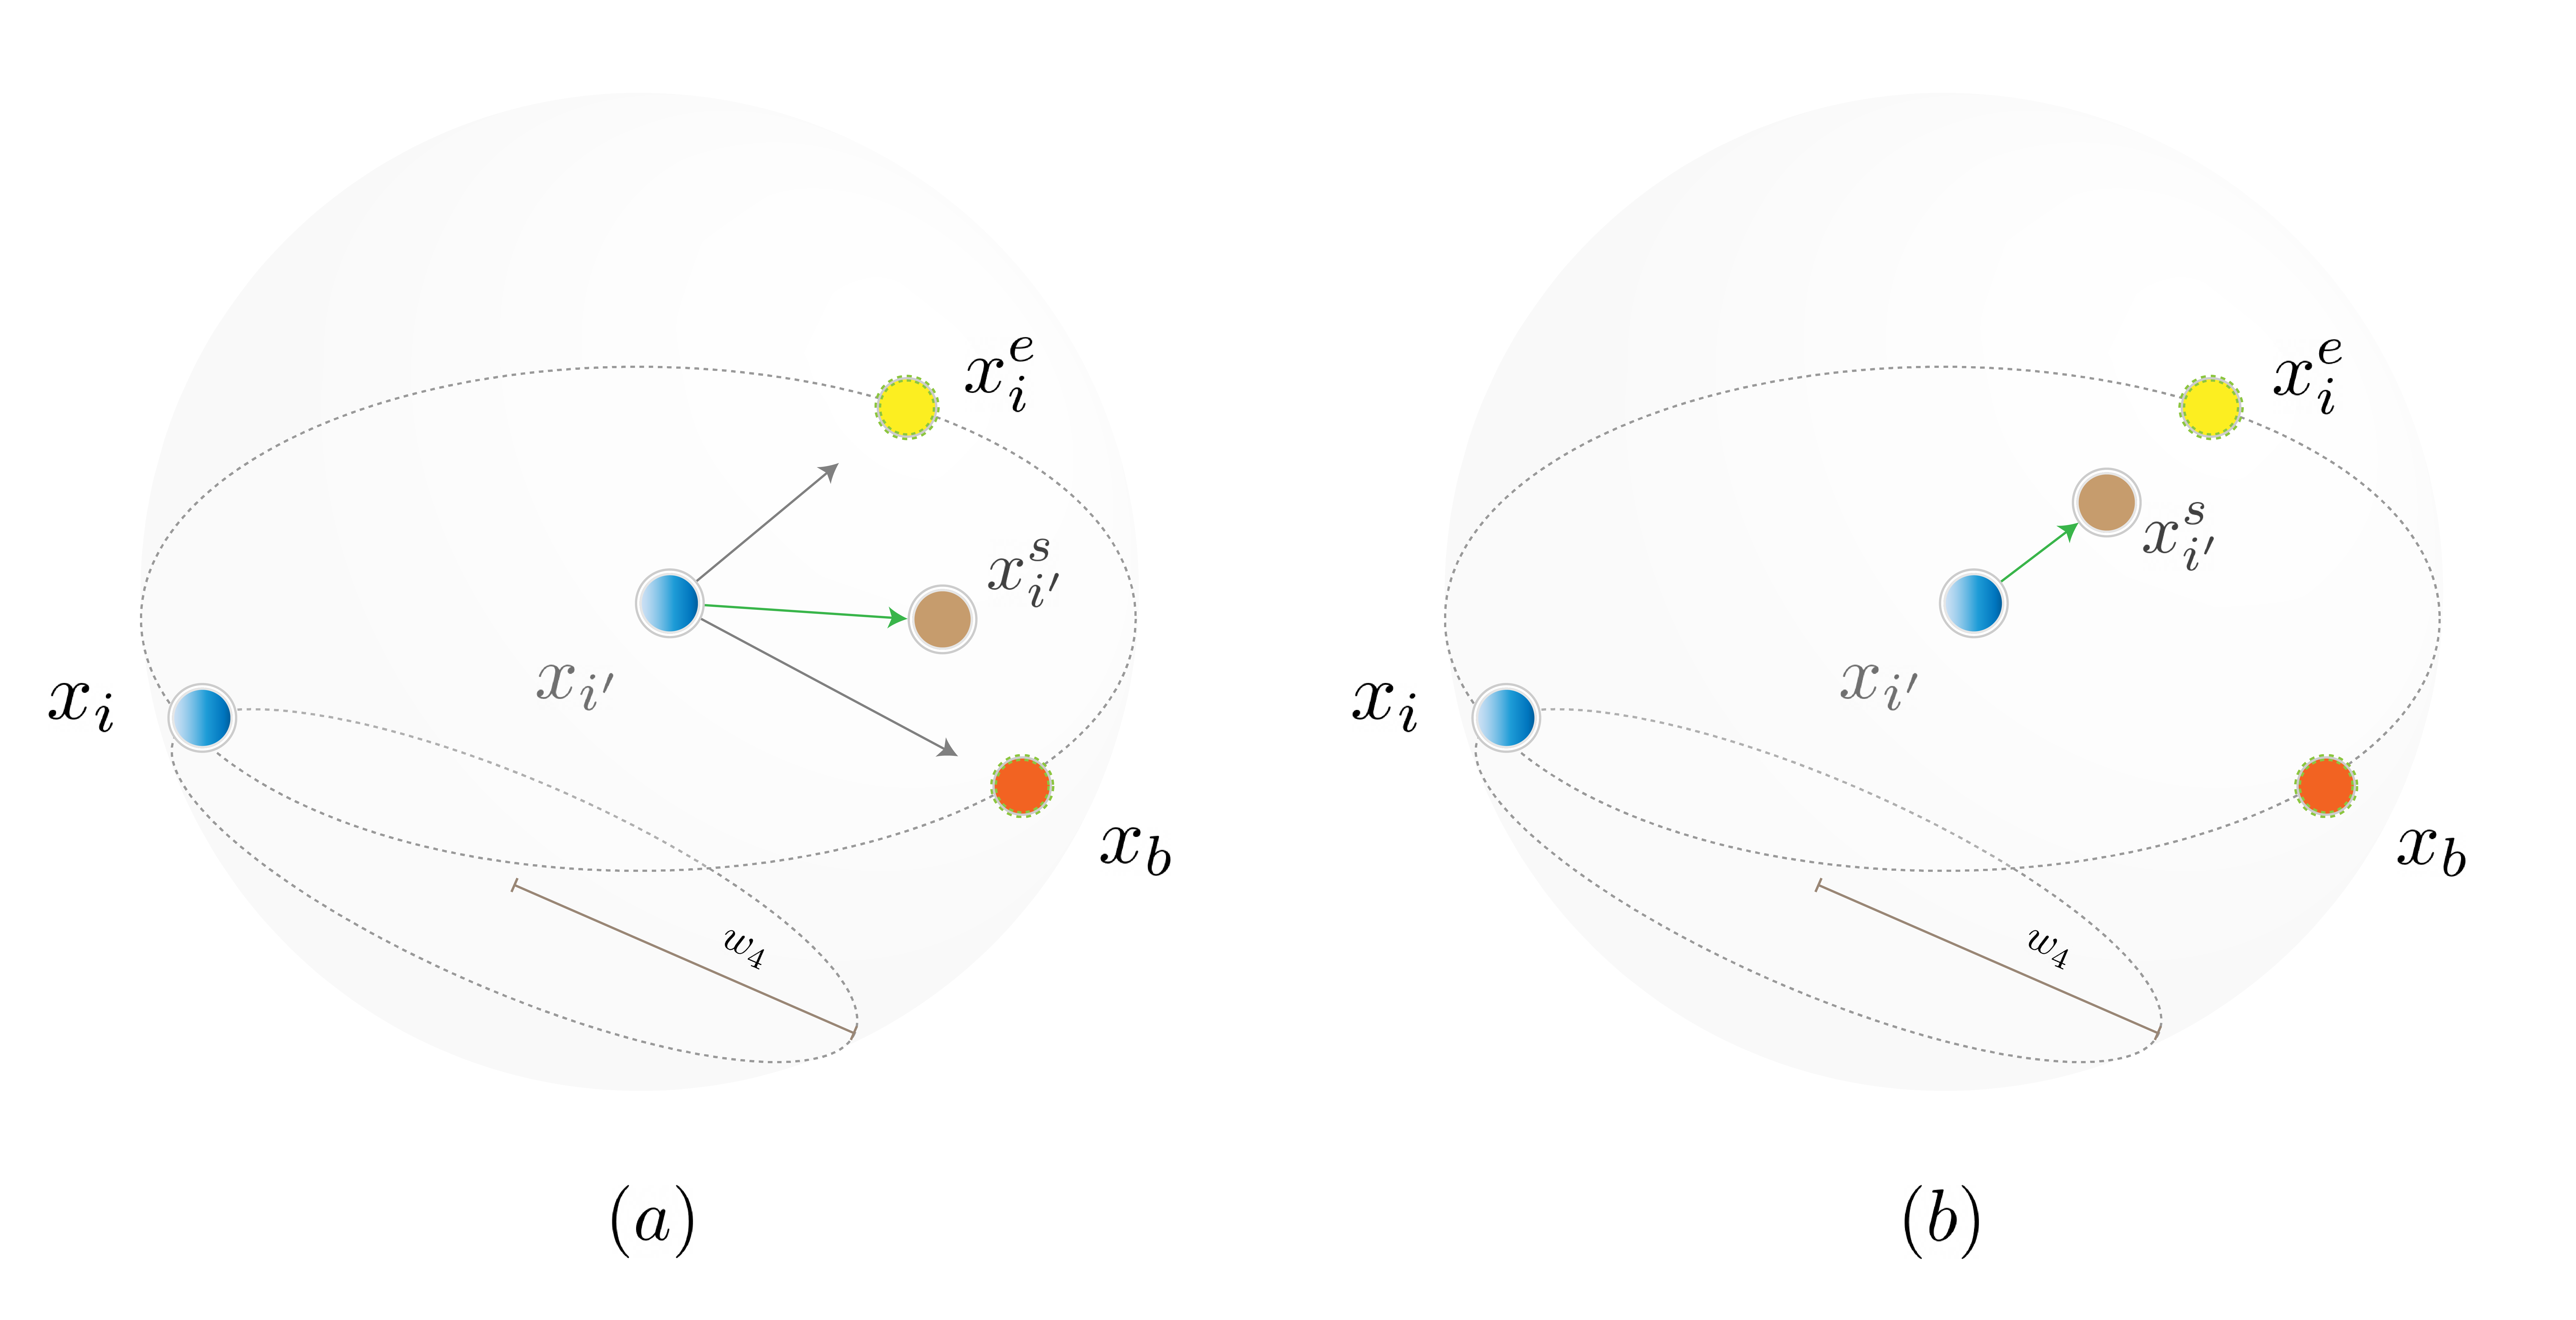
\includegraphics[width=\textwidth]{figures/chapter4/fig03_resource_acquisition.png}
  \bicaption{SBO的资源获取阶段}{Resource Acquisition phase of SBO.}
  \label{fig:resource_acquisition}
\end{figure}


\subsubsection{3.2.4 资源评估}

在资源评估阶段，算法评估获取的资源是否增强了个体的适应度。使用之前建立的标志向量，跟踪进展情况：

\begin{enumerate}
\item  1 = 适应度改善（成功）

\item  0 = 无改善（失败）
\end{enumerate}



实际上，如果更新后个体$x^s_i$的目标函数值优于原始$x_i$，则保留新状态：

\begin{equation}
\label{sbo_eq_10}
\begin{array}{cc}
x_i=x^s_i & if\ fobj\left(x^s_i\right)<fobj\left(x_i\right) \end{array}
\end{equation}

同时，标志向量按如下方式更新：

\begin{equation}
\label{sbo_eq_11}
flag_i=\left\{ \begin{array}{cc}
1 & if\ fobj\left(x^s_i\right)<fobj\left(x_i\right) \\ 
0 & Otherwise \end{array}
\right.
\end{equation}

未表现出改善的个体保持其当前位置，而成功的个体则迁移到更优位置。这种选择性过程反映了现实世界的社会进步，其中只有有价值的资源——那些明显改善代理地位的资源——才被保留。这种精炼过程逐步将搜索引向最优解。

\noindent 
\subsubsection{3.2.5 巩固}

巩固阶段在满足终止条件时激活，即达到最大函数评估次数或获得足够优化的解（通过改进指标验证）。在此之前，算法反复循环其核心阶段：

\begin{enumerate}
\item  \textbf{精英接触}

\item \textbf{资源获取}

\item \textbf{资源评估}
\end{enumerate}



每个阶段模拟地位驱动的交互以逐步改进解。

\textbf{实现细节}：

\begin{enumerate}
\item  \textbf{算法1}提供伪代码

\item  \textbf{图4}展示工作流程
\end{enumerate}

\noindent \textbf{}

在巩固阶段，算法：

\begin{enumerate}
\item  根据目标\textbf{汇编和评估}结果

\item  \textbf{产生}体现基于地位启发式的最终解

\item  \textbf{确保}资源的高效利用和用于分析/应用的详细文档
\end{enumerate}



\begin{tabular}{|p{3.9in}|} \hline 
\textbf{Algorithm }1 Pseudo-code for the Status-based Optimization \\ \hline 
Input $N,\ D,\ MaxFEs,\ lb,\ ub,\ fobj$;\textit{} \\ \hline 
Initialization: \\ \hline 
    Initialize \textit{X}$,\ {\ X}^e,\ Fit,\ Fit^e,\ flag$; \\ \hline 
    Calculate $Fit$ and $Fit^e$; \\ \hline 
    Update $X^e$ and $x_b$; \\ \hline 
\textbf{While} $FEs\ <\ MaxFEs$ \\ \hline 
    Select $x^e_r$ from $X^e$ by Rolette Wheel; \\ \hline 
    Elite Engagement: \\ \hline 
        Update $w_1,\ w_2,\ w_3,\ and\ w_4$; \\ \hline 
        Update $X$ by Eq.~\eqref{sbo_eq_4}; \\ \hline 
        Apply Boundary control to $X$; \\ \hline 
        Initialize $X^s$ as $X$; \\ \hline 
    Resource Acquisition: \\ \hline 
        Initialize row vector $m$ as 0; \\ \hline 
        Update $m$ by Eq.~\eqref{sbo_eq_9};\newline         \textbf{For} each $x^s$ in $X^s$:\newline             \textbf{If} $x^s$ is successful: \\ \hline 
                Update $x^s$ by Eq.~\eqref{sbo_eq_7}; \\ \hline 
            \textbf{Else}:\textbf{} \\ \hline 
                Update $x^s$ by Eq.~\eqref{sbo_eq_8};\newline        \textbf{ End For} \\ \hline 
    Resource Evaluation:\textbf{} \\ \hline 
        Update $X$ by Eq.~\eqref{sbo_eq_10}; \\ \hline 
        Update $flag$ by Eq.~\eqref{sbo_eq_11}; \\ \hline 
    Consolidation: \\ \hline 
\textbf{        }Update $X^e$ and $x_b$;\textit{} \\ \hline 
\textbf{        }Increment\textbf{ }$FEs=FEs+2N$; \\ \hline 
\textbf{End While} \\ \hline 
\textbf{Return} $x_b$. \\ \hline 
\end{tabular}



\begin{figure}[htbp]
  \centering
  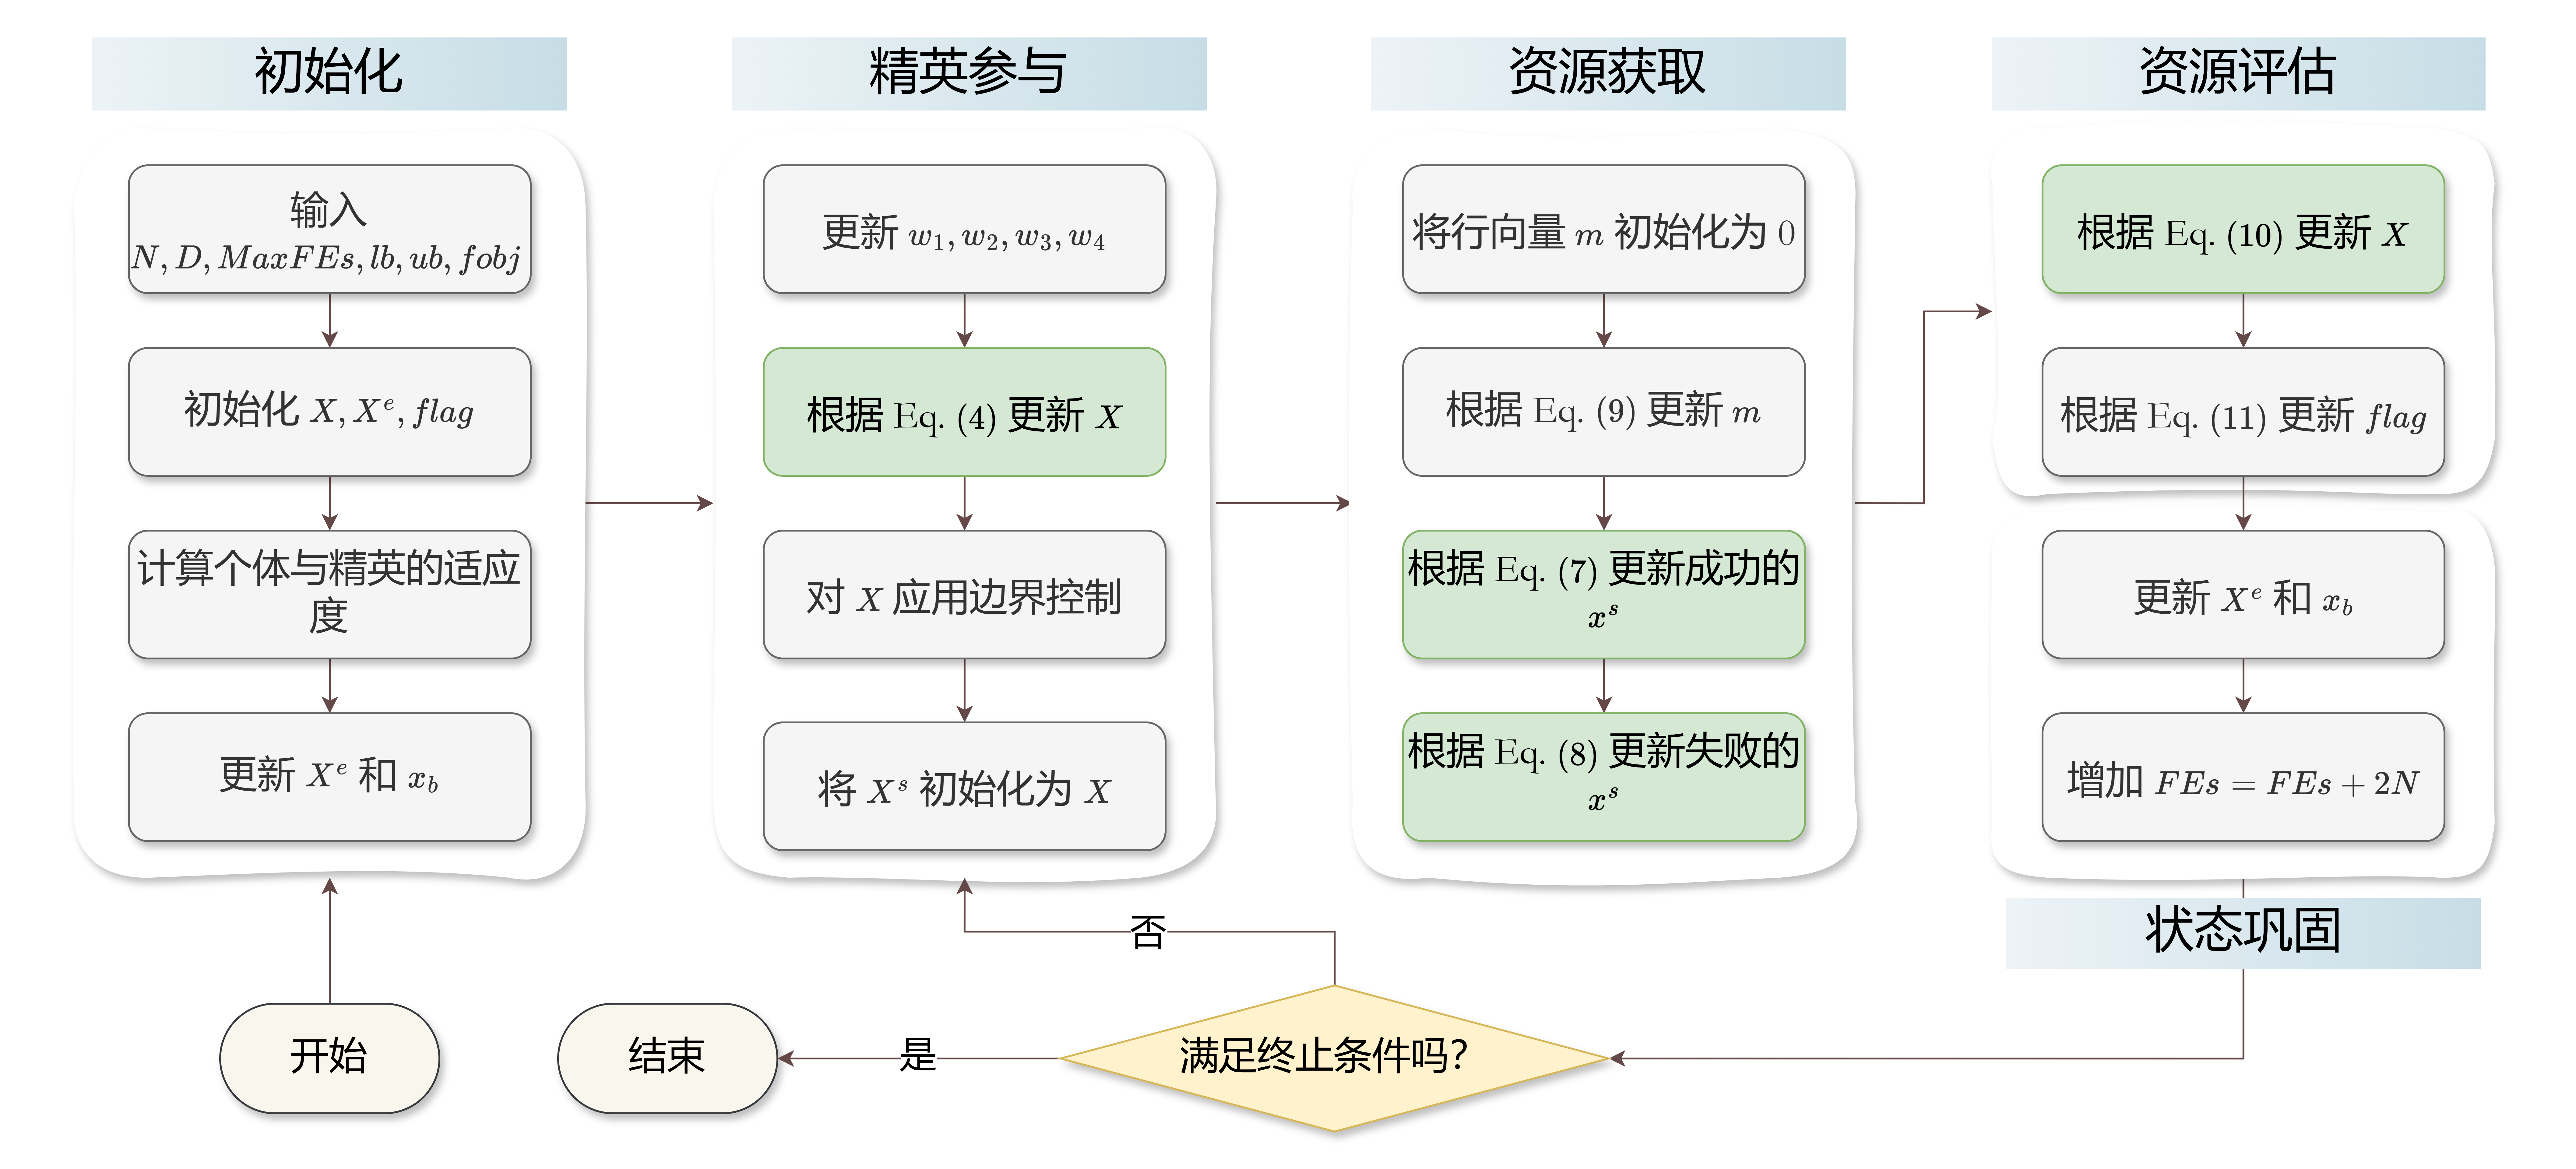
\includegraphics[width=\textwidth]{figures/chapter4/fig04_flowchart_SBO.png}
  \bicaption{SBO算法流程图}{Flowchart of SBO.}
  \label{fig:flowchart_SBO}
\end{figure}




\subsection{SBO的计算复杂度分析}

SBO算法的计算复杂度主要由种群大小（$N$）、问题维度（$D$）和最大迭代次数（$T$）决定，它们共同定义了终止条件。在本分析中，本文关注算法中计算量最大的操作，同时忽略影响较小的向量更新。初始化阶段涉及生成两个大小为$N\times D$的种群，需要$O(2ND)$的时间。精英接触阶段在每次迭代中以$O(ND)$的时间更新解，在$T$次迭代中总计复杂度为$O(TND)$。资源获取和资源评估阶段在每次迭代中均以$O(N)$的时间运行，累计贡献$O(TN)$，而涉及排序的巩固阶段增加了$O(TNlogN)$的整体成本。汇总这些贡献，SBO的总计算复杂度表示为$O(TND+TN+TNlogN)$，该公式概括了其核心操作的顺序和相互依赖特性。该分析为算法在解决各种优化挑战时的效率和可扩展性提供了简洁的定量估计。


\section{SBO的性能评估}

以下各节通过涉及13种最先进算法和IEEE CEC 2017\cite{sbo_ref48}所定义的29个函数的基准测试比较，对所提SBO算法进行了深入的质量评估。这些基准函数因其多样性和全面性而被精心选择——它们包括单峰、多峰、混合和组合函数，共同涵盖了现实世界问题中遇到的广泛优化挑战。这套严格的基准测试套件在优化社区中被广泛认可和使用，为评估SBO的独特特性提供了稳健的框架，例如其搜索动态中的平衡性和多样性，以及通过详细检查观察到的代理轨迹模式。

本次比较的性能指标基于每个函数30次独立运行，平均适应度值（Avg）和标准差（Std）作为算法能力的主要指标。所有实验均在受控环境中进行，以确保公平性和可重复性。

具体而言，所有算法均在配备Intel{\circledR} Xeon{\circledR} Silver 4210R CPU和128 GB RAM的Windows Server 2016平台上进行评估，种群大小为30，每次运行最大目标评估次数为300,000。MATLAB R2018a生态系统为这项广泛的比较研究提供了可靠且标准化的计算基础。


\subsection{SBO的质量分析}

本节评估SBO平衡探索与开发的能力——这是有效元启发式算法的关键方面。本文评估其从广泛的全局搜索转向聚焦的局部精炼的能力，同时管理种群多样性，这通过其搜索代理的历史分布和轨迹来揭示。该分析突出了多样化和收敛之间的相互作用，为SBO在导航复杂解空间中的效率提供了见解。

为量化这种平衡，本文使用测量探索（搜索新区域，增加多样性）和开发（精炼已知良好解，减少多样性）的指标。一个实用的算法通常表现为早期强探索，随后加强开发。本文采用逐维度多样性度量\cite{sbo_ref49}：

\begin{equation}
\label{sbo_eq_12}
Div=\frac{1}{D}\int^D_{j=1}{Div_j}
\end{equation}

\begin{equation}
\label{sbo_eq_13}
Div_j=\frac{1}{N}\int^N_{i=1}{\left|X^j_i-mean\left(X^j\right)\right|}
\end{equation}

\begin{equation}
\label{sbo_eq_14}
mean\left(X^j\right)=\frac{1}{N}\int^N_{i=1}{X^j_i}
\end{equation}

其中$Div_j$是第$jth$维度的多样性，$D$是问题维度，$X^j_i$是第$ith$个解的第$jth$坐标。基于此，本文定义探索率和开发率如下：

\begin{equation}
\label{sbo_eq_15}
Exploration=\frac{Div\left(t\right)}{Div_{max}}\times 100\%
\end{equation}

\begin{equation}
\label{sbo_eq_16}
Exploitation=\frac{\left|Div\left(t\right)-Div_{max}\right|}{Div_{max}}\times 100\%
\end{equation}

其中$Div(t)$是迭代$t$时的多样性，$Div_{max}$是观察到的最大多样性。

在实验中，本文设置种群大小$N=30$，问题维度$D=30$，最多允许300,000次评估。图5展示了IEEE CEC 2017套件中八个函数的探索率、开发率、种群多样性和收敛曲线。

选择用于分析的函数涵盖了IEEE CEC 2017套件的所有四个类别。具体而言，本文考虑了单峰函数F1，多峰函数F3和F9，混合函数F11、F13、F16和F19，以及组合函数F26。它们的三维分布如图5(a)所示。单峰函数具有单一全局最优，主要测试算法的收敛和探索效率。相比之下，多峰函数评估逃离局部最优的能力，而混合和组合函数通过组合、旋转和移位形成，挑战算法有效平衡探索和开发。

图5(b)表明SBO在早期迭代中表现出高探索率，在后期阶段转为以开发为主。平衡曲线中的递增-递减趋势反映了这种转变：初始上升表示强劲的全局探索，而随后的下降指向聚焦的局部开发。例如，对于F1，开发率达到93.9\%，突显了SBO在向最优解精炼方面的能力。

此外，图5(b)和图5(c)揭示SBO的种群多样性在稳定之前稳步下降，表明解的质量持续改善。多峰函数F3和F9表现出与F1类似的模式，但由于其复杂性，探索率略高。在混合函数的情况下，探索率的显著增加（F13最高达到23.3\%）加上多样性的明显波动，导致收敛速度比单峰和多峰情况慢。然而，图5(d)中的收敛曲线确认SBO通过逐步精炼解有效避免了局部最优。对于组合函数F26，12.7\%的探索率和多样性的逐渐下降突显了SBO在全局探索和局部开发之间的灵巧平衡，其特征是初始探索活动的激增，随后进入聚焦精炼阶段。

\begin{figure}[htbp]
  \centering
  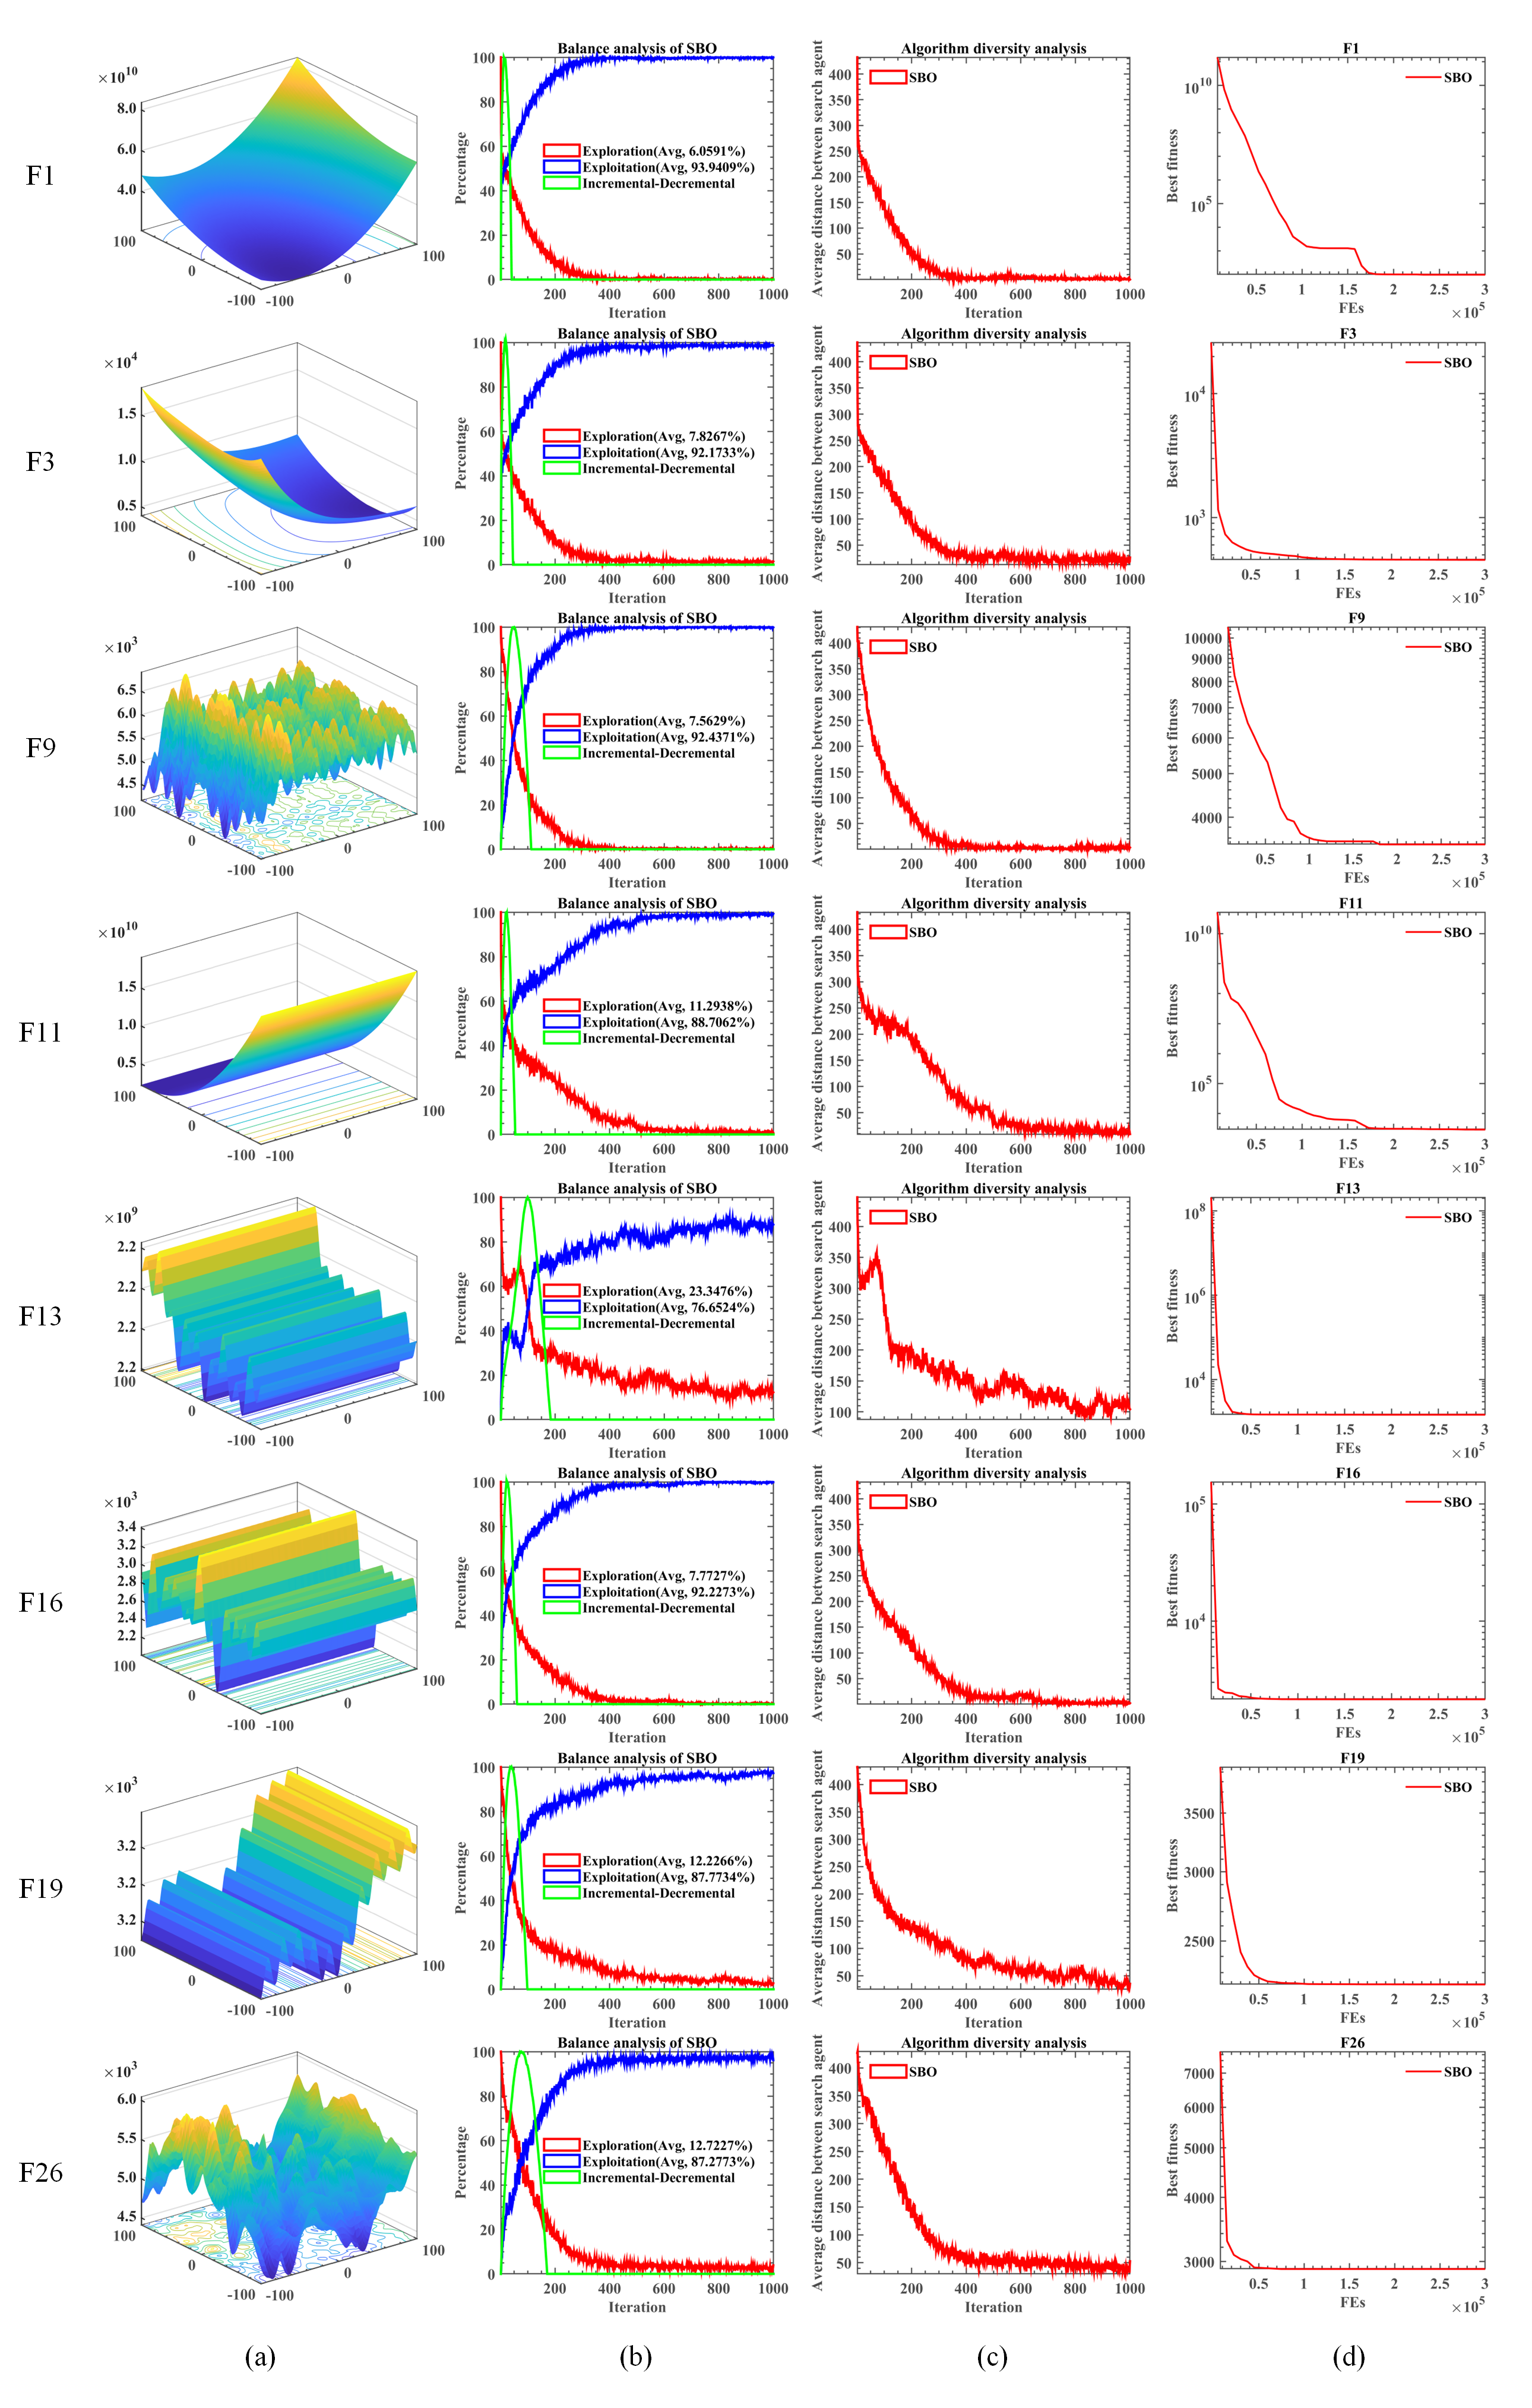
\includegraphics[width=\textwidth]{figures/chapter4/fig05_balance_diversity_convergence.png}
  \bicaption{(a) 函数三维图, (b) SBO平衡分析, (c) SBO多样性分析, (d) SBO收敛曲线}{(a) 3D plots of functions, (b) balance analysis of SBO, (c) diversity analysis of SBO, (d) convergence curves of SBO.}
  \label{fig:balance_diversity_convergence}
\end{figure}



为了研究SBO算法，本文在200次迭代中采用了四种评估指标，种群大小恒定为30。这些指标能够对算法的行为和有效性进行全面的定性评估。特别是，从第一次到最后一次迭代记录了代理的搜索历史，提供了算法在整个搜索空间中探索和开发运动的见解。此外，分析了最佳搜索代理的轨迹，由连续代际中第一维变量的变化来表示，以说明从初始探索到后续开发的进展。在整个进化过程中计算了搜索代理的平均适应度，以捕获算法的整体改进。相比之下，由种群随时间获得的最佳适应度值定义的收敛曲线，提供了通向最优解的精炼过程的可视化表示。

这些指标应用于从23个经典基准函数集中选择的八个函数，其三维表示如图6(a)所示。图6(b)展示了SBO算法代理的搜索历史，其中最优解由红点标记，各个代理由黑点标记。代理在整个搜索空间中的广泛分散，加上在最优值附近的明显聚集，突显了算法强大的探索能力及其有效的局部开发。这种行为的双重性归因于SBO中固有的不同战略阶段，其中探索主要在精英接触阶段得到加强，而开发则通过最有前景个体之间的资源分配来提升。

图6(c)提供了进一步分析，绘制了最佳搜索代理第一维变量的轨迹。初始迭代表现出显著的波动，最终趋于稳定，反映了算法从强力探索阶段到聚焦开发阶段的转变。类似地，图6(d)说明代理的平均适应度从较高水平开始，随着过程的推进而稳定或在窄范围内波动，表明逐渐向最优收敛。

\begin{figure}[htbp]
  \centering
  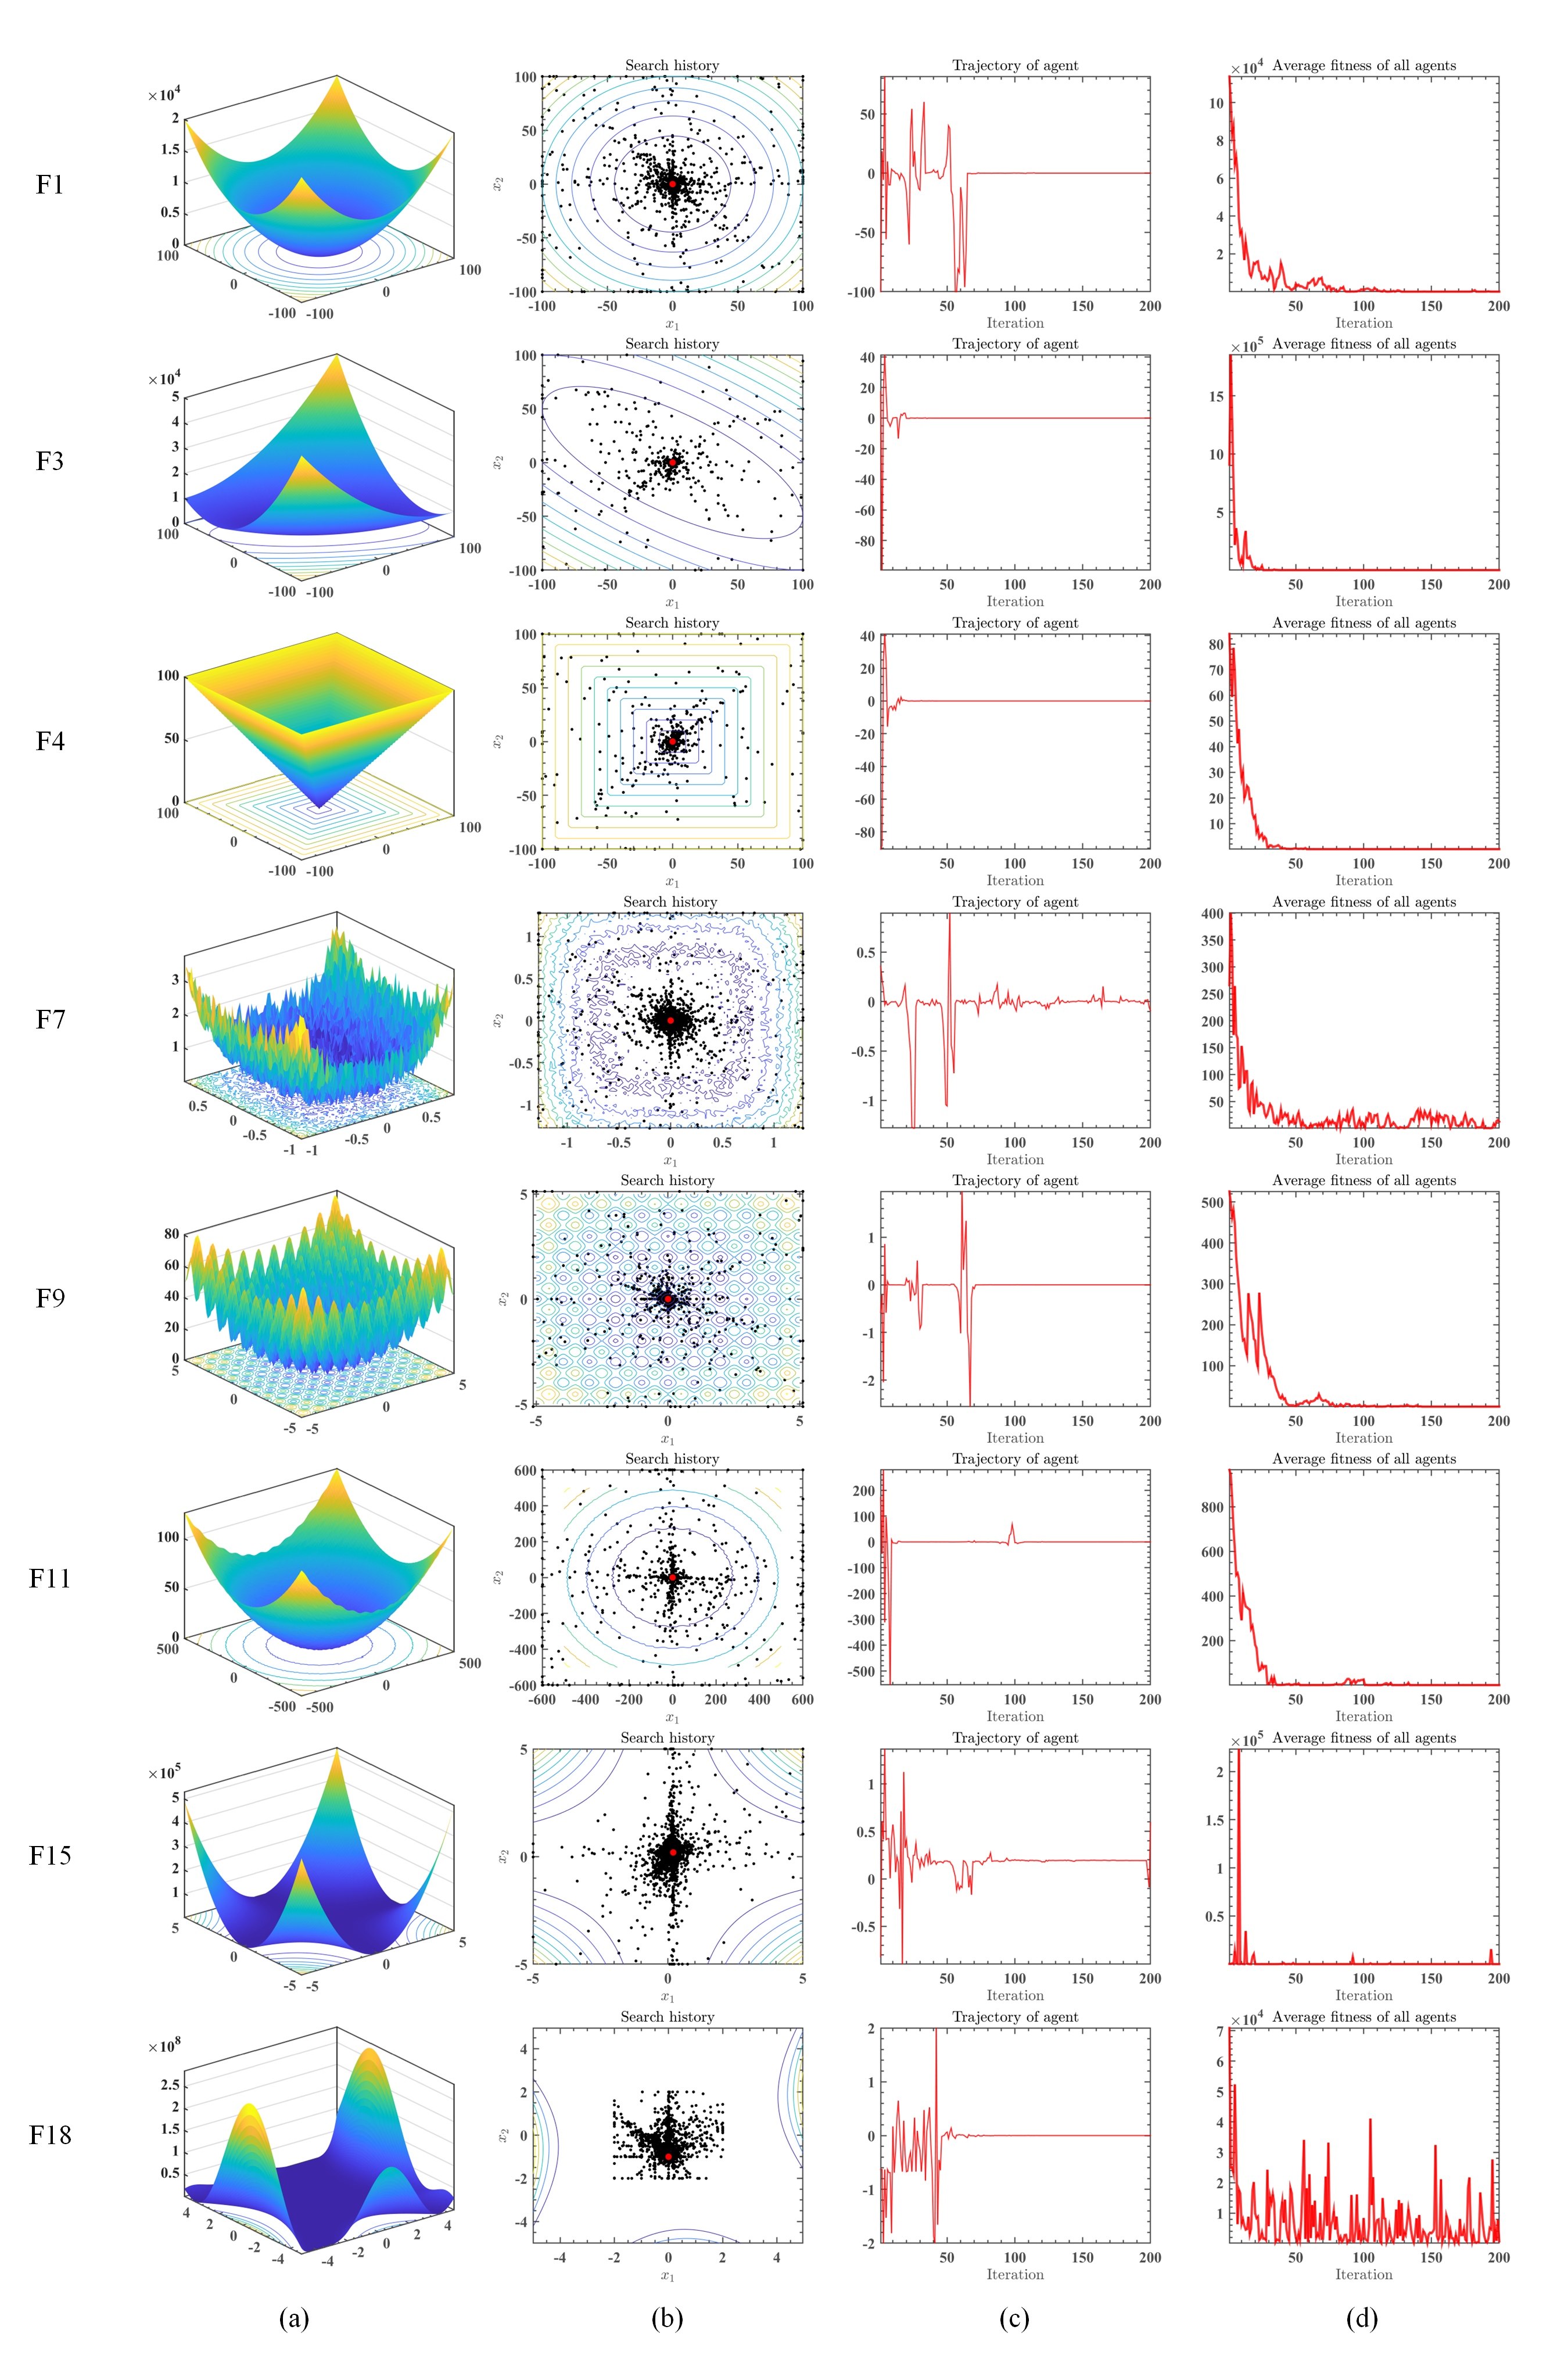
\includegraphics[width=\textwidth]{figures/chapter4/fig06_search_history_trajectory.png}
  \bicaption{(a) 函数三维图, (b) 搜索历史, (c) 代理轨迹, (d) 所有代理的平均适应度}{(a) 3D plots of functions (b) search history, (c) trajectory of agent, (d) average fitness of all agents.}
  \label{fig:search_history_trajectory}
\end{figure}



对SBO算法的综合性能分析提供了对其功能的重要见解，特别关注候选解在整个优化过程中如何演化和改进。该分析展示了SBO独特战略阶段——精英接触和资源获取——的有效性，这些阶段基于人类寻求地位的行为。通过复制人类追求社会向上流动的行为，算法驱动了对搜索空间的广泛探索，反映了通过与成功个体建立联系来进步的自然驱动力。同时，精英代理之间信息和资源的战略交换实现了聚焦开发，改进了候选解。这种植根于地位驱动社会动态的探索与开发的有效整合，赋予了SBO解决复杂优化挑战的强大能力。


\subsection{SBO的基准测试比较}

使用IEEE CEC 2017基准测试套件的29个函数对所提SBO算法的性能进行了全面评估，测试覆盖了10、30、50和100的维度以检验可扩展性。

\textbf{函数类别包括}：

\begin{enumerate}
\item  \textbf{单峰（F1-F2）}：测试开发和收敛能力

\item  \textbf{多峰（F3-F9）}：评估避免局部最优和探索能力

\item  \textbf{混合（F10-F19）}和\textbf{组合（F20-F29）}：评估探索/开发之间的平衡
\end{enumerate}

这些精心选择的函数（详见表1）创建了一个严格的测试环境，用于分析SBO的性能特征。



\noindent \textbf{}

\begin{tabular}{|p{0.3in}|p{1.5in}|p{0.5in}|p{0.5in}|p{0.5in}|p{0.5in}|} \hline 
\multicolumn{6}{|p{1in}|}{\textbf{Table }1\textbf{.} Information of IEEE CEC 2017.\textbf{}} \\ \hline 
ID & Description & Type & Dimension & Range & Optimum \\ \hline 
F1 & Shifted and Rotated Bent Cigar Function & Unimodal & 10,30,50,100 & [-100,100] & 100 \\ \hline 
F2 & Shifted and Rotated Zakharov function & Unimodal & 10,30,50,100 & [-100,100] & 300 \\ \hline 
F3 & Shifted and Rotated Rosenbrock's function & Multimodal & 10,30,50,100 & [-100,100] & 400 \\ \hline 
F4 & Shifted and Rotated Rastrigin's function & Multimodal & 10,30,50,100 & [-100,100] & 500 \\ \hline 
F5 & Shifted and Rotated Expanded Scaffer's function & Multimodal & 10,30,50,100 & [-100,100] & 600 \\ \hline 
F6 & Shifted and Rotated Lunacek Bi-Rastrigin function & Multimodal & 10,30,50,100 & [-100,100] & 700 \\ \hline 
F7 & Shifted and Rotated Non-Continuous Rastrigin's function & Multimodal & 10,30,50,100 & [-100,100] & 800 \\ \hline 
F8 & Shifted and Rotated L\'{e}vy function & Multimodal & 10,30,50,100 & [-100,100] & 900 \\ \hline 
F9 & Shifted and Rotated Schwefel's function & Multimodal & 10,30,50,100 & [-100,100] & 1000 \\ \hline 
F10 & Hybrid Function 1 (N=3) & Hybrid & 10,30,50,100 & [-100,100] & 1100 \\ \hline 
F11 & Hybrid Function 2 (N=3) & Hybrid & 10,30,50,100 & [-100,100] & 1200 \\ \hline 
F12 & Hybrid Function 3 (N=3) & Hybrid & 10,30,50,100 & [-100,100] & 1300 \\ \hline 
F13 & Hybrid Function 4 (N=4) & Hybrid & 10,30,50,100 & [-100,100] & 1400 \\ \hline 
F14 & Hybrid Function 5 (N=4) & Hybrid & 10,30,50,100 & [-100,100] & 1500 \\ \hline 
F15 & Hybrid Function 6 (N=4) & Hybrid & 10,30,50,100 & [-100,100] & 1600 \\ \hline 
F16 & Hybrid Function 6 (N=5) & Hybrid & 10,30,50,100 & [-100,100] & 1700 \\ \hline 
F17 & Hybrid Function 6 (N=5) & Hybrid & 10,30,50,100 & [-100,100] & 1800 \\ \hline 
F18 & Hybrid Function 6 (N=5) & Hybrid & 10,30,50,100 & [-100,100] & 1900 \\ \hline 
F19 & Hybrid Function 6 (N=6) & Hybrid & 10,30,50,100 & [-100,100] & 2000 \\ \hline 
F20 & Composition Function 1 (N=3) & Composition & 10,30,50,100 & [-100,100] & 2100 \\ \hline 
F21 & Composition Function 2 (N=3) & Composition & 10,30,50,100 & [-100,100] & 2200 \\ \hline 
F22 & Composition Function 3 (N=4) & Composition & 10,30,50,100 & [-100,100] & 2300 \\ \hline 
F23 & Composition Function 4 (N=4) & Composition & 10,30,50,100 & [-100,100] & 2400 \\ \hline 
F24 & Composition Function 5 (N=5) & Composition & 10,30,50,100 & [-100,100] & 2500 \\ \hline 
F25 & Composition Function 6 (N=5) & Composition & 10,30,50,100 & [-100,100] & 2600 \\ \hline 
F26 & Composition Function 7 (N=6) & Composition & 10,30,50,100 & [-100,100] & 2700 \\ \hline 
F27 & Composition Function 8 (N=6) & Composition & 10,30,50,100 & [-100,100] & 2800 \\ \hline 
F28 & Composition Function 9 (N=3) & Composition & 10,30,50,100 & [-100,100] & 2900 \\ \hline 
F29 & Composition Function 10 (N=3) & Composition & 10,30,50,100 & [-100,100] & 3000 \\ \hline 
\end{tabular}



为了验证SBO，本文与13种最先进的算法进行了比较分析，这些算法基于其多样性、相关性和在先前研究中的性能优势而被选择。这些算法代表了多种优化策略，包括人类行为启发方法、群体智能和进化技术。选择包括两种人类行为启发算法，即著名的TLBO\cite{sbo_ref30}和广泛认可的PO\cite{sbo_ref37}，以及两种最近提出的具有大量引用的算法：Harris Hawks优化（HHO）\cite{sbo_ref48}和物理启发优化算法RIME\cite{sbo_ref49}。此外，比较还包括四种著名且强大的PSO变体：带老化领导者和挑战者的PSO（ALCPSO）\cite{sbo_ref50}、综合学习粒子群优化（CLPSO）\cite{sbo_ref51}、协作协同进化粒子群优化（CGPSO）\cite{sbo_ref52}和多群粒子群优化（MSPSO）\cite{sbo_ref53}。作为补充的五种进化算法以其冠军地位而著称：协方差矩阵自适应进化策略（CMAES）\cite{sbo_ref54}、带混沌局部搜索的差分进化（DECLS）\cite{sbo_ref55}、集成正弦差分协方差矩阵自适应与欧几里得邻域（LSHADE\_cnEpSin）\cite{sbo_ref56}、正弦余弦算法差分进化（SCADE）\cite{sbo_ref57}和基于成功历史的差分进化参数自适应（SHADE）\cite{sbo_ref58}。表2总结了这些算法的关键特征和参数设置。

为确保客观比较，每种算法的参数设置遵循其原始出版物中推荐的值。这些设置保持了与其预期设计的一致性，并代表了先前研究中确立的最优或近最优配置。所有算法在相同的计算条件下运行：

\begin{enumerate}
\item  固定种群大小：30

\item  最大函数评估次数：300,000

\item  相同的终止条件
\end{enumerate}

这种标准化方法确保了公平的比较，同时避免了由于计算限制而对算法进行特定调整。

分析结果（30次独立运行的Avg和Std）展示了算法在求解基准函数时的稳定性和鲁棒性。虽然本文的方法确保了公平性，但也承认个别参数调整可能进一步提高性能并影响结果。未来的研究将调查这一方面，以实现更完整的基准测试。

此外，由于算法的随机性质，采用了Friedman检验\cite{sbo_ref59}和Wilcoxon符号秩检验\cite{sbo_ref60}等统计评估来分析结果。这些统计检验与平均值和标准差相辅相成，确定了整体性能并对比较结果的统计显著性进行了基准测试。值得注意的是，显著性阈值设为0.05，由此产生的p值表明所提SBO与其竞争对手之间的统计显著性。后续表格将在基准结果之后展示四个不同维度下p值的综合比较。

\noindent 

\begin{tabular}{|p{1.1in}|p{2.8in}|} \hline 
\multicolumn{2}{|p{1in}|}{\textbf{Table }2\textbf{.} Parameter settings for involved algorithms.} \\ \hline 
Algorithm & Other parameters \\ \hline 
TLBO & $None$\textit{} \\ \hline 
PO & $λ=1,n=7$\textit{} \\ \hline 
HHO & $E=\left[-2,2\right]$\textit{} \\ \hline 
RIME & $W=5$\textit{} \\ \hline 
ALCPSO & $w=0.4,c1=2,c2=2,lifespan=60,\ T=2,pro=1/D$\textit{} \\ \hline 
CLPSO & $w_{max}=0.9,w_{min}=0.4,c=1.49445$\textit{} \\ \hline 
CGPSO & $v_{max}=6,c1=2,c2=2$MSPSO \\ \hline 
$v_{max}\mathrm{=6,}v_{\mathrm{min}}\mathrm{=-6,}w_{\mathrm{max}}\mathrm{=0.9,}w_{\mathrm{min}}\mathrm{=0.2,c1=2,c2=2}$CMAES & $λ=4+\left\lfloor 3{ln \left(N\right)\ }\right\rfloor ,w'_i={ln \left(\frac{λ+1}{2}\right)-lni,\ }μ=\left\lfloor \frac{λ}{2}\right\rfloor ,\ {σ=0.3,C}_c=\frac{4}{N+4}$DECLS \\ \hline 
$NP=D,F=0.5,p_{CR}\mathrm{=0.5,L=}\frac{\mathrm{D}}{\mathrm{5}}\mathrm{,m=1500}$LSHADE\_cnEpSin & $NP_{max}=18\times D,NP_{min}=4,H=5,\left|A\right|=1.4\times NP,p=0.11\ $\textit{} \\ \hline 
SCADE & $β_{max}=0.8,β_{min}=0.2,p_{CR}=0.8$\textit{} \\ \hline 
SHADE & $\left|A\right|=2\times NP,p=0.1$ \\ \hline 
 \\ \hline 
 \\ \hline 
\end{tabular}




\subsection{基准测试结果与统计分析}

SBO算法使用IEEE CEC 2017基准测试套件与13种最先进的算法进行了综合评估，该套件包含29个函数，涵盖单峰、多峰、混合和组合类型。这些函数在四个维度（10、30、50和100）上进行测试，以评估SBO的可扩展性、鲁棒性和对不同问题复杂度的适应性。比较结果包括30次独立运行的Avg和Std，详见表A. 1\textbf{--A.4}，对应的p值详见表A. 5\textbf{--A.8}。进行了Friedman检验和Wilcoxon符号秩检验等统计检验以评估结果的显著性，其汇总统计数据见表3。

SBO在所有维度上表现出强劲且一致的性能，在36\%的基准函数中获得平均第一名排名。其优势在混合和组合函数中尤为明显，这些函数中平衡探索和开发至关重要。热力图（图7）可视化了所有算法在各函数和维度上的归一化性能，较暖的颜色表示更优的结果。在此可视化中，SBO频繁脱颖而出，成为表现最优的算法之一，特别是在高维混合和组合函数上，展示了其对复杂优化问题的适应性。



\begin{figure}[htbp]
  \centering
  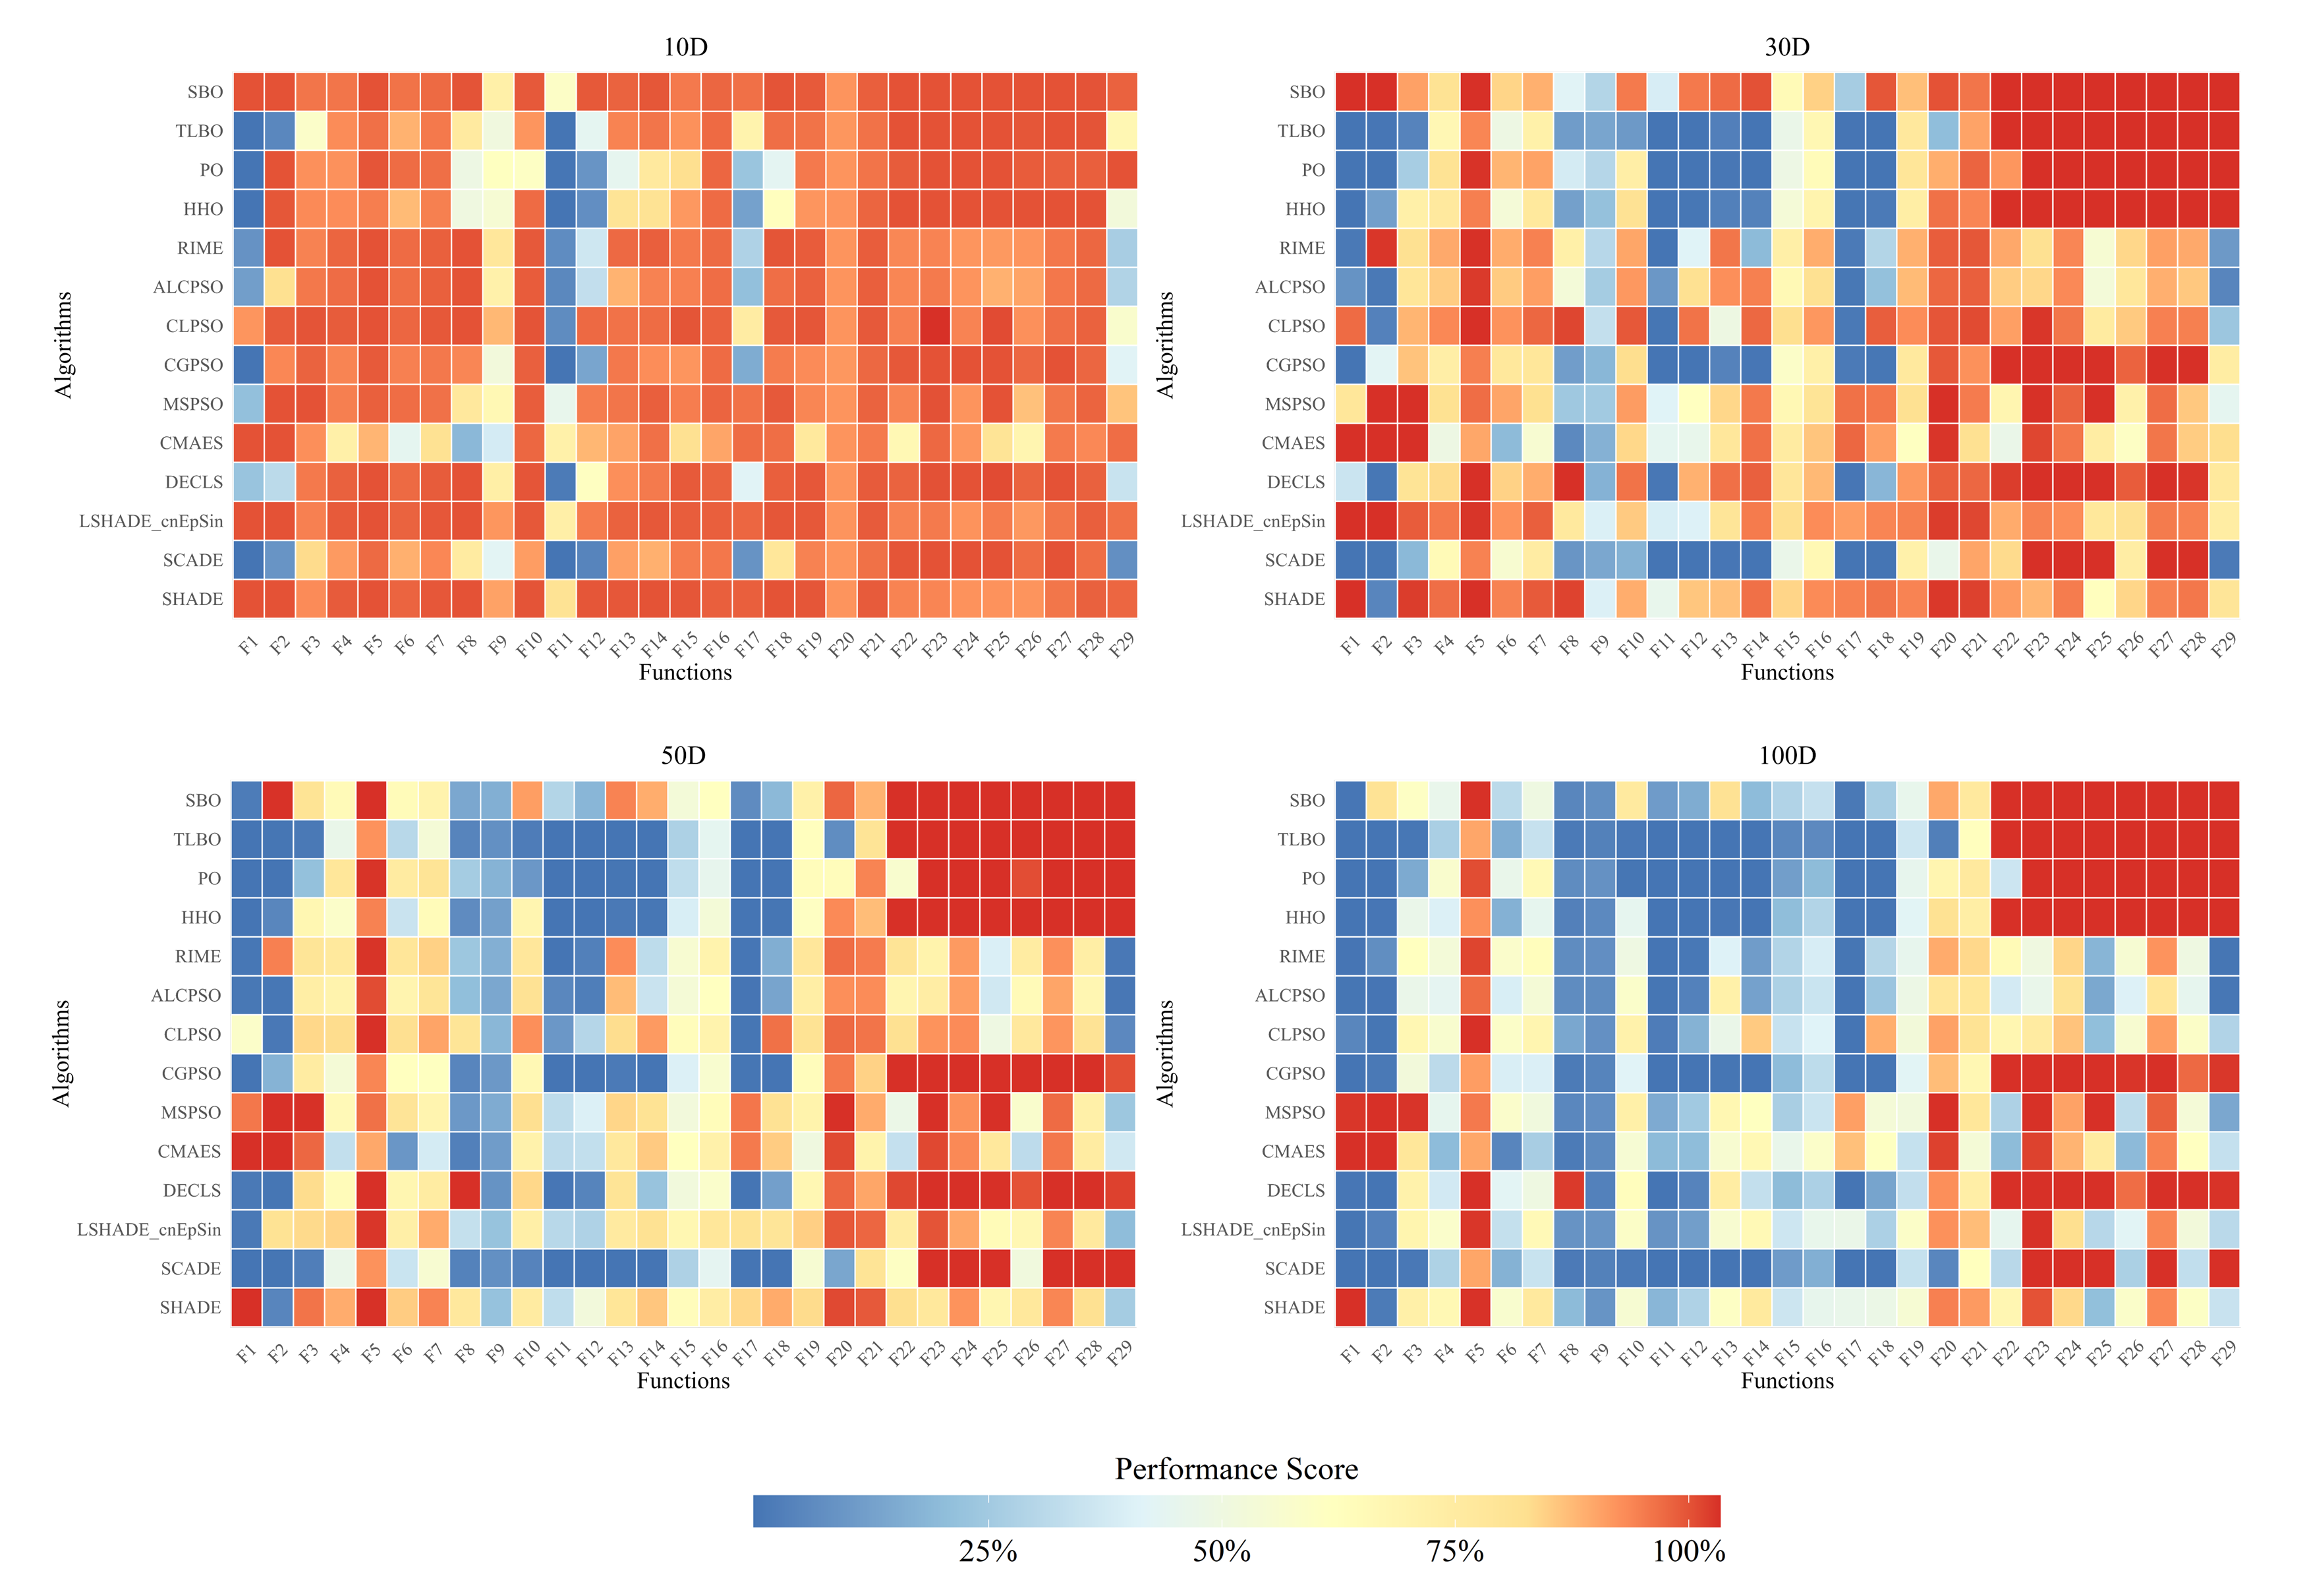
\includegraphics[width=\textwidth]{figures/chapter4/fig07_performance_heatmap.png}
  \bicaption{四个维度下的算法性能热力图}{Algorithm performance heatmap across four dimensions.}
  \label{fig:performance_heatmap}
\end{figure}



在单峰函数（F1--F2）中，这些函数侧重于开发和精度，SBO排名具有竞争力，但略逊于注重精度的算法如CMAES、LSHADE\_cnEpSin和LSHADE。SBO在所有维度上该类别中平均获得第四名，展示了其鲁棒性，尽管在精度上存在轻微的权衡。对于多峰函数（F3--F9），SBO表现出强大的探索能力，持续避免局部最优并获得有竞争力的排名。例如，它在F5中获得第四名，同时在该类别中保持了较高的稳定性。算法的性能在混合（F10--F19）和组合函数（F20--F29）中最为突出，在F13、F14和F22--F29等函数中持续获得第一名。这些结果突显了SBO有效适应需要平衡探索和开发的动态环境的能力。

30维结果为SBO的性能提供了更深入的见解，特别是其收敛行为和鲁棒性。选定基准函数的收敛曲线（图8）说明了SBO在迭代过程中解质量的稳定改善。对于F1和F2等单峰函数，SBO保持了一致的收敛率，在精度上紧随CMAES和LSHADE。在F13、F14和F29等混合和组合函数中，SBO展示了优越的收敛速度，反映了其识别搜索空间中有前景区域同时避免过早停滞的能力。此外，SBO在30次独立运行中性能的箱线图（图9）揭示了其与TLBO和PO等算法相比方差较低，后者表现出较高的变异性。这种稳定性突显了SBO的可靠性，特别是对于一致性能至关重要的混合和组合函数。



\begin{figure}[htbp]
  \centering
  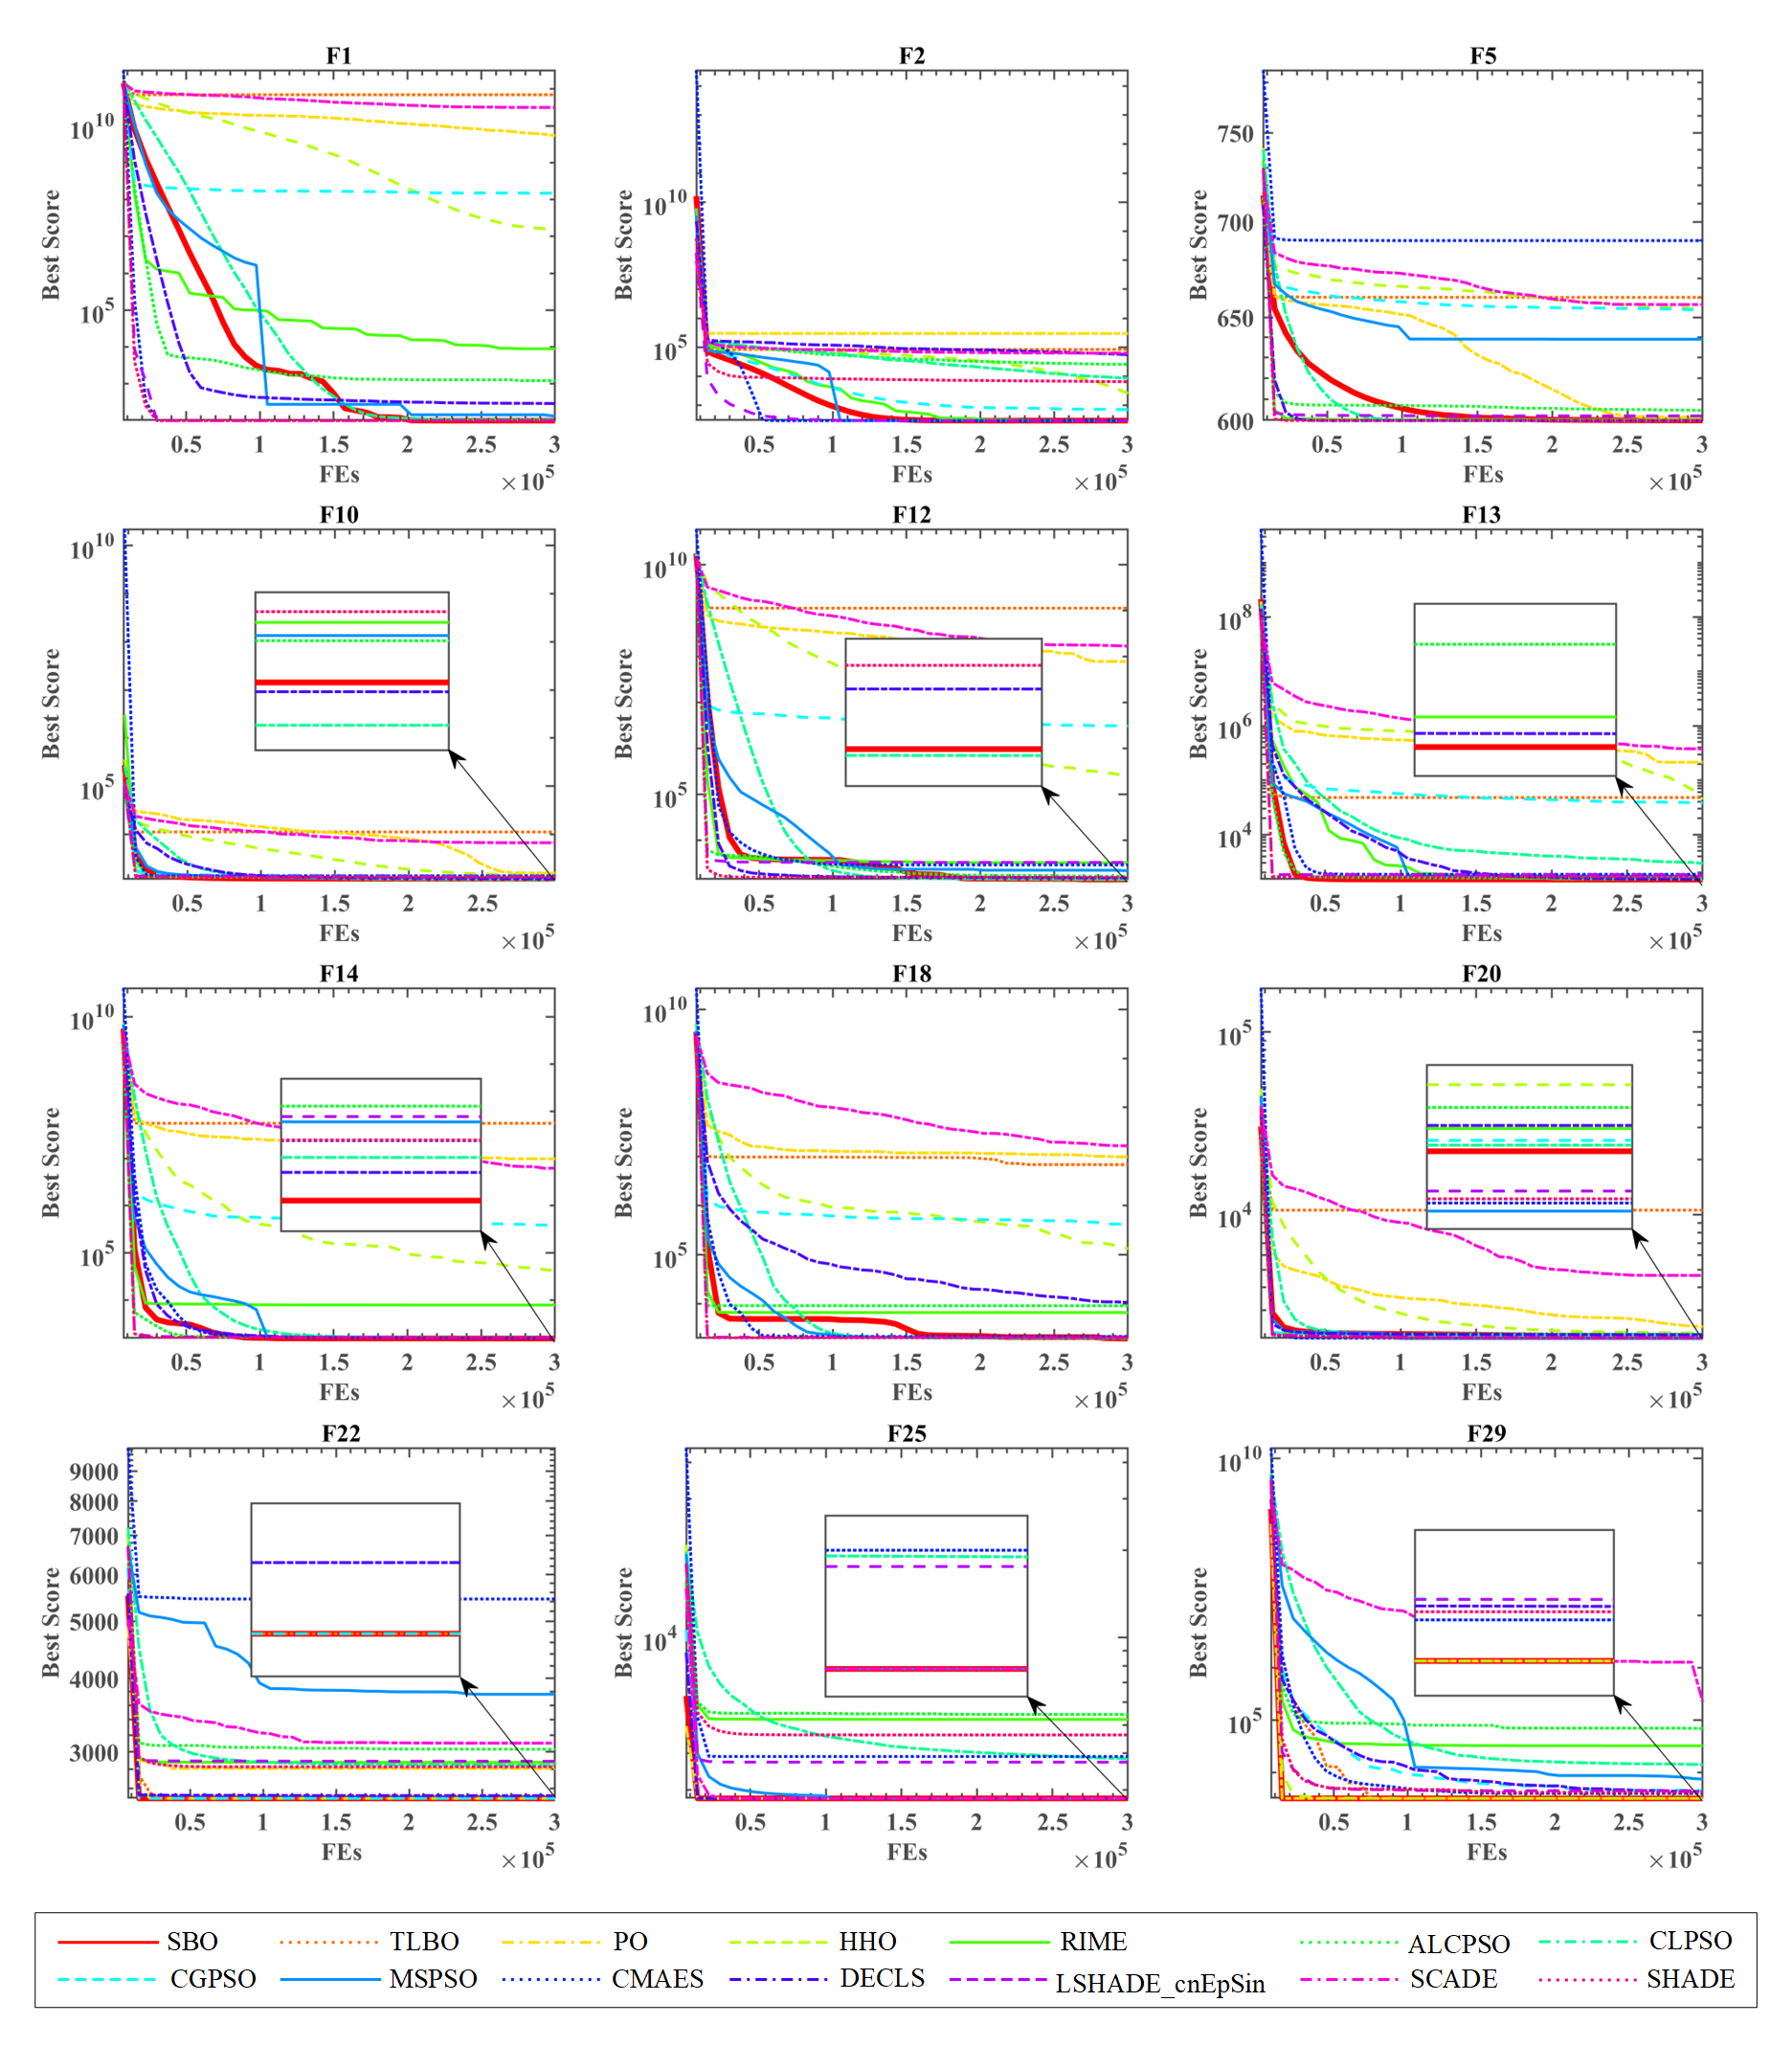
\includegraphics[width=\textwidth]{figures/chapter4/fig08_convergence_curves_30dim.png}
  \bicaption{SBO与先进算法在30维问题上的收敛曲线}{Convergence curves of SBO and state-of-the-art algorithms for 30-dimensional problems.}
  \label{fig:convergence_curves_30dim}
\end{figure}



\begin{figure}[htbp]
  \centering
  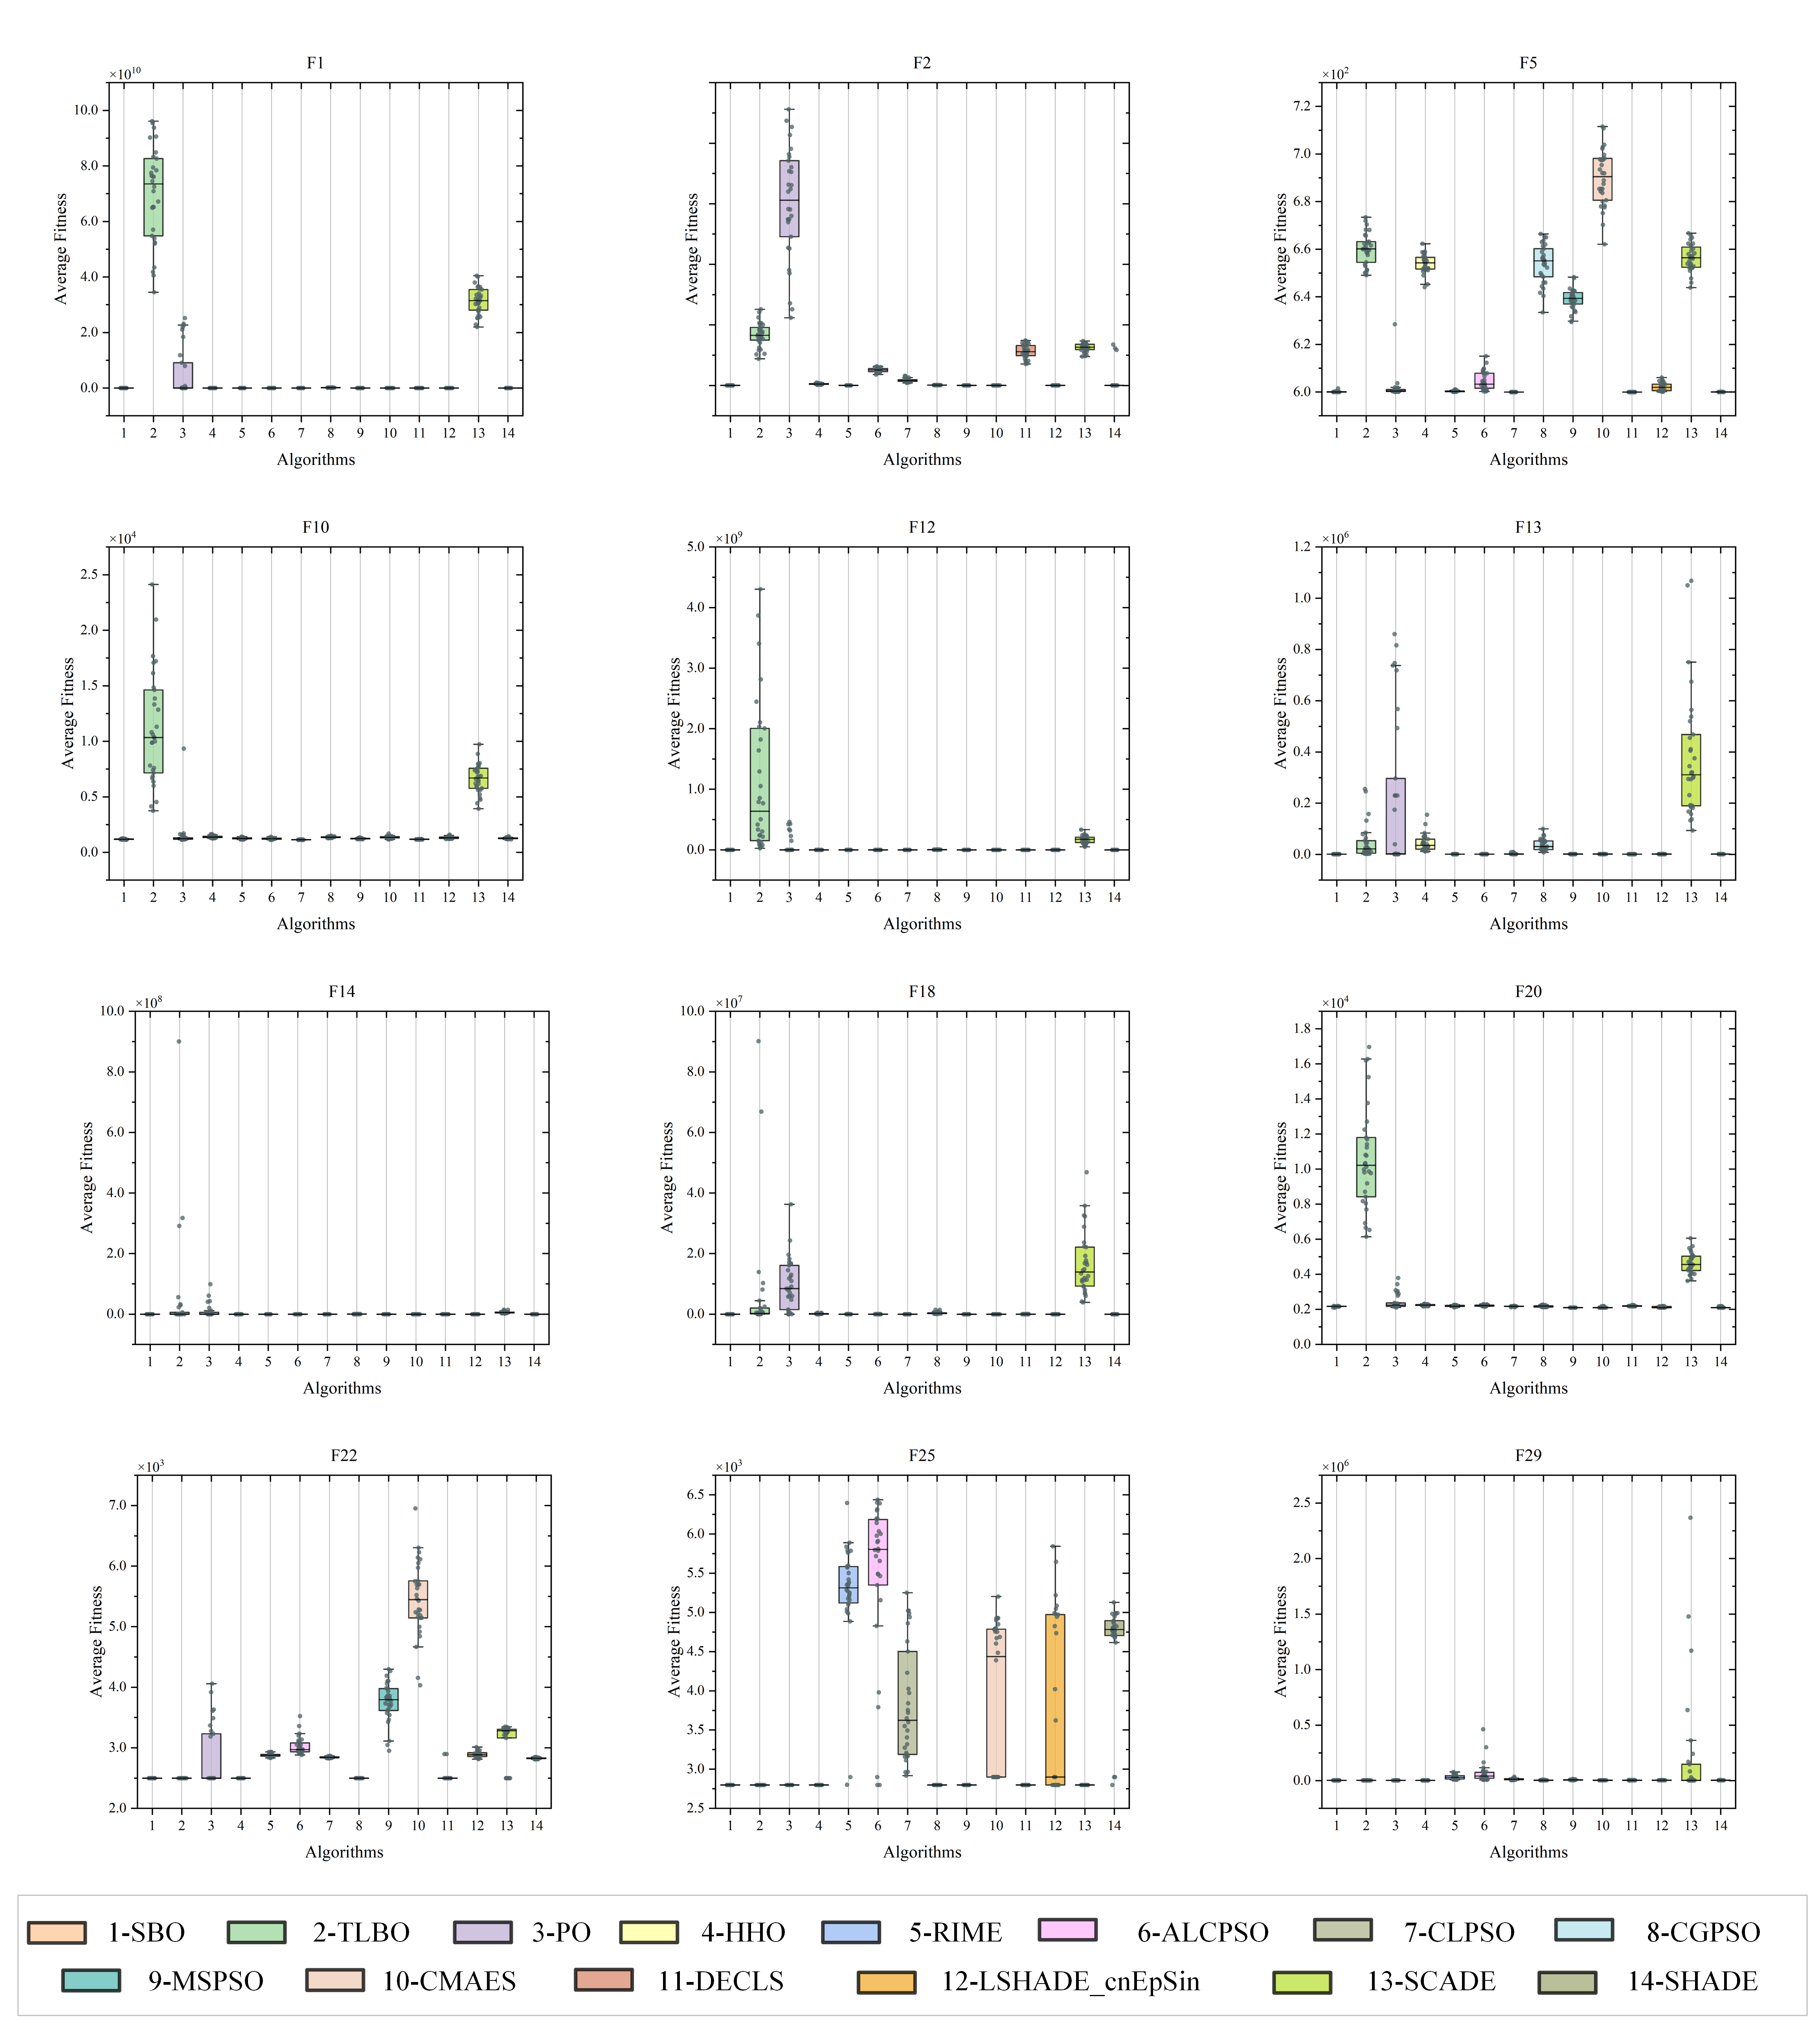
\includegraphics[width=\textwidth]{figures/chapter4/fig09_box_plots_30dim.png}
  \bicaption{SBO与先进算法在30维问题上的箱线图比较}{Box plots comparing SBO and state-of-the-art algorithms for 30-dimensional problems.}
  \label{fig:box_plots_30dim}
\end{figure}



统计分析进一步验证了SBO的竞争优势。如图10所示，Friedman检验结果表明SBO在所有维度上获得了最低的平均排名，10、30、50和100维度的值分别为3.90、4.07、4.38和4.48。这些排名突显了SBO的可扩展性及其在不同问题复杂度下持续良好表现的能力。表3中总结的Wilcoxon符号秩检验结果显示，SBO在超过70\%的基准函数中优于TLBO、PO、HHO和RIME，p值低于显著性阈值（$\alpha = 0.05$）。虽然其相对于LSHADE\_cnEpSin和LSHADE的优势不太明显，但SBO保持了竞争力，在部分函数中优于它们。



\begin{figure}[htbp]
  \centering
  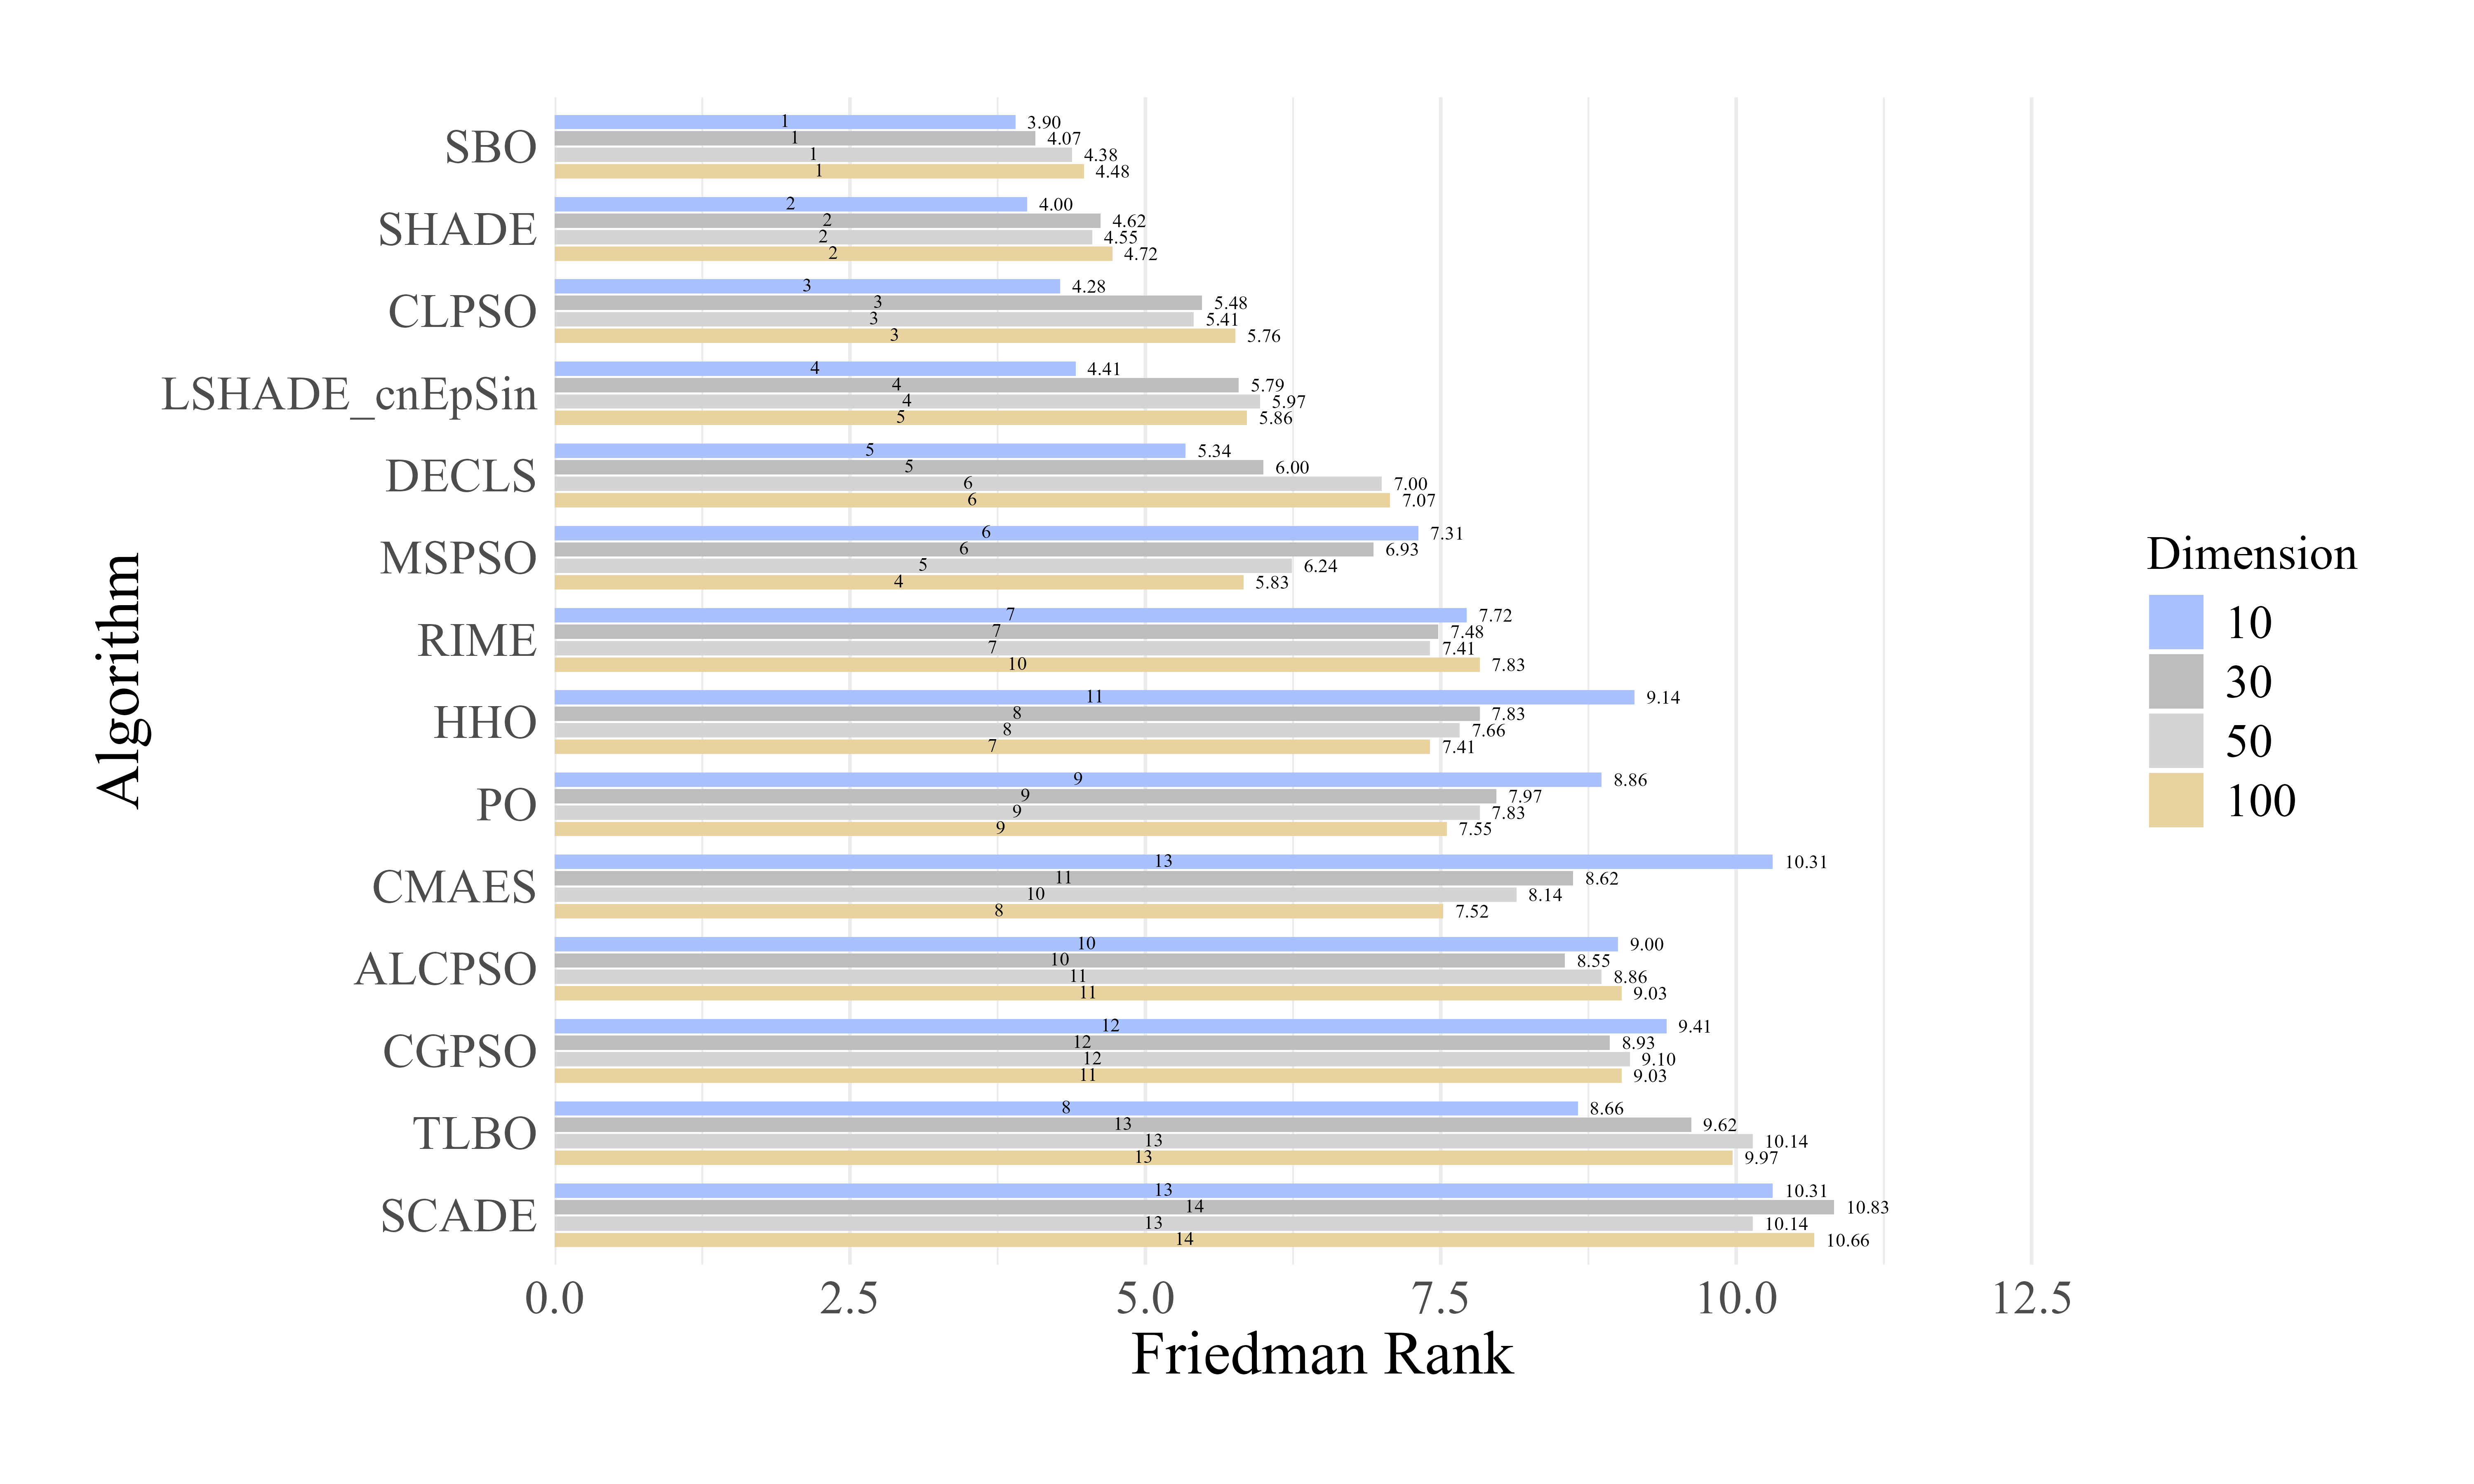
\includegraphics[width=\textwidth]{figures/chapter4/fig10_friedman_rank.png}
  \bicaption{四个维度下算法的Friedman排名结果}{Friedman rank result of algorithms across four dimensions.}
  \label{fig:friedman_rank}
\end{figure}



SBO算法的卓越性能源于其对寻求地位的社会行为的忠实建模，特别是向高性能同伴学习和战略性保留有益信息。这些机制使SBO能够在探索和开发之间实现有效平衡，使其在低维和高维问题中均能表现良好。SBO的资源保留策略特别为其在混合函数和组合函数中提供了优势，实现了快速收敛和跨不同运行的显著稳定性。尽管SBO在单峰函数上的性能略低于精度优先算法，但其整体适应性、稳定性和可扩展性使其成为多种优化任务的高效解决方案。

\noindent 

\begin{tabular}{|p{0.5in}|p{0.3in}|p{0.4in}|p{0.4in}|p{0.4in}|p{0.4in}|p{0.8in}|p{0.4in}|p{0.4in}|} \hline 
\multicolumn{9}{|p{1in}|}{\textbf{Table }3\textbf{. }WSRT and FT results of SBO and other algorithms on IEEE CEC 2017.} \\ \hline 
Dimension & Item & SBO & TLBO & PO & HHO & RIME & ALCPSO & CLPSO \\ \hline 
10 & \textbf{+/-/=} & $\mathrm{\sim}$ & 22/0/7 & 18/2/9 & 21/1/7 & 18/6/5 & 18/3/8 & 14/13/2 \\ \hline 
 & Rank\textbf{} & \textbf{3.8966} & 8.6552 & 8.8621 & 9.1379 & 7.7241 & 9.0000 & 4.2759 \\ \hline 
 & Result\textbf{} & \textbf{1} & 8 & 9 & 11 & 7 & 10 & 3 \\ \hline 
30 & \textbf{+/-/=} & $\mathrm{\sim}$\textbf{} & 21/0/8 & 16/2/11 & 21/0/8 & 20/7/2 & 21/4/4 & 15/11/3 \\ \hline 
 & Rank\textbf{} & \textbf{4.0690} & 9.6207 & 7.9655 & 7.8276 & 7.4828 & 8.5517 & 5.4828 \\ \hline 
 & Result\textbf{} & \textbf{1} & 13 & 9 & 8 & 7 & 10 & 3 \\ \hline 
50 & \textbf{+/-/=} & $\mathrm{\sim}$\textbf{} & 21/0/8 & 16/5/8 & 21/0/8 & 17/7/5 & 20/5/4 & 12/13/4 \\ \hline 
 & Rank\textbf{} & \textbf{4.3793} & 10.1379 & 7.8276 & 7.6552 & 7.4138 & 8.8621 & 5.4138 \\ \hline 
 & Result\textbf{} & \textbf{1} & 13 & 9 & 8 & 7 & 11 & 3 \\ \hline 
100 & \textbf{+/-/=} & $\mathrm{\sim}$ & 21/0/8 & 14/5/10 & 21/0/8 & 16/6/7 & 18/5/6 & 13/14/2 \\ \hline 
 & Rank\textbf{} & \textbf{4.4828} & 9.9655 & 7.5517 & 7.4138 & 7.8276 & 9.0345 & 5.7586 \\ \hline 
 & Result\textbf{} & \textbf{1} & 13 & 9 & 7 & 10 & 11 & 3 \\ \hline 
Dimension & Item & CGPSO & MSPSO & CMAES & DECLS & LSHADE\_cnEpSin & SCADE & SHADE \\ \hline 
10 & \textbf{+/-/=} & 28/1/0 & 23/3/3 & 24/1/4 & 14/10/5 & 10/9/10 & 23/0/6 & 8/16/5 \\ \hline 
 & Rank & 9.4138 & 7.3103 & 10.3103 & 5.3448 & 4.4138 & 10.3103 & 4.0000 \\ \hline 
 & Result & 12 & 6 & 13 & 5 & 4 & 13 & 2 \\ \hline 
30 & \textbf{+/-/=} & 27/0/2 & 20/5/4 & 21/6/2 & 18/7/4 & 14/14/1 & 24/0/5 & 14/14/1 \\ \hline 
 & Rank & 8.9310 & 6.9310 & 8.6207 & 6.0000 & 5.7931 & 10.8276 & 4.6207 \\ \hline 
 & Result & 12 & 6 & 11 & 5 & 4 & 14 & 2 \\ \hline 
50 & \textbf{+/-/=} & 29/0/0 & 14/10/5 & 19/9/1 & 20/5/4 & 12/12/5 & 23/0/6 & 13/16/0 \\ \hline 
 & Rank & 9.1034 & 6.2414 & 8.1379 & 7.0000 & 5.9655 & 10.1379 & 4.5517 \\ \hline 
 & Result & 12 & 5 & 10 & 6 & 4 & 13 & 2 \\ \hline 
100 & \textbf{+/-/=} & 28/1/0 & 13/15/1 & 18/10/1 & 21/6/2 & 13/13/3 & 24/0/5 & 11/17/1 \\ \hline 
 & Rank & 9.0345 & 5.8276 & 7.5172 & 7.0690 & 5.8621 & 10.6552 & 4.7241 \\ \hline 
 & Result & 11 & 4 & 8 & 6 & 5 & 14 & 2 \\ \hline 
\end{tabular}




\subsection{运行时间性能分析}

为全面评估所提SBO算法的运行时间性能，本文使用包含29个不同函数的IEEE CEC 2017基准测试套件进行了实验。每种算法，包括SBO和13种最先进的竞争算法，在四个维度（10、30、50和100）下对每个基准函数独立执行30次。运行时间性能以每个维度下29个函数30次运行的平均运行时间（秒）来衡量。结果总结在表4中并在图11中可视化。

纳入比较的算法包括TLBO、PO、HHO、物理启发算法RIME、四种PSO变体（ALCPSO、CLPSO、CGPSO和MSPSO）以及五种进化算法（CMAES、DECLS、LSHADE\_cnEpSin、SCADE和SHADE）。

运行时间结果表明SBO在所有测试维度上均展现出有竞争力的性能。在最小维度（$D=10$）下，SBO获得第二快的运行时间（28.08秒），仅落后于CGPSO（27.57秒）。随着问题维度的增加，SBO始终排名为最快的算法，在维度$D=30$、$D=50$和$D=100$下获得最短运行时间，平均运行时间分别为74.25、151.24和478.73秒。

与LSHADE\_cnEpSin和SCADE等较慢的算法相比，SBO展现出显著更好的可扩展性。结果表明SBO的计算效率在更高维度下愈加显著。这一改善归因于SBO采用的高效机制，减少了资源评估和更新过程中不必要的计算开销。

图11中的可视化突显了SBO在各维度下的运行时间性能，展示了其一致性和可扩展性。虽然TLBO和ALCPSO等算法仍具竞争力，但SBO在更高维度下的优越运行时间证实了其对大规模优化任务的适用性。

尽管有这些发现，需要注意的是，由于硬件和软件配置的差异，运行时间性能可能因计算环境而异。未来的研究将致力于在不同平台上标准化额外的运行时间评估，以进一步验证这些结果。

\noindent 

\noindent \textbf{Table }4\textbf{. }Runtime performance of SBO and other algorithms on IEEE CEC 2017.

\begin{tabular}{|p{0.5in}|p{0.4in}|p{0.4in}|p{0.4in}|p{0.4in}|p{0.8in}|p{0.4in}|p{0.4in}|} \hline 
Dimension & SBO & TLBO & PO & HHO & RIME & ALCPSO & CLPSO \\ \hline 
10 & 28.08  & 32.07  & 60.36  & 59.10  & 48.11  & 39.17  & 39.92  \\ \hline 
30 & \textbf{74.25 } & 77.67  & 101.20  & 107.86  & 88.65  & 92.48  & 107.64  \\ \hline 
50 & \textbf{151.24 } & 155.10  & 190.04  & 217.82  & 175.12  & 157.99  & 181.29  \\ \hline 
100 & \textbf{478.73 } & 483.49  & 551.37  & 683.48  & 531.06  & 496.47  & 535.68  \\ \hline 
Dimension & CGPSO & MSPSO & CMAES & DECLS & LSHADE\_cnEpSin & SCADE & SHADE \\ \hline 
10 & \textbf{27.57 } & 81.57  & 67.94  & 32.75  & 94.44  & 57.67  & 42.16  \\ \hline 
30 & 112.18  & 128.53  & 111.10  & 101.04  & 179.70  & 135.75  & 92.36  \\ \hline 
50 & 180.14  & 160.21  & 177.28  & 182.29  & 248.05  & 259.45  & 176.46  \\ \hline 
100 & 577.42  & 486.66  & 522.08  & 515.72  & 636.77  & 770.86  & 520.70  \\ \hline 
\end{tabular}



\begin{figure}[htbp]
  \centering
  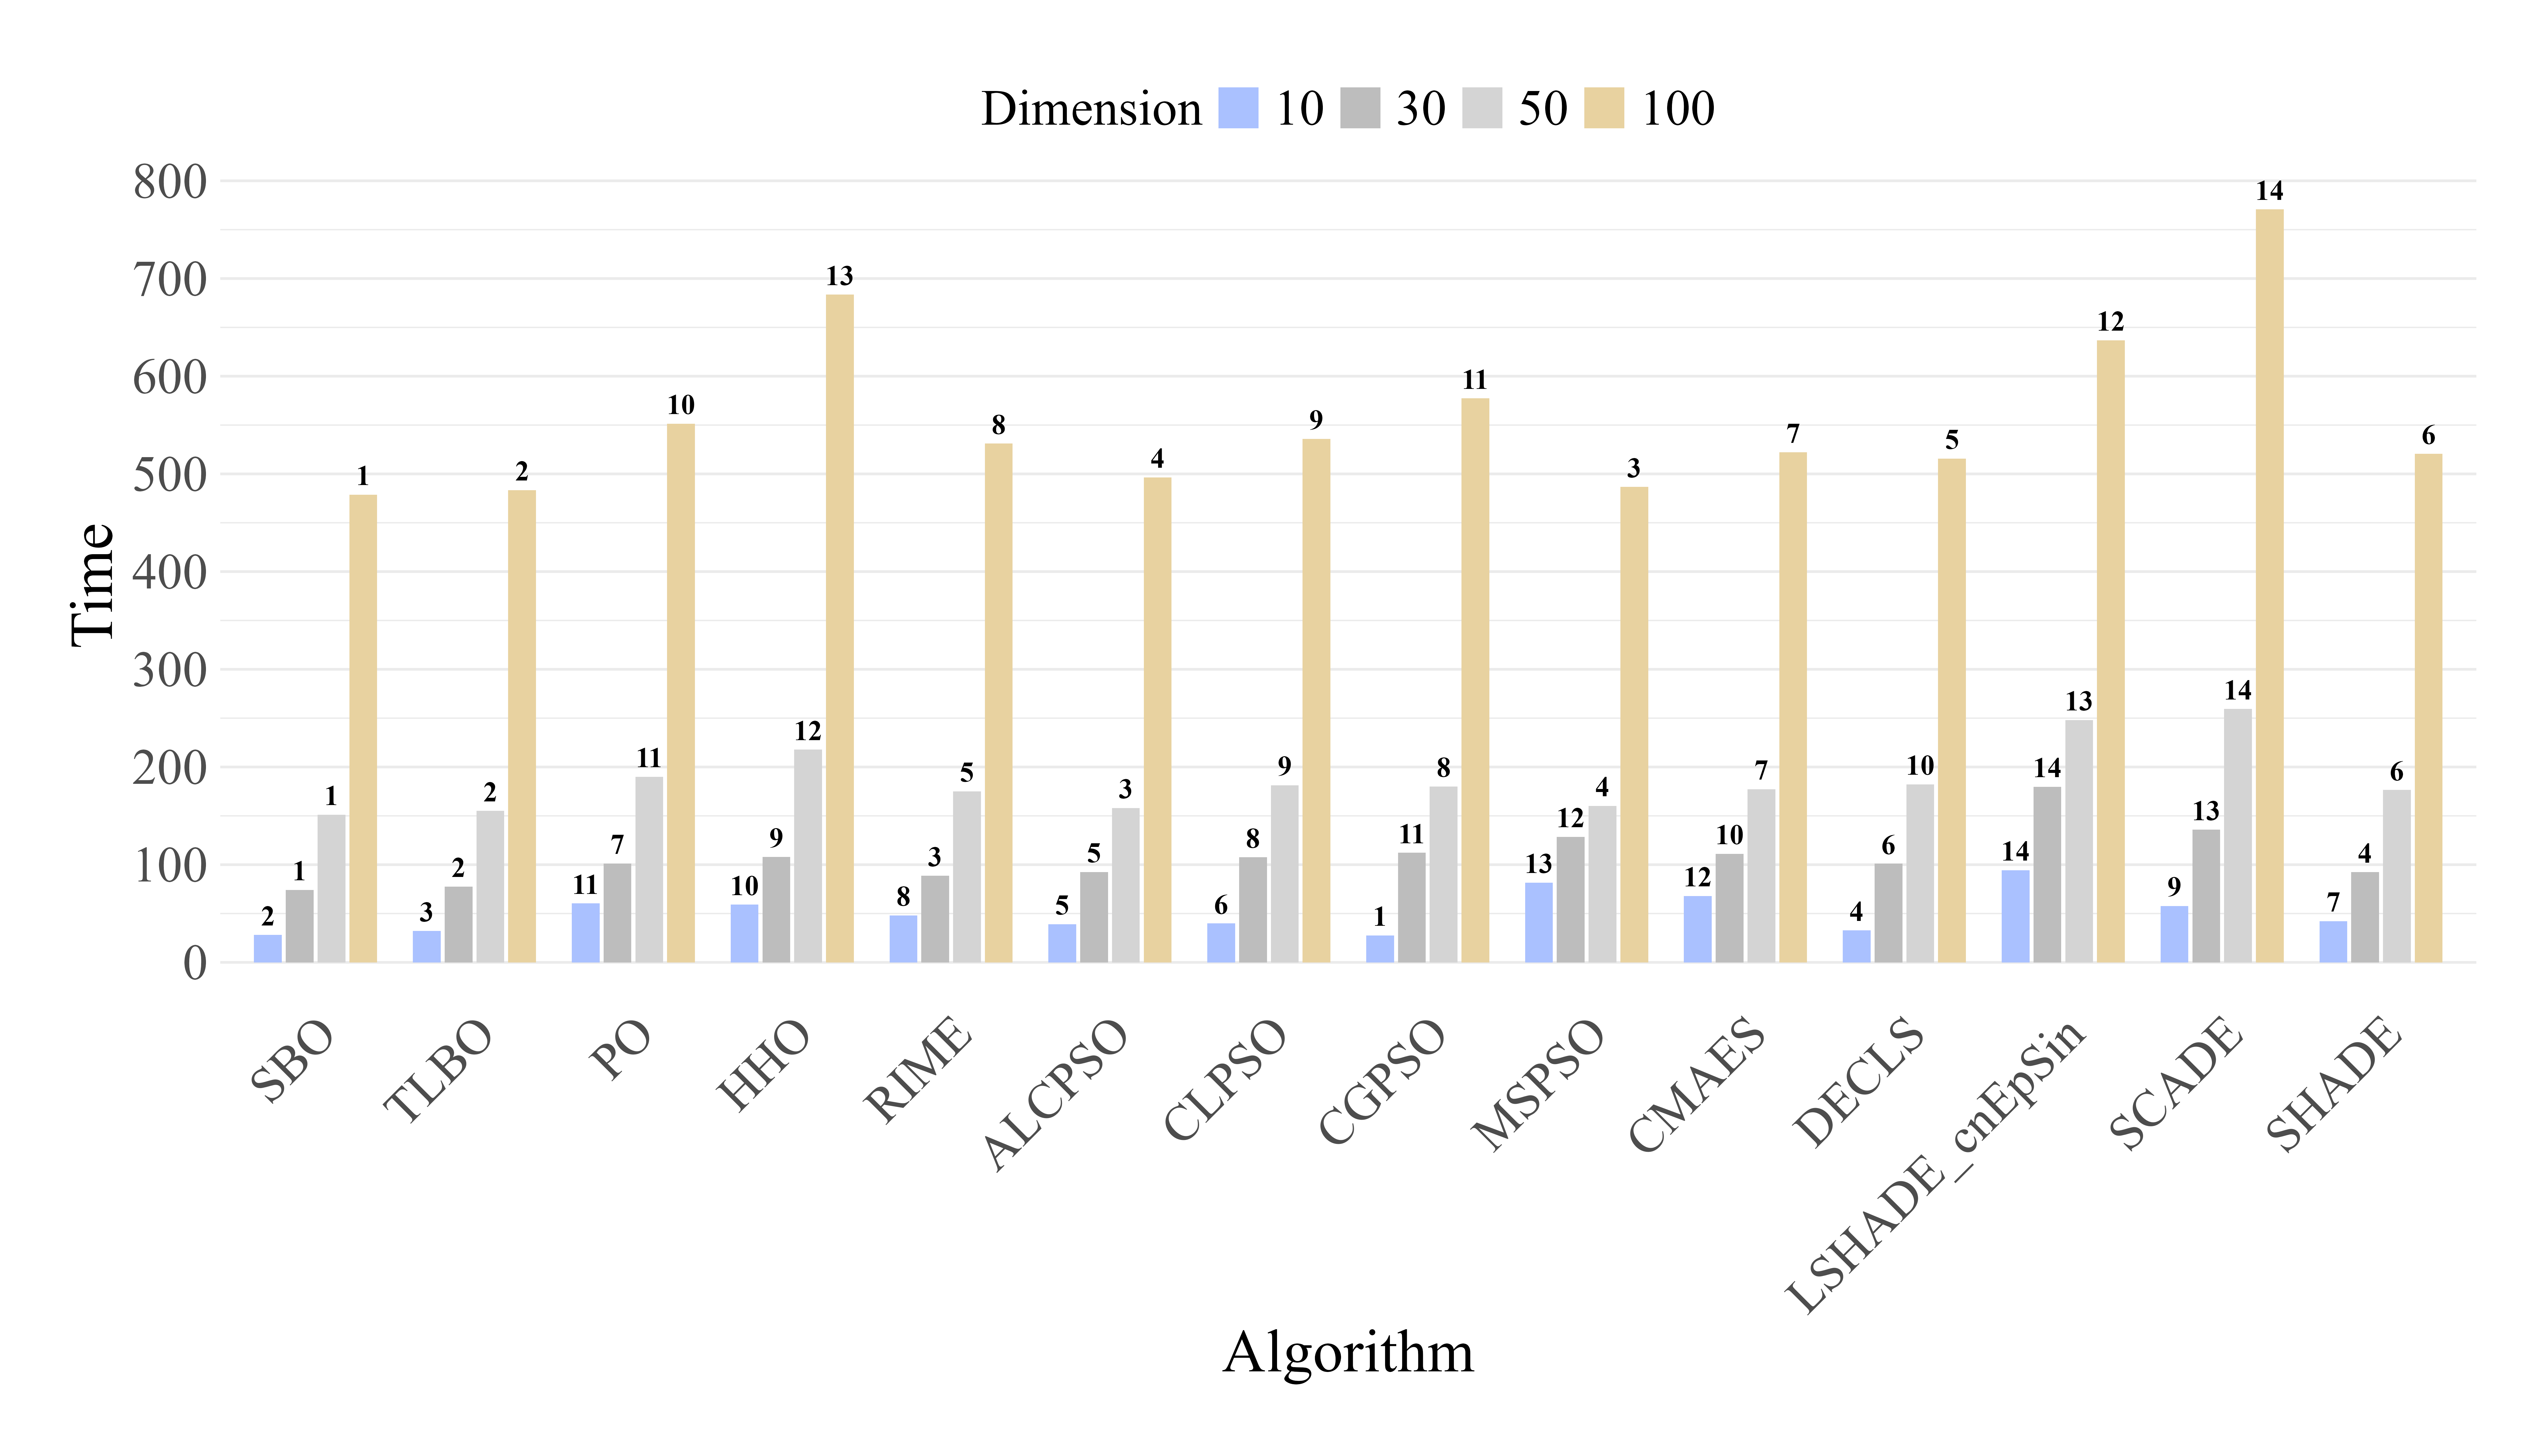
\includegraphics[width=\textwidth]{figures/chapter4/fig11_runtime_performance.png}
  \bicaption{SBO与其他算法在IEEE CEC 2017上的运行时间性能}{Runtime performance of SBO with other algorithms on IEEE CEC 2017.}
  \label{fig:runtime_performance}
\end{figure}




\section{实验验证}

本节将SBO框架应用于两个重要的优化应用：特征选择和多阈值图像分割。为解决特征选择这一经典离散优化挑战，将SBO转换为其二值变体bSBO。这一改编建立在SBO在连续空间全局优化中已证明的效率基础上，支持了其在离散应用中的潜力。bSBO旨在通过选择最相关的属性同时消除冗余来优化特征选择，从而通过最优特征选择提高预测模型性能。随后将所提bSBO与KNN分类器结合以验证性能。最后，bSBO在9个高维UCI数据集上与8种最先进的二值优化器进行基准测试，证明了其在离散优化中的竞争优势。

超越特征选择，本文还评估了SBO在多阈值图像分割中的性能——这是一项需要精确阈值确定以实现准确图像分析的连续优化任务。在该评估中，SBO使用来自浸润性导管癌（Invasive Ductal Carcinoma，IDC）数据集的9张乳腺癌组织学图像与7种先进的元启发式算法进行竞争，以衡量分割质量的改善。通过保持最优的探索-开发平衡，SBO证明了其在离散和连续问题域中的高度适应性，确认了其在各种现实世界优化挑战中的通用性。




\subsection{特征选择}

特征选择是数据集分析中的关键过程，涉及挑选最有影响力和最重要的特征以降低数据维度，并忽略冗余和不相关的属性\cite{sbo_ref61}。这种选择性提取不仅增强了基于这些特征训练的模型的泛化性和鲁棒性，还提高了计算效率。目前主要有三种公认的特征选择方法：过滤法（Filter Method）\cite{sbo_ref62}、嵌入法（Embedded Method）\cite{sbo_ref63}和包裹法（Wrapper Method）\cite{sbo_ref64}——每种方法都具有不同的选择流程。

过滤法使用统计度量评估特征相关性，如用于线性特征-目标关系的Pearson相关系数\cite{sbo_ref65}、用于信息增益的卡方检验\cite{sbo_ref66}以及用于丢弃低方差特征的方差阈值法\cite{sbo_ref67}。这些评估独立于机器学习算法。相比之下，嵌入法在模型训练阶段内在地进行选择，将特征重要性评估集成到优化过程中，流行的技术包括Lasso回归\cite{sbo_ref68}（即L1正则化，通过惩罚回归系数的绝对值将不重要的特征系数归零）和基于树的方法\cite{sbo_ref69}（自动确定特征重要性）。与以上两种方法不同，包裹法通过迭代模型训练评估特征子集，选择基于评估指标最大化性能的子集，使该方法计算量更大但通常更准确。

本文特别关注bSBO——一种迭代搜索最优特征子集的MA，通过基于适应度函数的评估指标进行评估。鉴于每增加一个特征，潜在特征组合呈指数增长，像所提bSBO这样的MAs对于管理特征选择问题的组合特性非常有帮助，因此使基于包裹法的特征选择在当前数据集降维实践中日益流行。


\subsubsection{基于bSBO的包裹式方法}

本节介绍将KNN分类器（K设为5）与bSBO集成的基于包裹法的特征选择方法。图12中的详细流程图概述了选择有效特征子集的过程。

适应度函数的设计旨在实现最小化选择特征数量与降低分类器错误率之间的权衡。设$E$表示KNN分类器的错误率，$|S|$表示bSBO选择的特征数量，$|A|$表示数据集中的总特征数量。适应度函数定义如式~\eqref{sbo_eq_17}所示。参数设置为$α=0.05$和$β=0.95$，确保更多的权重放在错误率上。该公式引导优化器偏向在选择紧凑特征子集的同时保持高预测精度的解。

\begin{equation}
\label{sbo_eq_17}
f_{obj}=α\times E+β\times \frac{\left|S\right|}{\left|A\right|}
\end{equation}



该过程从数据预处理开始。数据集被分为十折并归一化到[$\mathrm{-}$1,1]范围。每个候选解表示为连续值向量，然后转换为二值决策以指示是否选择某个特征。这种转换通过V型转换函数实现，定义为：

\begin{equation}
\label{sbo_eq_18}
T\left(x_{i,j}\right)=\left|erf\left(sqrt\left(\frac{π}{2}\right)\times x_{i,j}\right)\right|
\end{equation}

\begin{equation}
\label{sbo_eq_19}
erf\left(x\right)=\frac{2}{sqrt\left(π\right)}\int^x_0{e^{-t^2}}dt
\end{equation}

其中$x_{i,j}$是第$ith$个候选解第$jth$分量的连续值。结果值以0.5为阈值产生特征选择的二值决策。

转换后，每个候选解对应一个长度为$D$的二值向量，表示数据集的维度。选定的特征子集用于在训练数据上训练KNN分类器，其性能在测试集上评估以计算错误率$E$。

bSBO在固定迭代次数内迭代更新候选解。每次迭代都评估适应度函数，并相应精炼候选特征子集。优化过程结束后，使用表现最优的特征子集训练最终的KNN模型，并在测试数据集上评估其预测精度。

基于bSBO方法的性能通过考虑三个指标来评估：多次试验的平均适应度值、KNN分类器的错误率和选择的特征数量。这些指标全面评估了该方法在实现模型精度和特征缩减两方面的能力。与八种最先进的二值优化器的比较分析进一步证明了所提方法在产生鲁棒且可解释模型方面的有效性。

\noindent 

\begin{figure}[htbp]
  \centering
  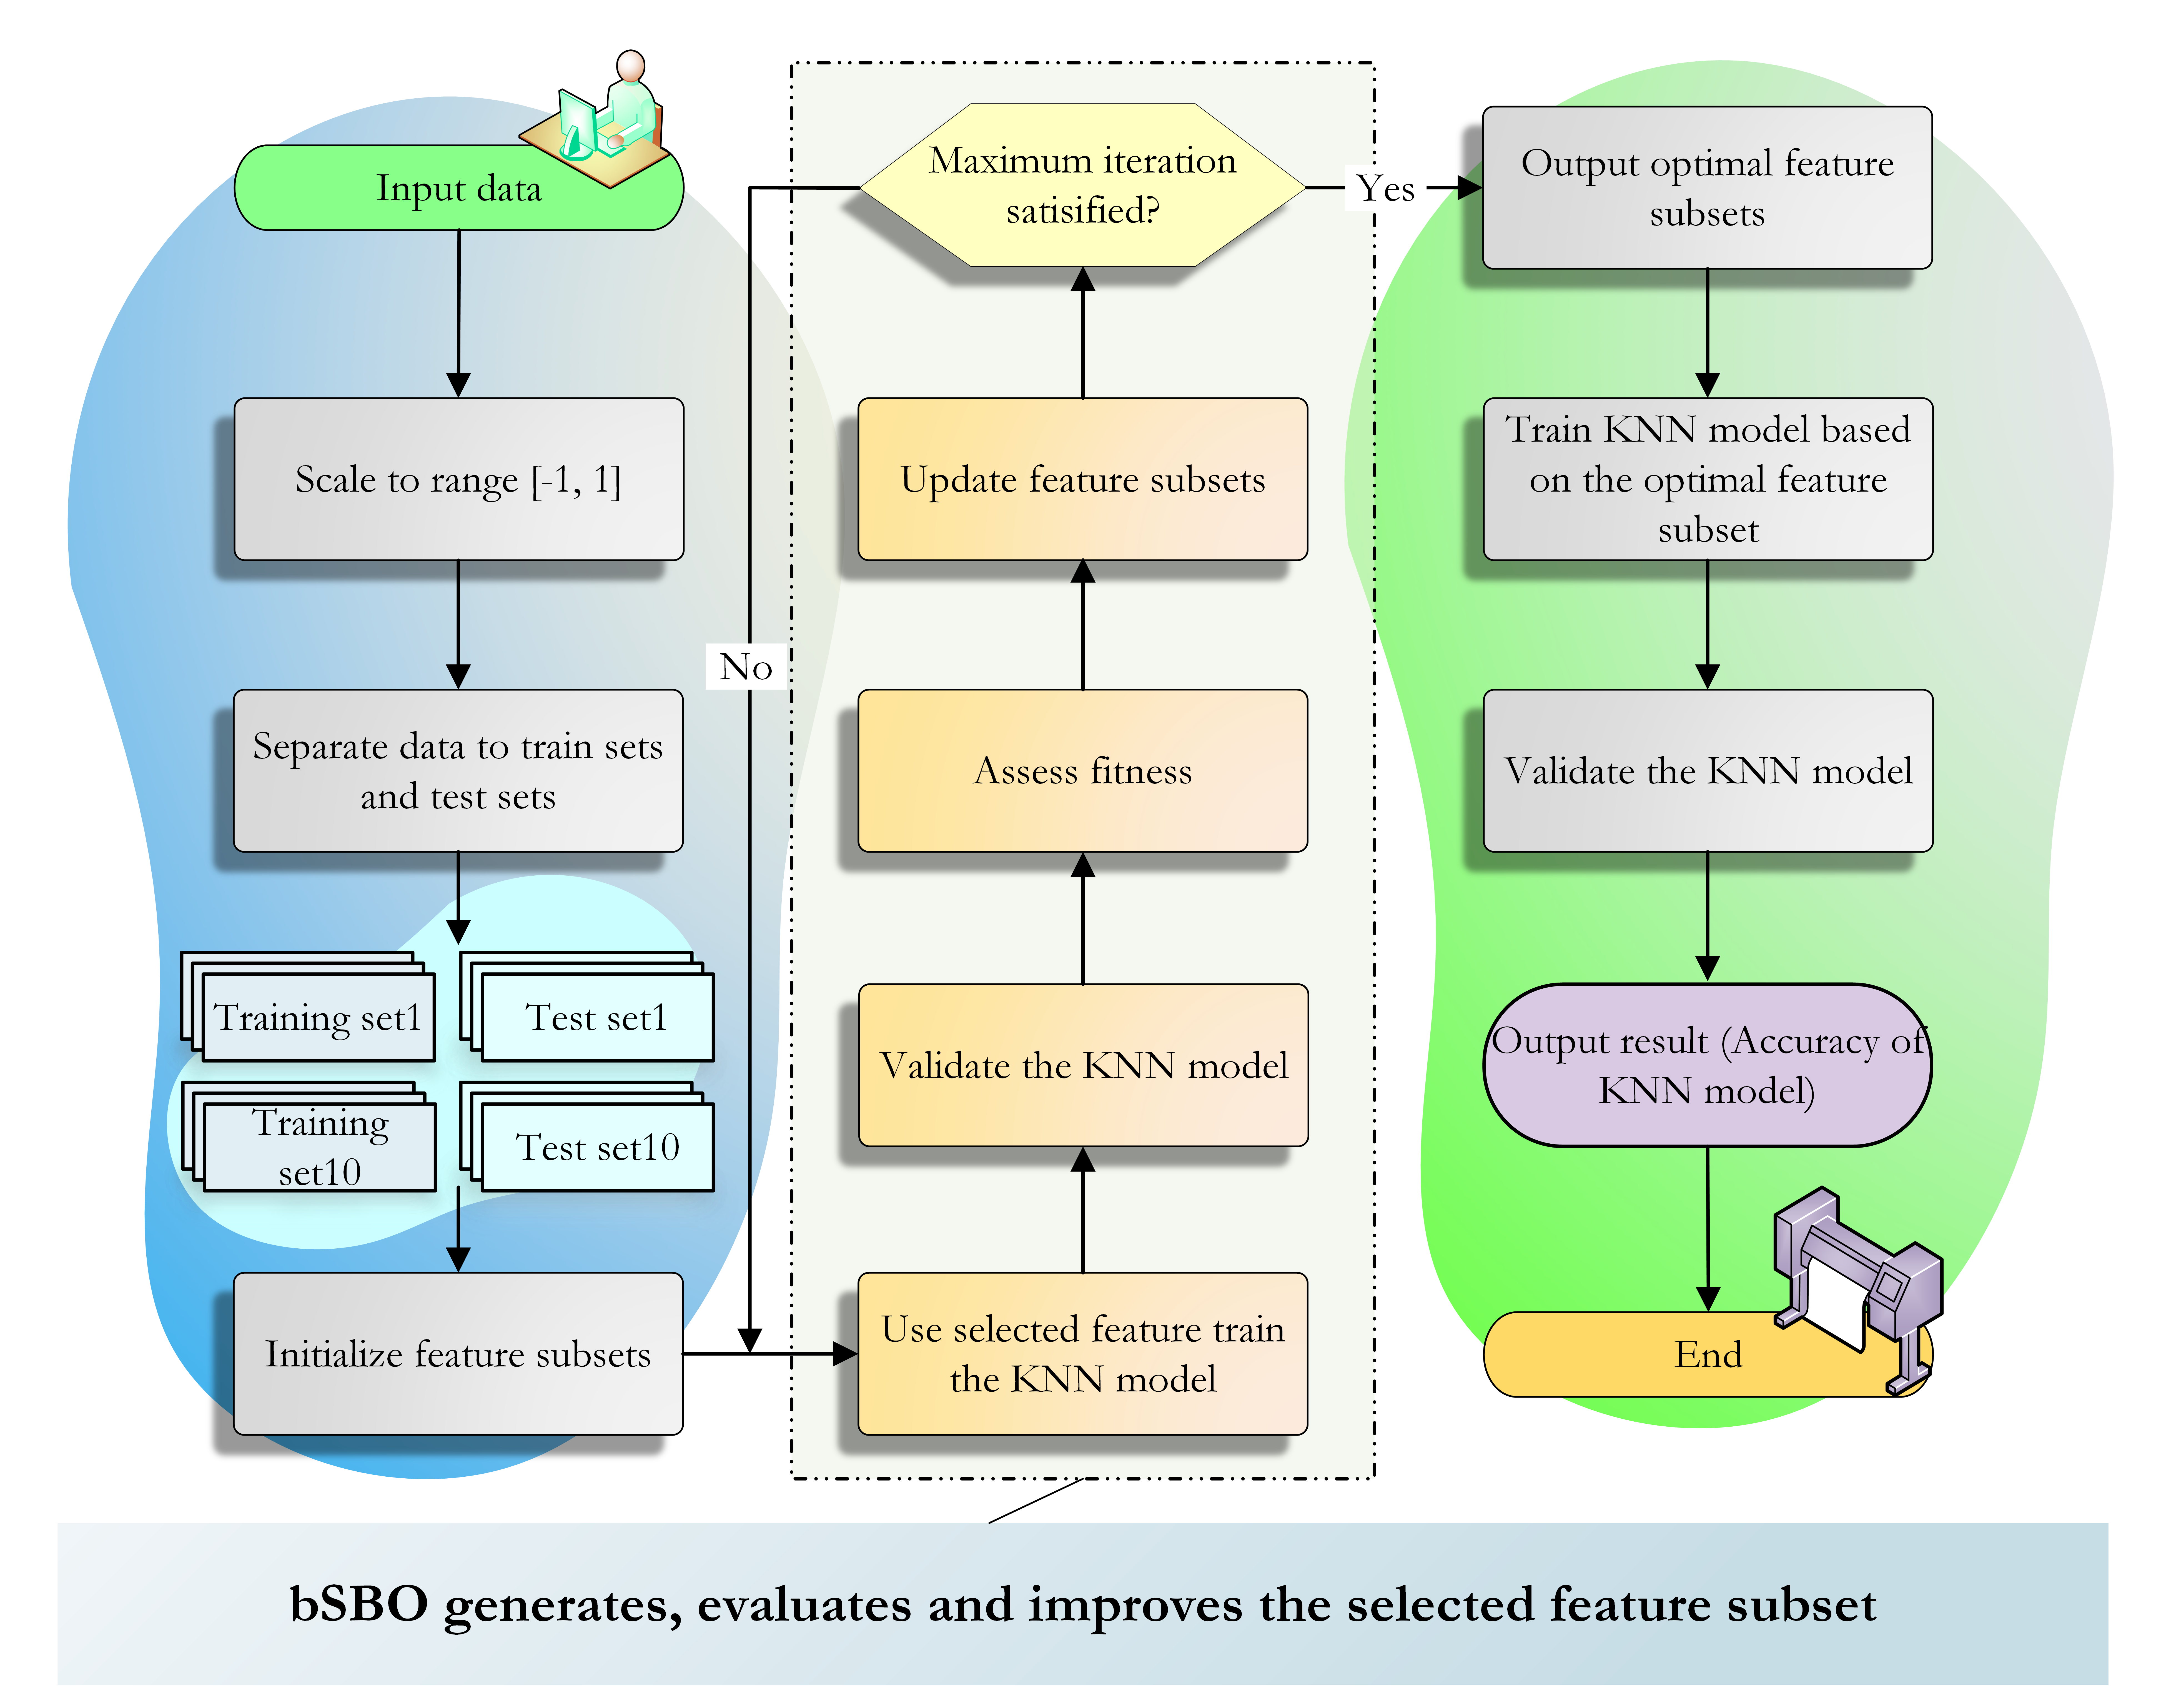
\includegraphics[width=\textwidth]{figures/chapter4/fig12_flowchart_bSBO_wrapper.png}
  \bicaption{基于bSBO的包裹式特征选择方法流程图}{Flowchart of bSBO-based wrapper method for feature selection.}
  \label{fig:flowchart_bSBO_wrapper}
\end{figure}




\subsubsection{bSBO的实验结果与分析}

本节专门通过将bSBO与八种最先进的二值优化器进行直接竞争来评估其优化能力。这些比较算法包括二值飞蛾火焰优化器（bMFO）\cite{sbo_ref70}、bGWO\cite{sbo_ref71}、bGSA\cite{sbo_ref72}、bPSO\cite{sbo_ref73}、二值蚁狮优化器（bALO）\cite{sbo_ref74}、二值蝙蝠算法（bBA）\cite{sbo_ref75}、二值樽海鞘群算法（bSSA）\cite{sbo_ref76}和bHHO\cite{sbo_ref77}。每个优化器的控制参数遵循其原始出版物。

为此比较选择的数据集具有多样性和代表性，如表5所示，来自UCI机器学习库，维度从2,308到12,600不等，确保了全面的基准测试。此外，类别数量（从两类到四类）和样本量（每个数据集从50到203）的变化为评估bSBO在各种复杂数据环境中相对于现有二值优化器的优化能力提供了鲁棒的框架。



\begin{tabular}{|p{1.0in}|p{1.0in}|p{1.0in}|p{1.0in}|} \hline 
\multicolumn{4}{|p{1in}|}{\textbf{Table }5\textbf{.} Description of the used high-dimensional datasets.} \\ \hline 
Dataset & Samples & Features & Classes \\ \hline 
Brain\_Tumor2 & 50 & 10367 & 4 \\ \hline 
CNS & 60 & 7129 & 2 \\ \hline 
DLBCL & 77 & 5469 & 2 \\ \hline 
Leukemia & 72 & 7130 & 2 \\ \hline 
Leukemia1 & 72 & 5327 & 3 \\ \hline 
Leukemia2 & 72 & 11225 & 3 \\ \hline 
Lung\_Cancer & 203 & 12600 & 3 \\ \hline 
Prostate\_Tumor & 102 & 10509 & 2 \\ \hline 
SRBCT & 83 & 2308 & 4 \\ \hline 
\end{tabular}



为在所有优化算法之间标准化条件，实验设计设定了最大50次迭代的终止准则和20的种群大小。为减轻随机性对结果的影响，每个优化器对每个数据集运行10次。此外，为评估训练模型的性能，对每个数据集采用10折交叉验证\cite{sbo_ref78}，这是一种广泛认可的确保机器学习模型有效性的方法。

这些实验的结果在表6至表8中展示，提供了bSBO和其他八种二值优化器在适应度值、所选特征数量和错误率方面的比较数据。为定量确立bSBO相对于其竞争对手的优越性，对结果进行了Wilcoxon符号秩检验和Friedman检验的统计分析。选择这些非参数检验是因为它们能够检测配对观测之间的显著差异，并能够在多个数据集上比较两个以上的算法，分别为比较分析提供了鲁棒的统计框架。

表6展示了适应度值的详细比较，揭示了bSBO在与其他八种二值优化器比较时在所有九个数据集上获得了最低的适应度分数。然而，需要注意某些偏差，特别是Leukemia2、Lung\_Cancer和Prostate\_Tumor数据集的较高Std值，其中bSBO分别记录了比bHHO、bMFO和bHHO更大的Std值。

尽管存在这些Std值的差异，表6底部展示的统计检验有力地支持了bSBO的优越性能。它在所有数据集上决定性地优于其他八种优化器，以排名值1获得了榜首位置。这使bSBO明显领先于其最接近的竞争对手bHHO，后者获得了排名值2.25的次优位置。这些统计检验的纳入验证了bSBO在实验数据集中优化适应度值方面领先地位的鲁棒性。



\begin{tabular}{|p{0.4in}|p{0.4in}|p{0.4in}|p{0.4in}|p{0.4in}|p{0.4in}|p{0.4in}|p{0.4in}|p{0.4in}|p{0.4in}|p{0.4in}|} \hline 
\multicolumn{11}{|p{1in}|}{\textbf{Table }6\textbf{. }Comparative results of average fitness values between bSBO and other binary optimizers.\textbf{}} \\ \hline 
Dataset & Metric & bSBO & bMFO & bGWO & bGSA & bPSO & bALO & bBA & bSSA & bHHO \\ \hline 
Brain\_Tumor2 & Std & \textbf{3.80E-06} & 1.83E-04 & 6.00E-02 & 1.12E-01 & 1.18E-01 & 9.62E-02 & 2.30E-01 & 8.49E-02 & 8.82E-02 \\ \hline 
 & Avg & \textbf{9.65E-06} & 1.71E-04 & 5.74E-03 & 1.02E-01 & 2.39E-02 & 2.37E-02 & 2.04E-02 & 1.95E-02 & 9.27E-03 \\ \hline 
CNS & Std & \textbf{2.25E-05} & 2.25E-04 & 6.67E-02 & 7.91E-02 & 1.09E-01 & 8.34E-02 & 1.48E-01 & 1.31E-01 & 1.23E-04 \\ \hline 
 & Avg & \textbf{1.75E-05} & 2.77E-04 & 5.86E-03 & 2.32E-02 & 1.82E-01 & 1.70E-01 & 2.37E-01 & 1.04E-01 & 4.21E-05 \\ \hline 
DLBCL & Std & \textbf{7.21E-06} & 1.08E-04 & 2.80E-04 & 3.77E-02 & 3.75E-02 & 3.28E-04 & 3.70E-02 & 4.41E-02 & 1.88E-05 \\ \hline 
 & Avg & \textbf{1.83E-05} & 1.14E-04 & 5.33E-03 & 2.16E-02 & 2.34E-02 & 2.29E-02 & 2.14E-02 & 2.23E-03 & \textbf{1.83E-05} \\ \hline 
Leukemia & Std & \textbf{5.73E-06} & 6.30E-05 & 2.55E-04 & 1.97E-04 & 2.49E-04 & 2.12E-04 & 3.22E-03 & 8.97E-03 & 1.85E-05 \\ \hline 
 & Avg & \textbf{1.40E-05} & 7.71E-05 & 5.49E-03 & 2.18E-02 & 2.34E-02 & 2.30E-02 & 1.65E-02 & 2.40E-02 & 1.75E-05 \\ \hline 
Leukemia1 & Std & \textbf{6.07E-05} & 1.86E-04 & 3.53E-04 & 3.55E-04 & 2.06E-04 & 2.32E-04 & 4.23E-02 & 6.53E-03 & 1.06E-04 \\ \hline 
 & Avg & \textbf{1.88E-05} & 1.88E-04 & 5.28E-03 & 2.14E-02 & 2.31E-02 & 2.27E-02 & 1.79E-02 & 2.30E-02 & 5.16E-05 \\ \hline 
Leukemia2 & Std & 2.44E-05 & 8.46E-05 & 1.76E-04 & 3.60E-04 & 5.38E-02 & 5.38E-02 & 6.16E-02 & 5.90E-02 & \textbf{2.27E-05} \\ \hline 
 & Avg & \textbf{1.78E-05} & 1.45E-04 & 5.43E-03 & 2.25E-02 & 2.37E-02 & 2.35E-02 & 1.76E-02 & 2.42E-02 & 3.12E-05 \\ \hline 
Lung\_Cancer & Std & 4.02E-04 & \textbf{3.11E-04} & 2.11E-02 & 3.41E-02 & 3.41E-02 & 2.23E-02 & 4.27E-02 & 3.13E-02 & 2.30E-02 \\ \hline 
 & Avg & \textbf{8.13E-05} & 5.58E-04 & 6.01E-03 & 4.45E-02 & 4.68E-02 & 2.39E-02 & 4.29E-02 & 3.86E-02 & 8.64E-03 \\ \hline 
Prostate\_Tumor & Std & 6.37E-05 & 1.89E-04 & 2.99E-02 & 4.80E-02 & 7.66E-02 & 4.80E-02 & 9.69E-02 & 5.15E-02 & \textbf{5.22E-05} \\ \hline 
 & Avg & \textbf{2.62E-05} & 2.47E-04 & 6.19E-03 & 2.30E-02 & 2.42E-02 & 2.38E-02 & 1.11E-01 & 6.77E-02 & 7.14E-05 \\ \hline 
SRBCT & Std & \textbf{7.81E-05} & 1.04E-04 & 2.85E-04 & 4.19E-04 & 3.74E-02 & 3.50E-04 & 4.82E-02 & 4.93E-02 & 1.50E-04 \\ \hline 
\textbf{} & Avg & \textbf{1.08E-04} & 1.95E-04 & 4.15E-03 & 1.95E-02 & 2.22E-02 & 2.16E-02 & 1.73E-02 & 2.24E-02 & 1.19E-04 \\ \hline 
\textbf{+/-/=} & $\mathrm{\sim}$ & $\mathrm{\sim}$ & 9/0/0 & 9/0/0 & 9/0/0 & 9/0/0 & 9/0/0 & 9/0/0 & 9/0/0 & 8/1/0 \\ \hline 
Friedman-rank &  & 1.00  & 2.88  & 3.88  & 5.88  & 7.88  & 6.63  & 8.38  & 6.25  & 2.25  \\ \hline 
Result &  & 1 & 3 & 4 & 5 & 8 & 7 & 9 & 6 & 2 \\ \hline 
\end{tabular}



表7和表8显示了关于所选特征数量以及使用这些特征训练的机器学习模型对应错误率的结果。这些表格底部还包含非参数统计结果，以提供深入的分析见解。研究结果表明，bSBO不仅选择了最少的特征数量，还在九个数据集上实现了最低的错误率。根据所选特征数量和错误率的排名，bSBO始终以排名1获得榜首位置。

在表7中，可以观察到Leukemia2、Lung\_Cancer和Prostate\_Tumor数据集对应的Std值较大，但在比较bSBO与bHHO、bGSA和bHHO时Std值的差异很小，这突显了bSBO的一致性和鲁棒性。

为了增强对bSBO相对于其他优化器鲁棒性能的可视化解读和比较分析，图13使用柱状图展示了Friedman排名结果。该可视化清晰地描绘了不同优化器在多个评估指标上的相对性能。排名越低表示性能越好，bSBO获得了最有利的排名，从而证明了其持续的优越性。



\begin{tabular}{|p{0.4in}|p{0.4in}|p{0.4in}|p{0.4in}|p{0.4in}|p{0.4in}|p{0.4in}|p{0.4in}|p{0.4in}|p{0.4in}|p{0.4in}|} \hline 
\multicolumn{11}{|p{1in}|}{\textbf{Table }7\textbf{. }Comparative results of average selected feature numbers between bSBO and other binary optimizers.\textbf{}} \\ \hline 
Dataset & Metric & bSBO & bMFO & bGWO & bGSA & bPSO & bALO & bBA & bSSA & bHHO \\ \hline 
Brain\_Tumor2 & Std & \textbf{7.89E-01} & 3.80E+01 & 4.77E+01 & 5.66E+01 & 7.97E+01 & 5.94E+01 & 2.28E+02 & 2.21E+03 & 6.36E+02 \\ \hline 
 & Avg & \textbf{2.00E+00} & 3.55E+01 & 1.17E+03 & 4.67E+03 & 4.93E+03 & 4.89E+03 & 4.15E+03 & 2.90E+03 & 1.25E+03 \\ \hline 
CNS & Std & \textbf{3.21E+00} & 3.21E+01 & 4.09E+01 & 6.98E+01 & 4.78E+01 & 4.93E+01 & 2.45E+02 & 1.25E+03 & 1.76E+01 \\ \hline 
 & Avg & \textbf{2.50E+00} & 3.95E+01 & 8.35E+02 & 3.23E+03 & 3.39E+03 & 3.33E+03 & 2.89E+03 & 3.49E+03 & 6.00E+00 \\ \hline 
DLBCL & Std & \textbf{7.89E-01} & 1.18E+01 & 3.06E+01 & 3.84E+01 & 2.29E+01 & 3.59E+01 & 1.44E+02 & 1.20E+03 & 2.06E+00 \\ \hline 
 & Avg & \textbf{2.00E+00} & 1.25E+01 & 5.83E+02 & 2.36E+03 & 2.56E+03 & 2.50E+03 & 2.28E+03 & 2.44E+02 & \textbf{2.00E+00} \\ \hline 
Leukemia & Std & \textbf{8.17E-01} & 8.99E+00 & 3.63E+01 & 2.81E+01 & 3.55E+01 & 3.02E+01 & 1.46E+02 & 1.28E+03 & 2.63E+00 \\ \hline 
 & Avg & \textbf{2.00E+00} & 1.10E+01 & 7.83E+02 & 3.11E+03 & 3.34E+03 & 3.28E+03 & 2.88E+03 & 3.42E+03 & 2.50E+00 \\ \hline 
Leukemia1 & Std & \textbf{6.47E+00} & 1.98E+01 & 3.76E+01 & 3.78E+01 & 2.19E+01 & 2.47E+01 & 7.35E+01 & 6.96E+02 & 1.13E+01 \\ \hline 
 & Avg & \textbf{2.00E+00} & 2.00E+01 & 5.62E+02 & 2.28E+03 & 2.47E+03 & 2.42E+03 & 2.20E+03 & 2.45E+03 & 5.50E+00 \\ \hline 
Leukemia2 & Std & 5.48E+00 & 1.90E+01 & 3.94E+01 & 8.07E+01 & 3.66E+01 & 3.76E+01 & 6.39E+02 & 1.97E+03 & \textbf{5.09E+00} \\ \hline 
 & Avg & \textbf{4.00E+00} & 3.25E+01 & 1.22E+03 & 5.04E+03 & 5.32E+03 & 5.27E+03 & 4.48E+03 & 5.39E+03 & 7.00E+00 \\ \hline 
Lung\_Cancer & Std & 1.01E+02 & 7.84E+01 & 8.37E+01 & \textbf{2.77E+01} & 5.77E+01 & 7.66E+01 & 2.72E+02 & 2.37E+03 & 2.85E+02 \\ \hline 
 & Avg & \textbf{2.05E+01} & 1.41E+02 & 1.51E+03 & 5.74E+03 & 6.04E+03 & 5.97E+03 & 5.11E+03 & 4.85E+03 & 1.96E+03 \\ \hline 
Prostate\_Tumor & Std & 1.34E+01 & 3.97E+01 & 6.06E+01 & 6.86E+01 & 3.51E+01 & 4.59E+01 & 2.26E+02 & 1.58E+03 & \textbf{1.10E+01} \\ \hline 
 & Avg & \textbf{5.50E+00} & 5.20E+01 & 1.28E+03 & 4.74E+03 & 5.07E+03 & 4.98E+03 & 4.26E+03 & 5.15E+03 & 1.50E+01 \\ \hline 
SRBCT & Std & \textbf{3.60E+00} & 4.78E+00 & 1.32E+01 & 1.94E+01 & 1.73E+01 & 1.62E+01 & 4.66E+01 & 2.05E+02 & 6.93E+00 \\ \hline 
\textbf{} & Avg & \textbf{5.00E+00} & 9.00E+00 & 1.92E+02 & 8.99E+02 & 1.02E+03 & 9.97E+02 & 9.22E+02 & 1.03E+03 & 5.50E+00 \\ \hline 
\textbf{+/-/=} & $\mathrm{\sim}$ & $\mathrm{\sim}$ & 9/0/0 & 9/0/0 & 9/0/0 & 9/0/0 & 9/0/0 & 9/0/0 & 9/0/0 & 8/1/0 \\ \hline 
Friedman-rank &  & 1.00  & 2.88  & 3.88  & 6.75  & 9.00  & 8.00  & 6.00  & 5.25  & 2.25  \\ \hline 
Result &  & 1 & 3 & 4 & 7 & 9 & 8 & 6 & 5 & 2 \\ \hline 
\end{tabular}



\begin{tabular}{|p{0.4in}|p{0.4in}|p{0.4in}|p{0.4in}|p{0.4in}|p{0.4in}|p{0.4in}|p{0.4in}|p{0.4in}|p{0.4in}|p{0.4in}|} \hline 
\multicolumn{11}{|p{1in}|}{\textbf{Table }8\textbf{.} Comparative results of average error rates between bSBO and other binary optimizers.\textbf{}} \\ \hline 
Dataset & Metric & bSBO & bMFO & bGWO & bGSA & bPSO & bALO & bBA & bSSA & bHHO \\ \hline 
Brain\_Tumor2 & Std & \textbf{0.00E+00} & \textbf{0.00E+00} & 6.32E-02 & 1.18E-01 & 1.25E-01 & 1.01E-01 & 2.97E-01 & 8.31E-02 & 9.39E-02 \\ \hline 
 & Avg & \textbf{0.00E+00} & \textbf{0.00E+00} & \textbf{0.00E+00} & 8.33E-02 & \textbf{0.00E+00} & \textbf{0.00E+00} & 2.25E-01 & \textbf{0.00E+00} & \textbf{0.00E+00} \\ \hline 
CNS & Std & \textbf{0.00E+00} & \textbf{0.00E+00} & 7.03E-02 & 8.33E-02 & 1.15E-01 & 8.79E-02 & 1.07E-01 & 1.39E-01 & \textbf{0.00E+00} \\ \hline 
 & Avg & \textbf{0.00E+00} & \textbf{0.00E+00} & \textbf{0.00E+00} & \textbf{0.00E+00} & 1.67E-01 & 1.55E-01 & 3.33E-01 & 8.33E-02 & \textbf{0.00E+00} \\ \hline 
DLBCL & Std & \textbf{0.00E+00} & \textbf{0.00E+00} & \textbf{0.00E+00} & 3.95E-02 & 3.95E-02 & \textbf{0.00E+00} & 9.71E-02 & 3.95E-02 & \textbf{0.00E+00} \\ \hline 
 & Avg & \textbf{0.00E+00} & \textbf{0.00E+00} & \textbf{0.00E+00} & \textbf{0.00E+00} & \textbf{0.00E+00} & \textbf{0.00E+00} & \textbf{0.00E+00} & \textbf{0.00E+00} & \textbf{0.00E+00} \\ \hline 
Leukemia & Std & \textbf{0.00E+00} & \textbf{0.00E+00} & \textbf{0.00E+00} & \textbf{0.00E+00} & \textbf{0.00E+00} & \textbf{0.00E+00} & 7.17E-02 & \textbf{0.00E+00} & \textbf{0.00E+00} \\ \hline 
 & Avg & \textbf{0.00E+00} & \textbf{0.00E+00} & \textbf{0.00E+00} & \textbf{0.00E+00} & \textbf{0.00E+00} & \textbf{0.00E+00} & \textbf{0.00E+00} & \textbf{0.00E+00} & \textbf{0.00E+00} \\ \hline 
Leukemia1 & Std & \textbf{0.00E+00} & \textbf{0.00E+00} & \textbf{0.00E+00} & \textbf{0.00E+00} & \textbf{0.00E+00} & \textbf{0.00E+00} & 8.31E-02 & \textbf{0.00E+00} & \textbf{0.00E+00} \\ \hline 
 & Avg & \textbf{0.00E+00} & \textbf{0.00E+00} & \textbf{0.00E+00} & \textbf{0.00E+00} & \textbf{0.00E+00} & \textbf{0.00E+00} & 7.14E-02 & \textbf{0.00E+00} & \textbf{0.00E+00} \\ \hline 
Leukemia2 & Std & \textbf{0.00E+00} & \textbf{0.00E+00} & \textbf{0.00E+00} & \textbf{0.00E+00} & 5.66E-02 & 5.66E-02 & 1.16E-01 & 6.02E-02 & \textbf{0.00E+00} \\ \hline 
 & Avg & \textbf{0.00E+00} & \textbf{0.00E+00} & \textbf{0.00E+00} & \textbf{0.00E+00} & \textbf{0.00E+00} & \textbf{0.00E+00} & \textbf{0.00E+00} & \textbf{0.00E+00} & \textbf{0.00E+00} \\ \hline 
Lung\_Cancer & Std & \textbf{0.00E+00} & \textbf{0.00E+00} & 2.22E-02 & 3.59E-02 & 3.60E-02 & 2.34E-02 & 5.18E-02 & 4.03E-02 & 2.42E-02 \\ \hline 
 & Avg & \textbf{0.00E+00} & \textbf{0.00E+00} & \textbf{0.00E+00} & 2.27E-02 & 2.38E-02 & \textbf{0.00E+00} & 9.52E-02 & 2.38E-02 & \textbf{0.00E+00} \\ \hline 
Prostate\_Tumor & Std & \textbf{0.00E+00} & \textbf{0.00E+00} & 3.16E-02 & 5.05E-02 & 8.06E-02 & 5.05E-02 & 1.27E-01 & 5.09E-02 & \textbf{0.00E+00} \\ \hline 
 & Avg & \textbf{0.00E+00} & \textbf{0.00E+00} & \textbf{0.00E+00} & \textbf{0.00E+00} & \textbf{0.00E+00} & \textbf{0.00E+00} & 2.50E-01 & 4.55E-02 & \textbf{0.00E+00} \\ \hline 
SRBCT & Std & \textbf{0.00E+00} & \textbf{0.00E+00} & \textbf{0.00E+00} & \textbf{0.00E+00} & 3.95E-02 & \textbf{0.00E+00} & 5.95E-02 & 4.99E-02 & \textbf{0.00E+00} \\ \hline 
\textbf{} & Avg & \textbf{0.00E+00} & \textbf{0.00E+00} & \textbf{0.00E+00} & \textbf{0.00E+00} & \textbf{0.00E+00} & \textbf{0.00E+00} & 1.11E-01 & \textbf{0.00E+00} & \textbf{0.00E+00} \\ \hline 
\textbf{+/-/=} & $\mathrm{\sim}$ & $\mathrm{\sim}$ & 1/8/0 & 5/4/0 & 5/4/0 & 7/2/0 & 5/4/0 & 8/1/0 & 7/2/0 & 2/7/0 \\ \hline 
Friedman-rank &  & 1.00  & 1.13  & 2.50  & 3.88  & 6.13  & 4.25  & 9.00  & 5.88  & 1.63  \\ \hline 
Result &  & 1 & 2 & 4 & 5 & 8 & 6 & 9 & 7 & 3 \\ \hline 
\end{tabular}



\begin{figure}[htbp]
  \centering
  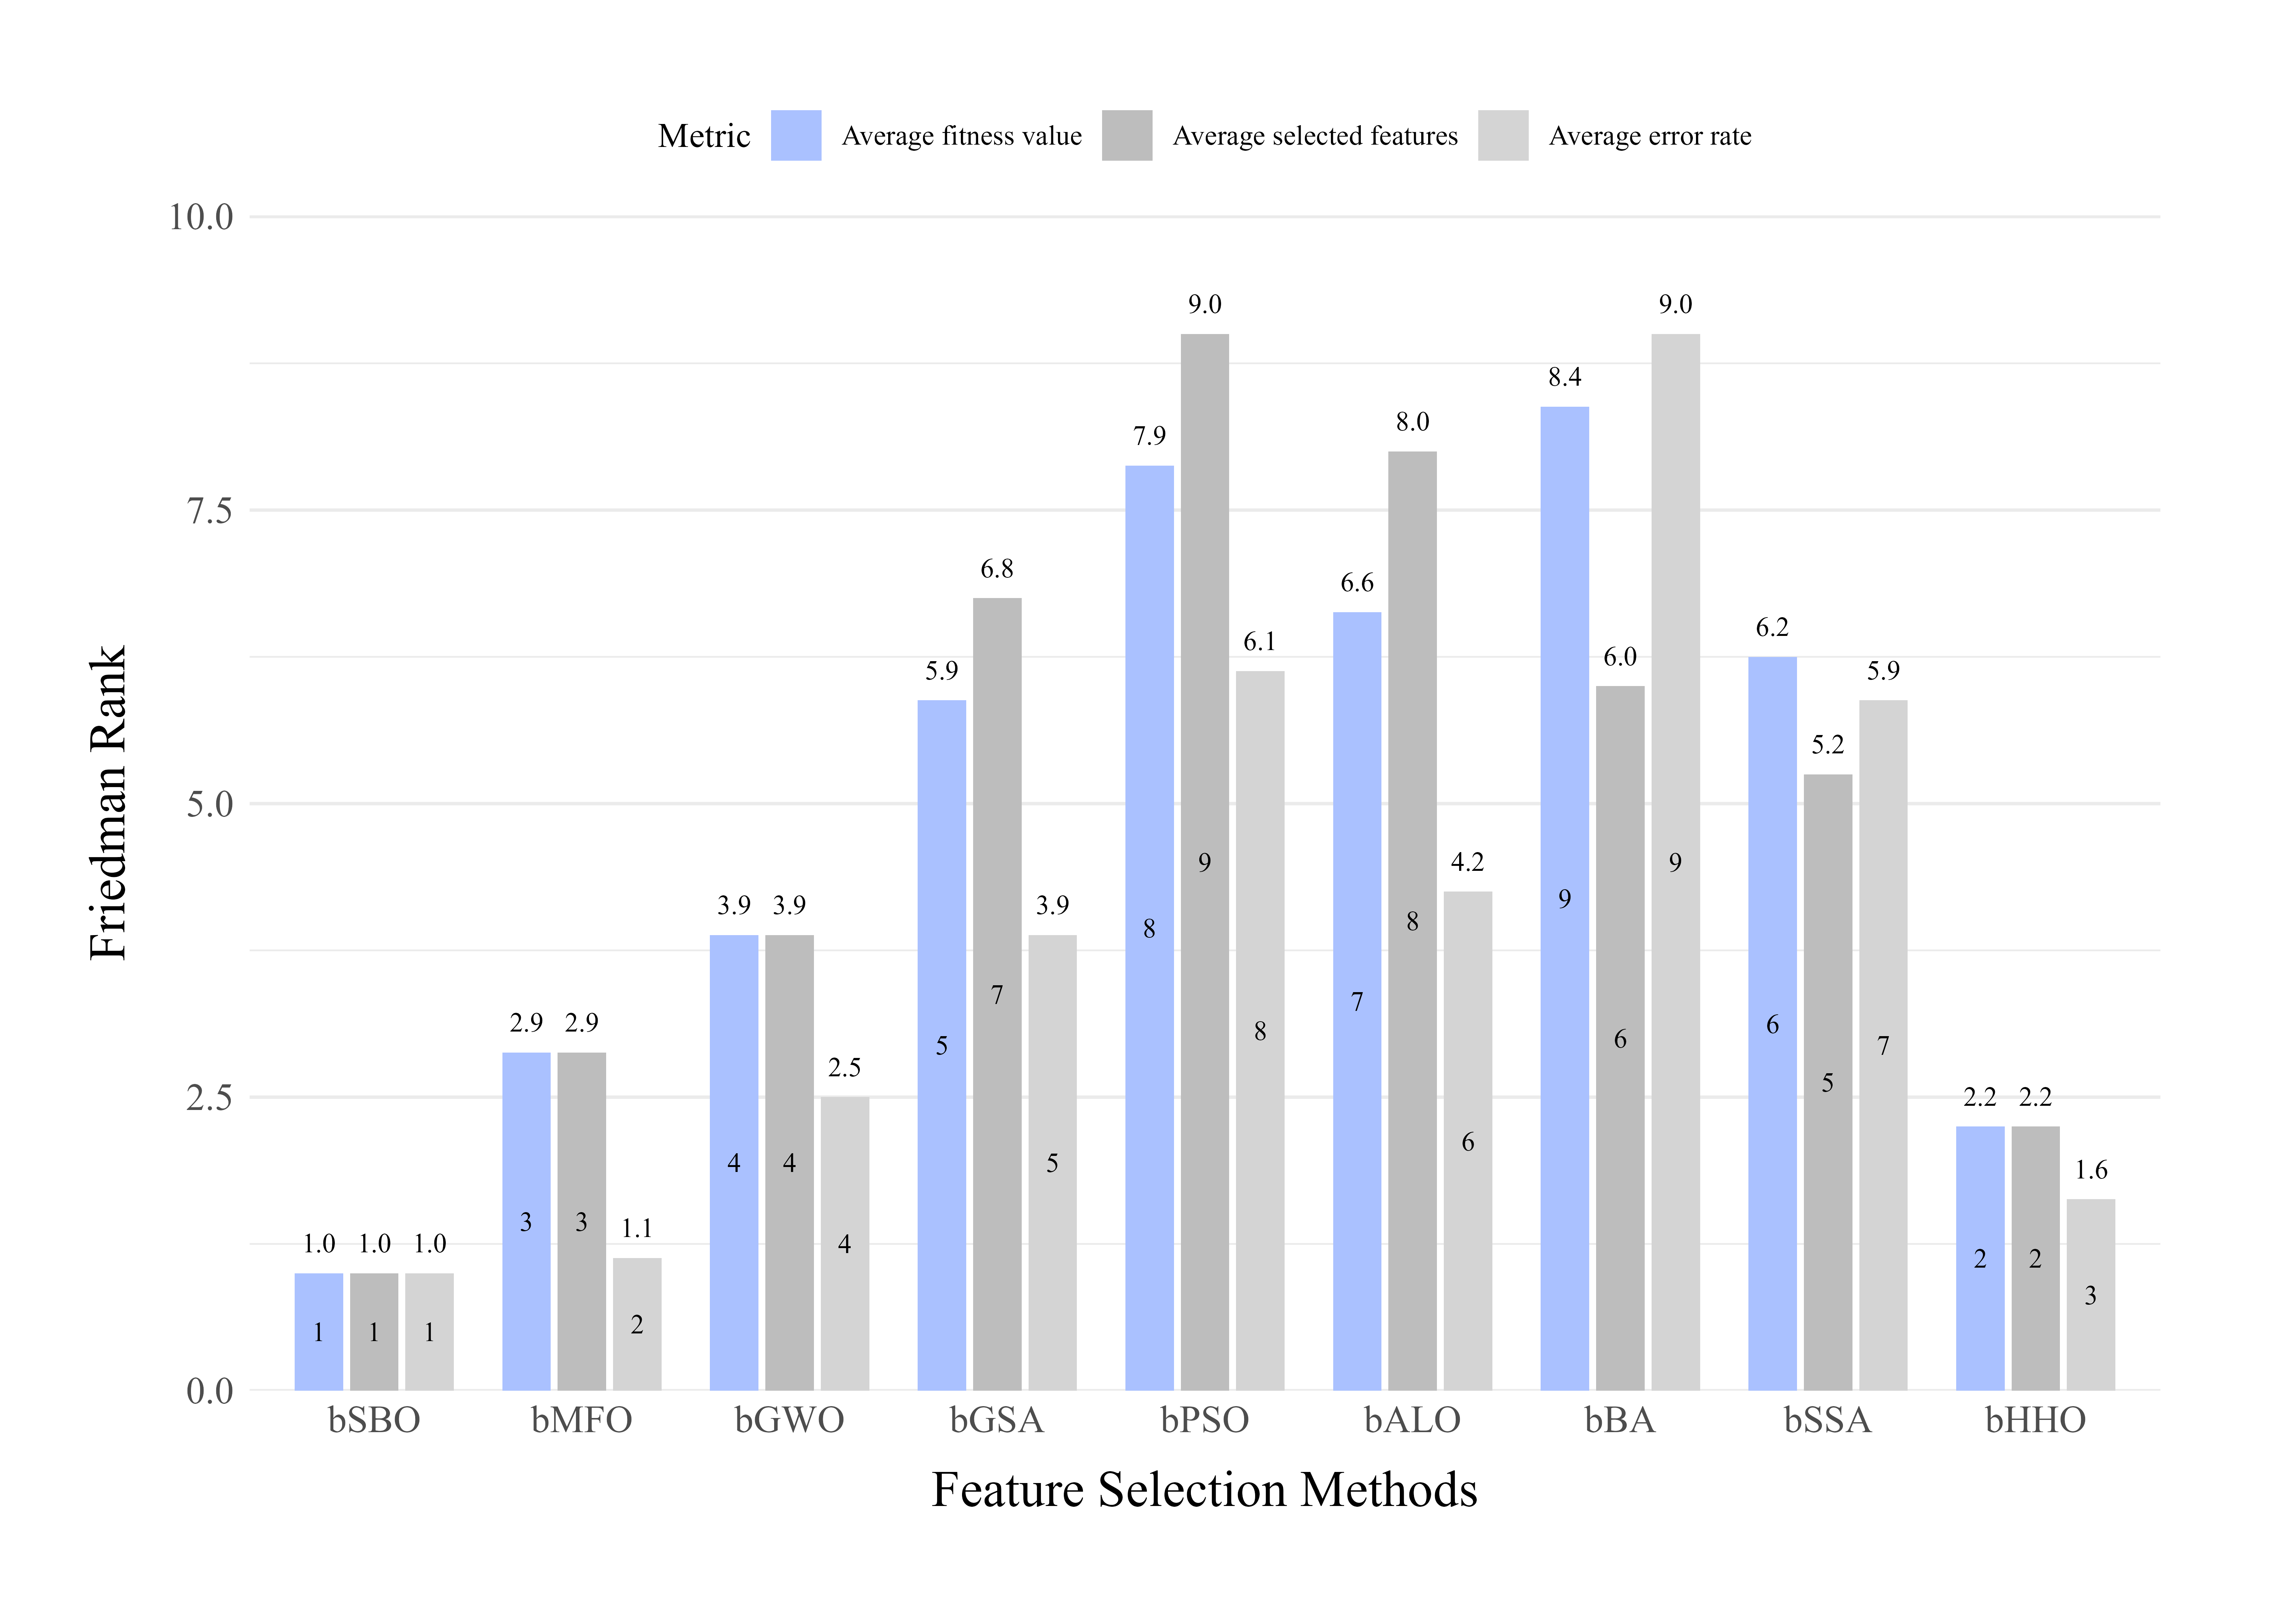
\includegraphics[width=\textwidth]{figures/chapter4/fig13_friedman_rank_feature_selection.png}
  \bicaption{三个指标的Friedman排名结果}{Friedman rank results over three metrics.}
  \label{fig:friedman_rank_feature_selection}
\end{figure}



相比之下，其他优化器表现出更大的排名波动，反映了在不同评估准则下的性能不一致性。值得注意的是，bSSA表现出显著的排名变异性，表明与bSBO相比缺乏鲁棒性。柱状图有效地说明了这些差异，从而突显了bSBO在所评估优化器中的稳定性和整体优越性能。

图14展示了每个优化器在多次迭代中的收敛曲线，显示了在每个数据集上向最优适应度值的进展。曲线表明bSBO在所有九个数据集上比其他优化器更快地达到最优适应度值，特别是在前50次迭代内。这表明虽然其他优化器可能经历早期停滞，但bSBO继续高效地识别更优的特征子集。具体而言，对于Prostate\_Tumor数据集，bHHO展示了相对于bSBO的竞争性能。更仔细的检查揭示了bSBO可能不太明显的微妙优势。

\begin{figure}[htbp]
  \centering
  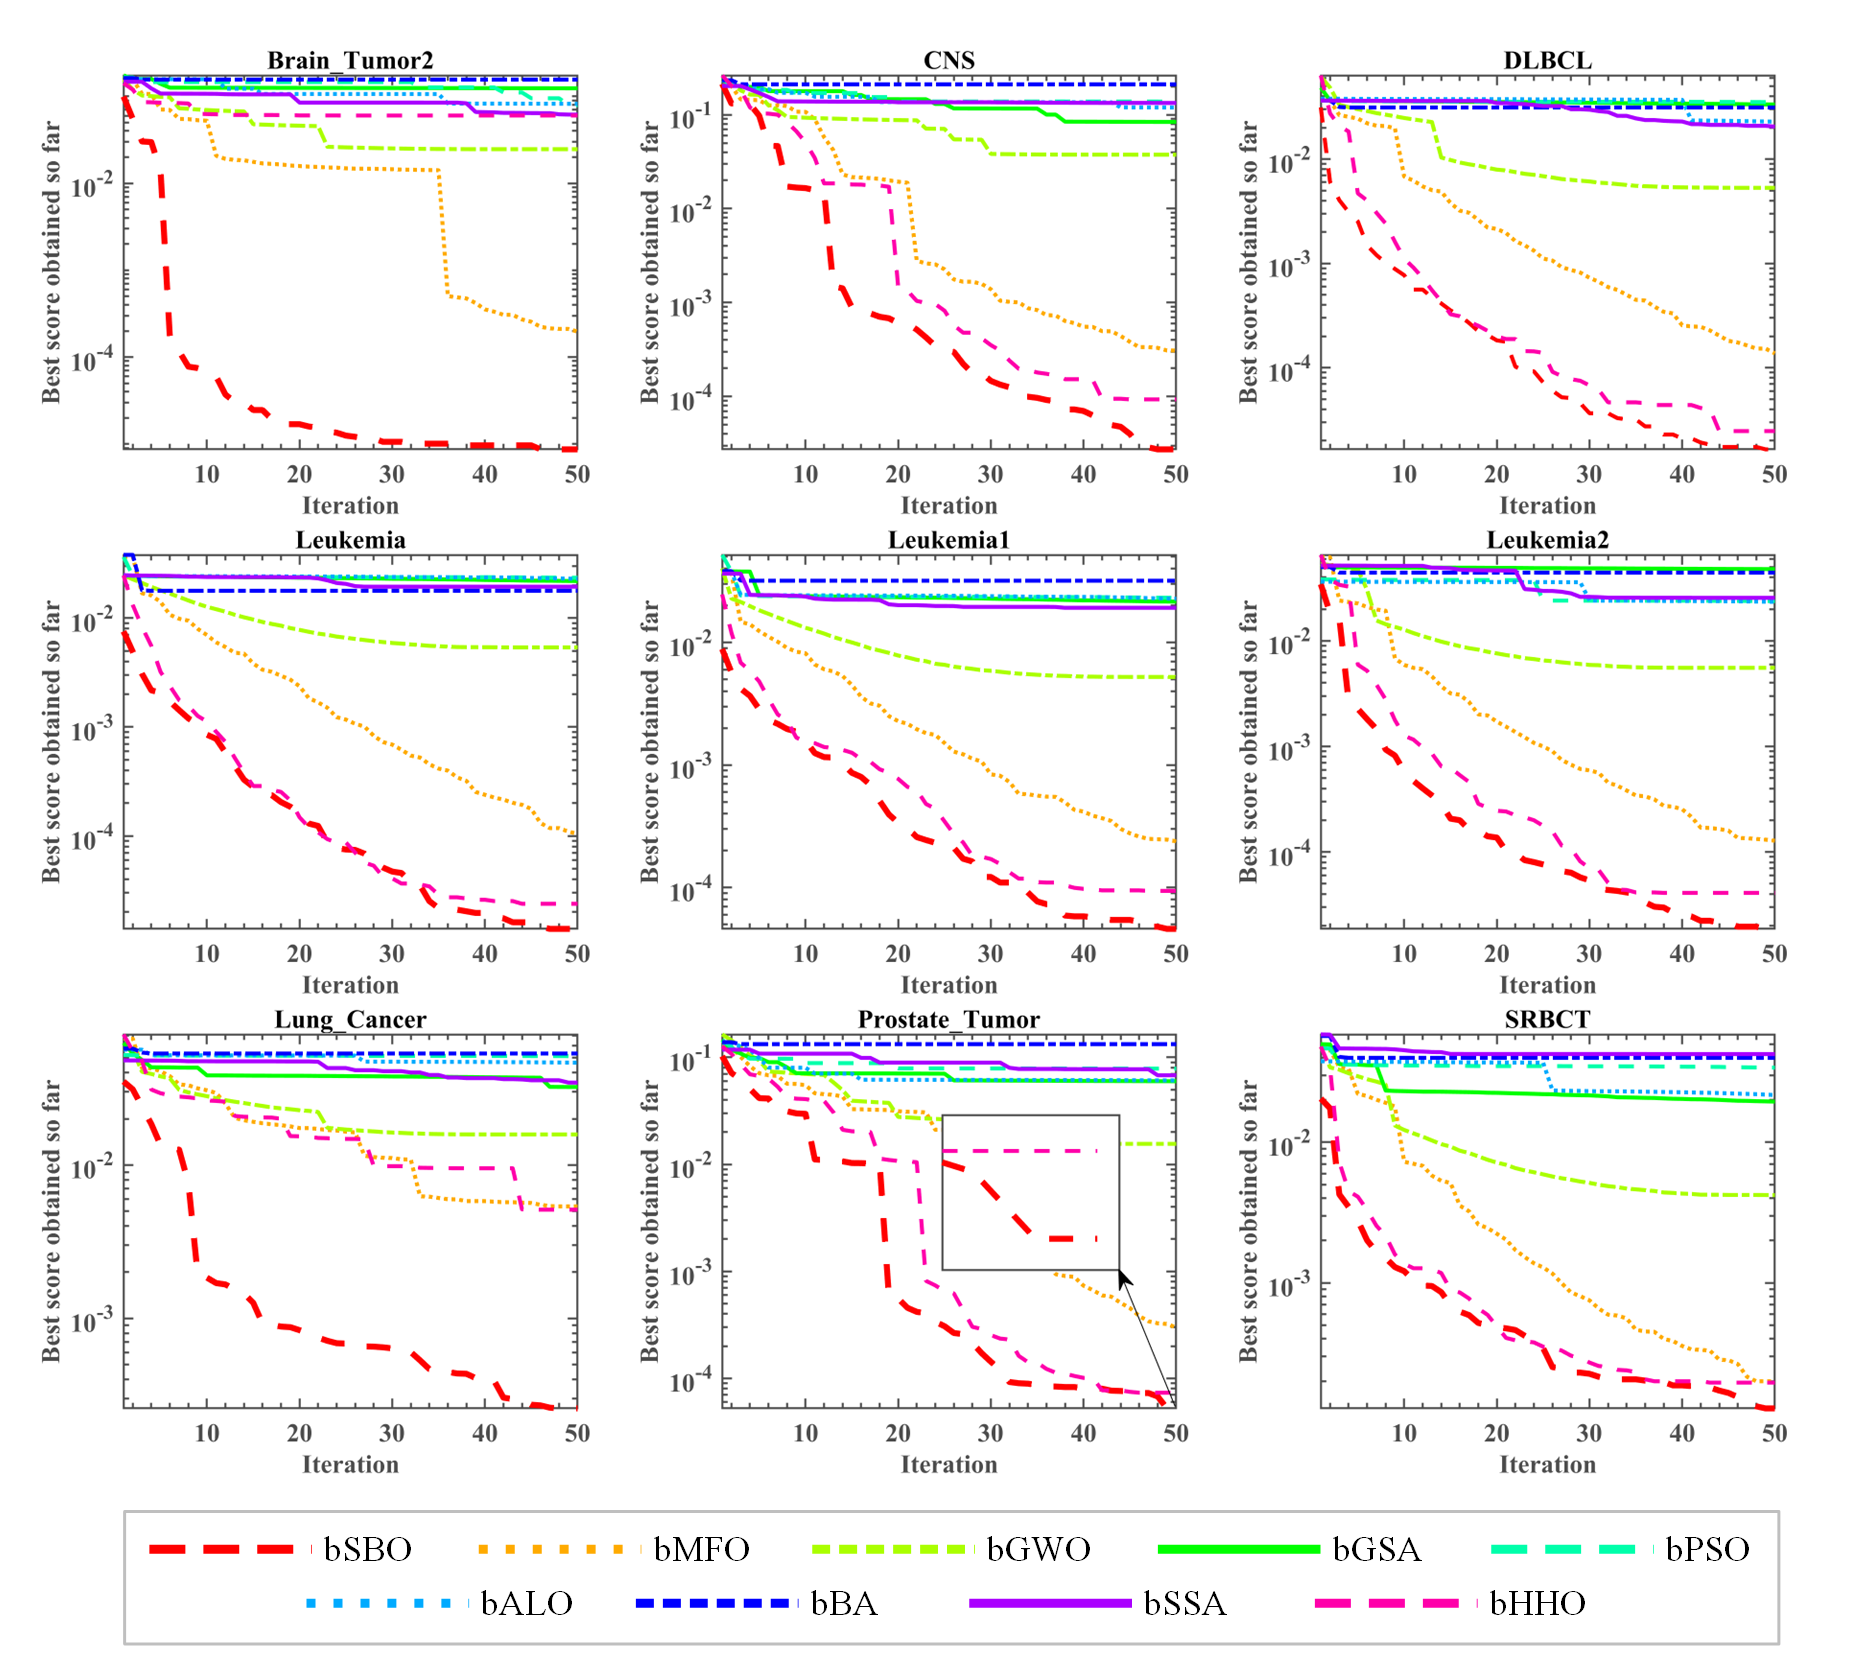
\includegraphics[width=\textwidth]{figures/chapter4/fig14_convergence_bSBO.png}
  \bicaption{bSBO与八种二值优化器在九个数据集上的收敛曲线}{Convergence curves of bSBO and eight binary optimizers over nine datasets.}
  \label{fig:convergence_bSBO}
\end{figure}



关于特征选择任务的实验结果有效地突显了bSBO卓越的优化能力，这得益于V型转换函数的支持，该函数巧妙地将SBO算法的能力从连续优化转换到离散优化场景。bSBO的性能通过三个不同的指标进行了全面评估，突显了其优越的优化能力。这些令人印象深刻的结果归因于SBO算法固有的全局优化强度。此外，人类社会向上流动的数学建模赋予了SBO独特的优势，反映了个体在复杂社会网络中与高地位同伴联系和学习的方式。通过获取和利用有价值的信息和资源，个体可以增强自己的能力——类似于SBO算法如何受益于其全面的全局搜索策略，向改进的解方向演化。SBO中这种类人的学习和改进动态证明了其设计的合理性，显著促进了其在特征选择任务中的有效性。

在此成功的基础上，下一节将bSBO的应用扩展到图像分割领域，利用其优化能力来解决多阈值分割挑战。


\subsection{多阈值图像分割}

多阈值图像分割是图像分析中的关键过程，涉及确定多个最优阈值以根据灰度变化将图像划分为不同区域\cite{sbo_ref79}。该技术不仅有助于将关键结构从背景中分离出来，还提高了复杂成像场景中的诊断准确性，例如乳腺癌检测。通过划分代表各种组织类型或病理区域的区域，多阈值分割在临床决策和治疗规划中发挥着关键作用。

多阈值分割方法主要可分为三类：基于直方图的方法、基于熵的方法和基于优化的方法——每种方法都有独特的阈值选择机制。基于直方图的方法通过分析像素灰度分布来获取候选阈值，从而利用图像数据中的自然聚类\cite{sbo_ref80}。相比之下，基于熵的技术，如使用Kapur熵或Tsallis熵的技术，旨在最大化分割区域的信息含量或同质性\cite{sbo_ref81}。与前两者不同，基于优化的方法将分割任务转化为搜索问题，其中适应度函数评估候选阈值集的质量\cite{sbo_ref82}。后一种方法通常使用MAs，它们善于在高维搜索空间中导航并避免局部最优，尽管代价是增加了计算复杂度。

本文特别关注使用Renyi熵作为适应度函数来搜索最优阈值集。通过将Renyi熵与鲁棒的搜索策略相集成，本文的方法有效地解决了图像噪声和灰度不均匀性等常见挑战，从而提高了分割精度和计算效率。后续各节详细介绍了实验设置，包括计算环境、参数配置和性能评估指标，随后将所提方法应用于乳腺癌图像的分割。通过这些实验，本文展示了所提技术在准确划分肿瘤区域方面的潜力，最终有助于改善诊断结果。


\subsubsection{实验设置}

所提SBO在多阈值图像分割中的性能在包含9张乳腺癌组织学图像的数据集上进行了评估。这些图像来源于IDC数据集\cite{sbo_ref83}，统一调整为224 $\mathrm{\times}$ 224像素。图像按A到I依次标记，如图15所示，同时展示了其对应的二维直方图，说明了阈值确定所需的灰度分布。

为评估SBO方法的广泛有效性和鲁棒性，使用三种不同的阈值配置进行了分割实验——具体为6、12和18个阈值。将所提SBO与7种先进的元启发式算法进行比较，分别是：Levy飞行结合反向学习的改进果蝇优化算法（LSEOFOA）\cite{sbo_ref84}、改进鲸鱼优化算法（IWOA）\cite{sbo_ref85}、改进灰狼优化器（IGWO）\cite{sbo_ref86}、自适应正弦余弦算法（ASCA）\cite{sbo_ref87}、迭代映射与局部逃逸增强的樽海鞘群算法（ILSSA）\cite{sbo_ref88}、有效Harris Hawks算法改进的樽海鞘群算法（EHSSA）\cite{sbo_ref89}以及基于生物地理学习的粒子群优化（BLPSO）\cite{sbo_ref90}。所有方法在相同的实验条件下进行测试。

对于每个分割任务，每种算法独立执行30次以减轻随机变异的影响。随后记录结果的平均值（Avg）和标准差（Std）。所有实验保持统一的种群大小20，每种算法在100次迭代后终止，以确保比较分析的公平性。此外，所有方法均使用其原始出版物中确定的默认参数值运行。

分割质量通过峰值信噪比（PSNR）、特征相似性指数（FSIM）和结构相似性指数（SSIM）进行定量评估。这些指标共同评估了分割图像相对于原始数据的保真度、特征保持和结构完整性。该全面的实验框架，凭借其受控的条件和标准化的评估准则，为比较SBO算法与其他基于MA方法的性能提供了鲁棒的基础。



\begin{figure}[htbp]
  \centering
  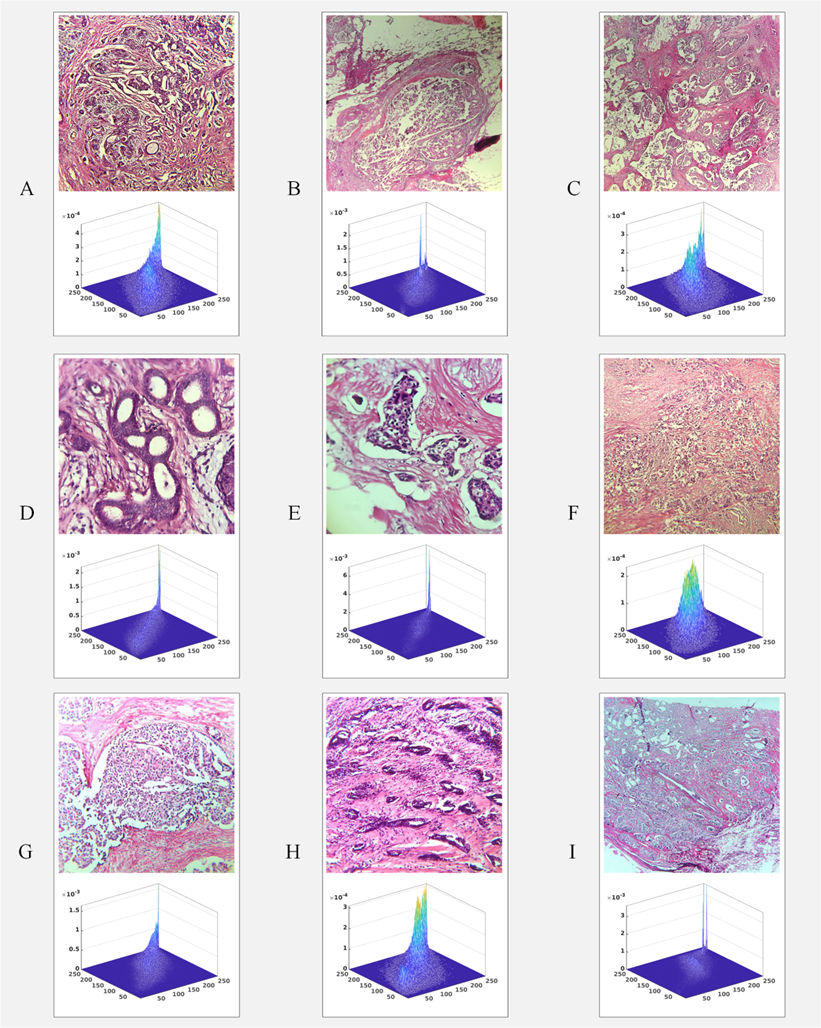
\includegraphics[width=\textwidth]{figures/chapter4/fig15_original_images_2D_histogram.png}
  \bicaption{原始图像及对应的二维直方图}{Original images and corresponding 2D-histogram.}
  \label{fig:original_images_2D_histogram}
\end{figure}




\subsubsection{实验结果与分析}

乳腺癌图像的分割过程通过系统化的多阶段流水线实现，如图16所示。整体过程详述如下。

首先，每张乳腺癌组织学图像被输入并调整为224 $\mathrm{\times}$ 224像素的固定尺寸，以确保数据集的一致性。这种标准化便于结果的一致处理和比较。随后，调整后的图像被转换为灰度格式，通过将图像简化为单通道来简化灰度分析，同时保留关键的结构信息。

同时，对灰度图像应用非局部均值（NLM）滤波技术。这一去噪步骤对于减轻噪声影响至关重要，从而提高图像数据质量以进行后续处理。NLM算法利用图像块中的冗余信息来实现有效的噪声降低，同时保留精细细节。

下一阶段涉及二维直方图的构建，这是多阈值分割方法中的关键组成部分。该直方图通过组合原始灰度图像与其对应的NLM滤波版本生成。由此得到的基于NLM的二维直方图封装了图像中固有的灰度信息和纹理特征，为阈值确定提供了更丰富的表示。

在直方图构建之后，启动阈值选择过程。使用MAs搜索最大化所选适应度函数（具体为Renyi熵）的最优阈值。该优化过程系统性地探索解空间，基于组合的灰度和纹理线索识别最佳划分图像的阈值集。

一旦确定了最优阈值，将其应用于原始图像的分割。该分割过程将图像划分为对应不同灰度水平的不同区域，有效地勾勒出感兴趣的区域。然后对分割图像进行后处理以生成Jet色图表示，这在视觉上增强了边界的划定，有助于对分割结果进行更直观的解读。



\begin{figure}[htbp]
  \centering
  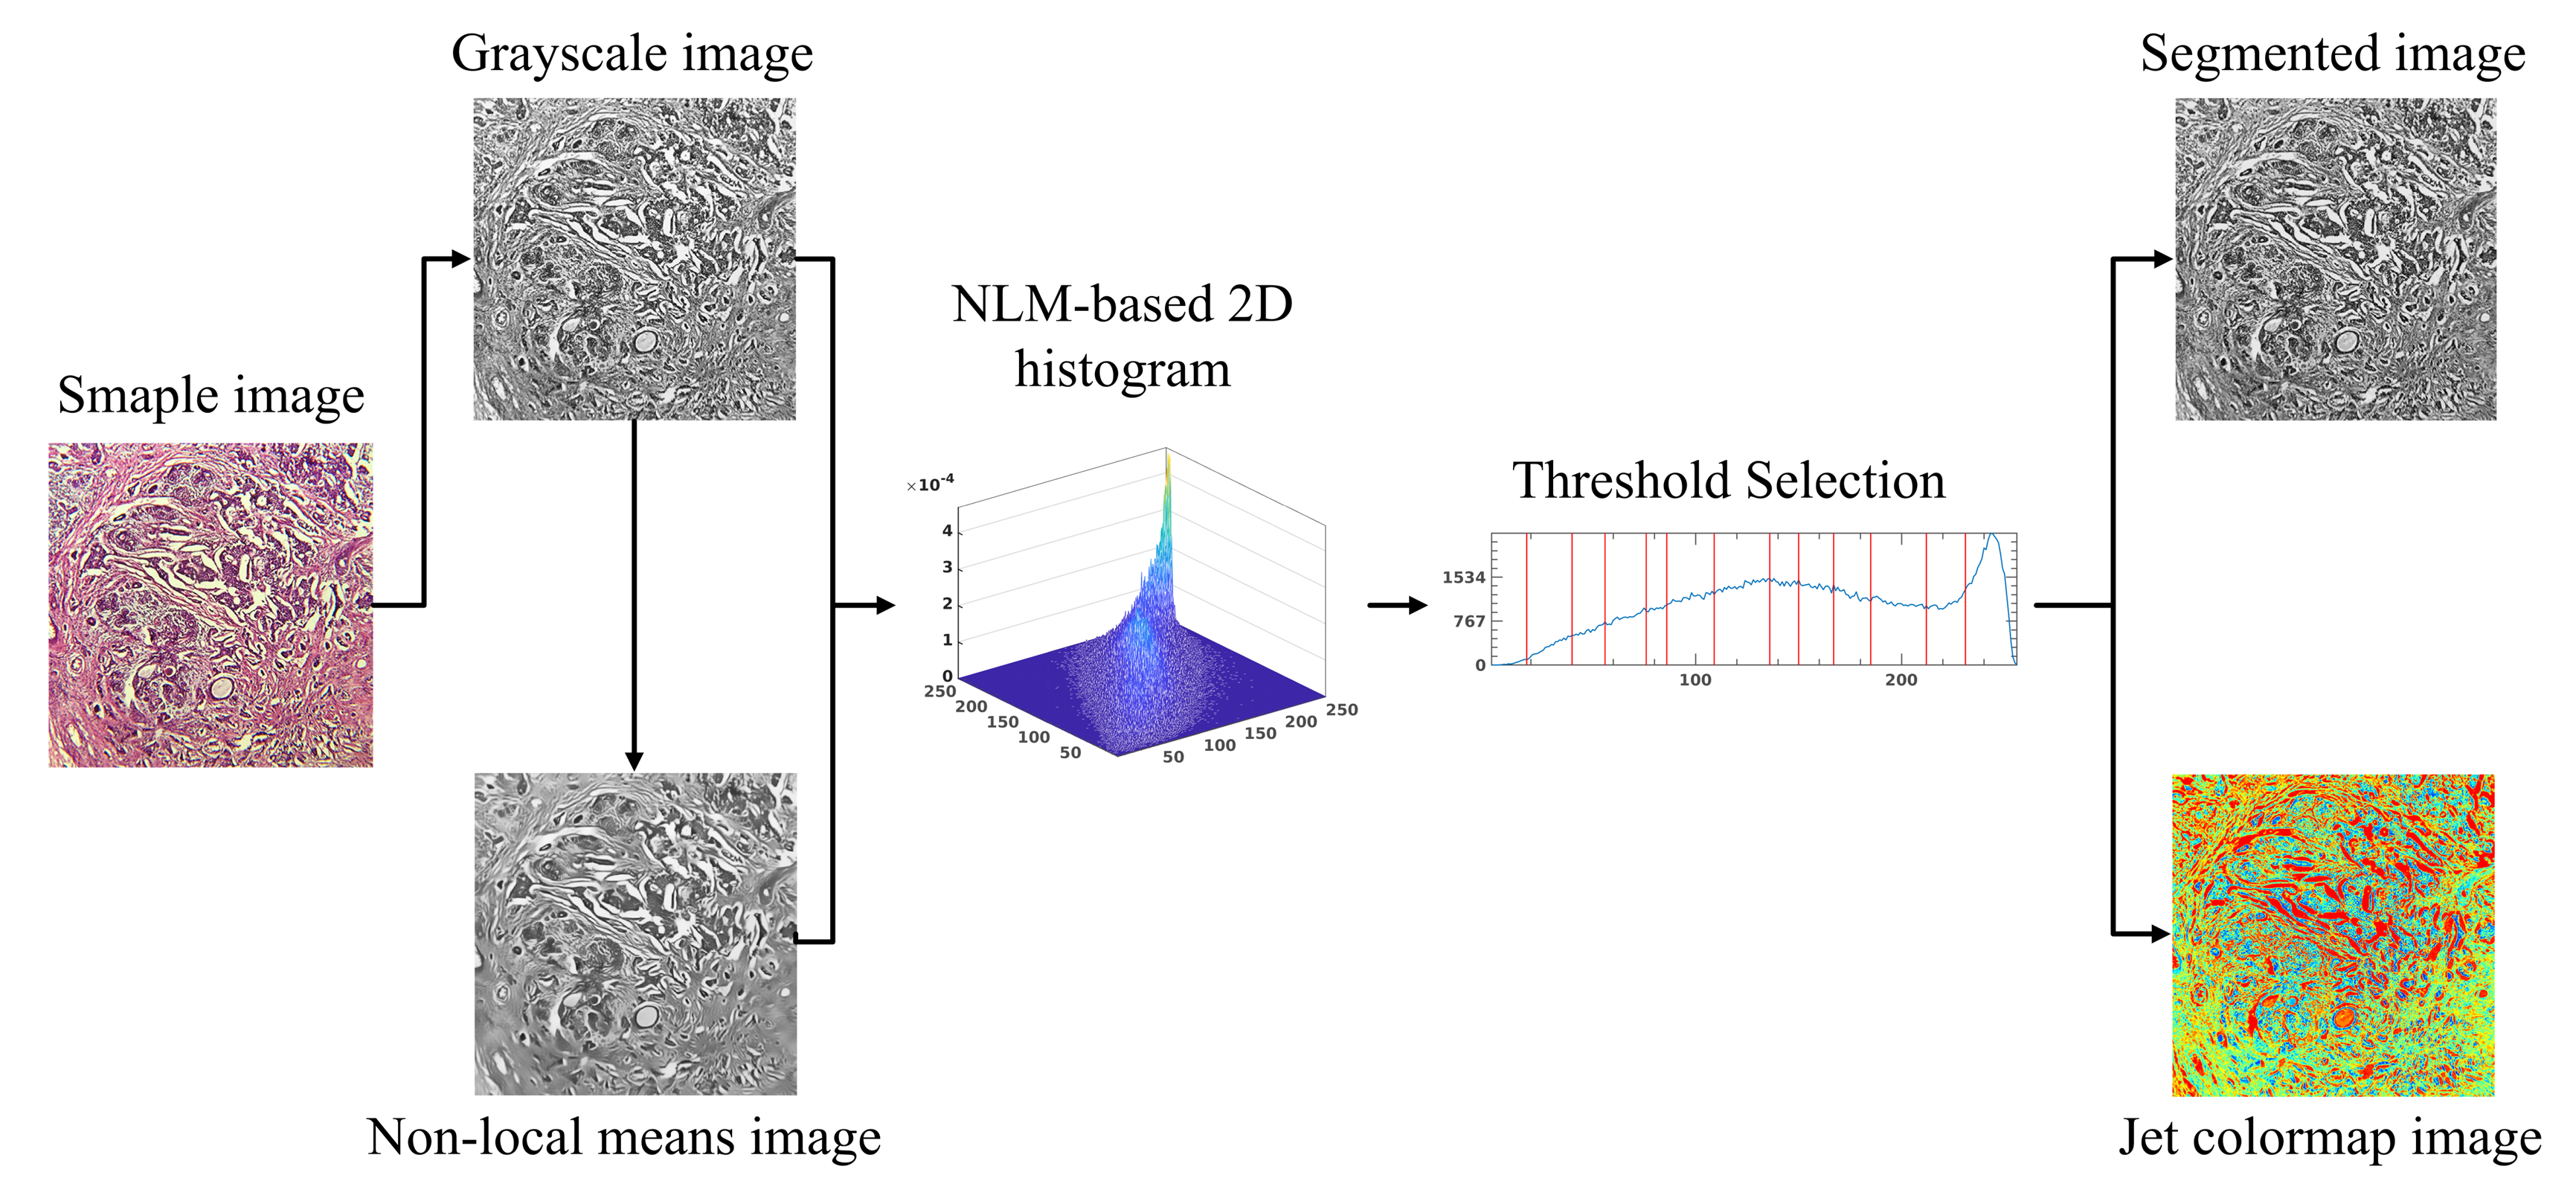
\includegraphics[width=\textwidth]{figures/chapter4/fig16_flowchart_image_segmentation.png}
  \bicaption{多阈值图像分割流程图}{Flowchart of multi-threshold image segmentation.}
  \label{fig:flowchart_image_segmentation}
\end{figure}



按照上述分割流水线，本节展示了实验结果、分析和可视化。

所提基于SBO模型的性能使用三个广泛采用的指标进行评估：PSNR、FSIM和SSIM。使用6、12和18个阈值水平的分割任务结果分别全面总结在表A. 9\textbf{至}表A. 11中。对每种阈值配置进行了30次独立运行的指标计算，并报告了平均值和标准差。这些表格以粗体突出显示最优性能值，便于直观识别最佳结果。

使用6个阈值的分割任务性能指标在图17中进一步可视化，以热力图的形式展示PSNR、FSIM和SSIM分数。在热力图中，较暖的颜色对应较高的指标值，表示更优的分割质量，而较冷的颜色表示较低的分数。对这些可视化的详细分析表明，在所有三个指标上，所提基于SBO的方法与其他评估方法相比始终获得最高分数。



\begin{figure}[htbp]
  \centering
  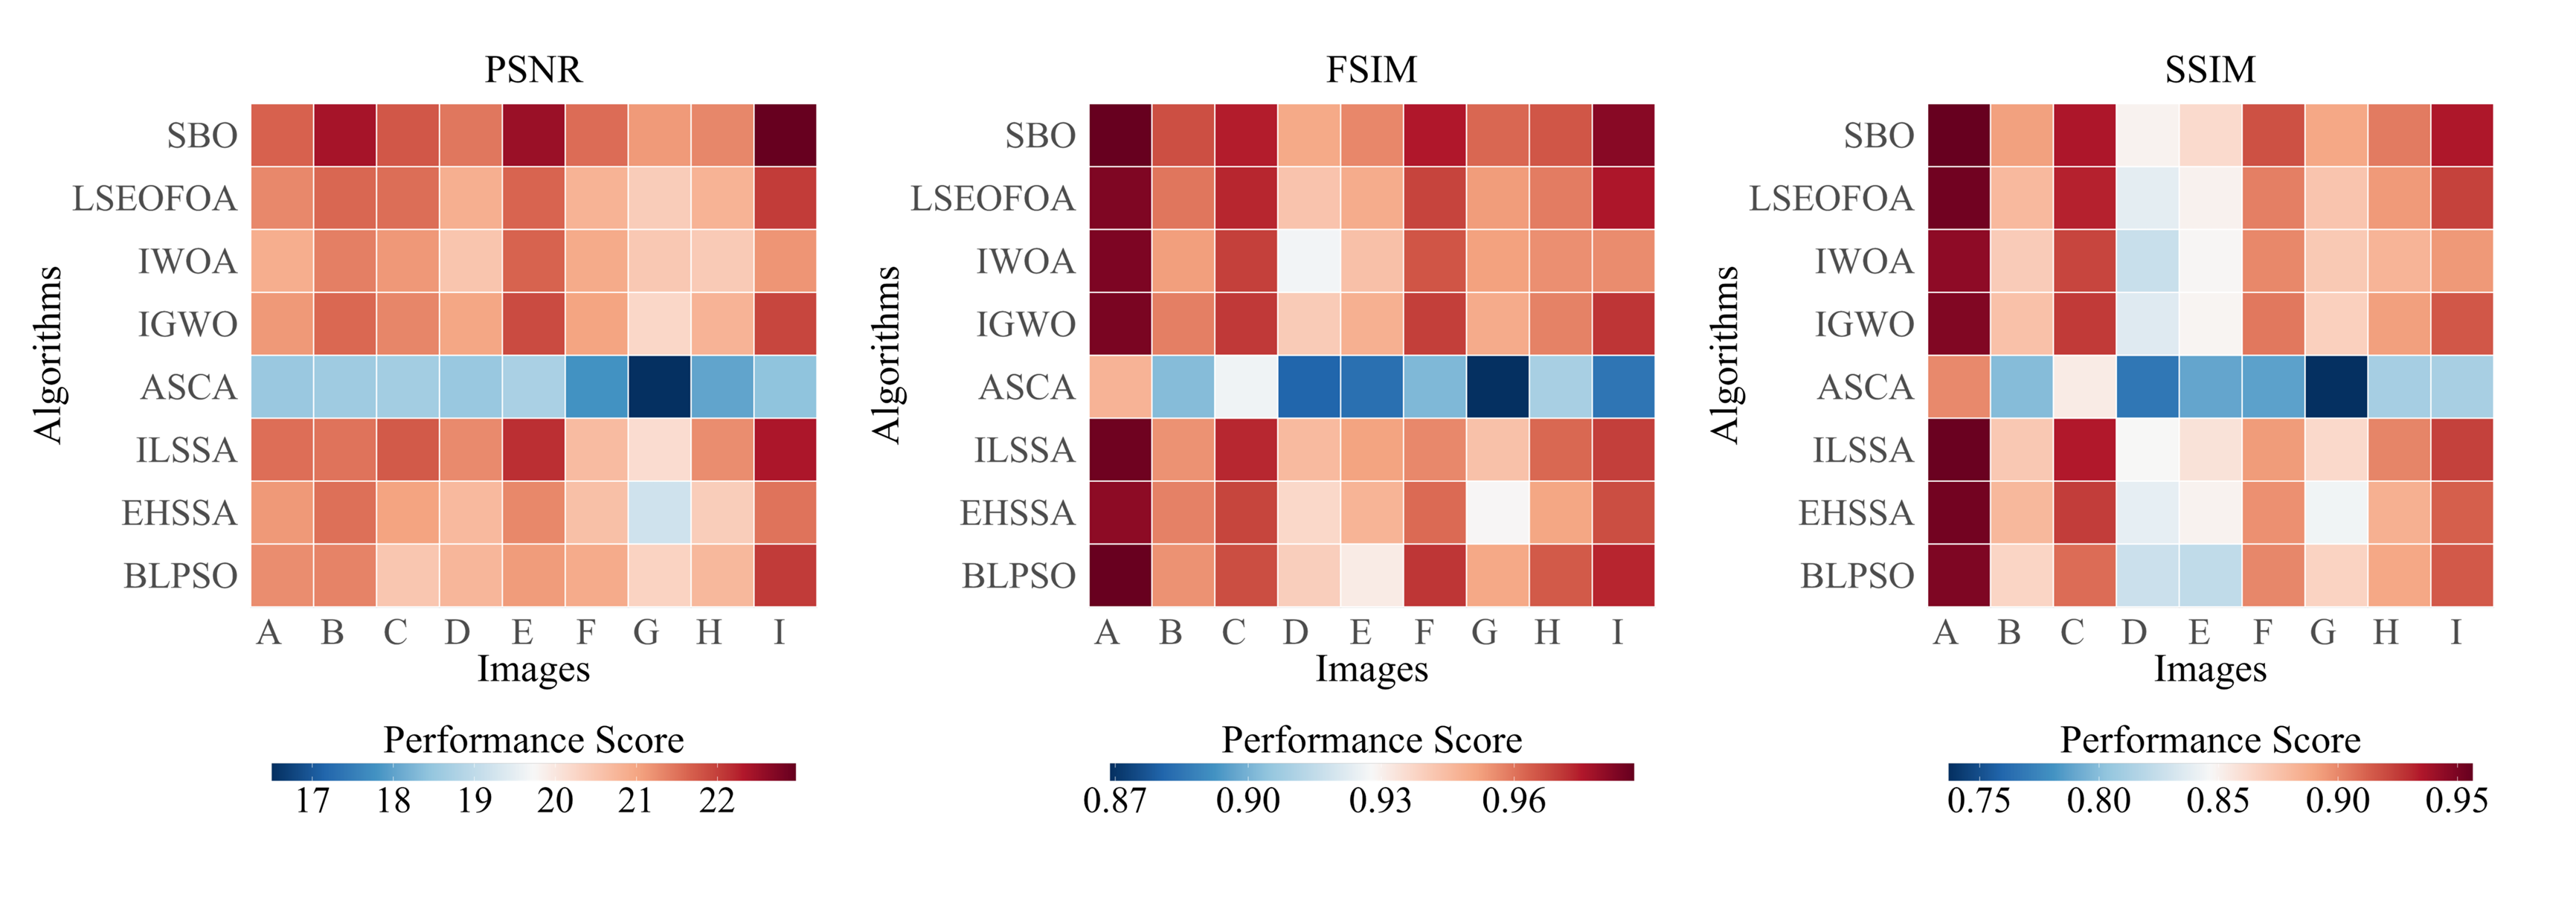
\includegraphics[width=\textwidth]{figures/chapter4/fig17_heatmap_PSNR_FSIM_SSIM.png}
  \bicaption{6个阈值水平下PSNR、FSIM和SSIM结果的热力图}{Heatmap for PSNR, FSIM, and SSIM result over 6 threshold level.}
  \label{fig:heatmap_PSNR_FSIM_SSIM}
\end{figure}



在使用12个阈值进行的实验中，图18展示了迭代优化过程中Renyi熵值的收敛曲线。虽然基于SBO的方法在早期迭代中最初表现出较低的熵值，但它稳步改善并最终在最后一次迭代（第100次迭代）时收敛到最优阈值配置。这种收敛行为突显了算法克服初始次优性并有效探索解空间以识别最佳阈值的能力。

\begin{figure}[htbp]
  \centering
  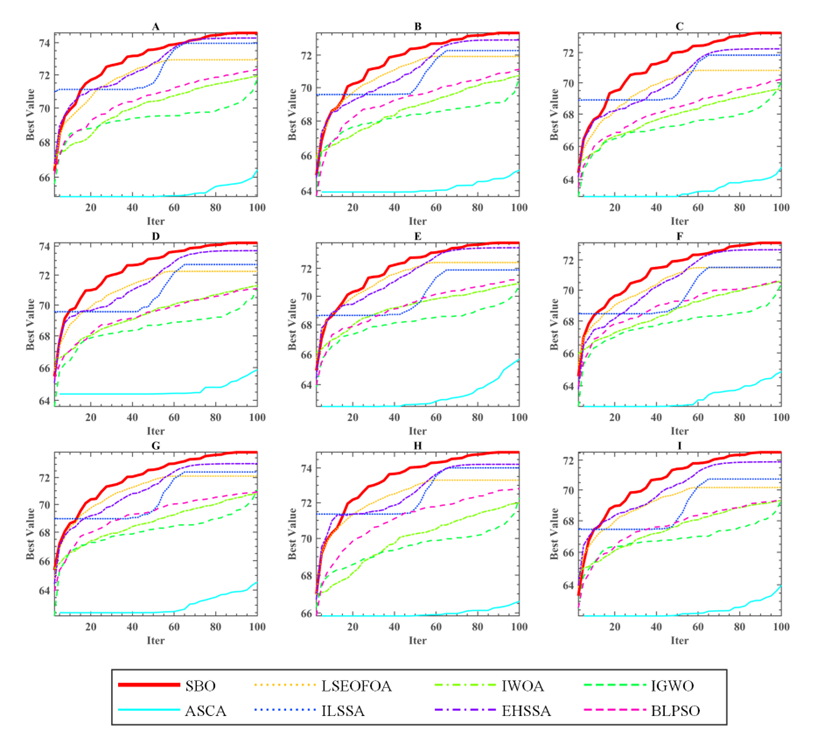
\includegraphics[width=\textwidth]{figures/chapter4/fig18_convergence_entropy.png}
  \bicaption{12个阈值水平下熵值的收敛曲线}{Convergence curves of the entropy value by 12 threshold level.}
  \label{fig:convergence_entropy}
\end{figure}



对于涉及18个阈值的分割任务，图19比较了图像B的Jet色图分割结果与其对应的原始图像。Jet色图通过为相似灰度区域分配不同颜色来增强视觉解读。比较分析表明，基于SBO的方法识别出更优的阈值，产生了灰度相近区域被更准确地归类在一起的分割图像。

\begin{figure}[htbp]
  \centering
  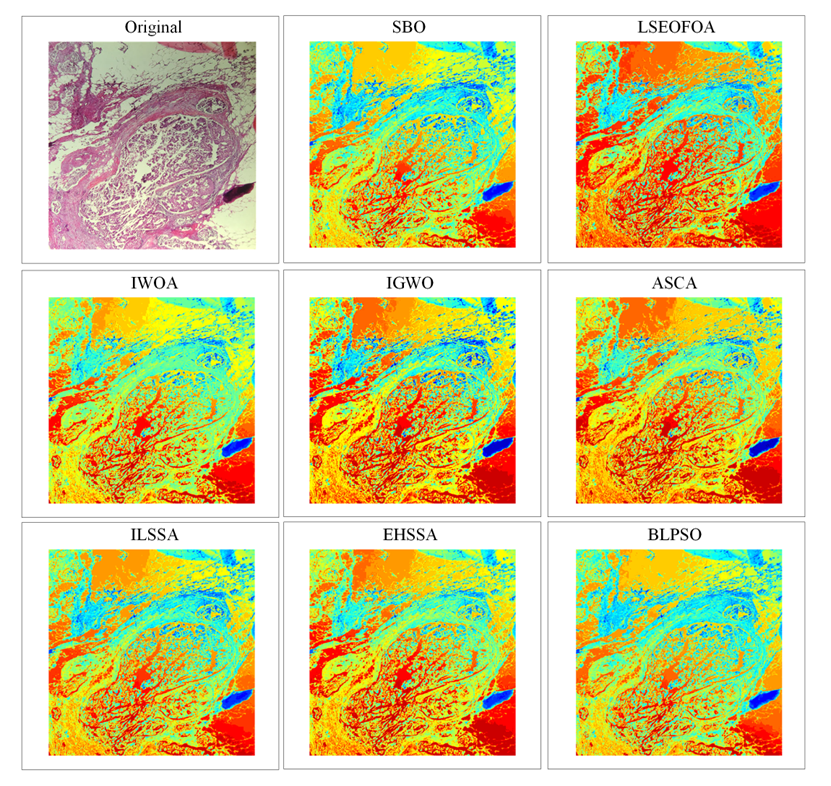
\includegraphics[width=\textwidth]{figures/chapter4/fig19_jet_colormap_segmentation.png}
  \bicaption{图像B在18个阈值水平下的Jet色图分割结果}{Jet colormap segmentation result of image B over 18 threshold level.}
  \label{fig:jet_colormap_segmentation}
\end{figure}



总体而言，实验结果和配套可视化提供了所提基于SBO方法优越性的有力证据。在各种阈值水平和评估指标下，该方法获得了更高的定量分数并产生了视觉上连贯的分割结果，从而证实了其在临床诊断应用中的潜在实用性。


\section{本章小结}

本文提出了SBO，一种受人类地位驱动社会行为启发的MA，其中个体通过战略性建立联系和资源交换寻求进步。SBO将这种动态转化为计算模型，平衡探索和开发以高效导航复杂的优化空间。在探索阶段，代理在由自身位置、最成功同伴和高地位个体定义的高地位圈子内移动，确保多样化且有效的搜索。开发通过局部精炼实现，增强解的质量，确保向最优解收敛。

SBO的有效性通过IEEE CEC 2017测试套件的基准函数得到验证，在10、30、50和100维度上优于13种最先进的元启发式算法，包括人类行为启发算法、最新方法以及经典的PSO和DE变体。Wilcoxon符号秩检验和Friedman检验等统计分析证实了其优越的全局优化能力和可扩展性。此外，开发了二值变体bSBO用于特征选择，利用V型转换函数选择最少但最相关的特征子集。在9个高维UCI数据集上与8种二值优化器进行测试，bSBO始终展示了最优适应度，在保持高分类精度的同时选择了最少的特征。SBO还被应用于3个阈值水平的多阈值图像分割，在IDC数据集的9张乳腺癌组织学图像上与7种先进元启发式方法进行比较，有效识别了最优分割阈值，突显了其在现实世界应用中的通用性。

尽管SBO表现强劲，根据"没有免费午餐"定理\cite{sbo_ref95}，没有任何算法能在所有场景中都表现出色。未来的研究应探索SBO对多目标优化的适应、大规模问题的可扩展性以及与其他计算框架的混合化，以增强其鲁棒性和适用性。在更多领域的进一步测试将为其优化潜力提供更深入的见解，并有助于推动启发式优化方法的发展。

此外，动态多目标优化领域的最新进展，如具有多策略自适应选择的非归纳迁移学习方法\cite{sbo_ref91}和用于目标知识转移的级联模糊系统\cite{sbo_ref92}，为进一步增强提供了有价值的启示。这些方法解决了动态环境中的负迁移和刚性标注等挑战，可能启发SBO的未来扩展以有效处理时变优化问题。在未来的工作中，本文计划研究将此类先进技术集成到SBO中，旨在进一步提高其在动态环境中的适应性和性能。



% --- 附录：补充数据表格 ---
\section{附录：补充数据}

 见表A. 1-A. 11。

\begin{tabular}{|p{0.3in}|p{0.3in}|p{0.3in}|p{0.3in}|p{0.3in}|p{0.3in}|p{0.3in}|p{0.3in}|p{0.3in}|p{0.3in}|p{0.3in}|p{0.3in}|p{0.3in}|p{0.3in}|p{0.3in}|p{0.5in}|} \hline 
\multicolumn{16}{|p{4.8in}|}{\textbf{Table A. }1\textbf{. }Comparative results of SBO and state-of-the-art algorithms for 10-dimensional problems.\textbf{}} \\ \hline 
Fun & Item & SBO & TLBO & PO & HHO & RIME & ALCPSO & CLPSO & CGPSO & MSPSO & CMAES & DECLS & LSHADE\_cnEpSin & SCADE & SHADE \\ \hline 
F1 & Avg & 1.0000E+02 & 2.3180E+09 & 5.7825E+07 & 2.7350E+05 & 1.1951E+03 & 8.5399E+02 & 1.0876E+02 & 5.4781E+06 & 4.7180E+02 & \textbf{1.0000E+02} & 4.4133E+02 & \textbf{1.0000E+02} & 9.4471E+08 & \textbf{1.0000E+02} \\ \hline 
 & Std & 3.7899E-11 & 1.9307E+09 & 1.7239E+08 & 1.2752E+05 & 8.7649E+02 & 6.8933E+02 & 1.2166E+01 & 1.4214E+06 & 4.8450E+02 & \textbf{0.0000E+00} & 3.6559E+02 & 2.0441E-14 & 3.7498E+08 & \textbf{0.0000E+00} \\ \hline 
F2 & Avg & \textbf{3.0000E+02} & 5.6759E+03 & 3.0009E+02 & 3.0148E+02 & 3.0000E+02 & 3.6480E+02 & 3.0284E+02 & 3.2021E+02 & 3.0000E+02 & \textbf{3.0000E+02} & 9.5474E+02 & \textbf{3.0000E+02} & 3.4003E+03 & \textbf{3.0000E+02} \\ \hline 
 & Std & 4.4783E-14 & 3.5880E+03 & 4.5599E-01 & 8.6163E-01 & 2.7309E-03 & 2.1593E+02 & 2.1596E+00 & 6.3013E+00 & 4.4408E-08 & \textbf{0.0000E+00} & 4.1849E+02 & 3.5009E-14 & 1.1183E+03 & \textbf{0.0000E+00} \\ \hline 
F3 & Avg & 4.1681E+02 & 6.8320E+02 & 4.3204E+02 & 4.2885E+02 & 4.2373E+02 & 4.1831E+02 & 4.0063E+02 & 4.0779E+02 & \textbf{4.0000E+02} & 4.3130E+02 & 4.1887E+02 & 4.2302E+02 & 4.8082E+02 & 4.2927E+02 \\ \hline 
 & Std & 1.7155E+01 & 3.9742E+02 & 2.4709E+01 & 1.6903E+01 & 2.0094E+01 & 1.8927E+01 & 7.2505E-01 & 2.1031E+00 & \textbf{4.0814E-12} & 1.0612E+01 & 1.2199E+01 & 1.2929E+01 & 1.5995E+01 & 1.2557E+01 \\ \hline 
F4 & Avg & 5.2103E+02 & 5.3686E+02 & 5.4090E+02 & 5.3752E+02 & 5.1081E+02 & 5.1535E+02 & 5.0523E+02 & 5.3135E+02 & 5.2759E+02 & 6.9599E+02 & 5.0828E+02 & \textbf{5.0408E+02} & 5.4742E+02 & 5.0484E+02 \\ \hline 
 & Std & 1.0955E+01 & 1.2216E+01 & 2.2018E+01 & 1.5707E+01 & 3.7660E+00 & 7.0510E+00 & \textbf{1.3200E+00} & 1.3347E+01 & 8.2334E+00 & 1.1764E+02 & 1.4219E+00 & 1.8906E+00 & 6.1203E+00 & 1.8427E+00 \\ \hline 
F5 & Avg & 6.0000E+02 & 6.2154E+02 & 6.0194E+02 & 6.3246E+02 & 6.0002E+02 & 6.0000E+02 & \textbf{6.0000E+02} & 6.0495E+02 & 6.0932E+02 & 6.8167E+02 & \textbf{6.0000E+02} & 6.0000E+02 & 6.1657E+02 & 6.0000E+02 \\ \hline 
 & Std & 4.8843E-03 & 6.4558E+00 & 7.1750E+00 & 7.7477E+00 & 7.9383E-03 & 5.4205E-03 & 6.6759E-14 & 4.6937E+00 & 1.0207E+01 & 1.8514E+01 & \textbf{3.6566E-14} & 2.8894E-04 & 3.2689E+00 & 1.8204E-05 \\ \hline 
F6 & Avg & 7.2736E+02 & 7.9128E+02 & 7.2114E+02 & 8.0159E+02 & 7.2062E+02 & 7.2288E+02 & 7.1630E+02 & 7.3992E+02 & 7.2248E+02 & 1.5829E+03 & 7.1971E+02 & \textbf{7.1338E+02} & 7.8912E+02 & 7.1427E+02 \\ \hline 
 & Std & 7.2747E+00 & 3.5415E+01 & 6.5920E+00 & 3.1667E+01 & 4.9622E+00 & 4.9199E+00 & \textbf{1.3102E+00} & 6.1315E+00 & 5.0845E+00 & 4.1952E+02 & 2.1805E+00 & 1.5493E+00 & 1.3146E+01 & 2.3054E+00 \\ \hline 
F7 & Avg & 8.2225E+02 & 8.3788E+02 & 8.2739E+02 & 8.4522E+02 & 8.1232E+02 & 8.1242E+02 & 8.0513E+02 & 8.3708E+02 & 8.2987E+02 & 9.8467E+02 & 8.0861E+02 & \textbf{8.0441E+02} & 8.5401E+02 & 8.0444E+02 \\ \hline 
 & Std & 9.2619E+00 & 1.1309E+01 & 1.5845E+01 & 1.3262E+01 & 4.6139E+00 & 4.5775E+00 & \textbf{1.1352E+00} & 1.0167E+01 & 8.3229E+00 & 7.1960E+01 & 1.7763E+00 & 1.5596E+00 & 9.0722E+00 & 1.3255E+00 \\ \hline 
F8 & Avg & 9.0158E+02 & 1.1883E+03 & 1.8315E+03 & 1.7995E+03 & 9.0004E+02 & 9.0045E+02 & 9.0000E+02 & 9.5939E+02 & 1.1690E+03 & 4.7794E+03 & \textbf{9.0000E+02} & 9.0013E+02 & 1.1973E+03 & 9.0007E+02 \\ \hline 
 & Std & 3.0779E+00 & 1.8033E+02 & 1.4153E+02 & 2.9037E+02 & 1.1647E-01 & 6.6575E-01 & 4.3803E-07 & 1.8652E+02 & 2.5310E+02 & 1.3525E+03 & \textbf{0.0000E+00} & 2.7253E-01 & 1.3439E+02 & 1.5588E-01 \\ \hline 
F9 & Avg & 1.3851E+03 & 1.9715E+03 & 1.6257E+03 & 1.8197E+03 & 1.2828E+03 & 1.4065E+03 & 1.1400E+03 & 1.9250E+03 & 1.5005E+03 & 2.6178E+03 & 1.3735E+03 & \textbf{1.0878E+03} & 2.3300E+03 & 1.1061E+03 \\ \hline 
 & Std & 2.6189E+02 & 2.6708E+02 & 1.8066E+02 & 3.0548E+02 & 1.9557E+02 & 2.8974E+02 & \textbf{6.3268E+01} & 2.2613E+02 & 1.6301E+02 & 4.6360E+02 & 1.2582E+02 & 7.2997E+01 & 1.5129E+02 & 8.9242E+01 \\ \hline 
F10 & Avg & 1.1083E+03 & 1.1963E+03 & 1.8307E+03 & 1.1314E+03 & 1.1079E+03 & 1.1123E+03 & 1.1025E+03 & 1.1175E+03 & 1.1127E+03 & 1.1263E+03 & 1.1032E+03 & 1.1071E+03 & 1.2089E+03 & \textbf{1.1018E+03} \\ \hline 
 & Std & 4.2547E+00 & 9.5005E+01 & 2.9738E+03 & 2.0663E+01 & 4.2869E+00 & 1.2376E+01 & 1.0394E+00 & 7.7493E+00 & 7.3783E+00 & 1.5009E+01 & \textbf{1.0077E+00} & 8.0343E+00 & 3.7841E+01 & 1.2827E+00 \\ \hline 
F11 & Avg & 2.0189E+03 & 1.1538E+06 & 4.0045E+05 & 4.1113E+06 & 1.8147E+04 & 2.1672E+04 & 1.8209E+04 & 1.2964E+06 & 2.6195E+03 & 1.6768E+03 & 7.1923E+04 & 1.6599E+03 & 1.4365E+07 & \textbf{1.4866E+03} \\ \hline 
 & Std & 1.2392E+03 & 2.2445E+06 & 9.0075E+05 & 5.2074E+06 & 1.3042E+04 & 1.3461E+04 & 1.7372E+04 & 1.5018E+06 & 2.8892E+03 & 1.9643E+02 & 4.2183E+04 & 2.3576E+02 & 9.1844E+06 & \textbf{1.6495E+02} \\ \hline 
F12 & Avg & 1.3090E+03 & 2.9516E+03 & 1.4632E+04 & 1.7880E+04 & 3.5650E+03 & 3.9140E+03 & 1.3348E+03 & 9.5724E+03 & 1.3683E+03 & 1.4794E+03 & 2.1266E+03 & 1.3679E+03 & 2.9126E+04 & \textbf{1.3048E+03} \\ \hline 
 & Std & 4.9077E+00 & 2.3298E+03 & 1.2823E+04 & 2.1559E+04 & 2.5377E+03 & 2.0317E+03 & 2.7892E+01 & 6.1609E+03 & 4.4587E+01 & 1.0798E+02 & 1.1207E+03 & 1.0372E+02 & 2.0590E+04 & \textbf{2.2110E+00} \\ \hline 
F13 & Avg & 1.4263E+03 & 1.4850E+03 & 3.1339E+03 & 1.7509E+03 & 1.4372E+03 & 1.5841E+03 & 1.4543E+03 & 1.4650E+03 & 1.4590E+03 & 1.5504E+03 & 1.5103E+03 & 1.4245E+03 & 1.5449E+03 & \textbf{1.4078E+03} \\ \hline 
 & Std & \textbf{5.4817E+00} & 4.0451E+01 & 5.8398E+02 & 4.2267E+02 & 5.3315E+01 & 6.9207E+02 & 4.4814E+01 & 2.2583E+01 & 1.6827E+01 & 1.5352E+02 & 1.1610E+02 & 1.3122E+01 & 5.6534E+01 & 8.7392E+00 \\ \hline 
F14 & Avg & 1.5073E+03 & 1.5637E+03 & 1.9624E+03 & 1.8549E+03 & 1.5225E+03 & 1.5894E+03 & 1.5453E+03 & 1.6129E+03 & 1.5224E+03 & 1.5537E+03 & 1.5728E+03 & 1.5103E+03 & 1.6910E+03 & \textbf{1.5010E+03} \\ \hline 
 & Std & 8.6049E+00 & 3.1139E+01 & 2.0039E+02 & 1.9634E+02 & 1.8791E+01 & 8.5496E+01 & 8.5575E+01 & 5.9174E+01 & 1.0945E+01 & 4.2251E+01 & 4.5576E+01 & 1.3395E+01 & 5.2441E+01 & \textbf{1.3910E+00} \\ \hline 
F15 & Avg & 1.6771E+03 & 1.7305E+03 & 1.9410E+03 & 1.7459E+03 & 1.6753E+03 & 1.6918E+03 & \textbf{1.6039E+03} & 1.7392E+03 & 1.6859E+03 & 1.9583E+03 & 1.6136E+03 & 1.6195E+03 & 1.6828E+03 & 1.6066E+03 \\ \hline 
 & Std & 6.5089E+01 & 7.4316E+01 & 1.7173E+02 & 6.2056E+01 & 7.2370E+01 & 6.4484E+01 & \textbf{3.4275E+00} & 7.3715E+01 & 5.6257E+01 & 2.2731E+02 & 8.8343E+00 & 4.0494E+01 & 6.3896E+01 & 2.1877E+01 \\ \hline 
F16 & Avg & 1.7380E+03 & 1.7482E+03 & 1.7381E+03 & 1.7500E+03 & 1.7478E+03 & 1.7548E+03 & 1.7288E+03 & 1.7492E+03 & 1.7354E+03 & 1.8871E+03 & 1.7328E+03 & \textbf{1.7248E+03} & 1.7755E+03 & 1.7250E+03 \\ \hline 
 & Std & 9.2807E+00 & 1.5395E+01 & \textbf{3.5389E+00} & 1.5522E+01 & 3.6749E+01 & 3.3858E+01 & 4.8536E+00 & 9.6468E+00 & 6.2288E+00 & 1.9391E+02 & 4.4028E+00 & 6.8232E+00 & 9.9580E+00 & 3.5507E+00 \\ \hline 
F17 & Avg & 1.8636E+03 & 2.5766E+03 & 7.8245E+03 & 1.4442E+04 & 6.3295E+03 & 8.5061E+03 & 2.4236E+03 & 1.1574E+04 & 1.8681E+03 & 1.8538E+03 & 4.2864E+03 & 1.8412E+03 & 2.0925E+04 & \textbf{1.8250E+03} \\ \hline 
 & Std & 4.9864E+01 & 1.1615E+03 & 5.3044E+03 & 7.0133E+03 & 4.4974E+03 & 7.2177E+03 & 6.0648E+02 & 6.4248E+03 & 2.3702E+01 & 2.1465E+01 & 2.0536E+03 & \textbf{1.5729E+01} & 1.0980E+04 & 1.7644E+01 \\ \hline 
F18 & Avg & 1.9027E+03 & 1.9639E+03 & 4.3548E+03 & 3.0481E+03 & 1.9050E+03 & 1.9636E+03 & 1.9137E+03 & 1.9981E+03 & 1.9144E+03 & 1.9615E+03 & 1.9274E+03 & 1.9078E+03 & 2.4347E+03 & \textbf{1.9010E+03} \\ \hline 
 & Std & 1.9354E+00 & 5.5729E+01 & 3.4496E+03 & 1.7149E+03 & 2.4059E+00 & 1.2416E+02 & 1.9147E+01 & 1.0295E+02 & 7.3152E+00 & 3.9553E+01 & 9.4558E+01 & 1.6371E+01 & 4.5388E+02 & \textbf{1.0705E+00} \\ \hline 
F19 & Avg & 2.0167E+03 & 2.0785E+03 & 2.0964E+03 & 2.1739E+03 & 2.0225E+03 & 2.0340E+03 & 2.0090E+03 & 2.1462E+03 & 2.1310E+03 & 2.6039E+03 & 2.0110E+03 & 2.0134E+03 & 2.1197E+03 & \textbf{2.0079E+03} \\ \hline 
 & Std & 1.5761E+01 & 3.2707E+01 & 5.4794E+01 & 6.0679E+01 & 1.1842E+01 & 2.3483E+01 & 8.1163E+00 & 6.0332E+01 & 4.6628E+01 & 2.0009E+02 & 6.7090E+00 & 1.0955E+01 & 2.4363E+01 & \textbf{5.4583E+00} \\ \hline 
F20 & Avg & \textbf{2.2800E+03} & 2.2854E+03 & 2.2801E+03 & 2.2811E+03 & 2.2801E+03 & \textbf{2.2800E+03} & \textbf{2.2800E+03} & 2.2874E+03 & 2.2800E+03 & \textbf{2.2800E+03} & \textbf{2.2800E+03} & \textbf{2.2800E+03} & 2.2804E+03 & \textbf{2.2800E+03} \\ \hline 
 & Std & 4.0684E+01 & 2.9706E+01 & 4.0429E+01 & 3.8365E+01 & 4.0439E+01 & 4.0684E+01 & 4.0684E+01 & \textbf{2.5672E+01} & 4.0684E+01 & 4.0684E+01 & 4.0684E+01 & 4.0684E+01 & 3.9871E+01 & 4.0684E+01 \\ \hline 
F21 & Avg & 2.2327E+03 & 2.2829E+03 & 2.2904E+03 & 2.2465E+03 & 2.2270E+03 & 2.2316E+03 & \textbf{2.2175E+03} & 2.2555E+03 & 2.2420E+03 & 2.3083E+03 & 2.2223E+03 & 2.2219E+03 & 2.2797E+03 & 2.2216E+03 \\ \hline 
 & Std & 3.4761E+01 & 3.9109E+01 & 2.6473E+01 & 3.2342E+01 & 3.7815E+01 & 3.5065E+01 & 3.7684E+01 & 4.0256E+01 & 3.0143E+01 & 8.1809E+01 & 3.9657E+01 & 3.9879E+01 & \textbf{1.5061E+01} & 3.9970E+01 \\ \hline 
F22 & Avg & \textbf{2.5000E+03} & \textbf{2.5000E+03} & 2.5260E+03 & \textbf{2.5000E+03} & 2.6665E+03 & 2.6629E+03 & 2.6443E+03 & 2.5160E+03 & 2.6571E+03 & 3.7417E+03 & 2.5469E+03 & 2.6501E+03 & 2.5071E+03 & 2.6520E+03 \\ \hline 
 & Std & \textbf{0.0000E+00} & 8.4444E-14 & 6.7607E+01 & \textbf{0.0000E+00} & 9.6352E+00 & 5.0656E+01 & 2.8120E+01 & 8.7666E+01 & 1.1120E+02 & 3.6362E+02 & 7.2968E+01 & 4.4361E+00 & 3.8827E+01 & 6.8170E+00 \\ \hline 
F23 & Avg & 2.6000E+03 & 2.6000E+03 & 2.6000E+03 & 2.6000E+03 & 2.7597E+03 & 2.7265E+03 & \textbf{2.5176E+03} & 2.6000E+03 & 2.5967E+03 & 2.6662E+03 & 2.5969E+03 & 2.7289E+03 & 2.6000E+03 & 2.7672E+03 \\ \hline 
 & Std & \textbf{0.0000E+00} & 2.8007E-13 & \textbf{0.0000E+00} & \textbf{0.0000E+00} & 9.2116E+01 & 1.1652E+02 & 2.3710E+01 & 2.6163E-02 & 1.8257E+01 & 1.0591E+02 & 1.6742E+01 & 1.0063E+02 & \textbf{0.0000E+00} & 8.7201E+01 \\ \hline 
F24 & Avg & \textbf{2.7000E+03} & \textbf{2.7000E+03} & \textbf{2.7000E+03} & \textbf{2.7000E+03} & 2.9361E+03 & 2.9322E+03 & 2.8662E+03 & 2.7001E+03 & 2.9312E+03 & 2.9360E+03 & 2.7000E+03 & 2.9260E+03 & \textbf{2.7000E+03} & 2.9248E+03 \\ \hline 
 & Std & \textbf{0.0000E+00} & 2.6704E-13 & \textbf{0.0000E+00} & \textbf{0.0000E+00} & 2.5218E+01 & 2.2256E+01 & 6.8001E+01 & 2.8371E-01 & 4.7188E+01 & 1.8573E+01 & 1.0346E-02 & 2.2547E+01 & \textbf{0.0000E+00} & 2.3799E+01 \\ \hline 
F25 & Avg & 2.8000E+03 & 2.8000E+03 & 2.8000E+03 & 2.8000E+03 & 3.0581E+03 & 3.1611E+03 & 2.7796E+03 & 2.8000E+03 & 2.8000E+03 & 3.4923E+03 & \textbf{2.7788E+03} & 2.9453E+03 & 2.8000E+03 & 3.0323E+03 \\ \hline 
 & Std & \textbf{0.0000E+00} & 3.8697E-13 & \textbf{0.0000E+00} & \textbf{0.0000E+00} & 2.4113E+02 & 2.6157E+02 & 8.8635E+01 & 6.2322E-03 & 6.1154E-05 & 9.4207E+02 & 4.7037E+01 & 1.6037E+02 & \textbf{0.0000E+00} & 2.2056E+02 \\ \hline 
F26 & Avg & \textbf{2.9000E+03} & 2.9109E+03 & 2.9324E+03 & \textbf{2.9000E+03} & 3.1469E+03 & 3.2161E+03 & 3.1336E+03 & 2.9702E+03 & 3.3521E+03 & 4.2311E+03 & 2.9549E+03 & 3.1660E+03 & 2.9869E+03 & 3.1491E+03 \\ \hline 
 & Std & \textbf{0.0000E+00} & 5.9926E+01 & 1.0060E+02 & \textbf{0.0000E+00} & 3.8290E+01 & 7.2678E+01 & 1.2388E+01 & 2.0495E+02 & 1.2320E+02 & 1.2932E+03 & 1.0127E+02 & 5.5653E+01 & 1.2825E+02 & 3.3855E+01 \\ \hline 
F27 & Avg & \textbf{3.0000E+03} & \textbf{3.0000E+03} & 3.0476E+03 & \textbf{3.0000E+03} & 3.1340E+03 & 3.1336E+03 & 3.1008E+03 & 3.0001E+03 & 3.1292E+03 & 3.1469E+03 & 3.0000E+03 & 3.1294E+03 & \textbf{3.0000E+03} & 3.1307E+03 \\ \hline 
 & Std & \textbf{0.0000E+00} & 2.2342E-13 & 1.4572E+02 & \textbf{0.0000E+00} & 2.5453E+01 & 2.7844E+01 & 3.0353E+01 & 1.7858E-01 & 4.0294E+01 & 3.4520E+01 & 9.4064E-03 & 2.4392E+01 & \textbf{0.0000E+00} & 2.6477E+01 \\ \hline 
F28 & Avg & 3.1027E+03 & 3.1040E+03 & 3.1432E+03 & \textbf{3.1000E+03} & 3.1736E+03 & 3.1862E+03 & 3.1548E+03 & 3.1693E+03 & 3.1614E+03 & 3.3139E+03 & 3.1515E+03 & 3.1444E+03 & 3.2006E+03 & 3.1509E+03 \\ \hline 
 & Std & 9.9386E+00 & 2.0706E+01 & 5.6733E+01 & \textbf{0.0000E+00} & 3.6379E+01 & 3.3949E+01 & 2.0757E+01 & 5.2902E+01 & 1.9386E+01 & 1.6788E+02 & 3.0011E+01 & 8.4873E+00 & 1.7336E+01 & 9.0005E+00 \\ \hline 
F29 & Avg & 3.2575E+03 & 4.7588E+03 & \textbf{3.2000E+03} & 6.1051E+03 & 1.2111E+04 & 1.1138E+04 & 5.5652E+03 & 7.6245E+03 & 3.7131E+03 & 3.3027E+03 & 9.1510E+03 & 3.3174E+03 & 4.2189E+04 & 3.2729E+03 \\ \hline 
 & Std & 1.3251E+02 & 2.9276E+03 & \textbf{0.0000E+00} & 1.1146E+04 & 9.2233E+03 & 6.3386E+03 & 1.6372E+03 & 7.4466E+03 & 2.3594E+02 & 7.6152E+01 & 7.3674E+03 & 6.4934E+01 & 6.6794E+04 & 5.1380E+01 \\ \hline 
\end{tabular}



\begin{tabular}{|p{0.3in}|p{0.3in}|p{0.3in}|p{0.3in}|p{0.3in}|p{0.3in}|p{0.3in}|p{0.3in}|p{0.3in}|p{0.3in}|p{0.3in}|p{0.3in}|p{0.3in}|p{0.3in}|p{0.3in}|p{0.5in}|} \hline 
\multicolumn{16}{|p{4.8in}|}{\textbf{Table A. }2\textbf{. }Comparative results of SBO and state-of-the-art algorithms for 30-dimensional problems.\textbf{}} \\ \hline 
Fun & Item & SBO & TLBO & PO & HHO & RIME & ALCPSO & CLPSO & CGPSO & MSPSO & CMAES & DECLS & LSHADE\_cnEpSin & SCADE & SHADE \\ \hline 
F1 & Avg & 1.0000E+02 & 6.9730E+10 & 5.4132E+09 & 1.2641E+07 & 8.8954E+03 & 1.2146E+03 & 1.0632E+02 & 1.4916E+08 & 1.3197E+02 & \textbf{1.0000E+02} & 2.9118E+02 & 1.0000E+02 & 3.1416E+10 & \textbf{1.0000E+02} \\ \hline 
 & Std & 1.8199E-03 & 1.7262E+10 & 9.0158E+09 & 2.8200E+06 & 8.3218E+03 & 1.6428E+03 & 1.6036E+01 & 1.9150E+07 & 8.9899E+01 & \textbf{2.6389E-15} & 5.7543E+02 & 4.0280E-09 & 4.8259E+09 & 1.2377E-14 \\ \hline 
F2 & Avg & 3.0000E+02 & 8.4145E+04 & 3.0104E+05 & 2.6005E+03 & 3.0142E+02 & 2.5946E+04 & 8.5894E+03 & 7.2357E+02 & 3.0000E+02 & \textbf{3.0000E+02} & 5.5946E+04 & 3.0000E+02 & 6.2642E+04 & 6.5346E+03 \\ \hline 
 & Std & 7.7093E-04 & 1.9921E+04 & 9.1928E+04 & 9.0216E+02 & 4.9980E-01 & 3.2963E+03 & 2.7869E+03 & 7.5053E+01 & 1.4888E-05 & \textbf{2.1111E-14} & 1.1142E+04 & 2.0163E-03 & 6.7577E+03 & 1.9062E+04 \\ \hline 
F3 & Avg & 4.5650E+02 & 1.0008E+04 & 1.5747E+03 & 5.7272E+02 & 5.0591E+02 & 5.2499E+02 & 4.6917E+02 & 4.7840E+02 & 4.0000E+02 & \textbf{4.0000E+02} & 5.1583E+02 & 4.1777E+02 & 2.1808E+03 & 4.0441E+02 \\ \hline 
 & Std & 4.7534E+01 & 3.6205E+03 & 1.2929E+03 & 5.1847E+01 & 3.7418E+01 & 4.9266E+01 & 1.6876E+01 & 4.2153E+01 & 6.3694E-11 & \textbf{2.1111E-14} & 1.9116E+01 & 4.1329E+01 & 3.4542E+02 & 1.6265E+01 \\ \hline 
F4 & Avg & 6.4002E+02 & 7.7126E+02 & 6.3940E+02 & 6.7385E+02 & 5.7668E+02 & 6.0657E+02 & 5.5142E+02 & 7.0690E+02 & 6.3299E+02 & 1.0567E+03 & 6.2098E+02 & 5.4096E+02 & 7.9047E+02 & \textbf{5.3333E+02} \\ \hline 
 & Std & 2.8289E+01 & 2.9699E+01 & 5.1140E+01 & 2.1445E+01 & 1.5942E+01 & 3.1805E+01 & 1.0129E+01 & 2.8255E+01 & 2.1488E+01 & 1.1072E+02 & 1.0654E+01 & 1.0311E+01 & 1.7514E+01 & \textbf{8.9819E+00} \\ \hline 
F5 & Avg & 6.0011E+02 & 6.6017E+02 & 6.0164E+02 & 6.5397E+02 & 6.0035E+02 & 6.0470E+02 & \textbf{6.0000E+02} & 6.5380E+02 & 6.3909E+02 & 6.8985E+02 & \textbf{6.0000E+02} & 6.0217E+02 & 6.5647E+02 & 6.0003E+02 \\ \hline 
 & Std & 2.7603E-01 & 6.6025E+00 & 5.1274E+00 & 3.9120E+00 & 2.4596E-01 & 3.8981E+00 & 7.0018E-14 & 8.1932E+00 & 4.4595E+00 & 1.1757E+01 & \textbf{4.7206E-14} & 1.7096E+00 & 5.7373E+00 & 3.2892E-02 \\ \hline 
F6 & Avg & 8.6048E+02 & 1.4695E+03 & 8.2047E+02 & 1.3538E+03 & 8.1050E+02 & 8.4718E+02 & 7.8284E+02 & 9.3474E+02 & 8.0322E+02 & 3.6779E+03 & 8.5656E+02 & 7.8306E+02 & 1.2896E+03 & \textbf{7.6593E+02} \\ \hline 
 & Std & 3.7928E+01 & 9.4261E+01 & 2.9848E+01 & 8.2166E+01 & 2.1921E+01 & 3.1077E+01 & 8.8683E+00 & 2.1076E+01 & 2.0392E+01 & 1.7667E+03 & 1.0678E+01 & 1.5461E+01 & 4.6646E+01 & \textbf{7.8392E+00} \\ \hline 
F7 & Avg & 9.3153E+02 & 1.1552E+03 & 9.1431E+02 & 1.0760E+03 & 8.7412E+02 & 9.0819E+02 & 8.4602E+02 & 1.0587E+03 & 1.0076E+03 & 1.4894E+03 & 9.2698E+02 & 8.3834E+02 & 1.1113E+03 & \textbf{8.3354E+02} \\ \hline 
 & Std & 4.5204E+01 & 3.4618E+01 & 6.4707E+01 & 4.7361E+01 & 1.8977E+01 & 2.7363E+01 & 7.9371E+00 & 3.4210E+01 & 2.2185E+01 & 2.2072E+02 & 9.6889E+00 & 8.2085E+00 & 2.3328E+01 & \textbf{5.7783E+00} \\ \hline 
F8 & Avg & 2.2164E+03 & 8.3764E+03 & 2.4426E+03 & 7.5300E+03 & 1.2912E+03 & 1.7477E+03 & 9.1720E+02 & 8.0879E+03 & 3.8391E+03 & 1.6052E+04 & \textbf{9.0000E+02} & 1.2178E+03 & 1.0229E+04 & 9.1501E+02 \\ \hline 
 & Std & 1.0391E+03 & 1.7456E+03 & 1.3901E+03 & 8.9262E+02 & 4.0820E+02 & 9.1404E+02 & 1.2722E+01 & 1.9692E+03 & 6.4487E+02 & 2.4342E+03 & \textbf{1.2127E-13} & 3.2298E+02 & 8.8093E+02 & 1.5039E+01 \\ \hline 
F9 & Avg & 3.5023E+03 & 7.5753E+03 & 3.4687E+03 & 4.7784E+03 & 3.3891E+03 & 3.9998E+03 & 3.0670E+03 & 5.6168E+03 & 4.1294E+03 & 6.0714E+03 & 5.9795E+03 & 2.5806E+03 & 7.3122E+03 & \textbf{2.5711E+03} \\ \hline 
 & Std & 5.3362E+02 & 4.0676E+02 & 5.5135E+02 & 7.5921E+02 & 4.9071E+02 & 5.7746E+02 & \textbf{2.1730E+02} & 5.9154E+02 & 5.8315E+02 & 8.2050E+02 & 2.4385E+02 & 2.8441E+02 & 3.0293E+02 & 2.6919E+02 \\ \hline 
F10 & Avg & 1.1909E+03 & 1.1139E+04 & 1.5571E+03 & 1.4026E+03 & 1.2623E+03 & 1.2400E+03 & \textbf{1.1425E+03} & 1.3723E+03 & 1.2464E+03 & 1.3586E+03 & 1.1802E+03 & 1.3306E+03 & 6.6446E+03 & 1.2755E+03 \\ \hline 
 & Std & 3.0112E+01 & 5.0521E+03 & 1.4793E+03 & 9.4863E+01 & 6.5661E+01 & 6.5160E+01 & \textbf{1.0786E+01} & 5.7511E+01 & 3.6670E+01 & 1.0352E+02 & 1.2998E+01 & 9.0997E+01 & 1.3191E+03 & 5.5504E+01 \\ \hline 
F11 & Avg & 3.1764E+03 & 1.1826E+10 & 8.9769E+08 & 6.5711E+07 & 4.3847E+06 & 1.2835E+04 & 5.4275E+05 & 9.1962E+07 & 2.9859E+03 & 2.8110E+03 & 1.8304E+05 & 3.1579E+03 & 2.5742E+09 & \textbf{2.7065E+03} \\ \hline 
 & Std & 8.9153E+02 & 6.0467E+09 & 1.4210E+09 & 4.5482E+07 & 2.8984E+06 & 2.7333E+04 & 9.3343E+05 & 3.4010E+07 & 7.1704E+02 & \textbf{3.3921E+02} & 3.6513E+05 & 5.6051E+02 & 7.3259E+08 & 3.6244E+02 \\ \hline 
F12 & Avg & 1.4067E+03 & 1.1396E+09 & 7.8650E+07 & 2.5057E+05 & 3.2291E+03 & 1.6397E+03 & \textbf{1.3953E+03} & 3.1034E+06 & 2.1746E+03 & 2.9092E+03 & 1.5163E+03 & 3.3043E+03 & 1.6991E+08 & 1.5619E+03 \\ \hline 
 & Std & 6.3340E+01 & 1.2348E+09 & 1.5395E+08 & 1.9887E+05 & 2.2413E+03 & 5.1138E+02 & \textbf{3.0684E+01} & 8.8106E+05 & 3.8944E+02 & 6.7324E+02 & 6.5315E+02 & 8.7164E+02 & 6.4781E+07 & 4.5299E+02 \\ \hline 
F13 & Avg & \textbf{1.4878E+03} & 4.7894E+04 & 2.1343E+05 & 4.4671E+04 & 1.5086E+03 & 1.5601E+03 & 2.9364E+03 & 3.8089E+04 & 1.7264E+03 & 1.8580E+03 & 1.4970E+03 & 1.8288E+03 & 3.7731E+05 & 1.6677E+03 \\ \hline 
 & Std & 2.9889E+01 & 6.6983E+04 & 2.9692E+05 & 3.2703E+04 & 4.4792E+01 & 8.8526E+01 & 2.3327E+03 & 2.2043E+04 & 1.1085E+02 & 1.6146E+02 & \textbf{1.8225E+01} & 2.3966E+02 & 2.4757E+05 & 1.3801E+02 \\ \hline 
F14 & Avg & \textbf{1.5473E+03} & 5.5519E+07 & 9.8123E+06 & 4.2291E+04 & 7.9122E+03 & 1.6371E+03 & 1.5876E+03 & 3.8662E+05 & 1.6218E+03 & 1.6037E+03 & 1.5736E+03 & 1.6269E+03 & 6.2039E+06 & 1.6043E+03 \\ \hline 
 & Std & \textbf{1.7451E+01} & 1.7710E+08 & 2.2697E+07 & 2.9176E+04 & 5.9222E+03 & 4.7768E+01 & 3.9430E+01 & 1.8767E+05 & 7.4489E+01 & 4.3677E+01 & 2.3372E+01 & 4.6331E+01 & 3.1932E+06 & 5.8921E+01 \\ \hline 
F15 & Avg & 2.5266E+03 & 3.5013E+03 & 3.3886E+03 & 3.0945E+03 & 2.2813E+03 & 2.4984E+03 & 2.0035E+03 & 2.8052E+03 & 2.4821E+03 & 2.1998E+03 & 2.1080E+03 & 2.0032E+03 & 3.5188E+03 & \textbf{1.9655E+03} \\ \hline 
 & Std & 2.8264E+02 & 3.9762E+02 & 4.3148E+02 & 4.0441E+02 & 2.6377E+02 & 2.5719E+02 & 1.2757E+02 & 2.7276E+02 & 2.6201E+02 & 4.1630E+02 & \textbf{1.2539E+02} & 1.8306E+02 & 2.2375E+02 & 1.4431E+02 \\ \hline 
F16 & Avg & 2.0768E+03 & 2.6091E+03 & 2.7173E+03 & 2.5267E+03 & 1.9714E+03 & 2.1441E+03 & 1.9124E+03 & 2.4444E+03 & 2.1993E+03 & 2.0397E+03 & 2.0059E+03 & 1.8859E+03 & 2.6240E+03 & \textbf{1.8828E+03} \\ \hline 
 & Std & 1.6543E+02 & 2.9529E+02 & 2.2492E+02 & 2.8069E+02 & 1.1455E+02 & 1.9289E+02 & 5.3183E+01 & 2.4299E+02 & 1.8893E+02 & 2.5919E+02 & \textbf{5.1629E+01} & 1.0094E+02 & 1.7694E+02 & 8.8645E+01 \\ \hline 
F17 & Avg & 7.1525E+03 & 1.4176E+06 & 1.8661E+06 & 1.1573E+06 & 1.2588E+05 & 2.4391E+05 & 1.6592E+05 & 1.3058E+05 & 1.9276E+03 & \textbf{1.9028E+03} & 5.0295E+05 & 2.0421E+03 & 2.2594E+06 & 1.9670E+03 \\ \hline 
 & Std & 5.5198E+03 & 1.3016E+06 & 1.6059E+06 & 8.5322E+05 & 8.9149E+04 & 2.8737E+05 & 1.6127E+05 & 5.7837E+04 & \textbf{3.2617E+01} & 3.5860E+01 & 2.8465E+05 & 7.5608E+01 & 1.2804E+06 & 4.8707E+01 \\ \hline 
F18 & Avg & \textbf{1.9705E+03} & 6.8173E+06 & 9.8531E+06 & 1.3288E+05 & 6.6571E+03 & 9.1610E+03 & 1.9890E+03 & 4.1638E+05 & 2.0499E+03 & 2.1624E+03 & 1.0681E+04 & 2.0871E+03 & 1.6623E+07 & 2.0417E+03 \\ \hline 
 & Std & 7.5429E+01 & 2.0003E+07 & 8.5017E+06 & 1.1607E+05 & 4.3347E+03 & 7.8580E+03 & 1.1823E+02 & 3.3603E+05 & 9.1549E+01 & 8.7045E+01 & 7.0433E+03 & 7.7745E+01 & 1.0214E+07 & \textbf{6.4838E+01} \\ \hline 
F19 & Avg & 2.3791E+03 & 2.6841E+03 & 2.6273E+03 & 2.8104E+03 & 2.3279E+03 & 2.3650E+03 & 2.2188E+03 & 2.7045E+03 & 2.5210E+03 & 3.3770E+03 & 2.2551E+03 & \textbf{2.1827E+03} & 2.8949E+03 & 2.1937E+03 \\ \hline 
 & Std & 1.4165E+02 & 1.5447E+02 & 2.7121E+02 & 2.3149E+02 & 1.2648E+02 & 1.4221E+02 & 6.3134E+01 & 1.6089E+02 & 9.4536E+01 & 3.4220E+02 & \textbf{4.9660E+01} & 7.8172E+01 & 8.4121E+01 & 7.4650E+01 \\ \hline 
F20 & Avg & 2.1690E+03 & 1.0596E+04 & 2.4370E+03 & 2.2483E+03 & 2.1958E+03 & 2.2210E+03 & 2.1761E+03 & 2.1819E+03 & \textbf{2.1000E+03} & 2.1091E+03 & 2.1994E+03 & 2.1229E+03 & 4.6531E+03 & 2.1139E+03 \\ \hline 
 & Std & 1.9887E+01 & 2.9121E+03 & 4.3143E+02 & 3.9870E+01 & 3.2846E+01 & 3.7043E+01 & 1.5385E+01 & 4.2991E+01 & \textbf{3.4394E-09} & 2.6654E+01 & 2.1211E+01 & 3.6543E+01 & 5.8097E+02 & 3.1616E+01 \\ \hline 
F21 & Avg & 2.3665E+03 & 2.5162E+03 & 2.3179E+03 & 2.4172E+03 & 2.2832E+03 & 2.3045E+03 & 2.2541E+03 & 2.4572E+03 & 2.3866E+03 & 2.7791E+03 & 2.3278E+03 & 2.2456E+03 & 2.5230E+03 & \textbf{2.2330E+03} \\ \hline 
 & Std & 4.6298E+01 & 3.6347E+01 & 6.7431E+01 & 2.3077E+01 & 2.6300E+01 & 2.2998E+01 & \textbf{7.2017E+00} & 3.2768E+01 & 2.4852E+01 & 1.6055E+02 & 9.0342E+00 & 1.1256E+01 & 1.9196E+01 & 8.9501E+00 \\ \hline 
F22 & Avg & \textbf{2.5000E+03} & \textbf{2.5000E+03} & 2.8094E+03 & \textbf{2.5000E+03} & 2.8787E+03 & 3.0299E+03 & 2.8444E+03 & 2.5000E+03 & 3.7574E+03 & 5.4556E+03 & 2.5265E+03 & 2.8908E+03 & 3.1030E+03 & 2.8280E+03 \\ \hline 
 & Std & \textbf{0.0000E+00} & 1.4626E-13 & 5.0664E+02 & \textbf{0.0000E+00} & 2.6972E+01 & 1.4404E+02 & 1.0291E+01 & 1.6155E-04 & 3.2867E+02 & 6.2142E+02 & 1.0095E+02 & 4.8571E+01 & 3.4060E+02 & 1.0064E+01 \\ \hline 
F23 & Avg & \textbf{2.6000E+03} & \textbf{2.6000E+03} & \textbf{2.6000E+03} & \textbf{2.6000E+03} & 3.2845E+03 & 3.2055E+03 & 2.6134E+03 & 2.6000E+03 & 2.6013E+03 & 2.6500E+03 & 2.6000E+03 & 2.8445E+03 & \textbf{2.6000E+03} & 3.0524E+03 \\ \hline 
 & Std & \textbf{0.0000E+00} & 2.5333E-13 & \textbf{0.0000E+00} & \textbf{0.0000E+00} & 2.7313E+02 & 4.1084E+02 & 1.8613E+01 & 3.6916E-04 & 2.5842E+00 & 5.0855E+01 & 2.1726E-04 & 3.5513E+02 & \textbf{0.0000E+00} & 3.5713E+02 \\ \hline 
F24 & Avg & \textbf{2.7000E+03} & \textbf{2.7000E+03} & \textbf{2.7000E+03} & \textbf{2.7000E+03} & 2.9728E+03 & 2.9844E+03 & 2.9089E+03 & 2.7000E+03 & 2.8400E+03 & 2.9133E+03 & 2.7000E+03 & 3.0007E+03 & \textbf{2.7000E+03} & 2.9317E+03 \\ \hline 
 & Std & \textbf{0.0000E+00} & 3.3778E-13 & \textbf{0.0000E+00} & \textbf{0.0000E+00} & 5.7451E+01 & 5.8863E+01 & 9.6945E+00 & 4.9612E-03 & 1.5497E+02 & 2.0717E+01 & 2.6330E-03 & 6.5183E+01 & \textbf{0.0000E+00} & 3.4419E+01 \\ \hline 
F25 & Avg & \textbf{2.8000E+03} & \textbf{2.8000E+03} & \textbf{2.8000E+03} & \textbf{2.8000E+03} & 5.2331E+03 & 5.4404E+03 & 3.8306E+03 & 2.8000E+03 & 2.8000E+03 & 3.9018E+03 & 2.8000E+03 & 3.7277E+03 & \textbf{2.8000E+03} & 4.6270E+03 \\ \hline 
 & Std & \textbf{0.0000E+00} & 3.6808E-13 & \textbf{0.0000E+00} & \textbf{0.0000E+00} & 7.2528E+02 & 1.0849E+03 & 7.3853E+02 & 6.0344E-03 & 1.2282E-07 & 9.6316E+02 & 4.3871E-03 & 1.1230E+03 & \textbf{0.0000E+00} & 6.0801E+02 \\ \hline 
F26 & Avg & \textbf{2.9000E+03} & \textbf{2.9000E+03} & \textbf{2.9000E+03} & \textbf{2.9000E+03} & 3.5770E+03 & 3.8481E+03 & 3.5039E+03 & 3.0541E+03 & 4.1984E+03 & 4.9790E+03 & 3.0282E+03 & 3.6671E+03 & 4.0586E+03 & 3.5672E+03 \\ \hline 
 & Std & \textbf{0.0000E+00} & 1.6889E-13 & \textbf{0.0000E+00} & \textbf{0.0000E+00} & 5.6800E+01 & 1.8037E+02 & 2.7236E+01 & 5.9219E+02 & 4.7690E+02 & 2.0492E+03 & 2.3631E+02 & 1.0433E+02 & 8.3173E+01 & 8.4572E+01 \\ \hline 
F27 & Avg & \textbf{3.0000E+03} & \textbf{3.0000E+03} & \textbf{3.0000E+03} & \textbf{3.0000E+03} & 3.4149E+03 & 3.4891E+03 & 3.2773E+03 & 3.0000E+03 & 3.1974E+03 & 3.2315E+03 & 3.0000E+03 & 3.2536E+03 & \textbf{3.0000E+03} & 3.2822E+03 \\ \hline 
 & Std & \textbf{0.0000E+00} & 3.0447E-13 & \textbf{0.0000E+00} & \textbf{0.0000E+00} & 4.8397E+02 & 6.1499E+02 & 2.3695E+01 & 4.1480E-03 & 7.9251E+01 & 5.3376E+01 & 3.5126E-03 & 4.8528E+01 & \textbf{0.0000E+00} & 5.6624E+01 \\ \hline 
F28 & Avg & \textbf{3.1000E+03} & \textbf{3.1000E+03} & \textbf{3.1000E+03} & \textbf{3.1000E+03} & 3.5757E+03 & 3.7346E+03 & 3.3833E+03 & 3.1000E+03 & 3.7373E+03 & 3.7594E+03 & 3.1127E+03 & 3.3894E+03 & \textbf{3.1000E+03} & 3.3453E+03 \\ \hline 
 & Std & \textbf{0.0000E+00} & 3.0447E-13 & \textbf{0.0000E+00} & \textbf{0.0000E+00} & 1.2673E+02 & 1.8930E+02 & 6.0051E+01 & 1.3188E-01 & 1.7768E+02 & 3.3258E+02 & 6.9457E+01 & 1.0169E+02 & \textbf{0.0000E+00} & 6.6893E+01 \\ \hline 
F29 & Avg & \textbf{3.2000E+03} & \textbf{3.2000E+03} & \textbf{3.2000E+03} & \textbf{3.2000E+03} & 3.2263E+04 & 6.9484E+04 & 1.4169E+04 & 4.4562E+03 & 7.4549E+03 & 3.9941E+03 & 4.2962E+03 & 4.4617E+03 & 2.2543E+05 & 4.1723E+03 \\ \hline 
 & Std & \textbf{0.0000E+00} & 3.5827E-13 & \textbf{0.0000E+00} & \textbf{0.0000E+00} & 1.9568E+04 & 9.4634E+04 & 6.8569E+03 & 1.3368E+03 & 2.3447E+03 & 1.0203E+02 & 8.1422E+02 & 3.2609E+02 & 5.3451E+05 & 2.1504E+02 \\ \hline 
\end{tabular}



\begin{tabular}{|p{0.3in}|p{0.3in}|p{0.3in}|p{0.3in}|p{0.3in}|p{0.3in}|p{0.3in}|p{0.3in}|p{0.3in}|p{0.3in}|p{0.3in}|p{0.3in}|p{0.3in}|p{0.3in}|p{0.3in}|p{0.5in}|} \hline 
\multicolumn{16}{|p{4.8in}|}{\textbf{Table A. }3\textbf{. }Comparative results of SBO and state-of-the-art algorithms for 50-dimensional problems.\textbf{}} \\ \hline 
Fun & Item & SBO & TLBO & PO & HHO & RIME & ALCPSO & CLPSO & CGPSO & MSPSO & CMAES & DECLS & LSHADE\_cnEpSin & SCADE & SHADE \\ \hline 
F1 & Avg & 5.3337E+03 & 1.3720E+11 & 7.2208E+09 & 4.6409E+07 & 2.0616E+04 & 1.3623E+04 & 1.7631E+02 & 3.9907E+08 & 1.0795E+02 & \textbf{1.0000E+02} & 9.2440E+03 & 9.0874E+03 & 8.0990E+10 & 1.0000E+02 \\ \hline 
 & Std & 7.8639E+03 & 1.5328E+10 & 1.7189E+10 & 6.8229E+06 & 1.7254E+04 & 1.5724E+04 & 1.9847E+02 & 3.0090E+07 & 2.8075E+01 & \textbf{0.0000E+00} & 1.0126E+04 & 1.1700E+04 & 7.7828E+09 & 9.0749E-10 \\ \hline 
F2 & Avg & 3.0042E+02 & 1.6306E+05 & 6.6517E+05 & 6.4208E+03 & 3.2774E+02 & 6.5230E+04 & 3.0750E+04 & 1.7743E+03 & 3.0000E+02 & \textbf{3.0000E+02} & 1.4798E+05 & 3.8424E+02 & 1.2596E+05 & 6.6300E+03 \\ \hline 
 & Std & 8.5015E-01 & 3.2009E+04 & 7.7313E+04 & 1.5972E+03 & 1.0167E+01 & 8.5782E+03 & 5.3501E+03 & 2.3486E+02 & 2.4886E-05 & \textbf{0.0000E+00} & 2.1692E+04 & 1.2632E+02 & 9.6513E+03 & 3.3027E+04 \\ \hline 
F3 & Avg & 5.1506E+02 & 3.3472E+04 & 1.9292E+03 & 6.1150E+02 & 5.1993E+02 & 5.6193E+02 & 4.9395E+02 & 5.5324E+02 & \textbf{4.0040E+02} & 4.2325E+02 & 4.9777E+02 & 4.9561E+02 & 1.6285E+04 & 4.3006E+02 \\ \hline 
 & Std & 4.0595E+01 & 8.1912E+03 & 3.0946E+03 & 6.2209E+01 & 3.9402E+01 & 5.2681E+01 & 9.5030E+00 & 4.6654E+01 & \textbf{1.2164E+00} & 4.2180E+01 & 1.9436E+00 & 3.6735E+01 & 2.4961E+03 & 3.6258E+01 \\ \hline 
F4 & Avg & 7.9268E+02 & 1.1064E+03 & 6.6209E+02 & 8.8155E+02 & 6.7251E+02 & 7.4024E+02 & 6.2231E+02 & 9.6256E+02 & 7.8631E+02 & 1.5497E+03 & 7.9985E+02 & 6.1363E+02 & 1.0995E+03 & \textbf{5.7910E+02} \\ \hline 
 & Std & 3.0321E+01 & 3.9035E+01 & 4.7480E+01 & 3.8651E+01 & 2.5037E+01 & 5.9677E+01 & \textbf{1.5609E+01} & 3.2545E+01 & 4.0156E+01 & 2.0393E+02 & 1.6976E+01 & 2.4032E+01 & 2.8220E+01 & 1.7495E+01 \\ \hline 
F5 & Avg & 6.0014E+02 & 6.7069E+02 & 6.0187E+02 & 6.5663E+02 & 6.0179E+02 & 6.1544E+02 & \textbf{6.0000E+02} & 6.6029E+02 & 6.4229E+02 & 6.9100E+02 & \textbf{6.0000E+02} & 6.0283E+02 & 6.7054E+02 & 6.0034E+02 \\ \hline 
 & Std & 1.7144E-01 & 5.7335E+00 & 1.3037E+00 & 4.0477E+00 & 1.1035E+00 & 8.7478E+00 & 1.2841E-13 & 1.1357E+01 & 4.3359E+00 & 8.4898E+00 & \textbf{1.2127E-13} & 2.6434E+00 & 5.2515E+00 & 2.9939E-01 \\ \hline 
F6 & Avg & 1.1181E+03 & 2.3467E+03 & 9.6110E+02 & 2.0539E+03 & 9.1839E+02 & 1.0450E+03 & 8.7746E+02 & 1.1637E+03 & 9.0695E+02 & 7.5919E+03 & 1.0595E+03 & 9.9466E+02 & 2.0503E+03 & \textbf{8.4815E+02} \\ \hline 
 & Std & 7.0208E+01 & 1.4133E+02 & 2.7040E+01 & 1.8665E+02 & 4.0109E+01 & 6.9325E+01 & \textbf{1.6020E+01} & 4.6406E+01 & 2.8236E+01 & 1.6799E+03 & 2.1226E+01 & 5.4229E+01 & 5.7663E+01 & 1.8155E+01 \\ \hline 
F7 & Avg & 1.1795E+03 & 1.5325E+03 & 1.0307E+03 & 1.2832E+03 & 9.7679E+02 & 1.0385E+03 & 9.1649E+02 & 1.3423E+03 & 1.1963E+03 & 2.1711E+03 & 1.1041E+03 & 9.2518E+02 & 1.4856E+03 & \textbf{8.7693E+02} \\ \hline 
 & Std & 6.8439E+01 & 5.2156E+01 & 1.5075E+02 & 4.4533E+01 & 4.1018E+01 & 7.3796E+01 & \textbf{1.3272E+01} & 5.7876E+01 & 3.4712E+01 & 3.0609E+02 & 1.5496E+01 & 2.9959E+01 & 2.9972E+01 & 1.7237E+01 \\ \hline 
F8 & Avg & 6.4988E+03 & 2.1563E+04 & 3.6107E+03 & 1.4361E+04 & 3.9053E+03 & 4.5071E+03 & 1.1676E+03 & 1.9614E+04 & 9.3153E+03 & 2.8854E+04 & \textbf{9.0000E+02} & 2.7526E+03 & 2.5216E+04 & 1.2063E+03 \\ \hline 
 & Std & 2.1136E+03 & 2.3348E+03 & 2.3558E+03 & 1.2203E+03 & 2.5182E+03 & 2.5415E+03 & 1.3092E+02 & 3.7327E+03 & 1.2819E+03 & 5.0328E+03 & \textbf{2.8087E-13} & 9.1305E+02 & 1.9016E+03 & 2.0023E+02 \\ \hline 
F9 & Avg & 6.3003E+03 & 1.3443E+04 & 5.9507E+03 & 8.3651E+03 & 6.2759E+03 & 7.3045E+03 & 5.5603E+03 & 1.0291E+04 & 6.7516E+03 & 9.2356E+03 & 1.2135E+04 & \textbf{4.6503E+03} & 1.3420E+04 & 4.7299E+03 \\ \hline 
 & Std & 6.4601E+02 & 6.0027E+02 & 6.9294E+02 & 1.0422E+03 & 8.2977E+02 & 1.0624E+03 & \textbf{3.3294E+02} & 1.0932E+03 & 7.3407E+02 & 1.1211E+03 & 3.8357E+02 & 3.9128E+02 & 4.0941E+02 & 3.4774E+02 \\ \hline 
F10 & Avg & 1.2489E+03 & 5.3022E+04 & 1.1602E+04 & 1.6576E+03 & 1.4606E+03 & 1.4020E+03 & \textbf{1.2253E+03} & 1.7046E+03 & 1.3794E+03 & 1.6028E+03 & 1.3575E+03 & 1.5645E+03 & 2.7599E+04 & 1.5147E+03 \\ \hline 
 & Std & 4.3412E+01 & 2.1788E+04 & 1.7004E+04 & 1.0912E+02 & 9.6636E+01 & 7.6906E+01 & \textbf{2.5155E+01} & 9.9121E+01 & 8.0874E+01 & 1.5363E+02 & 3.4530E+01 & 1.8123E+02 & 5.8676E+03 & 1.2887E+02 \\ \hline 
F11 & Avg & 4.2039E+03 & 2.9822E+10 & 4.7442E+09 & 2.5236E+07 & 3.7732E+06 & 2.3677E+04 & 1.2563E+04 & 1.3721E+08 & 3.8545E+03 & 3.8680E+03 & 3.2879E+05 & 4.0279E+03 & 1.1121E+10 & \textbf{3.8101E+03} \\ \hline 
 & Std & 5.0380E+02 & 1.0170E+10 & 4.6253E+09 & 9.7639E+06 & 2.6558E+06 & 8.7932E+04 & 8.8844E+03 & 5.1315E+07 & 7.2093E+02 & 5.6847E+02 & 1.4606E+05 & 7.1543E+02 & 1.9530E+09 & \textbf{4.7769E+02} \\ \hline 
F12 & Avg & 7.3130E+03 & 1.0977E+10 & 1.1939E+09 & 1.2047E+06 & 4.3008E+04 & 5.3480E+04 & 4.4754E+03 & 1.9557E+07 & 3.3407E+03 & 4.0136E+03 & 3.1426E+04 & 4.7212E+03 & 2.2371E+09 & \textbf{2.5828E+03} \\ \hline 
 & Std & 8.4789E+03 & 4.2304E+09 & 1.1768E+09 & 3.5244E+05 & 3.6854E+04 & 4.7436E+04 & 3.5050E+03 & 3.7453E+06 & \textbf{5.7888E+02} & 8.3722E+02 & 1.1112E+04 & 7.8013E+02 & 5.4767E+08 & 6.0875E+02 \\ \hline 
F13 & Avg & \textbf{1.5349E+03} & 3.2188E+06 & 6.6336E+05 & 1.2740E+05 & 1.5543E+03 & 1.6573E+03 & 1.7451E+03 & 1.0763E+05 & 1.7234E+03 & 1.8770E+03 & 1.8110E+03 & 1.9119E+03 & 2.9635E+06 & 1.8328E+03 \\ \hline 
 & Std & 4.3805E+01 & 4.3506E+06 & 9.5845E+05 & 5.3856E+04 & \textbf{3.1429E+01} & 1.2674E+02 & 2.5720E+02 & 4.9074E+04 & 6.9344E+01 & 1.0674E+02 & 1.8797E+02 & 1.5261E+02 & 8.2972E+05 & 1.3193E+02 \\ \hline 
F14 & Avg & 1.7398E+03 & 2.5297E+09 & 4.6439E+08 & 3.1490E+05 & 4.8237E+03 & 4.3986E+03 & \textbf{1.6956E+03} & 4.4796E+06 & 1.9176E+03 & 1.8143E+03 & 6.9309E+03 & 1.9044E+03 & 3.6269E+08 & 1.8024E+03 \\ \hline 
 & Std & 2.6522E+02 & 1.9645E+09 & 4.5469E+08 & 1.3399E+05 & 2.5774E+03 & 2.3317E+03 & \textbf{7.3244E+01} & 1.4005E+06 & 1.7222E+02 & 1.0613E+02 & 3.4505E+03 & 1.1959E+02 & 1.6341E+08 & 1.0251E+02 \\ \hline 
F15 & Avg & 3.1085E+03 & 5.9515E+03 & 5.0653E+03 & 4.2059E+03 & 2.9673E+03 & 3.0841E+03 & 2.5931E+03 & 4.1066E+03 & 3.1731E+03 & 2.6716E+03 & 3.2045E+03 & \textbf{2.4477E+03} & 5.9048E+03 & 2.5851E+03 \\ \hline 
 & Std & 4.4365E+02 & 5.8499E+02 & 9.9924E+02 & 5.6877E+02 & 3.3666E+02 & 3.6776E+02 & \textbf{1.8099E+02} & 3.6830E+02 & 3.9386E+02 & 5.4632E+02 & 1.8229E+02 & 1.9051E+02 & 3.2873E+02 & 2.5335E+02 \\ \hline 
F16 & Avg & 2.8465E+03 & 3.9804E+03 & 3.8552E+03 & 3.2990E+03 & 2.5199E+03 & 2.8513E+03 & 2.5183E+03 & 3.1241E+03 & 2.7323E+03 & 2.4664E+03 & 3.0380E+03 & \textbf{2.2459E+03} & 4.0033E+03 & 2.3841E+03 \\ \hline 
 & Std & 2.8460E+02 & 6.4956E+02 & 2.8422E+02 & 3.5102E+02 & 2.4066E+02 & 3.3037E+02 & 1.4369E+02 & 2.8341E+02 & 2.9987E+02 & 2.6732E+02 & 1.6048E+02 & 1.6201E+02 & 2.0782E+02 & \textbf{1.3703E+02} \\ \hline 
F17 & Avg & 2.8673E+04 & 1.7096E+07 & 1.5605E+07 & 1.6443E+06 & 5.3686E+05 & 1.4011E+06 & 9.2407E+05 & 8.2660E+05 & \textbf{1.9409E+03} & 1.9496E+03 & 3.4446E+06 & 2.2984E+03 & 1.5917E+07 & 2.2212E+03 \\ \hline 
 & Std & 2.3879E+04 & 1.3442E+07 & 1.0593E+07 & 9.6473E+05 & 3.1680E+05 & 9.4157E+05 & 4.8947E+05 & 4.5048E+05 & \textbf{5.1366E+01} & 5.3000E+01 & 1.2373E+06 & 2.5972E+02 & 6.4196E+06 & 2.5568E+02 \\ \hline 
F18 & Avg & 1.0287E+04 & 1.6379E+09 & 5.4639E+08 & 1.3100E+06 & 1.2289E+04 & 1.4636E+04 & \textbf{2.0345E+03} & 5.8521E+06 & 2.4218E+03 & 2.3053E+03 & 1.6367E+04 & 2.4803E+03 & 5.2472E+08 & 2.1956E+03 \\ \hline 
 & Std & 9.7059E+03 & 1.1598E+09 & 2.8900E+08 & 1.5074E+06 & 1.3453E+04 & 1.4861E+04 & \textbf{8.1590E+01} & 2.5359E+06 & 3.3739E+02 & 1.3164E+02 & 1.1081E+04 & 3.2008E+02 & 2.3568E+08 & 9.9529E+01 \\ \hline 
F19 & Avg & 2.8925E+03 & 3.3112E+03 & 3.2355E+03 & 3.3859E+03 & 2.6569E+03 & 2.8140E+03 & 2.5612E+03 & 3.2334E+03 & 2.9438E+03 & 4.0838E+03 & 3.0718E+03 & \textbf{2.4352E+03} & 3.7371E+03 & 2.4862E+03 \\ \hline 
 & Std & 3.0447E+02 & 2.4920E+02 & 1.9346E+02 & 2.5556E+02 & 2.2952E+02 & 2.3210E+02 & \textbf{8.5904E+01} & 2.7738E+02 & 1.3943E+02 & 4.4355E+02 & 1.1087E+02 & 1.7703E+02 & 1.6293E+02 & 1.1934E+02 \\ \hline 
F20 & Avg & 2.2196E+03 & 3.1969E+04 & 3.3990E+03 & 2.3251E+03 & 2.2385E+03 & 2.3378E+03 & 2.2294E+03 & 2.2740E+03 & \textbf{2.1000E+03} & 2.1494E+03 & 2.2187E+03 & 2.1835E+03 & 1.5589E+04 & 2.1484E+03 \\ \hline 
 & Std & 3.4800E+01 & 6.7939E+03 & 2.7058E+03 & 4.8694E+01 & 4.2773E+01 & 6.8563E+01 & 2.3491E+01 & 5.6504E+01 & \textbf{1.6263E-09} & 4.2675E+01 & 1.6890E+01 & 5.1689E+01 & 2.0809E+03 & 4.0704E+01 \\ \hline 
F21 & Avg & 2.5718E+03 & 2.8478E+03 & 2.4143E+03 & 2.6089E+03 & 2.3865E+03 & 2.4401E+03 & 2.3648E+03 & 2.6934E+03 & 2.5442E+03 & 3.2429E+03 & 2.5253E+03 & 2.3244E+03 & 2.8470E+03 & \textbf{2.2884E+03} \\ \hline 
 & Std & 4.2904E+01 & 4.1450E+01 & 1.1460E+02 & 2.8907E+01 & 4.6296E+01 & 7.3627E+01 & 2.3040E+01 & 3.4826E+01 & 2.9108E+01 & 1.9214E+02 & \textbf{1.6554E+01} & 2.6255E+01 & 2.3837E+01 & 2.3367E+01 \\ \hline 
F22 & Avg & \textbf{2.5000E+03} & 2.5000E+03 & 4.5638E+03 & \textbf{2.5000E+03} & 3.2204E+03 & 3.7725E+03 & 3.1603E+03 & 2.5000E+03 & 5.4284E+03 & 7.6265E+03 & 2.5534E+03 & 3.4568E+03 & 4.2672E+03 & 3.1231E+03 \\ \hline 
 & Std & 1.8501E-12 & \textbf{1.0342E-12} & 1.8250E+03 & 1.8501E-12 & 4.2793E+01 & 3.0464E+02 & 2.2436E+01 & 5.0480E-05 & 4.8573E+02 & 7.1905E+02 & 2.0328E+02 & 1.8345E+02 & 7.1985E+02 & 3.5838E+01 \\ \hline 
F23 & Avg & \textbf{2.6000E+03} & \textbf{2.6000E+03} & \textbf{2.6000E+03} & \textbf{2.6000E+03} & 3.8242E+03 & 3.6454E+03 & 2.9094E+03 & 2.6000E+03 & 2.6000E+03 & 2.6567E+03 & 2.6000E+03 & 2.6888E+03 & \textbf{2.6000E+03} & 3.4765E+03 \\ \hline 
 & Std & \textbf{0.0000E+00} & 3.6808E-13 & \textbf{0.0000E+00} & \textbf{0.0000E+00} & 7.4432E+01 & 7.0984E+02 & 3.7936E+02 & 2.2141E-04 & 1.9683E-08 & 5.0401E+01 & 2.3027E-04 & 3.3576E+02 & \textbf{0.0000E+00} & 4.3926E+02 \\ \hline 
F24 & Avg & \textbf{2.7000E+03} & \textbf{2.7000E+03} & \textbf{2.7000E+03} & \textbf{2.7000E+03} & 3.0496E+03 & 3.0681E+03 & 2.9924E+03 & 2.7000E+03 & 3.0149E+03 & 2.9824E+03 & 2.7000E+03 & 3.0987E+03 & \textbf{2.7000E+03} & 3.0219E+03 \\ \hline 
 & Std & \textbf{0.0000E+00} & 3.4817E-13 & \textbf{0.0000E+00} & \textbf{0.0000E+00} & 2.6706E+01 & 2.9288E+01 & 2.4351E+01 & 4.9342E-03 & 3.4119E+01 & 4.5754E+01 & 3.5319E-03 & 4.4846E+01 & \textbf{0.0000E+00} & 3.7370E+01 \\ \hline 
F25 & Avg & \textbf{2.8000E+03} & \textbf{2.8000E+03} & \textbf{2.8000E+03} & \textbf{2.8000E+03} & 7.2666E+03 & 7.7809E+03 & 5.8511E+03 & 2.8000E+03 & 2.8000E+03 & 3.7332E+03 & 2.8000E+03 & 4.4532E+03 & \textbf{2.8000E+03} & 4.2607E+03 \\ \hline 
 & Std & \textbf{0.0000E+00} & 2.9252E-13 & \textbf{0.0000E+00} & \textbf{0.0000E+00} & 1.8174E+03 & 2.1182E+03 & 1.6336E+03 & 2.3720E-03 & 1.9973E-07 & 1.5798E+03 & 1.8034E-03 & 2.0912E+03 & \textbf{0.0000E+00} & 1.9571E+03 \\ \hline 
F26 & Avg & \textbf{2.9000E+03} & 2.9000E+03 & 2.9788E+03 & \textbf{2.9000E+03} & 4.0002E+03 & 4.6064E+03 & 3.8916E+03 & 2.9000E+03 & 5.2352E+03 & 9.3477E+03 & 2.9949E+03 & 4.4649E+03 & 5.8432E+03 & 3.8728E+03 \\ \hline 
 & Std & 1.3876E-12 & \textbf{9.9916E-13} & 4.3165E+02 & 1.3876E-12 & 1.4371E+02 & 3.3625E+02 & 7.6378E+01 & 1.2950E-01 & 1.4900E+03 & 4.4114E+03 & 2.4608E+02 & 2.7621E+02 & 5.3745E+02 & 1.2830E+02 \\ \hline 
F27 & Avg & \textbf{3.0000E+03} & \textbf{3.0000E+03} & \textbf{3.0000E+03} & \textbf{3.0000E+03} & 3.3464E+03 & 3.4414E+03 & 3.3679E+03 & 3.0000E+03 & 3.1891E+03 & 3.2358E+03 & 3.0000E+03 & 3.2921E+03 & \textbf{3.0000E+03} & 3.3003E+03 \\ \hline 
 & Std & \textbf{0.0000E+00} & 3.3778E-13 & \textbf{0.0000E+00} & \textbf{0.0000E+00} & 4.2663E+01 & 6.9899E+01 & 2.3347E+01 & 6.9549E-03 & 5.2441E+01 & 4.5106E+01 & 4.4851E-03 & 4.9490E+01 & \textbf{0.0000E+00} & 6.5014E+01 \\ \hline 
F28 & Avg & \textbf{3.1000E+03} & \textbf{3.1000E+03} & \textbf{3.1000E+03} & \textbf{3.1000E+03} & 4.3610E+03 & 4.7293E+03 & 3.9723E+03 & 3.1000E+03 & 4.4364E+03 & 4.2974E+03 & 3.1000E+03 & 4.1947E+03 & \textbf{3.1000E+03} & 3.9197E+03 \\ \hline 
 & Std & \textbf{0.0000E+00} & 2.9252E-13 & \textbf{0.0000E+00} & \textbf{0.0000E+00} & 3.0739E+02 & 3.1078E+02 & 1.7431E+02 & 4.7947E-03 & 2.6279E+02 & 2.6640E+02 & 4.6536E-03 & 2.8705E+02 & \textbf{0.0000E+00} & 1.9920E+02 \\ \hline 
F29 & Avg & \textbf{3.2000E+03} & \textbf{3.2000E+03} & \textbf{3.2000E+03} & \textbf{3.2000E+03} & 3.5429E+05 & 5.1812E+05 & 5.8531E+04 & 3.2938E+03 & 1.3928E+04 & 8.9110E+03 & 3.2480E+03 & 1.6486E+04 & \textbf{3.2000E+03} & 1.2791E+04 \\ \hline 
 & Std & \textbf{0.0000E+00} & 3.3778E-13 & \textbf{0.0000E+00} & \textbf{0.0000E+00} & 2.1016E+05 & 1.4591E+06 & 2.2190E+04 & 9.0034E+01 & 2.8249E+03 & 3.4534E+02 & 4.3069E+01 & 2.0933E+04 & \textbf{0.0000E+00} & 1.2362E+04 \\ \hline 
\end{tabular}



\begin{tabular}{|p{0.3in}|p{0.3in}|p{0.3in}|p{0.3in}|p{0.3in}|p{0.3in}|p{0.3in}|p{0.3in}|p{0.3in}|p{0.3in}|p{0.3in}|p{0.3in}|p{0.3in}|p{0.3in}|p{0.3in}|p{0.5in}|} \hline 
\multicolumn{16}{|p{4.8in}|}{\textbf{Table A. }4\textbf{. }Comparative results of SBO and state-of-the-art algorithms for 100-dimensional problems.\textbf{}} \\ \hline 
Fun & Item & SBO & TLBO & PO & HHO & RIME & ALCPSO & CLPSO & CGPSO & MSPSO & CMAES & DECLS & LSHADE\_cnEpSin & SCADE & SHADE \\ \hline 
F1 & Avg & 2.7104E+04 & 2.8770E+11 & 2.1216E+07 & 2.5321E+08 & 7.4742E+04 & 5.5782E+04 & 2.1324E+03 & 1.4152E+09 & 1.0052E+02 & \textbf{1.0000E+02} & 2.3705E+04 & 4.2444E+04 & 2.1524E+11 & 1.0000E+02 \\ \hline 
 & Std & 2.1280E+04 & 1.4017E+10 & 1.1064E+08 & 3.1458E+07 & 3.8775E+04 & 1.0270E+05 & 2.5735E+03 & 8.0052E+07 & 2.0354E-01 & \textbf{1.4454E-14} & 2.2266E+04 & 3.3082E+04 & 1.1810E+10 & 1.2771E-03 \\ \hline 
F2 & Avg & 3.8455E+02 & 4.0557E+05 & 1.8387E+06 & 7.0640E+04 & 4.3553E+03 & 2.5258E+05 & 1.7507E+05 & 2.9250E+04 & 3.0001E+02 & \textbf{3.0000E+02} & 5.3812E+05 & 8.6061E+03 & 3.2479E+05 & 1.7683E+04 \\ \hline 
 & Std & 3.9167E+01 & 6.1282E+04 & 3.6975E+05 & 1.2061E+04 & 1.1494E+03 & 2.7333E+04 & 1.7413E+04 & 9.8252E+03 & 1.9164E-02 & \textbf{6.5919E-14} & 4.1689E+04 & 1.5642E+04 & 2.0514E+04 & 9.3553E+04 \\ \hline 
F3 & Avg & 6.8817E+02 & 8.3680E+04 & 2.7795E+03 & 8.8215E+02 & 6.6669E+02 & 8.8267E+02 & 6.1638E+02 & 7.8935E+02 & \textbf{4.0133E+02} & 5.2801E+02 & 5.8462E+02 & 6.0072E+02 & 4.4915E+04 & 5.7237E+02 \\ \hline 
 & Std & 5.3657E+01 & 1.4151E+04 & 7.2871E+03 & 6.7062E+01 & 5.2589E+01 & 1.1438E+02 & 3.1880E+01 & 7.6256E+01 & \textbf{1.9114E+00} & 8.4825E+01 & 2.9197E+01 & 5.0279E+01 & 6.5007E+03 & 3.9814E+01 \\ \hline 
F4 & Avg & 1.1171E+03 & 1.9041E+03 & 9.0399E+02 & 1.2855E+03 & 9.7305E+02 & 1.1746E+03 & 9.1429E+02 & 1.6326E+03 & 1.1498E+03 & 2.5976E+03 & 1.3777E+03 & 8.9219E+02 & 1.8363E+03 & \textbf{7.7159E+02} \\ \hline 
 & Std & 3.4491E+01 & 6.6128E+01 & 8.0698E+01 & 5.7087E+01 & 1.0280E+02 & 1.1964E+02 & 4.5669E+01 & 5.0353E+01 & 4.8697E+01 & 3.6170E+02 & \textbf{2.7821E+01} & 6.3338E+01 & 4.7540E+01 & 3.3674E+01 \\ \hline 
F5 & Avg & 6.0025E+02 & 6.8915E+02 & 6.1597E+02 & 6.6922E+02 & 6.1093E+02 & 6.3821E+02 & \textbf{6.0000E+02} & 6.8071E+02 & 6.4944E+02 & 6.8990E+02 & \textbf{6.0000E+02} & 6.0274E+02 & 6.8888E+02 & 6.0090E+02 \\ \hline 
 & Std & 1.0825E-01 & 3.6040E+00 & 1.2100E+01 & 2.6569E+00 & 3.4919E+00 & 8.1084E+00 & \textbf{3.0811E-13} & 5.8261E+00 & 2.8288E+00 & 8.3554E+00 & 3.4689E-13 & 5.9622E+00 & 2.7450E+00 & 1.3810E+00 \\ \hline 
F6 & Avg & 2.3034E+03 & 4.5820E+03 & 1.5611E+03 & 4.3137E+03 & 1.2515E+03 & 1.8409E+03 & \textbf{1.2327E+03} & 1.8341E+03 & 1.2536E+03 & 1.5752E+04 & 1.6883E+03 & 2.1378E+03 & 4.2068E+03 & 1.2805E+03 \\ \hline 
 & Std & 2.7632E+02 & 1.3095E+02 & 9.2018E+01 & 1.2823E+02 & 6.0905E+01 & 2.0003E+02 & 3.6330E+01 & 7.5742E+01 & 6.2017E+01 & 1.7249E+03 & \textbf{3.0774E+01} & 2.6960E+02 & 1.2430E+02 & 9.5568E+01 \\ \hline 
F7 & Avg & 1.6574E+03 & 2.3973E+03 & 1.2573E+03 & 1.8368E+03 & 1.3079E+03 & 1.5355E+03 & 1.2079E+03 & 2.0702E+03 & 1.6123E+03 & 3.1273E+03 & 1.6641E+03 & 1.2581E+03 & 2.3575E+03 & \textbf{1.0832E+03} \\ \hline 
 & Std & 5.6162E+01 & 5.4914E+01 & 5.5998E+01 & 5.4217E+01 & 7.9803E+01 & 1.5323E+02 & 3.6044E+01 & 5.8562E+01 & 6.9421E+01 & 2.7851E+02 & 3.2268E+01 & 5.1506E+01 & 3.3807E+01 & \textbf{3.0015E+01} \\ \hline 
F8 & Avg & 1.8656E+04 & 6.2505E+04 & 1.4290E+04 & 2.7798E+04 & 1.4071E+04 & 1.4295E+04 & 6.5944E+03 & 5.2564E+04 & 1.7541E+04 & 5.2910E+04 & \textbf{9.0779E+02} & 1.0757E+04 & 5.8859E+04 & 4.7362E+03 \\ \hline 
 & Std & 1.8579E+03 & 3.7965E+03 & 5.0364E+03 & 3.1276E+03 & 5.0868E+03 & 7.1741E+03 & 1.5218E+03 & 3.9902E+03 & 1.6348E+03 & 7.4817E+03 & \textbf{2.1827E+01} & 2.1334E+03 & 2.7557E+03 & 1.2882E+03 \\ \hline 
F9 & Avg & 1.4045E+04 & 3.0096E+04 & 1.2871E+04 & 1.8141E+04 & 1.4396E+04 & 1.5668E+04 & 1.3071E+04 & 2.4450E+04 & 1.4321E+04 & 1.7091E+04 & 2.9516E+04 & \textbf{1.1512E+04} & 3.0548E+04 & 1.1757E+04 \\ \hline 
 & Std & 1.3089E+03 & 1.1788E+03 & 1.1707E+03 & 1.3958E+03 & 1.4898E+03 & 1.6086E+03 & 8.1122E+02 & 1.1863E+03 & 1.3168E+03 & 1.3583E+03 & 5.3552E+02 & 6.0696E+02 & \textbf{4.3061E+02} & 6.8763E+02 \\ \hline 
F10 & Avg & \textbf{1.4979E+03} & 1.1455E+05 & 5.1152E+05 & 2.5365E+03 & 2.2940E+03 & 1.9528E+03 & 1.6054E+03 & 2.7163E+03 & 1.5815E+03 & 2.0692E+03 & 1.8031E+03 & 1.9245E+03 & 8.2766E+04 & 2.0606E+03 \\ \hline 
 & Std & 7.1277E+01 & 2.5087E+04 & 1.1860E+05 & 1.6839E+02 & 1.8796E+02 & 1.5001E+02 & 6.0674E+01 & 2.0241E+02 & 1.0554E+02 & 1.6475E+02 & \textbf{4.7472E+01} & 3.3612E+02 & 8.1618E+03 & 2.3629E+02 \\ \hline 
F11 & Avg & 1.1275E+04 & 9.7901E+10 & 4.1469E+09 & 1.4818E+08 & 3.4000E+07 & 6.4170E+05 & 5.7220E+04 & 5.2185E+08 & 8.2017E+03 & \textbf{6.3304E+03} & 1.1116E+06 & 1.4433E+04 & 5.7879E+10 & 6.7557E+03 \\ \hline 
 & Std & 5.3848E+03 & 1.3854E+10 & 1.2949E+10 & 4.3763E+07 & 1.2779E+07 & 2.0668E+06 & 5.0274E+04 & 7.2242E+07 & 8.6790E+03 & \textbf{8.0700E+02} & 2.2757E+06 & 5.5706E+03 & 5.3818E+09 & 2.7009E+03 \\ \hline 
F12 & Avg & 8.6975E+03 & 4.5795E+10 & 3.9550E+09 & 7.9477E+06 & 1.6859E+05 & 3.8239E+04 & 7.8653E+03 & 1.2692E+08 & 5.4217E+03 & 6.6503E+03 & 3.2845E+04 & 1.1498E+04 & 1.6603E+10 & \textbf{4.7365E+03} \\ \hline 
 & Std & 5.1159E+03 & 8.9582E+09 & 7.2576E+09 & 1.6227E+06 & 5.6112E+04 & 3.1317E+04 & 4.0867E+03 & 2.1017E+07 & \textbf{6.9960E+02} & 1.0830E+03 & 1.5015E+04 & 1.2084E+03 & 2.7535E+09 & 1.0308E+03 \\ \hline 
F13 & Avg & \textbf{1.7853E+03} & 1.2116E+08 & 7.7126E+06 & 2.3982E+05 & 3.5372E+03 & 2.0239E+03 & 3.0572E+03 & 6.9250E+05 & 2.1408E+03 & 2.5924E+03 & 1.9519E+03 & 2.5822E+03 & 4.9549E+07 & 2.4040E+03 \\ \hline 
 & Std & \textbf{7.8665E+01} & 5.9362E+07 & 7.5381E+06 & 9.0741E+04 & 6.1701E+02 & 1.7273E+02 & 7.1322E+02 & 2.4886E+05 & 1.3169E+02 & 2.8377E+02 & 9.1382E+01 & 2.8127E+02 & 1.1768E+07 & 2.0219E+02 \\ \hline 
F14 & Avg & 7.7889E+03 & 1.9774E+10 & 2.0593E+09 & 1.8622E+06 & 1.4012E+04 & 1.2416E+04 & \textbf{1.8134E+03} & 3.9480E+07 & 2.5206E+03 & 2.3212E+03 & 4.6162E+03 & 2.3500E+03 & 3.7573E+09 & 2.0322E+03 \\ \hline 
 & Std & 3.7853E+03 & 5.0789E+09 & 2.2620E+09 & 5.6122E+05 & 1.1627E+04 & 1.0982E+04 & 1.5340E+02 & 6.0374E+06 & 3.0592E+02 & 2.0288E+02 & 4.0152E+03 & 2.6498E+02 & 7.3343E+08 & \textbf{1.1200E+02} \\ \hline 
F15 & Avg & 5.7260E+03 & 3.1951E+04 & 1.4279E+04 & 8.1192E+03 & 5.6795E+03 & 5.9161E+03 & 4.7745E+03 & 8.3034E+03 & 6.2009E+03 & \textbf{3.5689E+03} & 8.3386E+03 & 4.5630E+03 & 1.5063E+04 & 4.6029E+03 \\ \hline 
 & Std & 5.2092E+02 & 1.0768E+04 & 2.1048E+03 & 8.9211E+02 & 6.4190E+02 & 4.8814E+02 & \textbf{3.1762E+02} & 6.0442E+02 & 6.7594E+02 & 6.4976E+02 & 3.2302E+02 & 6.6193E+02 & 7.5370E+02 & 3.8063E+02 \\ \hline 
F16 & Avg & 5.1570E+03 & 3.0031E+04 & 8.8919E+03 & 6.0203E+03 & 4.5166E+03 & 4.9788E+03 & 4.2595E+03 & 5.4633E+03 & 4.9459E+03 & \textbf{3.0001E+03} & 6.3431E+03 & 3.8009E+03 & 1.0703E+04 & 3.8539E+03 \\ \hline 
 & Std & 4.3322E+02 & 2.0897E+04 & 1.4611E+03 & 5.9718E+02 & 5.5217E+02 & 5.3062E+02 & 3.4164E+02 & 4.7368E+02 & 5.4663E+02 & 3.5114E+02 & \textbf{2.8041E+02} & 3.6574E+02 & 1.6667E+03 & 3.2471E+02 \\ \hline 
F17 & Avg & 1.6982E+05 & 1.7278E+08 & 1.1909E+08 & 3.9029E+06 & 1.0148E+06 & 8.6708E+06 & 3.5173E+06 & 2.6306E+06 & \textbf{2.0465E+03} & 2.1448E+03 & 2.8887E+07 & 3.9253E+03 & 1.0081E+08 & 4.0135E+03 \\ \hline 
 & Std & 7.3380E+04 & 1.1750E+08 & 3.9567E+07 & 1.4867E+06 & 4.2309E+05 & 5.4417E+06 & 1.2295E+06 & 7.6659E+05 & \textbf{5.8191E+01} & 8.1220E+01 & 7.2031E+06 & 1.1199E+03 & 2.9107E+07 & 9.9586E+02 \\ \hline 
F18 & Avg & 7.4658E+03 & 1.6734E+10 & 2.2701E+09 & 5.7722E+06 & 6.6476E+03 & 8.4640E+03 & \textbf{2.2049E+03} & 4.6865E+07 & 3.6775E+03 & 3.1987E+03 & 1.4817E+04 & 7.1545E+03 & 3.4112E+09 & 4.0898E+03 \\ \hline 
 & Std & 3.9648E+03 & 6.4130E+09 & 2.0141E+09 & 2.6212E+06 & 3.4431E+03 & 4.6262E+03 & \textbf{1.4873E+02} & 1.3504E+07 & 7.4447E+02 & 4.4197E+02 & 1.2510E+04 & 3.1143E+03 & 7.7021E+08 & 2.5403E+03 \\ \hline 
F19 & Avg & 4.5137E+03 & 5.7017E+03 & 4.5430E+03 & 4.8898E+03 & 4.5564E+03 & 4.2698E+03 & 3.9305E+03 & 4.8895E+03 & 4.0044E+03 & 6.0544E+03 & 6.2198E+03 & \textbf{3.5185E+03} & 6.0597E+03 & 3.7573E+03 \\ \hline 
 & Std & 4.3390E+02 & 5.2441E+02 & 2.0138E+02 & 3.9278E+02 & 5.6794E+02 & 4.8575E+02 & 2.4996E+02 & 4.6914E+02 & 3.4942E+02 & 5.5451E+02 & 2.4528E+02 & 3.5033E+02 & \textbf{1.8391E+02} & 2.6260E+02 \\ \hline 
F20 & Avg & 2.4173E+03 & 7.5779E+04 & 3.1552E+03 & 2.6681E+03 & 2.4288E+03 & 2.7659E+03 & 2.3985E+03 & 2.4923E+03 & \textbf{2.1001E+03} & 2.1306E+03 & 2.3390E+03 & 2.3441E+03 & 4.3106E+04 & 2.2930E+03 \\ \hline 
 & Std & 7.5322E+01 & 1.1481E+04 & 4.1013E+03 & 7.0213E+01 & 6.9469E+01 & 1.2836E+02 & 3.7624E+01 & 1.0632E+02 & \textbf{7.2785E-01} & 5.5001E+01 & 2.1022E+01 & 6.0257E+01 & 5.2663E+03 & 6.3936E+01 \\ \hline 
F21 & Avg & 2.9647E+03 & 3.6437E+03 & 2.9656E+03 & 3.1045E+03 & 2.7180E+03 & 2.8788E+03 & 2.8170E+03 & 3.3900E+03 & 2.9060E+03 & 4.2203E+03 & 3.1137E+03 & 2.6098E+03 & 3.6519E+03 & \textbf{2.4847E+03} \\ \hline 
 & Std & 4.6712E+01 & 5.3905E+01 & 1.4529E+02 & 4.0948E+01 & 7.6871E+01 & 1.0976E+02 & 5.2286E+01 & 4.5464E+01 & 5.5826E+01 & 2.2119E+02 & \textbf{2.9739E+01} & 5.3629E+01 & 3.2121E+01 & 3.9251E+01 \\ \hline 
F22 & Avg & \textbf{2.5000E+03} & \textbf{2.5000E+03} & 7.1655E+03 & \textbf{2.5000E+03} & 3.9492E+03 & 6.8190E+03 & 3.7946E+03 & 2.5000E+03 & 9.2266E+03 & 1.3039E+04 & 2.5000E+03 & 5.7560E+03 & 8.3615E+03 & 3.8081E+03 \\ \hline 
 & Std & 4.6252E-13 & \textbf{3.9608E-13} & 4.2104E+03 & 4.6252E-13 & 1.1179E+02 & 9.5269E+02 & 4.3630E+01 & 2.2328E-05 & 6.9725E+02 & 1.3778E+03 & 8.3119E-03 & 6.4377E+02 & 3.3370E+02 & 1.0272E+02 \\ \hline 
F23 & Avg & \textbf{2.6000E+03} & \textbf{2.6000E+03} & \textbf{2.6000E+03} & \textbf{2.6000E+03} & 5.3623E+03 & 5.7576E+03 & 3.5731E+03 & 2.6000E+03 & 2.6015E+03 & 2.6400E+03 & 2.6000E+03 & 2.6013E+03 & \textbf{2.6000E+03} & 2.6852E+03 \\ \hline 
 & Std & \textbf{0.0000E+00} & 3.6808E-13 & \textbf{0.0000E+00} & \textbf{0.0000E+00} & 1.2788E+02 & 1.1054E+03 & 7.7758E+02 & 1.6170E-04 & 3.1297E+00 & 4.9827E+01 & 5.9583E-05 & 2.7279E+00 & \textbf{0.0000E+00} & 4.6142E+02 \\ \hline 
F24 & Avg & \textbf{2.7000E+03} & \textbf{2.7000E+03} & \textbf{2.7000E+03} & \textbf{2.7000E+03} & 3.3254E+03 & 3.4670E+03 & 3.2325E+03 & 2.7000E+03 & 3.0851E+03 & 3.1613E+03 & 2.7000E+03 & 3.3749E+03 & \textbf{2.7000E+03} & 3.3377E+03 \\ \hline 
 & Std & \textbf{0.0000E+00} & 2.5333E-13 & \textbf{0.0000E+00} & \textbf{0.0000E+00} & 8.1213E+01 & 7.9525E+01 & 2.6793E+01 & 2.9477E-03 & 2.8263E+02 & 3.9351E+01 & 2.1584E-03 & 8.6311E+01 & \textbf{0.0000E+00} & 6.6431E+01 \\ \hline 
F25 & Avg & \textbf{2.8000E+03} & \textbf{2.8000E+03} & \textbf{2.8000E+03} & \textbf{2.8000E+03} & 1.5999E+04 & 2.0179E+04 & 1.4073E+04 & 2.8000E+03 & 2.8000E+03 & 3.8314E+03 & 2.8000E+03 & 9.4955E+03 & \textbf{2.8000E+03} & 1.3785E+04 \\ \hline 
 & Std & \textbf{0.0000E+00} & 3.3778E-13 & \textbf{0.0000E+00} & \textbf{0.0000E+00} & 1.2283E+03 & 3.4411E+03 & 3.2460E+02 & 2.7918E-03 & 2.6176E-07 & 2.8421E+03 & 1.2337E-03 & 7.4203E+03 & \textbf{0.0000E+00} & 3.5171E+03 \\ \hline 
F26 & Avg & \textbf{2.9000E+03} & \textbf{2.9000E+03} & \textbf{2.9000E+03} & \textbf{2.9000E+03} & 5.4393E+03 & 7.3917E+03 & 5.3629E+03 & 2.9109E+03 & 9.2679E+03 & 1.5477E+04 & 3.0891E+03 & 7.0612E+03 & 1.0927E+04 & 5.1414E+03 \\ \hline 
 & Std & 2.3126E-12 & \textbf{2.2133E-12} & 2.3126E-12 & 2.3126E-12 & 3.8845E+02 & 7.3336E+02 & 1.6732E+02 & 5.9472E+01 & 2.2649E+03 & 5.5717E+03 & 4.9075E+02 & 6.6407E+02 & 5.7831E+02 & 2.6396E+02 \\ \hline 
F27 & Avg & \textbf{3.0000E+03} & \textbf{3.0000E+03} & \textbf{3.0000E+03} & \textbf{3.0000E+03} & 3.3590E+03 & 3.9432E+03 & 3.4065E+03 & 3.0000E+03 & 3.1452E+03 & 3.2811E+03 & 3.0000E+03 & 3.3043E+03 & \textbf{3.0000E+03} & 3.3100E+03 \\ \hline 
 & Std & \textbf{0.0000E+00} & 3.2705E-13 & \textbf{0.0000E+00} & \textbf{0.0000E+00} & 2.7768E+01 & 1.3627E+03 & 2.2695E+01 & 2.4285E-03 & 9.8828E+01 & 2.4101E+01 & 8.4946E-04 & 1.6861E+01 & \textbf{0.0000E+00} & 2.6911E+01 \\ \hline 
F28 & Avg & \textbf{3.1000E+03} & \textbf{3.1000E+03} & \textbf{3.1000E+03} & \textbf{3.1000E+03} & 6.4440E+03 & 7.1179E+03 & 5.4163E+03 & 3.2867E+03 & 5.9819E+03 & 5.1917E+03 & 3.1000E+03 & 6.1027E+03 & 9.6638E+03 & 5.3438E+03 \\ \hline 
 & Std & \textbf{0.0000E+00} & 3.4817E-13 & \textbf{0.0000E+00} & \textbf{0.0000E+00} & 5.0079E+02 & 5.9758E+02 & 2.8240E+02 & 1.0184E+03 & 6.1917E+02 & 4.1034E+02 & 1.4386E-02 & 4.7635E+02 & 3.1434E+03 & 3.1060E+02 \\ \hline 
F29 & Avg & \textbf{3.2000E+03} & \textbf{3.2000E+03} & \textbf{3.2000E+03} & \textbf{3.2000E+03} & 1.2696E+06 & 7.2062E+05 & 1.1437E+04 & 3.2188E+03 & 2.3206E+04 & 9.7587E+03 & 3.2082E+03 & 1.0589E+04 & \textbf{3.2000E+03} & 9.4960E+03 \\ \hline 
 & Std & \textbf{0.0000E+00} & 2.8007E-13 & \textbf{0.0000E+00} & \textbf{0.0000E+00} & 5.9923E+05 & 8.0275E+05 & 2.3683E+03 & 2.0108E+01 & 3.0084E+03 & 9.4754E+02 & 7.7020E+00 & 1.0125E+03 & \textbf{0.0000E+00} & 7.5364E+03 \\ \hline 
\end{tabular}



\noindent 

\begin{tabular}{|p{0.3in}|p{0.5in}|p{0.1in}|p{0.5in}|p{0.1in}|p{0.5in}|p{0.1in}|p{0.5in}|p{0.1in}|p{0.5in}|p{0.2in}|p{0.5in}|p{0.1in}|p{0.5in}|p{0.1in}|} \hline 
\multicolumn{15}{|p{1in}|}{\textbf{Table A. }5\textbf{ }P-values of Wilcoxon-signed-rank tests comparing 10-dimensional performance of SBO and state-of-the-art algorithms.\textbf{}} \\ \hline 
Fun & \multicolumn{2}{|p{0.7in}|}{SBO vs TLBO} & \multicolumn{2}{|p{0.7in}|}{SBO vs PO} & \multicolumn{2}{|p{0.7in}|}{SBO vs HHO} & \multicolumn{2}{|p{0.7in}|}{SBO vs RIME} & \multicolumn{2}{|p{0.7in}|}{SBO vs ALCPSO} & \multicolumn{2}{|p{0.7in}|}{SBO vs CLPSO} & \multicolumn{2}{|p{0.7in}|}{SBO vs CGPSO} \\ \hline 
 & p-Value &  & p-Value &  & p-Value &  & p-Value &  & p-Value &  & p-Value &  & p-Value &  \\ \hline 
F1 & 1.734398E-06 & + & 1.734398E-06 & + & 1.734398E-06 & + & 1.734398E-06 & + & 1.734398E-06 & + & 1.734398E-06 & + & 1.733307E-06 & + \\ \hline 
F2 & 1.734398E-06 & + & 1.734398E-06 & + & 1.734398E-06 & + & 1.734398E-06 & + & 2.500000E-01 & = & 1.732216E-06 & + & 1.734398E-06 & + \\ \hline 
F3 & 1.920921E-06 & + & 5.417863E-03 & + & 2.255124E-03 & + & 3.326890E-02 & + & 1.713764E-01 & = & 1.483928E-03 & - & 4.716175E-02 & - \\ \hline 
F4 & 3.881114E-04 & + & 1.483928E-03 & + & 3.588845E-04 & + & 1.604638E-04 & - & 5.033236E-02 & = & 1.734398E-06 & - & 3.609433E-03 & + \\ \hline 
F5 & 1.734398E-06 & + & 1.238080E-05 & + & 1.734398E-06 & + & 2.603328E-06 & + & 3.500896E-02 & + & 2.528756E-06 & - & 1.733307E-06 & + \\ \hline 
F6 & 1.734398E-06 & + & 5.319684E-03 & - & 1.734398E-06 & + & 1.592702E-03 & - & 1.319417E-02 & - & 2.126636E-06 & - & 9.315659E-06 & + \\ \hline 
F7 & 3.724265E-05 & + & 1.765513E-01 & = & 7.690859E-06 & + & 9.711049E-05 & - & 8.914895E-05 & - & 1.734398E-06 & - & 4.449337E-05 & + \\ \hline 
F8 & 1.734398E-06 & + & 1.734398E-06 & + & 1.734398E-06 & + & 3.405257E-05 & - & 2.451309E-02 & - & 1.360111E-05 & - & 1.286631E-03 & + \\ \hline 
F9 & 7.690859E-06 & + & 8.307070E-04 & + & 1.639446E-05 & + & 3.872303E-02 & - & 8.612125E-01 & = & 1.359477E-04 & - & 2.603328E-06 & + \\ \hline 
F10 & 1.734398E-06 & + & 3.378854E-03 & + & 5.751653E-06 & + & 3.933344E-01 & = & 2.989310E-01 & = & 4.729202E-06 & - & 5.751653E-06 & + \\ \hline 
F11 & 1.734398E-06 & + & 1.734398E-06 & + & 1.734398E-06 & + & 1.734398E-06 & + & 1.920921E-06 & + & 1.734398E-06 & + & 1.734398E-06 & + \\ \hline 
F12 & 1.734398E-06 & + & 1.734398E-06 & + & 1.734398E-06 & + & 1.734398E-06 & + & 1.734398E-06 & + & 2.603328E-06 & + & 1.734398E-06 & + \\ \hline 
F13 & 1.734398E-06 & + & 1.734398E-06 & + & 1.734398E-06 & + & 5.857116E-01 & = & 1.920921E-06 & + & 8.187753E-05 & + & 1.734398E-06 & + \\ \hline 
F14 & 1.734398E-06 & + & 1.734398E-06 & + & 1.734398E-06 & + & 1.604638E-04 & + & 2.878599E-06 & + & 2.596713E-05 & + & 1.734398E-06 & + \\ \hline 
F15 & 1.851897E-02 & + & 2.603328E-06 & + & 5.287248E-04 & + & 8.612125E-01 & = & 4.165338E-01 & = & 2.163022E-05 & - & 7.730944E-03 & + \\ \hline 
F16 & 1.397456E-02 & + & 6.883593E-01 & = & 4.114031E-03 & + & 4.528065E-01 & = & 1.751839E-02 & + & 6.156406E-04 & - & 2.051529E-04 & + \\ \hline 
F17 & 3.724265E-05 & + & 1.734398E-06 & + & 1.734398E-06 & + & 1.734398E-06 & + & 2.603328E-06 & + & 2.353421E-06 & + & 1.734398E-06 & + \\ \hline 
F18 & 1.734398E-06 & + & 1.734398E-06 & + & 1.734398E-06 & + & 8.944301E-04 & + & 1.734398E-06 & + & 2.843424E-05 & + & 1.734398E-06 & + \\ \hline 
F19 & 1.734398E-06 & + & 2.603328E-06 & + & 1.734398E-06 & + & 1.305916E-01 & = & 5.706437E-04 & + & 7.271050E-03 & - & 1.734398E-06 & + \\ \hline 
F20 & 3.125000E-02 & + & 1.250000E-01 & = & 3.125000E-02 & + & 3.125000E-02 & + & 1.000000E+00 & = & 1.000000E+00 & = & 3.125000E-02 & + \\ \hline 
F21 & 1.734398E-06 & + & 2.603328E-06 & + & 6.339136E-06 & + & 4.389618E-03 & - & 3.313349E-01 & = & 1.389801E-05 & - & 1.734398E-06 & + \\ \hline 
F22 & 1.000000E+00 & = & 1.250000E-01 & = & 1.000000E+00 & = & 1.734398E-06 & + & 1.920921E-06 & + & 1.733307E-06 & + & 1.734398E-06 & + \\ \hline 
F23 & 1.000000E+00 & = & 1.000000E+00 & = & 1.000000E+00 & = & 2.878599E-06 & + & 1.059050E-04 & + & 1.919723E-06 & - & 1.734398E-06 & + \\ \hline 
F24 & 1.000000E+00 & = & 1.000000E+00 & = & 1.000000E+00 & = & 1.734398E-06 & + & 1.734398E-06 & + & 2.125320E-06 & + & 1.734398E-06 & + \\ \hline 
F25 & 1.000000E+00 & = & 1.000000E+00 & = & 1.000000E+00 & = & 9.315659E-06 & + & 5.102948E-06 & + & 3.709353E-01 & = & 1.734398E-06 & + \\ \hline 
F26 & 5.000000E-01 & = & 2.500000E-01 & = & 1.000000E+00 & = & 1.734398E-06 & + & 1.734398E-06 & + & 1.732216E-06 & + & 1.732216E-06 & + \\ \hline 
F27 & 1.000000E+00 & = & 2.500000E-01 & = & 1.000000E+00 & = & 1.734398E-06 & + & 8.702572E-07 & + & 1.732216E-06 & + & 1.733307E-06 & + \\ \hline 
F28 & 5.566447E-02 & = & 5.723187E-03 & + & 4.882813E-04 & - & 1.734398E-06 & + & 1.733307E-06 & + & 2.601745E-06 & + & 2.603328E-06 & + \\ \hline 
F29 & 2.603328E-06 & + & 3.125000E-02 & - & 2.324219E-01 & = & 1.734398E-06 & + & 1.733307E-06 & + & 1.734398E-06 & + & 2.603328E-06 & + \\ \hline 
\end{tabular}



\begin{tabular}{|p{0.3in}|p{0.6in}|p{0.2in}|p{0.6in}|p{0.2in}|p{0.6in}|p{0.2in}|p{0.7in}|p{0.2in}|p{0.6in}|p{0.2in}|p{0.6in}|p{0.2in}|} \hline 
\multicolumn{13}{|p{1in}|}{Table A. 5 Continued.} \\ \hline 
Fun & \multicolumn{2}{|p{0.8in}|}{SBO vs MSPSO} & \multicolumn{2}{|p{0.8in}|}{SBO vs CMAES} & \multicolumn{2}{|p{0.8in}|}{SBO vs DECLS} & \multicolumn{2}{|p{0.9in}|}{SBO vs LSHADE\_cnEpSin} & \multicolumn{2}{|p{0.8in}|}{SBO vs SCADE} & \multicolumn{2}{|p{0.8in}|}{SBO vs SHADE} \\ \hline 
 & p-Value &  & p-Value &  & p-Value &  & p-Value &  & p-Value &  & p-Value &  \\ \hline 
F1 & 1.734398E-06 & + & 1.186958E-04 & - & 1.734398E-06 & + & 2.761773E-04 & - & 1.734398E-06 & + & 1.186958E-04 & - \\ \hline 
F2 & 1.715929E-06 & + & 1.000000E+00 & = & 1.731126E-06 & + & 1.000000E+00 & = & 1.734398E-06 & + & 1.000000E+00 & = \\ \hline 
F3 & 3.836735E-06 & - & 2.757967E-02 & + & 5.095698E-01 & = & 5.716356E-01 & = & 1.734398E-06 & + & 9.166357E-03 & + \\ \hline 
F4 & 2.847757E-02 & + & 3.882182E-06 & + & 3.882182E-06 & - & 1.920921E-06 & - & 1.734398E-06 & + & 2.353421E-06 & - \\ \hline 
F5 & 2.125320E-06 & + & 1.734398E-06 & + & 2.528756E-06 & - & 1.846219E-01 & = & 1.734398E-06 & + & 3.708847E-01 & = \\ \hline 
F6 & 6.835856E-03 & - & 2.603328E-06 & + & 8.918727E-05 & - & 1.734398E-06 & - & 1.734398E-06 & + & 1.920921E-06 & - \\ \hline 
F7 & 3.609433E-03 & + & 1.733307E-06 & + & 1.919723E-06 & - & 1.734398E-06 & - & 1.734398E-06 & + & 1.734398E-06 & - \\ \hline 
F8 & 2.051529E-04 & + & 1.734398E-06 & + & 1.778929E-05 & - & 1.149758E-04 & - & 1.734398E-06 & + & 3.926148E-05 & - \\ \hline 
F9 & 3.000989E-02 & + & 1.734398E-06 & + & 9.917946E-01 & = & 1.360111E-05 & - & 1.734398E-06 & + & 4.449337E-05 & - \\ \hline 
F10 & 1.656553E-02 & + & 2.156527E-05 & + & 1.360111E-05 & - & 3.653222E-01 & = & 1.734398E-06 & + & 3.498587E-06 & - \\ \hline 
F11 & 1.956922E-02 & + & 8.612125E-01 & = & 1.734398E-06 & + & 9.917946E-01 & = & 1.734398E-06 & + & 1.413895E-01 & = \\ \hline 
F12 & 1.920921E-06 & + & 1.734398E-06 & + & 1.734398E-06 & + & 6.156406E-04 & + & 1.734398E-06 & + & 1.604638E-04 & - \\ \hline 
F13 & 1.734398E-06 & + & 1.734398E-06 & + & 1.734398E-06 & + & 2.133581E-01 & = & 1.734398E-06 & + & 1.734398E-06 & - \\ \hline 
F14 & 1.493564E-05 & + & 1.024633E-05 & + & 1.734398E-06 & + & 2.711552E-01 & = & 1.734398E-06 & + & 1.238080E-05 & - \\ \hline 
F15 & 6.732798E-01 & = & 1.920921E-06 & + & 1.113801E-03 & - & 3.881114E-04 & - & 9.917946E-01 & = & 3.724265E-05 & - \\ \hline 
F16 & 2.711552E-01 & = & 1.024633E-05 & + & 1.956922E-02 & - & 9.315659E-06 & - & 1.734398E-06 & + & 3.515237E-06 & - \\ \hline 
F17 & 4.165338E-01 & = & 5.857116E-01 & = & 1.734398E-06 & + & 2.058882E-01 & = & 1.734398E-06 & + & 2.830789E-04 & - \\ \hline 
F18 & 1.734398E-06 & + & 1.734398E-06 & + & 1.382036E-03 & + & 4.716175E-02 & + & 1.734398E-06 & + & 5.306992E-05 & - \\ \hline 
F19 & 1.734398E-06 & + & 1.734398E-06 & + & 1.470396E-01 & = & 5.716458E-01 & = & 1.734398E-06 & + & 1.656553E-02 & - \\ \hline 
F20 & 3.125000E-02 & + & 1.000000E+00 & = & 1.000000E+00 & = & 1.000000E+00 & = & 3.125000E-02 & + & 1.000000E+00 & = \\ \hline 
F21 & 4.729202E-06 & + & 1.147201E-04 & + & 7.144292E-05 & - & 3.430056E-05 & - & 1.734398E-06 & + & 3.088395E-05 & - \\ \hline 
F22 & 1.733307E-06 & + & 1.734398E-06 & + & 1.732216E-06 & + & 1.734398E-06 & + & 2.500000E-01 & = & 1.734398E-06 & + \\ \hline 
F23 & 3.110813E-05 & - & 2.808059E-03 & + & 3.112315E-05 & - & 2.590596E-05 & + & 1.000000E+00 & = & 9.330858E-06 & + \\ \hline 
F24 & 1.734398E-06 & + & 1.734398E-06 & + & 1.734398E-06 & + & 1.734398E-06 & + & 1.000000E+00 & = & 1.734398E-06 & + \\ \hline 
F25 & 1.734398E-06 & + & 1.167905E-05 & + & 1.650154E-01 & = & 5.682682E-05 & + & 1.000000E+00 & = & 7.865833E-05 & + \\ \hline 
F26 & 1.732216E-06 & + & 1.733307E-06 & + & 1.732216E-06 & + & 1.734398E-06 & + & 1.220703E-04 & + & 1.718093E-06 & + \\ \hline 
F27 & 1.555978E-06 & + & 8.751626E-07 & + & 1.734398E-06 & + & 7.452313E-07 & + & 1.000000E+00 & = & 8.312542E-07 & + \\ \hline 
F28 & 1.733307E-06 & + & 1.734398E-06 & + & 2.876863E-06 & + & 1.734398E-06 & + & 1.734398E-06 & + & 1.734398E-06 & + \\ \hline 
F29 & 1.920921E-06 & + & 1.319417E-02 & + & 1.732216E-06 & + & 5.319684E-03 & + & 1.644006E-03 & + & 8.589583E-02 & = \\ \hline 
\end{tabular}



\begin{tabular}{|p{0.3in}|p{0.5in}|p{0.2in}|p{0.5in}|p{0.2in}|p{0.6in}|p{0.1in}|p{0.6in}|p{0.1in}|p{0.5in}|p{0.1in}|p{0.5in}|p{0.1in}|p{0.5in}|p{0.2in}|} \hline 
\multicolumn{15}{|p{1in}|}{\textbf{Table A. }6\textbf{ }P-values of Wilcoxon-signed-rank tests comparing 30-dimensional performance of SBO and state-of-the-art algorithms.\textbf{}} \\ \hline 
Fun & \multicolumn{2}{|p{0.7in}|}{SBO vs TLBO} & \multicolumn{2}{|p{0.7in}|}{SBO vs PO} & \multicolumn{2}{|p{0.7in}|}{SBO vs HHO} & \multicolumn{2}{|p{0.7in}|}{SBO vs RIME} & \multicolumn{2}{|p{0.7in}|}{SBO vs ALCPSO} & \multicolumn{2}{|p{0.7in}|}{SBO vs CLPSO} & \multicolumn{2}{|p{0.7in}|}{SBO vs CGPSO} \\ \hline 
 & p-Value &  & p-Value &  & p-Value &  & p-Value &  & p-Value &  & p-Value &  & p-Value &  \\ \hline 
F1 & 1.734398E-06 & + & 1.734398E-06 & + & 1.734398E-06 & + & 1.734398E-06 & + & 1.734398E-06 & + & 1.734398E-06 & + & 1.734398E-06 & + \\ \hline 
F2 & 1.734398E-06 & + & 1.734398E-06 & + & 1.734398E-06 & + & 1.734398E-06 & + & 1.734398E-06 & + & 1.734398E-06 & + & 1.734398E-06 & + \\ \hline 
F3 & 1.734398E-06 & + & 7.690859E-06 & + & 1.734398E-06 & + & 2.613431E-04 & + & 1.742281E-04 & + & 1.588555E-01 & = & 1.779074E-01 & = \\ \hline 
F4 & 1.920921E-06 & + & 9.917946E-01 & = & 1.056950E-04 & + & 1.734398E-06 & - & 8.307070E-04 & - & 1.734398E-06 & - & 4.729202E-06 & + \\ \hline 
F5 & 1.734398E-06 & + & 3.724265E-05 & + & 1.734398E-06 & + & 5.792446E-05 & + & 1.734398E-06 & + & 1.734398E-06 & - & 1.734398E-06 & + \\ \hline 
F6 & 1.734398E-06 & + & 4.071512E-05 & - & 1.734398E-06 & + & 1.126540E-05 & - & 1.588555E-01 & = & 1.734398E-06 & - & 2.878599E-06 & + \\ \hline 
F7 & 1.734398E-06 & + & 9.367560E-02 & = & 1.920921E-06 & + & 6.339136E-06 & - & 2.182672E-02 & - & 1.734398E-06 & - & 2.353421E-06 & + \\ \hline 
F8 & 1.734398E-06 & + & 4.284300E-01 & = & 1.734398E-06 & + & 7.513662E-05 & - & 4.276669E-02 & - & 1.734398E-06 & - & 1.734398E-06 & + \\ \hline 
F9 & 1.734398E-06 & + & 8.290130E-01 & = & 4.285686E-06 & + & 3.388562E-01 & = & 3.854236E-03 & + & 5.706437E-04 & - & 1.734398E-06 & + \\ \hline 
F10 & 1.734398E-06 & + & 8.216736E-03 & + & 1.734398E-06 & + & 4.860261E-05 & + & 3.609433E-03 & + & 2.878599E-06 & - & 1.734398E-06 & + \\ \hline 
F11 & 1.734398E-06 & + & 2.126636E-06 & + & 1.734398E-06 & + & 1.734398E-06 & + & 3.515237E-06 & + & 1.734398E-06 & + & 1.734398E-06 & + \\ \hline 
F12 & 1.734398E-06 & + & 1.734398E-06 & + & 1.734398E-06 & + & 1.734398E-06 & + & 4.114031E-03 & + & 8.936444E-01 & = & 1.734398E-06 & + \\ \hline 
F13 & 1.734398E-06 & + & 1.238080E-05 & + & 1.734398E-06 & + & 4.276669E-02 & + & 2.224827E-04 & + & 1.734398E-06 & + & 1.734398E-06 & + \\ \hline 
F14 & 1.734398E-06 & + & 1.734398E-06 & + & 1.734398E-06 & + & 1.734398E-06 & + & 2.353421E-06 & + & 2.163022E-05 & + & 1.734398E-06 & + \\ \hline 
F15 & 1.920921E-06 & + & 4.285686E-06 & + & 4.449337E-05 & + & 1.197338E-03 & - & 3.820342E-01 & = & 2.126636E-06 & - & 4.896901E-04 & + \\ \hline 
F16 & 2.353421E-06 & + & 2.878599E-06 & + & 1.024633E-05 & + & 2.563712E-02 & - & 1.204447E-01 & = & 2.224827E-04 & - & 1.024633E-05 & + \\ \hline 
F17 & 1.734398E-06 & + & 1.734398E-06 & + & 1.734398E-06 & + & 1.734398E-06 & + & 1.734398E-06 & + & 1.734398E-06 & + & 1.734398E-06 & + \\ \hline 
F18 & 1.734398E-06 & + & 1.734398E-06 & + & 1.734398E-06 & + & 4.285686E-06 & + & 1.920921E-06 & + & 9.099308E-01 & = & 1.734398E-06 & + \\ \hline 
F19 & 1.493564E-05 & + & 1.382036E-03 & + & 7.690859E-06 & + & 1.413895E-01 & = & 8.774027E-01 & = & 2.163022E-05 & - & 1.024633E-05 & + \\ \hline 
F20 & 1.734398E-06 & + & 2.163022E-05 & + & 1.734398E-06 & + & 1.477276E-04 & + & 8.466082E-06 & + & 1.565848E-02 & + & 3.493456E-01 & = \\ \hline 
F21 & 1.920921E-06 & + & 2.765274E-03 & - & 5.306992E-05 & + & 2.353421E-06 & - & 4.449337E-05 & - & 1.920921E-06 & - & 2.603328E-06 & + \\ \hline 
F22 & 1.000000E+00 & = & 3.906250E-03 & + & 1.000000E+00 & = & 1.734398E-06 & + & 1.734398E-06 & + & 1.734398E-06 & + & 1.734398E-06 & + \\ \hline 
F23 & 1.000000E+00 & = & 1.000000E+00 & = & 1.000000E+00 & = & 1.734398E-06 & + & 1.644730E-06 & + & 1.733307E-06 & + & 1.733307E-06 & + \\ \hline 
F24 & 1.000000E+00 & = & 1.000000E+00 & = & 1.000000E+00 & = & 1.734398E-06 & + & 1.734398E-06 & + & 1.734398E-06 & + & 1.734398E-06 & + \\ \hline 
F25 & 1.000000E+00 & = & 1.000000E+00 & = & 1.000000E+00 & = & 1.734398E-06 & + & 2.563083E-06 & + & 1.733307E-06 & + & 1.733307E-06 & + \\ \hline 
F26 & 1.000000E+00 & = & 1.000000E+00 & = & 1.000000E+00 & = & 1.734398E-06 & + & 1.734398E-06 & + & 1.734398E-06 & + & 1.734398E-06 & + \\ \hline 
F27 & 1.000000E+00 & = & 1.000000E+00 & = & 1.000000E+00 & = & 1.734398E-06 & + & 1.734398E-06 & + & 1.733307E-06 & + & 1.733307E-06 & + \\ \hline 
F28 & 1.000000E+00 & = & 1.000000E+00 & = & 1.000000E+00 & = & 1.734398E-06 & + & 1.734398E-06 & + & 1.734398E-06 & + & 1.734398E-06 & + \\ \hline 
F29 & 1.000000E+00 & = & 1.000000E+00 & = & 1.000000E+00 & = & 1.734398E-06 & + & 1.734398E-06 & + & 1.734398E-06 & + & 1.734398E-06 & + \\ \hline 
\end{tabular}



\begin{tabular}{|p{0.3in}|p{0.6in}|p{0.2in}|p{0.6in}|p{0.2in}|p{0.6in}|p{0.2in}|p{0.6in}|p{0.2in}|p{0.6in}|p{0.2in}|p{0.6in}|p{0.2in}|} \hline 
\multicolumn{13}{|p{1in}|}{Table A. 6 Continued.} \\ \hline 
Fun & \multicolumn{2}{|p{0.8in}|}{SBO vs MSPSO} & \multicolumn{2}{|p{0.8in}|}{SBO vs CMAES} & \multicolumn{2}{|p{0.8in}|}{SBO vs DECLS} & \multicolumn{2}{|p{0.8in}|}{SBO vs LSHADE\_cnEpSin} & \multicolumn{2}{|p{0.8in}|}{SBO vs SCADE} & \multicolumn{2}{|p{0.8in}|}{SBO vs SHADE} \\ \hline 
 & p-Value &  & p-Value &  & p-Value &  & p-Value &  & p-Value &  & p-Value &  \\ \hline 
F1 & 1.734398E-06 & + & 1.734398E-06 & - & 2.370448E-05 & + & 1.734398E-06 & - & 1.734398E-06 & + & 1.734398E-06 & - \\ \hline 
F2 & 3.882182E-06 & - & 1.734398E-06 & - & 1.734398E-06 & + & 1.286631E-03 & - & 1.734398E-06 & + & 2.765274E-03 & + \\ \hline 
F3 & 1.734398E-06 & - & 1.734398E-06 & - & 2.163022E-05 & + & 6.639213E-04 & - & 1.734398E-06 & + & 6.983783E-06 & - \\ \hline 
F4 & 2.210216E-01 & = & 1.734398E-06 & + & 2.414704E-03 & - & 1.734398E-06 & - & 1.734398E-06 & + & 1.734398E-06 & - \\ \hline 
F5 & 1.734398E-06 & + & 1.734398E-06 & + & 1.734398E-06 & - & 6.339136E-06 & + & 1.734398E-06 & + & 2.894771E-01 & = \\ \hline 
F6 & 2.126636E-06 & - & 2.596713E-05 & + & 8.450804E-01 & = & 2.126636E-06 & - & 1.734398E-06 & + & 1.734398E-06 & - \\ \hline 
F7 & 7.690859E-06 & + & 1.920921E-06 & + & 8.450804E-01 & = & 1.734398E-06 & - & 1.734398E-06 & + & 1.734398E-06 & - \\ \hline 
F8 & 9.315659E-06 & + & 1.734398E-06 & + & 1.734398E-06 & - & 4.449337E-05 & - & 1.734398E-06 & + & 1.734398E-06 & - \\ \hline 
F9 & 3.317258E-04 & + & 1.734398E-06 & + & 1.734398E-06 & + & 4.729202E-06 & - & 1.734398E-06 & + & 1.920921E-06 & - \\ \hline 
F10 & 2.603328E-06 & + & 4.729202E-06 & + & 4.491890E-02 & - & 1.734398E-06 & + & 1.734398E-06 & + & 3.515237E-06 & + \\ \hline 
F11 & 3.285711E-01 & = & 1.204447E-01 & = & 1.734398E-06 & + & 9.262551E-01 & = & 1.734398E-06 & + & 2.303814E-02 & - \\ \hline 
F12 & 1.734398E-06 & + & 1.734398E-06 & + & 4.716175E-02 & + & 1.734398E-06 & + & 1.734398E-06 & + & 2.563712E-02 & + \\ \hline 
F13 & 1.734398E-06 & + & 1.734398E-06 & + & 1.063942E-01 & = & 1.734398E-06 & + & 1.734398E-06 & + & 4.285686E-06 & + \\ \hline 
F14 & 1.639446E-05 & + & 6.339136E-06 & + & 5.792446E-05 & + & 3.181679E-06 & + & 1.734398E-06 & + & 9.315659E-06 & + \\ \hline 
F15 & 7.188876E-01 & = & 4.681835E-03 & - & 1.798848E-05 & - & 2.353421E-06 & - & 1.734398E-06 & + & 1.734398E-06 & - \\ \hline 
F16 & 1.245256E-02 & + & 3.709353E-01 & = & 5.193067E-02 & = & 1.639446E-05 & - & 1.920921E-06 & + & 1.493564E-05 & - \\ \hline 
F17 & 1.734398E-06 & - & 1.734398E-06 & - & 1.734398E-06 & + & 1.920921E-06 & - & 1.734398E-06 & + & 1.734398E-06 & - \\ \hline 
F18 & 3.405257E-05 & + & 5.751653E-06 & + & 1.734398E-06 & + & 3.405257E-05 & + & 1.734398E-06 & + & 4.860261E-05 & + \\ \hline 
F19 & 4.896901E-04 & + & 1.734398E-06 & + & 1.890972E-04 & - & 1.238080E-05 & - & 1.734398E-06 & + & 8.466082E-06 & - \\ \hline 
F20 & 1.734398E-06 & - & 5.751653E-06 & - & 6.983783E-06 & + & 6.892290E-05 & - & 1.734398E-06 & + & 1.126540E-05 & - \\ \hline 
F21 & 5.983560E-02 & = & 1.734398E-06 & + & 3.064999E-04 & - & 1.734398E-06 & - & 1.734398E-06 & + & 1.734398E-06 & - \\ \hline 
F22 & 1.734398E-06 & + & 1.734398E-06 & + & 1.734398E-06 & + & 1.734398E-06 & + & 2.701595E-05 & + & 1.734398E-06 & + \\ \hline 
F23 & 1.733307E-06 & + & 6.103516E-05 & + & 1.734398E-06 & + & 3.070447E-06 & + & 1.000000E+00 & = & 1.167905E-05 & + \\ \hline 
F24 & 1.734398E-06 & + & 1.734398E-06 & + & 1.733307E-06 & + & 1.734398E-06 & + & 1.000000E+00 & = & 1.734398E-06 & + \\ \hline 
F25 & 1.733307E-06 & + & 1.293626E-06 & + & 1.733307E-06 & + & 1.290214E-06 & + & 1.000000E+00 & = & 2.561358E-06 & + \\ \hline 
F26 & 1.734398E-06 & + & 1.734398E-06 & + & 1.734398E-06 & + & 1.734398E-06 & + & 1.734398E-06 & + & 1.734398E-06 & + \\ \hline 
F27 & 1.732216E-06 & + & 1.614688E-06 & + & 1.734398E-06 & + & 1.734398E-06 & + & 1.000000E+00 & = & 1.644730E-06 & + \\ \hline 
F28 & 1.734398E-06 & + & 1.734398E-06 & + & 1.734398E-06 & + & 1.734398E-06 & + & 1.000000E+00 & = & 1.734398E-06 & + \\ \hline 
F29 & 1.734398E-06 & + & 1.734398E-06 & + & 1.734398E-06 & + & 1.734398E-06 & + & 6.103516E-05 & + & 1.734398E-06 & + \\ \hline 
\end{tabular}



\begin{tabular}{|p{0.3in}|p{0.5in}|p{0.2in}|p{0.5in}|p{0.2in}|p{0.6in}|p{0.1in}|p{0.6in}|p{0.1in}|p{0.5in}|p{0.1in}|p{0.5in}|p{0.1in}|p{0.5in}|p{0.2in}|} \hline 
\multicolumn{15}{|p{1in}|}{\textbf{Table A. }7\textbf{ }P-values of Wilcoxon-signed-rank tests comparing 50-dimensional performance of SBO and state-of-the-art algorithms.\textbf{}} \\ \hline 
Fun & \multicolumn{2}{|p{0.7in}|}{SBO vs TLBO} & \multicolumn{2}{|p{0.7in}|}{SBO vs PO} & \multicolumn{2}{|p{0.7in}|}{SBO vs HHO} & \multicolumn{2}{|p{0.7in}|}{SBO vs RIME} & \multicolumn{2}{|p{0.7in}|}{SBO vs ALCPSO} & \multicolumn{2}{|p{0.7in}|}{SBO vs CLPSO} & \multicolumn{2}{|p{0.7in}|}{SBO vs CGPSO} \\ \hline 
 & p-Value &  & p-Value &  & p-Value &  & p-Value &  & p-Value &  & p-Value &  & p-Value &  \\ \hline 
F1 & 1.734398E-06 & + & 1.734398E-06 & + & 1.734398E-06 & + & 6.983783E-06 & + & 4.389618E-03 & + & 1.920921E-06 & - & 1.734398E-06 & + \\ \hline 
F2 & 1.734398E-06 & + & 1.734398E-06 & + & 1.734398E-06 & + & 1.734398E-06 & + & 1.734398E-06 & + & 1.734398E-06 & + & 1.734398E-06 & + \\ \hline 
F3 & 1.734398E-06 & + & 1.126540E-05 & + & 2.878599E-06 & + & 3.184906E-01 & = & 2.957462E-03 & + & 8.971784E-02 & = & 3.161765E-03 & + \\ \hline 
F4 & 1.734398E-06 & + & 2.353421E-06 & - & 1.734398E-06 & + & 1.734398E-06 & - & 3.881114E-04 & - & 1.734398E-06 & - & 1.734398E-06 & + \\ \hline 
F5 & 1.734398E-06 & + & 1.734398E-06 & + & 1.734398E-06 & + & 1.734398E-06 & + & 1.734398E-06 & + & 1.734398E-06 & - & 1.734398E-06 & + \\ \hline 
F6 & 1.734398E-06 & + & 1.734398E-06 & - & 1.734398E-06 & + & 1.734398E-06 & - & 2.765274E-03 & - & 1.734398E-06 & - & 7.730944E-03 & + \\ \hline 
F7 & 1.734398E-06 & + & 3.064999E-04 & - & 3.405257E-05 & + & 1.734398E-06 & - & 6.983783E-06 & - & 1.734398E-06 & - & 3.181679E-06 & + \\ \hline 
F8 & 1.734398E-06 & + & 6.892290E-05 & - & 1.734398E-06 & + & 6.156406E-04 & - & 1.113801E-03 & - & 1.734398E-06 & - & 1.734398E-06 & + \\ \hline 
F9 & 1.734398E-06 & + & 7.521331E-02 & = & 2.603328E-06 & + & 9.262551E-01 & = & 8.918727E-05 & + & 3.064999E-04 & - & 1.734398E-06 & + \\ \hline 
F10 & 1.734398E-06 & + & 1.920921E-06 & + & 1.734398E-06 & + & 1.734398E-06 & + & 2.353421E-06 & + & 1.319417E-02 & - & 1.734398E-06 & + \\ \hline 
F11 & 1.734398E-06 & + & 1.734398E-06 & + & 1.734398E-06 & + & 1.734398E-06 & + & 4.729202E-06 & + & 1.734398E-06 & + & 1.734398E-06 & + \\ \hline 
F12 & 1.734398E-06 & + & 1.734398E-06 & + & 1.734398E-06 & + & 2.370448E-05 & + & 4.729202E-06 & + & 1.156082E-01 & = & 1.734398E-06 & + \\ \hline 
F13 & 1.734398E-06 & + & 1.734398E-06 & + & 1.734398E-06 & + & 4.949805E-02 & + & 7.690859E-06 & + & 4.071512E-05 & + & 1.734398E-06 & + \\ \hline 
F14 & 1.734398E-06 & + & 1.734398E-06 & + & 1.734398E-06 & + & 1.734398E-06 & + & 1.734398E-06 & + & 9.589902E-01 & = & 1.734398E-06 & + \\ \hline 
F15 & 1.734398E-06 & + & 1.920921E-06 & + & 4.729202E-06 & + & 2.536441E-01 & = & 7.498712E-01 & = & 1.238080E-05 & - & 1.920921E-06 & + \\ \hline 
F16 & 2.353421E-06 & + & 1.734398E-06 & + & 2.596713E-05 & + & 7.513662E-05 & - & 9.589902E-01 & = & 1.238080E-05 & - & 2.414704E-03 & + \\ \hline 
F17 & 1.734398E-06 & + & 1.734398E-06 & + & 1.734398E-06 & + & 1.734398E-06 & + & 1.734398E-06 & + & 1.734398E-06 & + & 1.734398E-06 & + \\ \hline 
F18 & 1.734398E-06 & + & 1.734398E-06 & + & 1.734398E-06 & + & 7.343253E-01 & = & 3.388562E-01 & = & 2.126636E-06 & - & 1.734398E-06 & + \\ \hline 
F19 & 1.798848E-05 & + & 2.163022E-05 & + & 1.238080E-05 & + & 3.609433E-03 & - & 2.711552E-01 & = & 6.892290E-05 & - & 6.319757E-05 & + \\ \hline 
F20 & 1.734398E-06 & + & 5.667173E-03 & + & 1.734398E-06 & + & 8.971784E-02 & = & 2.603328E-06 & + & 3.600388E-01 & = & 6.156406E-04 & + \\ \hline 
F21 & 1.734398E-06 & + & 1.972948E-05 & - & 2.830789E-04 & + & 1.734398E-06 & - & 3.515237E-06 & - & 1.734398E-06 & - & 1.734398E-06 & + \\ \hline 
F22 & 1.000000E+00 & = & 1.964367E-04 & + & 1.000000E+00 & = & 1.734398E-06 & + & 1.732216E-06 & + & 1.734398E-06 & + & 1.734398E-06 & + \\ \hline 
F23 & 1.000000E+00 & = & 1.000000E+00 & = & 1.000000E+00 & = & 1.734398E-06 & + & 1.674179E-06 & + & 1.734398E-06 & + & 1.734398E-06 & + \\ \hline 
F24 & 1.000000E+00 & = & 1.000000E+00 & = & 1.000000E+00 & = & 1.734398E-06 & + & 1.734398E-06 & + & 1.734398E-06 & + & 1.734398E-06 & + \\ \hline 
F25 & 1.000000E+00 & = & 1.000000E+00 & = & 1.000000E+00 & = & 1.734398E-06 & + & 1.733307E-06 & + & 1.734398E-06 & + & 1.734398E-06 & + \\ \hline 
F26 & 1.000000E+00 & = & 1.000000E+00 & = & 1.000000E+00 & = & 1.734398E-06 & + & 1.733307E-06 & + & 1.733307E-06 & + & 1.734398E-06 & + \\ \hline 
F27 & 1.000000E+00 & = & 1.000000E+00 & = & 1.000000E+00 & = & 1.734398E-06 & + & 1.732216E-06 & + & 1.734398E-06 & + & 1.734398E-06 & + \\ \hline 
F28 & 1.000000E+00 & = & 1.000000E+00 & = & 1.000000E+00 & = & 1.734398E-06 & + & 1.734398E-06 & + & 1.730037E-06 & + & 1.730037E-06 & + \\ \hline 
F29 & 1.000000E+00 & = & 1.000000E+00 & = & 1.000000E+00 & = & 1.734398E-06 & + & 1.733307E-06 & + & 1.734398E-06 & + & 1.734398E-06 & + \\ \hline 
\end{tabular}



\begin{tabular}{|p{0.3in}|p{0.6in}|p{0.1in}|p{0.6in}|p{0.2in}|p{0.6in}|p{0.2in}|p{0.6in}|p{0.2in}|p{0.6in}|p{0.2in}|p{0.6in}|p{0.2in}|} \hline 
\multicolumn{13}{|p{1in}|}{Table A. 7 Continued.} \\ \hline 
Fun & \multicolumn{2}{|p{0.8in}|}{SBO vs MSPSO} & \multicolumn{2}{|p{0.8in}|}{SBO vs CMAES} & \multicolumn{2}{|p{0.8in}|}{SBO vs DECLS} & \multicolumn{2}{|p{0.8in}|}{SBO vs LSHADE\_cnEpSin} & \multicolumn{2}{|p{0.8in}|}{SBO vs SCADE} & \multicolumn{2}{|p{0.8in}|}{SBO vs SHADE} \\ \hline 
 & p-Value &  & p-Value &  & p-Value &  & p-Value &  & p-Value &  & p-Value &  \\ \hline 
F1 & 1.734398E-06 & - & 1.734398E-06 & - & 2.848596E-02 & + & 1.109257E-01 & = & 1.734398E-06 & + & 1.734398E-06 & - \\ \hline 
F2 & 1.734398E-06 & - & 1.734398E-06 & - & 1.734398E-06 & + & 1.020107E-01 & = & 1.734398E-06 & + & 2.765274E-03 & + \\ \hline 
F3 & 1.734398E-06 & - & 9.315659E-06 & - & 2.451903E-01 & = & 1.413895E-01 & = & 1.734398E-06 & + & 2.603328E-06 & - \\ \hline 
F4 & 5.716458E-01 & = & 1.734398E-06 & + & 2.711552E-01 & = & 1.734398E-06 & - & 1.734398E-06 & + & 1.734398E-06 & - \\ \hline 
F5 & 1.734398E-06 & + & 1.734398E-06 & + & 1.734398E-06 & - & 2.126636E-06 & + & 1.734398E-06 & + & 3.609433E-03 & + \\ \hline 
F6 & 1.734398E-06 & - & 1.920921E-06 & + & 2.051529E-04 & - & 8.466082E-06 & - & 1.734398E-06 & + & 1.734398E-06 & - \\ \hline 
F7 & 2.989438E-01 & = & 1.734398E-06 & + & 1.798848E-05 & - & 1.734398E-06 & - & 1.734398E-06 & + & 1.734398E-06 & - \\ \hline 
F8 & 5.306992E-05 & + & 1.734398E-06 & + & 1.734398E-06 & - & 1.920921E-06 & - & 1.734398E-06 & + & 1.734398E-06 & - \\ \hline 
F9 & 1.656553E-02 & + & 1.734398E-06 & + & 1.734398E-06 & + & 1.734398E-06 & - & 1.734398E-06 & + & 1.920921E-06 & - \\ \hline 
F10 & 2.603328E-06 & + & 1.734398E-06 & + & 2.353421E-06 & + & 2.126636E-06 & + & 1.734398E-06 & + & 1.734398E-06 & + \\ \hline 
F11 & 2.182672E-02 & - & 3.326890E-02 & - & 1.734398E-06 & + & 1.986102E-01 & = & 1.734398E-06 & + & 7.271050E-03 & - \\ \hline 
F12 & 3.854236E-03 & - & 1.986102E-01 & = & 1.734398E-06 & + & 6.883593E-01 & = & 1.734398E-06 & + & 2.411796E-04 & - \\ \hline 
F13 & 1.734398E-06 & + & 1.734398E-06 & + & 1.920921E-06 & + & 1.734398E-06 & + & 1.734398E-06 & + & 1.920921E-06 & + \\ \hline 
F14 & 1.149922E-04 & + & 8.944301E-04 & + & 1.734398E-06 & + & 1.056950E-04 & + & 1.734398E-06 & + & 5.667173E-03 & + \\ \hline 
F15 & 6.435166E-01 & = & 2.957462E-03 & - & 4.907985E-01 & = & 4.729202E-06 & - & 1.734398E-06 & + & 6.319757E-05 & - \\ \hline 
F16 & 2.058882E-01 & = & 1.798848E-05 & - & 1.044440E-02 & + & 1.734398E-06 & - & 1.734398E-06 & + & 6.339136E-06 & - \\ \hline 
F17 & 1.734398E-06 & - & 1.734398E-06 & - & 1.734398E-06 & + & 1.734398E-06 & - & 1.734398E-06 & + & 1.734398E-06 & - \\ \hline 
F18 & 8.918727E-05 & - & 1.972948E-05 & - & 2.182672E-02 & + & 9.711049E-05 & - & 1.734398E-06 & + & 1.360111E-05 & - \\ \hline 
F19 & 6.732798E-01 & = & 2.126636E-06 & + & 6.424212E-03 & + & 5.216493E-06 & - & 1.734398E-06 & + & 1.360111E-05 & - \\ \hline 
F20 & 1.734398E-06 & - & 1.024633E-05 & - & 6.883593E-01 & = & 1.832580E-03 & - & 1.734398E-06 & + & 7.690859E-06 & - \\ \hline 
F21 & 5.319684E-03 & - & 1.734398E-06 & + & 8.918727E-05 & - & 1.734398E-06 & - & 1.734398E-06 & + & 1.734398E-06 & - \\ \hline 
F22 & 1.734398E-06 & + & 1.734398E-06 & + & 1.734398E-06 & + & 1.734398E-06 & + & 8.298099E-06 & + & 1.734398E-06 & + \\ \hline 
F23 & 1.734398E-06 & + & 1.160692E-06 & + & 1.733307E-06 & + & 2.615798E-07 & + & 1.000000E+00 & = & 1.728948E-06 & + \\ \hline 
F24 & 1.734398E-06 & + & 1.734398E-06 & + & 1.733307E-06 & + & 1.734398E-06 & + & 1.000000E+00 & = & 1.734398E-06 & + \\ \hline 
F25 & 1.734398E-06 & + & 9.000406E-07 & + & 1.732216E-06 & + & 1.014619E-06 & + & 1.000000E+00 & = & 1.112342E-06 & + \\ \hline 
F26 & 1.734398E-06 & + & 1.734398E-06 & + & 1.734398E-06 & + & 1.734398E-06 & + & 1.734398E-06 & + & 1.734398E-06 & + \\ \hline 
F27 & 1.734398E-06 & + & 1.725686E-06 & + & 1.733307E-06 & + & 1.734398E-06 & + & 1.000000E+00 & = & 1.726773E-06 & + \\ \hline 
F28 & 1.730037E-06 & + & 1.734398E-06 & + & 1.734398E-06 & + & 1.734398E-06 & + & 1.000000E+00 & = & 1.734398E-06 & + \\ \hline 
F29 & 1.734398E-06 & + & 1.734398E-06 & + & 1.734398E-06 & + & 1.734398E-06 & + & 1.000000E+00 & = & 1.734398E-06 & + \\ \hline 
\end{tabular}



\begin{tabular}{|p{0.3in}|p{0.5in}|p{0.2in}|p{0.5in}|p{0.2in}|p{0.5in}|p{0.2in}|p{0.5in}|p{0.2in}|p{0.5in}|p{0.1in}|p{0.5in}|p{0.1in}|p{0.5in}|p{0.1in}|} \hline 
\multicolumn{15}{|p{1in}|}{\textbf{Table A. }8\textbf{ }P-values of Wilcoxon-signed-rank tests comparing 100-dimensional performance of SBO and state-of-the-art algorithms.\textbf{}} \\ \hline 
Fun & \multicolumn{2}{|p{0.7in}|}{SBO vs TLBO} & \multicolumn{2}{|p{0.7in}|}{SBO vs PO} & \multicolumn{2}{|p{0.7in}|}{SBO vs HHO} & \multicolumn{2}{|p{0.7in}|}{SBO vs RIME} & \multicolumn{2}{|p{0.7in}|}{SBO vs ALCPSO} & \multicolumn{2}{|p{0.7in}|}{SBO vs CLPSO} & \multicolumn{2}{|p{0.7in}|}{SBO vs CGPSO} \\ \hline 
 & p-Value &  & p-Value &  & p-Value &  & p-Value &  & p-Value &  & p-Value &  & p-Value &  \\ \hline 
F1 & 1.734398E-06 & + & 3.882182E-06 & + & 1.734398E-06 & + & 2.370448E-05 & + & 1.020107E-01 & = & 5.751653E-06 & - & 1.734398E-06 & + \\ \hline 
F2 & 1.734398E-06 & + & 1.734398E-06 & + & 1.734398E-06 & + & 1.734398E-06 & + & 1.734398E-06 & + & 1.734398E-06 & + & 1.734398E-06 & + \\ \hline 
F3 & 1.734398E-06 & + & 6.424212E-03 & + & 1.920921E-06 & + & 9.367560E-02 & = & 1.734398E-06 & + & 1.972948E-05 & - & 3.515237E-06 & + \\ \hline 
F4 & 1.734398E-06 & + & 1.734398E-06 & - & 1.734398E-06 & + & 1.639446E-05 & - & 5.193067E-02 & = & 1.734398E-06 & - & 1.734398E-06 & + \\ \hline 
F5 & 1.734398E-06 & + & 1.734398E-06 & + & 1.734398E-06 & + & 1.734398E-06 & + & 1.734398E-06 & + & 1.734398E-06 & - & 1.734398E-06 & + \\ \hline 
F6 & 1.734398E-06 & + & 1.734398E-06 & - & 1.734398E-06 & + & 1.734398E-06 & - & 3.515237E-06 & - & 1.734398E-06 & - & 1.734398E-06 & - \\ \hline 
F7 & 1.734398E-06 & + & 1.734398E-06 & - & 1.734398E-06 & + & 1.734398E-06 & - & 3.317258E-04 & - & 1.734398E-06 & - & 1.734398E-06 & + \\ \hline 
F8 & 1.734398E-06 & + & 4.449337E-05 & - & 1.734398E-06 & + & 1.742281E-04 & - & 2.584559E-03 & - & 1.734398E-06 & - & 1.734398E-06 & + \\ \hline 
F9 & 1.734398E-06 & + & 2.105260E-03 & - & 1.734398E-06 & + & 4.048347E-01 & = & 1.359477E-04 & + & 1.964581E-03 & - & 1.734398E-06 & + \\ \hline 
F10 & 1.734398E-06 & + & 1.734398E-06 & + & 1.734398E-06 & + & 1.734398E-06 & + & 1.734398E-06 & + & 3.724265E-05 & + & 1.734398E-06 & + \\ \hline 
F11 & 1.734398E-06 & + & 1.197338E-03 & + & 1.734398E-06 & + & 1.734398E-06 & + & 6.156406E-04 & + & 1.734398E-06 & + & 1.734398E-06 & + \\ \hline 
F12 & 1.734398E-06 & + & 2.353421E-06 & + & 1.734398E-06 & + & 1.734398E-06 & + & 5.216493E-06 & + & 8.130169E-01 & = & 1.734398E-06 & + \\ \hline 
F13 & 1.734398E-06 & + & 1.734398E-06 & + & 1.734398E-06 & + & 1.734398E-06 & + & 1.360111E-05 & + & 1.734398E-06 & + & 1.734398E-06 & + \\ \hline 
F14 & 1.734398E-06 & + & 2.603328E-06 & + & 1.734398E-06 & + & 7.521331E-02 & = & 6.564114E-02 & = & 1.920921E-06 & - & 1.734398E-06 & + \\ \hline 
F15 & 1.734398E-06 & + & 1.920921E-06 & + & 1.920921E-06 & + & 6.883593E-01 & = & 2.536441E-01 & = & 2.603328E-06 & - & 1.734398E-06 & + \\ \hline 
F16 & 1.734398E-06 & + & 2.353421E-06 & + & 1.639446E-05 & + & 5.306992E-05 & - & 1.470396E-01 & = & 3.882182E-06 & - & 1.319417E-02 & + \\ \hline 
F17 & 1.734398E-06 & + & 1.734398E-06 & + & 1.734398E-06 & + & 1.734398E-06 & + & 1.734398E-06 & + & 1.734398E-06 & + & 1.734398E-06 & + \\ \hline 
F18 & 1.734398E-06 & + & 3.882182E-06 & + & 1.734398E-06 & + & 4.165338E-01 & = & 2.989438E-01 & = & 2.603328E-06 & - & 1.734398E-06 & + \\ \hline 
F19 & 2.603328E-06 & + & 9.099308E-01 & = & 1.964581E-03 & + & 7.188876E-01 & = & 2.702916E-02 & - & 2.370448E-05 & - & 1.656553E-02 & + \\ \hline 
F20 & 1.734398E-06 & + & 7.655193E-01 & = & 1.734398E-06 & + & 6.883593E-01 & = & 1.734398E-06 & + & 2.622987E-01 & = & 6.035006E-03 & + \\ \hline 
F21 & 1.734398E-06 & + & 9.099308E-01 & = & 1.734398E-06 & + & 1.734398E-06 & - & 1.592702E-03 & - & 1.920921E-06 & - & 1.734398E-06 & + \\ \hline 
F22 & 1.000000E+00 & = & 2.930525E-04 & + & 1.000000E+00 & = & 1.734398E-06 & + & 1.734398E-06 & + & 1.733307E-06 & + & 1.733307E-06 & + \\ \hline 
F23 & 1.000000E+00 & = & 1.000000E+00 & = & 1.000000E+00 & = & 1.734398E-06 & + & 1.734398E-06 & + & 1.733307E-06 & + & 1.733307E-06 & + \\ \hline 
F24 & 1.000000E+00 & = & 1.000000E+00 & = & 1.000000E+00 & = & 1.734398E-06 & + & 1.734398E-06 & + & 1.734398E-06 & + & 1.734398E-06 & + \\ \hline 
F25 & 1.000000E+00 & = & 1.000000E+00 & = & 1.000000E+00 & = & 1.734398E-06 & + & 1.734398E-06 & + & 1.734398E-06 & + & 1.734398E-06 & + \\ \hline 
F26 & 1.000000E+00 & = & 1.000000E+00 & = & 1.000000E+00 & = & 1.734398E-06 & + & 1.734398E-06 & + & 1.734398E-06 & + & 1.734398E-06 & + \\ \hline 
F27 & 1.000000E+00 & = & 1.000000E+00 & = & 1.000000E+00 & = & 1.734398E-06 & + & 1.734398E-06 & + & 1.734398E-06 & + & 1.734398E-06 & + \\ \hline 
F28 & 1.000000E+00 & = & 1.000000E+00 & = & 1.000000E+00 & = & 1.734398E-06 & + & 1.734398E-06 & + & 1.734398E-06 & + & 1.734398E-06 & + \\ \hline 
F29 & 1.000000E+00 & = & 1.000000E+00 & = & 1.000000E+00 & = & 1.734398E-06 & + & 1.734398E-06 & + & 1.734398E-06 & + & 1.734398E-06 & + \\ \hline 
\end{tabular}



\begin{tabular}{|p{0.3in}|p{0.6in}|p{0.2in}|p{0.6in}|p{0.2in}|p{0.6in}|p{0.2in}|p{0.6in}|p{0.2in}|p{0.6in}|p{0.2in}|p{0.6in}|p{0.2in}|} \hline 
\multicolumn{13}{|p{1in}|}{Table A. 8 Continued.} \\ \hline 
Fun & \multicolumn{2}{|p{0.8in}|}{SBO vs MSPSO} & \multicolumn{2}{|p{0.8in}|}{SBO vs CMAES} & \multicolumn{2}{|p{0.8in}|}{SBO vs DECLS} & \multicolumn{2}{|p{0.8in}|}{SBO vs LSHADE\_cnEpSin} & \multicolumn{2}{|p{0.8in}|}{SBO vs SCADE} & \multicolumn{2}{|p{0.8in}|}{SBO vs SHADE} \\ \hline 
 & p-Value &  & p-Value &  & p-Value &  & p-Value &  & p-Value &  & p-Value &  \\ \hline 
F1 & 1.734398E-06 & - & 1.734398E-06 & - & 4.165338E-01 & = & 9.367560E-02 & = & 1.734398E-06 & + & 1.734398E-06 & - \\ \hline 
F2 & 1.734398E-06 & - & 1.734398E-06 & - & 1.734398E-06 & + & 3.709353E-01 & = & 1.734398E-06 & + & 3.588845E-04 & + \\ \hline 
F3 & 1.734398E-06 & - & 2.353421E-06 & - & 2.353421E-06 & - & 8.466082E-06 & - & 1.734398E-06 & + & 1.734398E-06 & - \\ \hline 
F4 & 6.835856E-03 & + & 1.734398E-06 & + & 1.734398E-06 & + & 1.734398E-06 & - & 1.734398E-06 & + & 1.734398E-06 & - \\ \hline 
F5 & 1.734398E-06 & + & 1.734398E-06 & + & 1.734398E-06 & - & 1.972948E-05 & + & 1.734398E-06 & + & 7.521331E-02 & = \\ \hline 
F6 & 1.734398E-06 & - & 1.734398E-06 & + & 1.734398E-06 & - & 3.000989E-02 & - & 1.734398E-06 & + & 1.734398E-06 & - \\ \hline 
F7 & 2.563712E-02 & - & 1.734398E-06 & + & 5.304401E-01 & = & 1.734398E-06 & - & 1.734398E-06 & + & 1.734398E-06 & - \\ \hline 
F8 & 1.245256E-02 & - & 1.734398E-06 & + & 1.734398E-06 & - & 1.734398E-06 & - & 1.734398E-06 & + & 1.734398E-06 & - \\ \hline 
F9 & 5.999359E-01 & = & 5.216493E-06 & + & 1.734398E-06 & + & 1.734398E-06 & - & 1.734398E-06 & + & 2.603328E-06 & - \\ \hline 
F10 & 4.681835E-03 & + & 1.734398E-06 & + & 1.734398E-06 & + & 1.920921E-06 & + & 1.734398E-06 & + & 1.734398E-06 & + \\ \hline 
F11 & 3.881114E-04 & - & 1.493564E-05 & - & 1.920921E-06 & + & 2.303814E-02 & + & 1.734398E-06 & + & 4.449337E-05 & - \\ \hline 
F12 & 3.854236E-03 & - & 1.063942E-01 & = & 1.734398E-06 & + & 6.835856E-03 & + & 1.734398E-06 & + & 7.157034E-04 & - \\ \hline 
F13 & 1.734398E-06 & + & 1.734398E-06 & + & 2.878599E-06 & + & 1.734398E-06 & + & 1.734398E-06 & + & 1.734398E-06 & + \\ \hline 
F14 & 3.882182E-06 & - & 2.603328E-06 & - & 7.157034E-04 & - & 2.603328E-06 & - & 1.734398E-06 & + & 2.126636E-06 & - \\ \hline 
F15 & 6.035006E-03 & + & 1.734398E-06 & - & 1.734398E-06 & + & 8.466082E-06 & - & 1.734398E-06 & + & 1.920921E-06 & - \\ \hline 
F16 & 3.326890E-02 & - & 1.734398E-06 & - & 1.734398E-06 & + & 1.734398E-06 & - & 1.734398E-06 & + & 1.734398E-06 & - \\ \hline 
F17 & 1.734398E-06 & - & 1.734398E-06 & - & 1.734398E-06 & + & 1.734398E-06 & - & 1.734398E-06 & + & 1.734398E-06 & - \\ \hline 
F18 & 6.892290E-05 & - & 4.860261E-05 & - & 1.197338E-03 & + & 8.774027E-01 & = & 1.734398E-06 & + & 1.149922E-04 & - \\ \hline 
F19 & 1.250568E-04 & - & 1.734398E-06 & + & 1.734398E-06 & + & 3.515237E-06 & - & 1.734398E-06 & + & 8.466082E-06 & - \\ \hline 
F20 & 1.734398E-06 & - & 1.734398E-06 & - & 1.149922E-04 & - & 5.287248E-04 & - & 1.734398E-06 & + & 9.315659E-06 & - \\ \hline 
F21 & 4.533563E-04 & - & 1.734398E-06 & + & 1.734398E-06 & + & 1.734398E-06 & - & 1.734398E-06 & + & 1.734398E-06 & - \\ \hline 
F22 & 1.733307E-06 & + & 1.734398E-06 & + & 1.734398E-06 & + & 1.734398E-06 & + & 1.734398E-06 & + & 1.734398E-06 & + \\ \hline 
F23 & 1.733307E-06 & + & 7.452313E-07 & + & 1.734398E-06 & + & 4.175458E-07 & + & 1.000000E+00 & = & 1.433636E-06 & + \\ \hline 
F24 & 1.734398E-06 & + & 1.734398E-06 & + & 1.733307E-06 & + & 1.734398E-06 & + & 1.000000E+00 & = & 1.734398E-06 & + \\ \hline 
F25 & 1.734398E-06 & + & 1.445577E-07 & + & 1.734398E-06 & + & 1.293626E-06 & + & 1.000000E+00 & = & 1.734398E-06 & + \\ \hline 
F26 & 1.734398E-06 & + & 1.734398E-06 & + & 1.734398E-06 & + & 1.734398E-06 & + & 1.734398E-06 & + & 1.734398E-06 & + \\ \hline 
F27 & 1.732216E-06 & + & 1.734398E-06 & + & 1.734398E-06 & + & 1.734398E-06 & + & 1.000000E+00 & = & 1.733307E-06 & + \\ \hline 
F28 & 1.734398E-06 & + & 1.734398E-06 & + & 1.734398E-06 & + & 1.734398E-06 & + & 8.298099E-06 & + & 1.734398E-06 & + \\ \hline 
F29 & 1.734398E-06 & + & 1.734398E-06 & + & 1.734398E-06 & + & 1.734398E-06 & + & 1.000000E+00 & = & 1.734398E-06 & + \\ \hline 
\end{tabular}

\textbf{}

\begin{tabular}{|p{0.4in}|p{0.3in}|p{0.3in}|p{0.5in}|p{0.5in}|p{0.5in}|p{0.5in}|p{0.5in}|p{0.5in}|p{0.5in}|p{0.5in}|} \hline 
\multicolumn{11}{|p{1in}|}{\textbf{Table A. }9\textbf{.} PSNR result at 6, 12, 18 threshold level.} \\ \hline 
threshold & image & metric & SBO & LSEOFOA & IWOA & IGWO & ASCA & ILSSA & EHSSA & BLPSO \\ \hline 
6 & A & Avg & \textbf{21.657441 } & 21.299473  & 20.881639  & 21.138919  & 18.533881  & 21.537348  & 21.139851  & 21.252791  \\ \hline 
 &  & Std & \textbf{0.105524 } & 0.415588  & 0.666153  & 0.560515  & 1.502677  & 0.211088  & 0.330432  & 0.421642  \\ \hline 
 & B & Avg & \textbf{22.414035 } & 21.605654  & 21.381196  & 21.598615  & 18.598304  & 21.492704  & 21.527380  & 21.341932  \\ \hline 
 &  & Std & \textbf{0.210675 } & 0.709652  & 0.894425  & 0.730698  & 1.027404  & 1.325361  & 0.548446  & 0.741840  \\ \hline 
 & C & Avg & \textbf{21.761455 } & 21.541961  & 21.143319  & 21.318489  & 18.645516  & 21.734471  & 21.029640  & 20.504077  \\ \hline 
 &  & Std & \textbf{0.325943 } & 0.459165  & 0.864878  & 0.982785  & 1.989358  & 0.408508  & 0.720016  & 0.822561  \\ \hline 
 & D & Avg & \textbf{21.458928 } & 20.861526  & 20.524009  & 20.987616  & 18.532637  & 21.277166  & 20.708120  & 20.752068  \\ \hline 
 &  & Std & 0.490705  & 0.568861  & 0.919899  & 0.680491  & 1.455051  & 0.782262  & 0.699296  & \textbf{0.394473 } \\ \hline 
 & E & Avg & \textbf{22.516172 } & 21.636205  & 21.641281  & 21.889396  & 18.734231  & 22.155089  & 21.302845  & 21.111055  \\ \hline 
 &  & Std & \textbf{0.512460 } & 0.802690  & 1.059981  & 0.858098  & 1.878275  & 0.581801  & 0.775936  & 0.906488  \\ \hline 
 & F & Avg & \textbf{21.558521 } & 20.805125  & 20.930165  & 21.023478  & 17.782491  & 20.671429  & 20.602669  & 20.925854  \\ \hline 
 &  & Std & \textbf{0.330696 } & 0.816322  & 1.284521  & 0.758309  & 1.836108  & 1.569353  & 0.673272  & 0.709161  \\ \hline 
 & G & Avg & \textbf{21.124710 } & 20.402049  & 20.470914  & 20.234794  & 16.510611  & 20.152287  & 19.205931  & 20.300474  \\ \hline 
 &  & Std & \textbf{0.402850 } & 0.780084  & 1.188053  & 1.108532  & 2.110612  & 1.568949  & 0.990257  & 0.910440  \\ \hline 
 & H & Avg & \textbf{21.312800 } & 20.804662  & 20.436933  & 20.799352  & 18.021139  & 21.252588  & 20.392404  & 20.730541  \\ \hline 
 &  & Std & \textbf{0.336779 } & 0.575520  & 1.030024  & 0.709689  & 1.373942  & 0.772953  & 0.800305  & 0.612423  \\ \hline 
 & I & Avg & \textbf{22.957631 } & 22.036043  & 21.173683  & 21.938248  & 18.427331  & 22.363297  & 21.491169  & 22.046628  \\ \hline 
 &  & Std & \textbf{0.393460 } & 0.801438  & 1.597190  & 0.990190  & 1.782028  & 1.102407  & 0.915247  & 0.768203  \\ \hline 
12 & A & Avg & \textbf{26.634558 } & 25.516681  & 25.148281  & 25.033926  & 21.668762  & 26.273994  & 25.938940  & 24.965045  \\ \hline 
 &  & Std & \textbf{0.658522 } & 0.867737  & 1.066619  & 1.077555  & 1.704668  & 0.716955  & 0.933090  & 0.782851  \\ \hline 
 & B & Avg & \textbf{26.613177 } & 25.833062  & 25.452432  & 25.472871  & 21.943129  & 26.009812  & 25.895023  & 25.403787  \\ \hline 
 &  & Std & 0.840966  & 0.765892  & 1.101633  & 1.012336  & 1.383333  & 1.099739  & 0.704733  & \textbf{0.646111 } \\ \hline 
 & C & Avg & \textbf{26.862340 } & 24.994254  & 24.838392  & 24.834333  & 21.826878  & 25.860315  & 25.545642  & 25.089764  \\ \hline 
 &  & Std & \textbf{0.480587 } & 1.254649  & 1.240323  & 1.045799  & 2.018723  & 1.246501  & 1.399171  & 0.984077  \\ \hline 
 & D & Avg & \textbf{26.163580 } & 24.880752  & 24.686047  & 24.104866  & 20.621750  & 25.274772  & 25.534605  & 24.849461  \\ \hline 
 &  & Std & 0.882771  & 0.994847  & 1.144603  & 1.309710  & 2.598714  & 0.981790  & \textbf{0.842399 } & 1.099870  \\ \hline 
 & E & Avg & \textbf{26.312174 } & 25.311227  & 25.065961  & 24.285622  & 20.381590  & 25.472177  & 26.093026  & 24.626795  \\ \hline 
 &  & Std & 1.007737  & 1.242647  & 1.368330  & 1.450098  & 2.207195  & 1.569968  & \textbf{0.962065 } & 1.393745  \\ \hline 
 & F & Avg & \textbf{25.931439 } & 25.124695  & 25.191976  & 24.837580  & 21.049414  & 25.183951  & 25.114114  & 24.952348  \\ \hline 
 &  & Std & 1.435456  & 1.446333  & 1.725309  & 1.791360  & 2.464157  & 1.593389  & \textbf{1.003074 } & 1.238229  \\ \hline 
 & G & Avg & \textbf{26.759403 } & 24.418353  & 24.225731  & 24.797659  & 19.374086  & 25.262958  & 24.287568  & 25.031054  \\ \hline 
 &  & Std & \textbf{0.775194 } & 1.506532  & 1.844887  & 1.372419  & 2.533936  & 1.456361  & 1.357270  & 0.830119  \\ \hline 
 & H & Avg & \textbf{26.331963 } & 25.045567  & 25.009351  & 24.819902  & 21.005849  & 25.672126  & 25.274949  & 24.945515  \\ \hline 
 &  & Std & \textbf{0.627215 } & 1.056285  & 1.353925  & 0.942290  & 2.477701  & 1.087219  & 1.021582  & 0.693561  \\ \hline 
 & I & Avg & \textbf{26.814438 } & 25.904464  & 25.423197  & 24.845108  & 21.624058  & 25.544404  & 26.174056  & 25.000428  \\ \hline 
 &  & Std & \textbf{0.909595 } & 1.060959  & 1.174806  & 1.737640  & 2.267813  & 1.461960  & 0.949172  & 1.117698  \\ \hline 
18 & A & Avg & \textbf{29.134138 } & 27.826196  & 27.526185  & 26.761850  & 23.886163  & 28.841018  & 27.715487  & 27.192129  \\ \hline 
 &  & Std & \textbf{0.686612 } & 1.021448  & 1.666097  & 1.301918  & 2.207464  & 1.066838  & 1.946905  & 0.765970  \\ \hline 
 & B & Avg & \textbf{29.181722 } & 27.514343  & 27.530479  & 27.541595  & 24.670074  & 28.425506  & 28.695243  & 27.572135  \\ \hline 
 &  & Std & \textbf{0.767445 } & 1.372351  & 1.400806  & 1.080416  & 2.407717  & 1.559410  & 1.143542  & 1.007029  \\ \hline 
 & C & Avg & \textbf{29.073812 } & 27.362399  & 27.387708  & 27.056475  & 24.047837  & 28.491360  & 28.320419  & 27.218262  \\ \hline 
 &  & Std & \textbf{0.818594 } & 1.549608  & 1.382270  & 1.349996  & 2.330735  & 1.263482  & 1.145484  & 1.501526  \\ \hline 
 & D & Avg & \textbf{28.516411 } & 26.833174  & 27.444262  & 26.629615  & 23.728648  & 28.051245  & 28.306021  & 27.796454  \\ \hline 
 &  & Std & 1.275696  & 1.164785  & 1.600095  & 1.407376  & 2.662732  & 1.148671  & 1.325389  & \textbf{0.867147 } \\ \hline 
 & E & Avg & \textbf{28.797833 } & 27.656207  & 27.169837  & 26.873062  & 23.302888  & 28.077111  & 28.619067  & 26.730857  \\ \hline 
 &  & Std & 1.076332  & 1.303103  & 2.215369  & 1.990551  & 3.940730  & 1.534838  & \textbf{0.961262 } & 1.324182  \\ \hline 
 & F & Avg & \textbf{28.771551 } & 26.898740  & 27.414442  & 26.945713  & 24.242532  & 28.399812  & 27.884394  & 27.821172  \\ \hline 
 &  & Std & \textbf{0.805166 } & 1.574307  & 1.930985  & 1.326389  & 2.791670  & 1.717629  & 1.337462  & 1.235520  \\ \hline 
 & G & Avg & \textbf{28.966491 } & 26.395913  & 27.886149  & 27.470718  & 22.697378  & 28.292404  & 27.270267  & 27.677752  \\ \hline 
 &  & Std & \textbf{1.278436 } & 1.675817  & 1.624162  & 1.459952  & 2.897857  & 1.442605  & 1.796626  & 1.412879  \\ \hline 
 & H & Avg & \textbf{29.038100 } & 27.119273  & 27.584457  & 26.846010  & 24.089093  & 28.146358  & 27.985347  & 27.193134  \\ \hline 
 &  & Std & \textbf{1.018682 } & 1.375851  & 1.117217  & 1.613386  & 2.403746  & 1.411591  & 1.308821  & 1.192982  \\ \hline 
 & I & Avg & \textbf{28.897047 } & 27.746529  & 27.534711  & 27.145071  & 23.428639  & 28.425853  & 28.735965  & 27.093143  \\ \hline 
 &  & Std & \textbf{1.206029 } & 1.353828  & 1.580393  & 1.989464  & 2.933014  & 1.711808  & 1.218395  & 1.424351  \\ \hline 
\end{tabular}



\begin{tabular}{|p{0.5in}|p{0.3in}|p{0.3in}|p{0.5in}|p{0.6in}|p{0.5in}|p{0.5in}|p{0.5in}|p{0.5in}|p{0.5in}|p{0.5in}|} \hline 
\multicolumn{11}{|p{1in}|}{\textbf{Table A. }10\textbf{.} FSIM result at 6, 12, 18 threshold level.} \\ \hline 
threshold & image & metric & SBO & LSEOFOA & IWOA & IGWO & ASCA & ILSSA & EHSSA & BLPSO \\ \hline 
6 & A & Avg & \textbf{0.986886 } & 0.982936  & 0.983267  & 0.983722  & 0.947351  & 0.985498  & 0.980794  & 0.986755  \\ \hline 
 &  & Std & \textbf{0.001601 } & 0.004955  & 0.005186  & 0.006344  & 0.039807  & 0.003272  & 0.004876  & 0.003925  \\ \hline 
 & B & Avg & \textbf{0.966651 } & 0.959606  & 0.952492  & 0.958039  & 0.902327  & 0.954805  & 0.957692  & 0.954824  \\ \hline 
 &  & Std & \textbf{0.002231 } & 0.005870  & 0.008291  & 0.008359  & 0.031531  & 0.015384  & 0.006394  & 0.010400  \\ \hline 
 & C & Avg & \textbf{0.974674 } & 0.973480  & 0.969348  & 0.970597  & 0.925995  & 0.973386  & 0.968539  & 0.966855  \\ \hline 
 &  & Std & \textbf{0.001746 } & 0.003350  & 0.011136  & 0.008566  & 0.057363  & 0.003922  & 0.009587  & 0.011753  \\ \hline 
 & D & Avg & \textbf{0.950182 } & 0.942729  & 0.926753  & 0.940646  & 0.880912  & 0.945426  & 0.936946  & 0.939591  \\ \hline 
 &  & Std & \textbf{0.006750 } & 0.008818  & 0.021960  & 0.014175  & 0.035601  & 0.016015  & 0.013130  & 0.012144  \\ \hline 
 & E & Avg & \textbf{0.956718 } & 0.949409  & 0.943684  & 0.948440  & 0.883396  & 0.951754  & 0.947253  & 0.931373  \\ \hline 
 &  & Std & \textbf{0.008193 } & 0.010025  & 0.018350  & 0.013036  & 0.048718  & 0.013991  & 0.010887  & 0.021238  \\ \hline 
 & F & Avg & \textbf{0.975372 } & 0.968731  & 0.965496  & 0.969630  & 0.901271  & 0.956501  & 0.961648  & 0.971106  \\ \hline 
 &  & Std & \textbf{0.002777 } & 0.007209  & 0.019401  & 0.010966  & 0.052691  & 0.033997  & 0.012737  & 0.009985  \\ \hline 
 & G & Avg & \textbf{0.962213 } & 0.952914  & 0.952081  & 0.949722  & 0.869003  & 0.943508  & 0.928381  & 0.950423  \\ \hline 
 &  & Std & \textbf{0.007482 } & 0.012650  & 0.021647  & 0.015406  & 0.077167  & 0.034048  & 0.021682  & 0.020853  \\ \hline 
 & H & Avg & \textbf{0.965295 } & 0.958615  & 0.955299  & 0.957683  & 0.909276  & 0.962051  & 0.951086  & 0.964502  \\ \hline 
 &  & Std & \textbf{0.005123 } & 0.008053  & 0.012481  & 0.011559  & 0.042429  & 0.013269  & 0.015698  & 0.010522  \\ \hline 
 & I & Avg & \textbf{0.981505 } & 0.975863  & 0.955930  & 0.971194  & 0.884805  & 0.969479  & 0.966875  & 0.973606  \\ \hline 
 &  & Std & \textbf{0.001002 } & 0.007043  & 0.034383  & 0.010883  & 0.076243  & 0.025481  & 0.020331  & 0.008557  \\ \hline 
12 & A & Avg & \textbf{0.994188 } & 0.991497  & 0.991292  & 0.989124  & 0.968803  & 0.992968  & 0.991680  & 0.990596  \\ \hline 
 &  & Std & \textbf{0.002008 } & 0.004310  & 0.004574  & 0.006763  & 0.023825  & 0.003197  & 0.005969  & 0.003534  \\ \hline 
 & B & Avg & \textbf{0.982872 } & 0.979917  & 0.975706  & 0.974464  & 0.945111  & 0.978951  & 0.980400  & 0.977117  \\ \hline 
 &  & Std & 0.003878  & 0.003755  & 0.006254  & 0.007295  & 0.021099  & 0.007044  & \textbf{0.003343 } & 0.004646  \\ \hline 
 & C & Avg & \textbf{0.991249 } & 0.982069  & 0.984024  & 0.983524  & 0.956550  & 0.986403  & 0.983898  & 0.985499  \\ \hline 
 &  & Std & \textbf{0.001810 } & 0.008274  & 0.005300  & 0.006561  & 0.028249  & 0.008660  & 0.012738  & 0.005270  \\ \hline 
 & D & Avg & \textbf{0.981388 } & 0.972187  & 0.966936  & 0.962519  & 0.898818  & 0.972327  & 0.974753  & 0.967731  \\ \hline 
 &  & Std & \textbf{0.005959 } & 0.010312  & 0.013174  & 0.019646  & 0.057648  & 0.010490  & 0.011044  & 0.012708  \\ \hline 
 & E & Avg & \textbf{0.975081 } & 0.967022  & 0.960715  & 0.953873  & 0.899154  & 0.964263  & 0.970244  & 0.958266  \\ \hline 
 &  & Std & \textbf{0.008220 } & 0.011464  & 0.018419  & 0.020587  & 0.046937  & 0.016415  & 0.009428  & 0.015165  \\ \hline 
 & F & Avg & \textbf{0.990199 } & 0.985216  & 0.986721  & 0.984578  & 0.948623  & 0.988271  & 0.985916  & 0.988835  \\ \hline 
 &  & Std & 0.007841  & 0.013204  & 0.010498  & 0.010394  & 0.062396  & 0.006292  & 0.006329  & \textbf{0.005090 } \\ \hline 
 & G & Avg & \textbf{0.986714 } & 0.974059  & 0.969468  & 0.977600  & 0.903570  & 0.977950  & 0.971064  & 0.979497  \\ \hline 
 &  & Std & \textbf{0.003553 } & 0.016147  & 0.021883  & 0.014966  & 0.071533  & 0.013098  & 0.013521  & 0.007968  \\ \hline 
 & H & Avg & \textbf{0.991051 } & 0.982613  & 0.983153  & 0.982676  & 0.942753  & 0.986386  & 0.979534  & 0.985695  \\ \hline 
 &  & Std & \textbf{0.002420 } & 0.007046  & 0.010230  & 0.006499  & 0.052275  & 0.006659  & 0.010079  & 0.004471  \\ \hline 
 & I & Avg & \textbf{0.988131 } & 0.984696  & 0.982851  & 0.978828  & 0.941427  & 0.981695  & 0.984475  & 0.981723  \\ \hline 
 &  & Std & \textbf{0.003611 } & 0.005186  & 0.005549  & 0.009057  & 0.045026  & 0.008684  & 0.007250  & 0.009587  \\ \hline 
18 & A & Avg & \textbf{0.996231 } & 0.994507  & 0.992266  & 0.991636  & 0.980947  & 0.996121  & 0.990100  & 0.993886  \\ \hline 
 &  & Std & \textbf{0.001335 } & 0.002560  & 0.005908  & 0.004838  & 0.019180  & 0.001389  & 0.014212  & 0.002138  \\ \hline 
 & B & Avg & \textbf{0.988614 } & 0.983052  & 0.981663  & 0.982098  & 0.962907  & 0.985848  & 0.987695  & 0.982954  \\ \hline 
 &  & Std & \textbf{0.002895 } & 0.005810  & 0.005704  & 0.005249  & 0.027914  & 0.010441  & 0.004573  & 0.004377  \\ \hline 
 & C & Avg & \textbf{0.993560 } & 0.989050  & 0.989786  & 0.987640  & 0.967492  & 0.991998  & 0.991009  & 0.988971  \\ \hline 
 &  & Std & \textbf{0.002001 } & 0.005483  & 0.003760  & 0.005031  & 0.029589  & 0.003638  & 0.004701  & 0.006521  \\ \hline 
 & D & Avg & \textbf{0.984149 } & 0.976127  & 0.977250  & 0.972356  & 0.945084  & 0.982055  & 0.983121  & 0.982657  \\ \hline 
 &  & Std & 0.007575  & 0.010417  & 0.014358  & 0.012537  & 0.036184  & 0.008476  & 0.009223  & \textbf{0.005507 } \\ \hline 
 & E & Avg & \textbf{0.983029 } & 0.976179  & 0.969201  & 0.967585  & 0.921041  & 0.975016  & 0.979894  & 0.969859  \\ \hline 
 &  & Std & \textbf{0.005485 } & 0.007749  & 0.022804  & 0.020780  & 0.077161  & 0.012933  & 0.006850  & 0.011365  \\ \hline 
 & F & Avg & \textbf{0.994879 } & 0.991597  & 0.991257  & 0.990250  & 0.967386  & 0.993366  & 0.989688  & 0.993501  \\ \hline 
 &  & Std & \textbf{0.001944 } & 0.005648  & 0.006457  & 0.006642  & 0.056857  & 0.006316  & 0.010059  & 0.004134  \\ \hline 
 & G & Avg & \textbf{0.989604 } & 0.980014  & 0.985439  & 0.985635  & 0.951765  & 0.987855  & 0.980856  & 0.986851  \\ \hline 
 &  & Std & 0.006587  & 0.012202  & 0.009697  & 0.006399  & 0.034383  & \textbf{0.005662 } & 0.011277  & 0.006626  \\ \hline 
 & H & Avg & \textbf{0.993493 } & 0.988385  & 0.989845  & 0.986327  & 0.970907  & 0.990525  & 0.986469  & 0.990555  \\ \hline 
 &  & Std & \textbf{0.002652 } & 0.006167  & 0.004048  & 0.007339  & 0.020187  & 0.005834  & 0.010008  & 0.004249  \\ \hline 
 & I & Avg & \textbf{0.990672 } & 0.988853  & 0.984705  & 0.984615  & 0.952150  & 0.990416  & 0.990382  & 0.986555  \\ \hline 
 &  & Std & \textbf{0.003481 } & 0.003635  & 0.008452  & 0.008712  & 0.042644  & 0.003859  & 0.004232  & 0.007095  \\ \hline 
\end{tabular}



\begin{tabular}{|p{0.4in}|p{0.4in}|p{0.3in}|p{0.5in}|p{0.5in}|p{0.5in}|p{0.5in}|p{0.5in}|p{0.5in}|p{0.5in}|p{0.5in}|} \hline 
\multicolumn{11}{|p{1in}|}{\textbf{Table A. }11\textbf{.} SSIM result at 6, 12, 18 threshold level.} \\ \hline 
threshold & image & metric & SBO & LSEOFOA & IWOA & IGWO & ASCA & ILSSA & EHSSA & BLPSO \\ \hline 
6 & A & Avg & \textbf{0.956034 } & 0.953102  & 0.944412  & 0.948222  & 0.899428  & 0.955161  & 0.952431  & 0.949071  \\ \hline 
 &  & Std & \textbf{0.000857 } & 0.003675  & 0.010808  & 0.007702  & 0.035771  & 0.001692  & 0.003185  & 0.005780  \\ \hline 
 & B & Avg & \textbf{0.891663 } & 0.879470  & 0.869946  & 0.875428  & 0.799208  & 0.871549  & 0.880424  & 0.864963  \\ \hline 
 &  & Std & \textbf{0.004981 } & 0.011708  & 0.020920  & 0.014590  & 0.042788  & 0.036032  & 0.009749  & 0.022284  \\ \hline 
 & C & Avg & \textbf{0.935557 } & 0.932234  & 0.921876  & 0.925415  & 0.853310  & 0.934424  & 0.924478  & 0.908555  \\ \hline 
 &  & Std & \textbf{0.004160 } & 0.006553  & 0.017297  & 0.020504  & 0.073717  & 0.007637  & 0.011022  & 0.018058  \\ \hline 
 & D & Avg & \textbf{0.849435 } & 0.838010  & 0.825871  & 0.835718  & 0.767707  & 0.846884  & 0.838927  & 0.826868  \\ \hline 
 &  & Std & 0.012248  & 0.013974  & 0.025987  & 0.022541  & 0.046262  & 0.015524  & 0.013997  & \textbf{0.010406 } \\ \hline 
 & E & Avg & \textbf{0.861831 } & 0.849803  & 0.847677  & 0.848501  & 0.789193  & 0.857907  & 0.849428  & 0.822301  \\ \hline 
 &  & Std & \textbf{0.012077 } & 0.015321  & 0.031723  & 0.022241  & 0.056228  & 0.020630  & 0.013194  & 0.027824  \\ \hline 
 & F & Avg & \textbf{0.917929 } & 0.902728  & 0.899912  & 0.904971  & 0.787190  & 0.893496  & 0.897081  & 0.900239  \\ \hline 
 &  & Std & \textbf{0.005871 } & 0.016276  & 0.032775  & 0.015632  & 0.079889  & 0.042847  & 0.017067  & 0.018993  \\ \hline 
 & G & Avg & \textbf{0.889010 } & 0.873738  & 0.871401  & 0.867483  & 0.737372  & 0.862797  & 0.843740  & 0.865983  \\ \hline 
 &  & Std & \textbf{0.007581 } & 0.016791  & 0.032540  & 0.027100  & 0.095080  & 0.042254  & 0.027832  & 0.023040  \\ \hline 
 & H & Avg & \textbf{0.903795 } & 0.893897  & 0.882501  & 0.891968  & 0.811303  & 0.900858  & 0.884444  & 0.888775  \\ \hline 
 &  & Std & \textbf{0.005880 } & 0.011041  & 0.024499  & 0.014813  & 0.052766  & 0.014977  & 0.018684  & 0.015224  \\ \hline 
 & I & Avg & \textbf{0.935296 } & 0.922770  & 0.894436  & 0.915574  & 0.812117  & 0.923199  & 0.912619  & 0.914934  \\ \hline 
 &  & Std & \textbf{0.005986 } & 0.011984  & 0.039476  & 0.020923  & 0.089704  & 0.024501  & 0.016780  & 0.015165  \\ \hline 
12 & A & Avg & \textbf{0.981962 } & 0.977683  & 0.972956  & 0.972395  & 0.940864  & 0.980542  & 0.980799  & 0.970836  \\ \hline 
 &  & Std & \textbf{0.003295 } & 0.004865  & 0.009875  & 0.008584  & 0.027952  & 0.004249  & 0.004237  & 0.007767  \\ \hline 
 & B & Avg & \textbf{0.942748 } & 0.935171  & 0.927776  & 0.927617  & 0.871481  & 0.934494  & 0.938542  & 0.926451  \\ \hline 
 &  & Std & 0.010070  & 0.008304  & 0.015747  & 0.012679  & 0.029681  & 0.014985  & \textbf{0.008215 } & 0.009679  \\ \hline 
 & C & Avg & \textbf{0.973811 } & 0.960877  & 0.954233  & 0.955278  & 0.912622  & 0.965834  & 0.966062  & 0.957092  \\ \hline 
 &  & Std & \textbf{0.003859 } & 0.011147  & 0.015572  & 0.013482  & 0.042369  & 0.010996  & 0.010973  & 0.013680  \\ \hline 
 & D & Avg & \textbf{0.925397 } & 0.911414  & 0.903603  & 0.886280  & 0.828712  & 0.911245  & 0.923377  & 0.898635  \\ \hline 
 &  & Std & 0.013857  & 0.013212  & 0.019520  & 0.026620  & 0.063723  & 0.019146  & \textbf{0.010164 } & 0.020900  \\ \hline 
 & E & Avg & \textbf{0.918577 } & 0.905744  & 0.897200  & 0.889928  & 0.820943  & 0.912005  & 0.913693  & 0.891961  \\ \hline 
 &  & Std & \textbf{0.014152 } & 0.019865  & 0.024878  & 0.028489  & 0.053001  & 0.020834  & 0.017422  & 0.022318  \\ \hline 
 & F & Avg & \textbf{0.959533 } & 0.953662  & 0.950461  & 0.945835  & 0.868138  & 0.950458  & 0.955833  & 0.948037  \\ \hline 
 &  & Std & 0.017331  & 0.017646  & 0.030749  & 0.026195  & 0.090570  & 0.021814  & \textbf{0.011654 } & 0.017744  \\ \hline 
 & G & Avg & \textbf{0.953955 } & 0.928463  & 0.918063  & 0.929592  & 0.805415  & 0.934728  & 0.929432  & 0.930401  \\ \hline 
 &  & Std & \textbf{0.006823 } & 0.022420  & 0.035925  & 0.019873  & 0.089131  & 0.024174  & 0.017517  & 0.013369  \\ \hline 
 & H & Avg & \textbf{0.958324 } & 0.945956  & 0.943296  & 0.940369  & 0.869418  & 0.952372  & 0.951211  & 0.941356  \\ \hline 
 &  & Std & \textbf{0.006822 } & 0.013215  & 0.018590  & 0.013724  & 0.071389  & 0.012362  & 0.009983  & 0.009881  \\ \hline 
 & I & Avg & \textbf{0.963340 } & 0.956506  & 0.946983  & 0.936893  & 0.883739  & 0.947621  & 0.959572  & 0.941356  \\ \hline 
 &  & Std & \textbf{0.008288 } & 0.010683  & 0.015245  & 0.028350  & 0.050726  & 0.020357  & 0.008390  & 0.020513  \\ \hline 
18 & A & Avg & \textbf{0.988440 } & 0.985021  & 0.982159  & 0.979093  & 0.959007  & 0.987050  & 0.984603  & 0.980521  \\ \hline 
 &  & Std & \textbf{0.002255 } & 0.003525  & 0.008483  & 0.006579  & 0.021161  & 0.004715  & 0.010904  & 0.004394  \\ \hline 
 & B & Avg & \textbf{0.960692 } & 0.948203  & 0.945717  & 0.945297  & 0.911016  & 0.953244  & 0.960194  & 0.946219  \\ \hline 
 &  & Std & \textbf{0.006290 } & 0.011802  & 0.015373  & 0.011269  & 0.049934  & 0.019726  & 0.008811  & 0.011339  \\ \hline 
 & C & Avg & \textbf{0.981460 } & 0.971638  & 0.970520  & 0.968533  & 0.942429  & 0.977409  & 0.980127  & 0.967665  \\ \hline 
 &  & Std & \textbf{0.003782 } & 0.015702  & 0.011379  & 0.012438  & 0.027503  & 0.012507  & 0.004698  & 0.018079  \\ \hline 
 & D & Avg & 0.945655  & 0.928487  & 0.932107  & 0.921165  & 0.881505  & 0.942443  & \textbf{0.950609 } & 0.934910  \\ \hline 
 &  & Std & 0.014030  & 0.015462  & 0.020661  & 0.023969  & 0.047662  & 0.014168  & \textbf{0.011427 } & 0.012706  \\ \hline 
 & E & Avg & \textbf{0.946491 } & 0.930357  & 0.926393  & 0.919777  & 0.859226  & 0.936983  & 0.945249  & 0.920438  \\ \hline 
 &  & Std & \textbf{0.010955 } & 0.016657  & 0.027080  & 0.030978  & 0.086882  & 0.020414  & 0.011312  & 0.022250  \\ \hline 
 & F & Avg & \textbf{0.977075 } & 0.964292  & 0.964241  & 0.962569  & 0.919619  & 0.972258  & 0.972900  & 0.969361  \\ \hline 
 &  & Std & \textbf{0.005207 } & 0.015620  & 0.020063  & 0.014936  & 0.080741  & 0.019122  & 0.010506  & 0.011081  \\ \hline 
 & G & Avg & \textbf{0.965349 } & 0.943943  & 0.954510  & 0.951757  & 0.883616  & 0.960727  & 0.955694  & 0.954409  \\ \hline 
 &  & Std & \textbf{0.009929 } & 0.017091  & 0.020191  & 0.015088  & 0.054977  & 0.014090  & 0.015233  & 0.013930  \\ \hline 
 & H & Avg & \textbf{0.973539 } & 0.960115  & 0.963643  & 0.955352  & 0.921443  & 0.967513  & 0.969341  & 0.957972  \\ \hline 
 &  & Std & 0.008705  & 0.012518  & 0.010563  & 0.017955  & 0.039703  & 0.011314  & \textbf{0.008297 } & 0.011277  \\ \hline 
 & I & Avg & 0.972581  & 0.964857  & 0.961186  & 0.957111  & 0.897497  & 0.968050  & \textbf{0.974954 } & 0.959949  \\ \hline 
 &  & Std & 0.008008  & 0.011139  & 0.014238  & 0.025468  & 0.083633  & 0.014066  & \textbf{0.006141 } & 0.013988  \\ \hline 
\end{tabular}



\noindent 


%%% Chapter 5: BEXEA - Bandit-Driven Adaptive Search in Surrogate-Assisted EA
% Chapter 5: BEXEA - Bandit-Driven Adaptive Search in Surrogate-Assisted EA
\chapter{基于赌博机驱动的自适应搜索代理辅助进化算法}
\label{chap:bexea}

\section{引言}
在处理昂贵优化问题（Expensive Optimization Problems, EOPs）时，单次目标函数的评估往往涉及复杂的数值模拟，如计算流体力学或有限元分析，这导致单次计算的开销极大\cite{liu2023airfoils,kumar2024optimization}。受制于计算资源，通常只能支持几百至几千次的函数评估，而传统进化算法在此规模内往往难以收敛至理想精度\cite{he2023review}。为了应对这一挑战，代理辅助进化算法（Surrogate-Assisted Evolutionary Algorithms, SAEAs）通过建立样本档案并训练代理模型，以低成本的近似估算替代高昂的真实评估，从而在有限预算内显著提升了搜索效率\cite{kudela2022recent,jin2018data}。

代理模型、搜索策略和填充准则构成了SAEA框架的三大核心要素。尽管RBF、Kriging等模型已被广泛应用\cite{regis2013evolutionary,sun2017surrogate,buche2005accelerating,liu2013gaussian,loshchilov2010comparison,guo2018heterogeneous,zhou2005study,chavez2016polynomial}，但现有的搜索机制仍较为僵化，多依赖预设的固定模式\cite{khaldi2024surrogate,stanovov2023surrogate,mallipeddi2015evolving,lv2023multi,yu2025surrogate,li2020surrogate,lin2024surrogate}。当优化目标函数特性发生变化时，这种固定策略往往缺乏自适应调节能力。与此同时，常用的填充准则如EI虽然能有效平衡探索与开发\cite{mockus1994application,jones1998efficient}，但其决策过程通常缺乏直观的物理解释，难以向决策者阐明候选解优选的具体原因，这对实际工程优化中的信任度构建造成了一定阻碍。

针对上述挑战，本章在搜索策略的自适应演化与采样决策的可解释性两个维度展开研究。首先，将双臂赌博机机制引入搜索框架，利用环境反馈引导搜索模式的动态切换\cite{slivkins2019introduction}；其次，借鉴SHAP思想\cite{nohara2022explanation}构建特征重要性组件，从而提出一种兼顾优化潜能与决策依据的可解释不确定性准则。

为了全面验证所提方法BEXEA的性能，本章设计了双重验证场景：一方面通过标准昂贵优化基准函数考察其全局搜索效率，另一方面利用油藏产量优化算例检验其在实际高保真模拟环境下的应用效果。油藏工程中的这类算例由于单次仿真耗时显著，且具有强非线性和多变量耦合特征，是评估算法样本效率的理想平台。

本章的研究工作主要体现在以下几个方面。首先，设计了适用于SAEAs的赌博机自适应搜索框架，使算法能够基于实时反馈调整搜索行为。其次，提出了可解释的不确定性准则，通过量化特征归因提升了采样的决策透明度。最后，整合形成了BEXEA算法，并在多组复杂任务中验证了其相对于主流SAEAs的性能优势。

后续内容安排：5.2节详述BEXEA的算法构造及其搜索机制；5.3节呈现基准测试与工程应用的实验细节；5.4节总结本章工作。

\section{BEXEA算法及其搜索机制}

本节将介绍BEXEA的整体逻辑框架，并深入探讨其核心的赌博机驱动自适应搜索机制与可解释不确定性准则。
\subsection{算法框架}

BEXEA的执行过程可分为初始化与主循环两大部分。初始化阶段采用拉丁超立方采样确立初始种群，并根据真实评估结果构建RBF代理模型；同时，对EDA与QPSO两种策略的初始奖励参数、探索率及相关计数值进行预设。

进入主循环后，算法首先同步更新代理模型以反映最新的样本信息。随后，利用带停滞触发的$\epsilon$-贪心机制，在EDA（估计分布算法）与QPSO（量子行为粒子群优化）之间进行动态策略选择。其中，EDA侧重于从宏观层面捕捉种群分布，执行大范围探索；QPSO则专注于当前最优解附近的精细挖掘。这种互补的策略组合为赌博机机制提供了灵活的优化路径。

生成的候选解将通过可解释不确定性（EU）准则进行多维度评估，仅将有限的评估预算分配给评分靠前的样本。在获得真实反馈后，算法会自动更新策略的价值估计，并调整后续的偏好。相比于固定的人为规则，BEXEA展现出更强的自适应平衡能力。其整体流程如图\ref{fig:bexea_BEXEA}所示，具体的机制细节可参见图\ref{fig:bexea_MAB}与图\ref{fig:bexea_EU}。

\begin{figure}[ht]
    \centering
    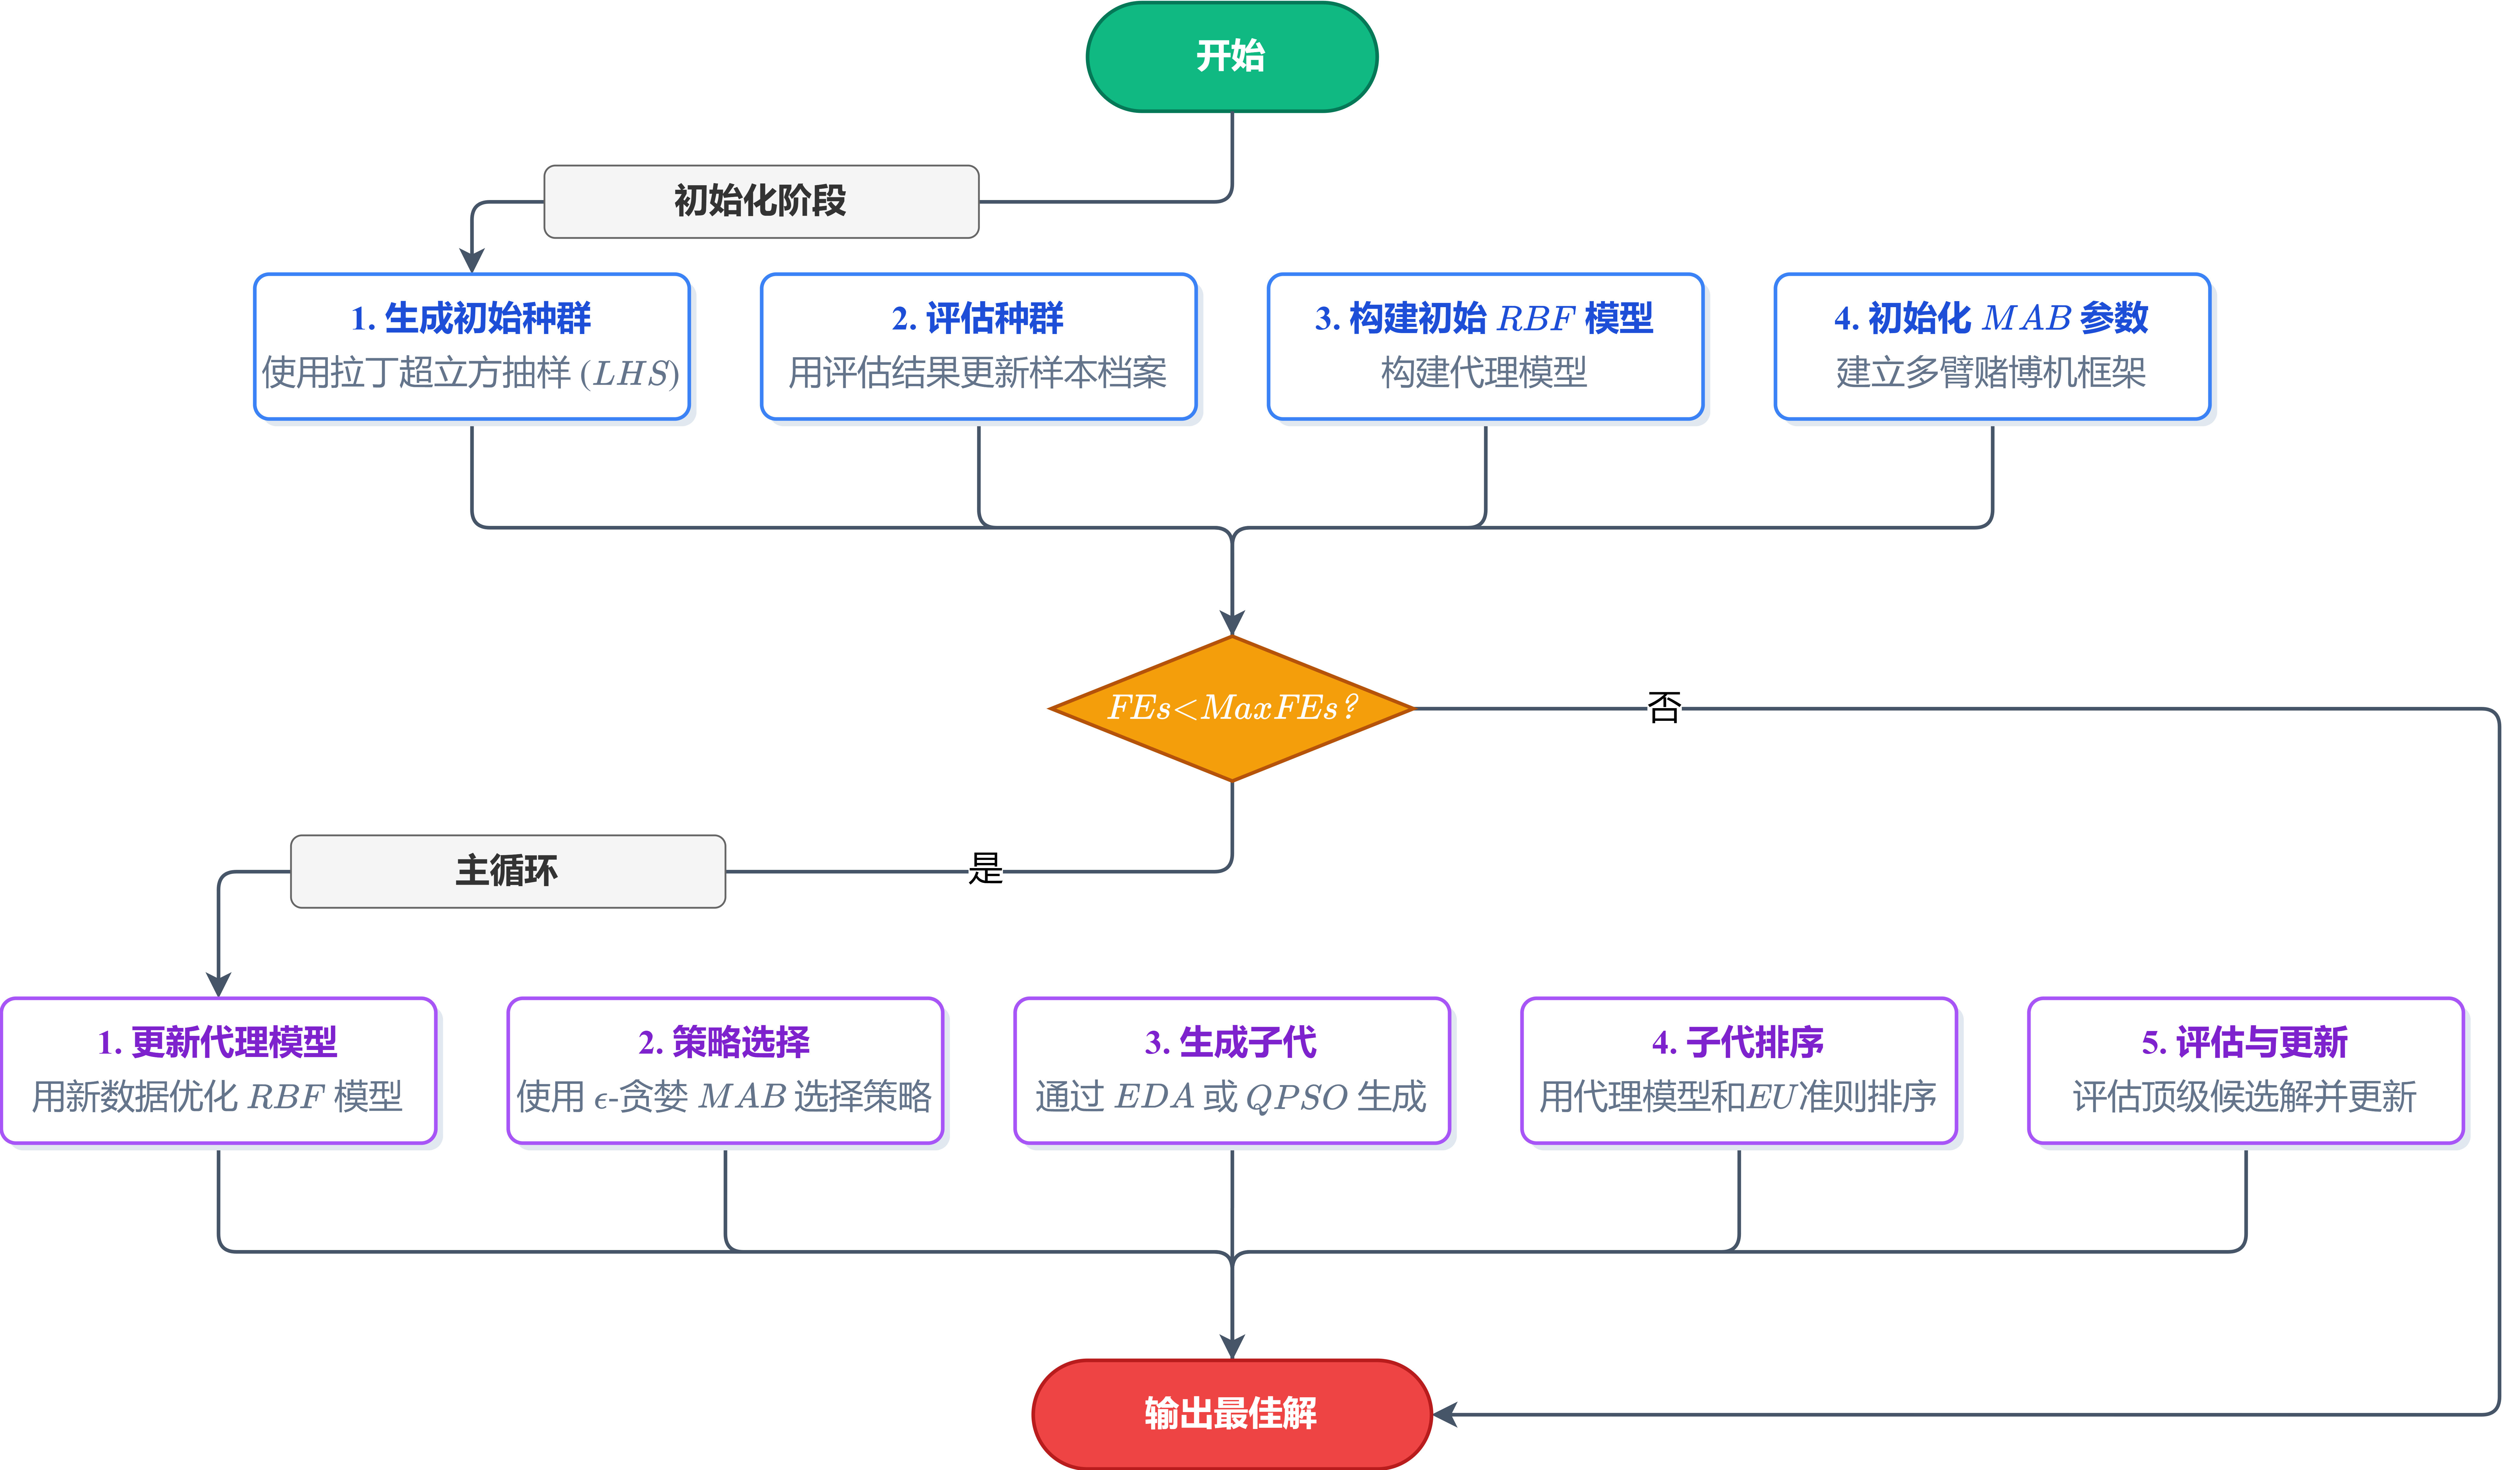
\includegraphics[width=\linewidth]{figures/chapter5/BEXEAStructure.png}
    \bicaption{BEXEA算法流程图}{Flowchart of the BEXEA algorithm}
    \label{fig:bexea_BEXEA}
\end{figure}

\subsection{多臂赌博机驱动的自适应搜索}
在线策略选择机制已被证明能够根据优化过程中的即时反馈，比静态分配更有效地平衡探索与开发\cite{xie2023surrogate,gong2024surrogate}。通过将$\epsilon$-贪心MAB嵌入SAEA，本章实现了EDA与QPSO策略的在线切换，并辅以停滞检测机制以增强算法的跳出能力。

具体实现中，策略选择被抽象为二臂赌博机问题。在每次迭代周期内，算法根据策略评分和探索概率选择执行动作。在获得新解的评估结果后，计算即时奖励并更新对应策略的价值估计$Q(a)$。

本章采用的$\epsilon$-贪心选择逻辑如下：
\begin{equation}
a_t =
\begin{cases}
\argmax\limits_a Q_t(a) & \text{with probability } 1-\epsilon \\
\text{random strategy} & \text{with probability } \epsilon
\end{cases}
\end{equation}
其中$\epsilon$设在0.1至0.3之间，通过维持适度的探索行为，防止算法过早陷入特定策略。

奖励函数的设计不仅考虑了适应度值的直接改进量，还结合了策略特有的贡献。例如在EDA阶段，会额外奖励能够提升种群多样性的搜索行为；而在QPSO阶段，则将解的可解释性评分纳入考量。这种多准则奖励机制使得算法能更精准地识别不同策略在特定搜索阶段的价值。

为了兼顾历史表现与近期收益，价值更新采用了指数近因加权平均。当搜索进程遭遇停滞（即连续若干次迭代未发现更优解）时，算法会主动上调探索率，强制尝试非贪心策略，从而提升全局搜索的活力。相比传统固定参数，这种动态调节策略更契合复杂优化问题在不同阶段对搜索力度的需求变化。

图\ref{fig:bexea_MAB}刻画了这一自适应过程。从初始化零评分开始，算法通过不断循环的“决策-评估-反馈”链条，自动演化出契合当前搜索景观的执行模式，在收敛效率与解的质量之间寻求最佳平衡。

\begin{figure}[ht]
    \centering
    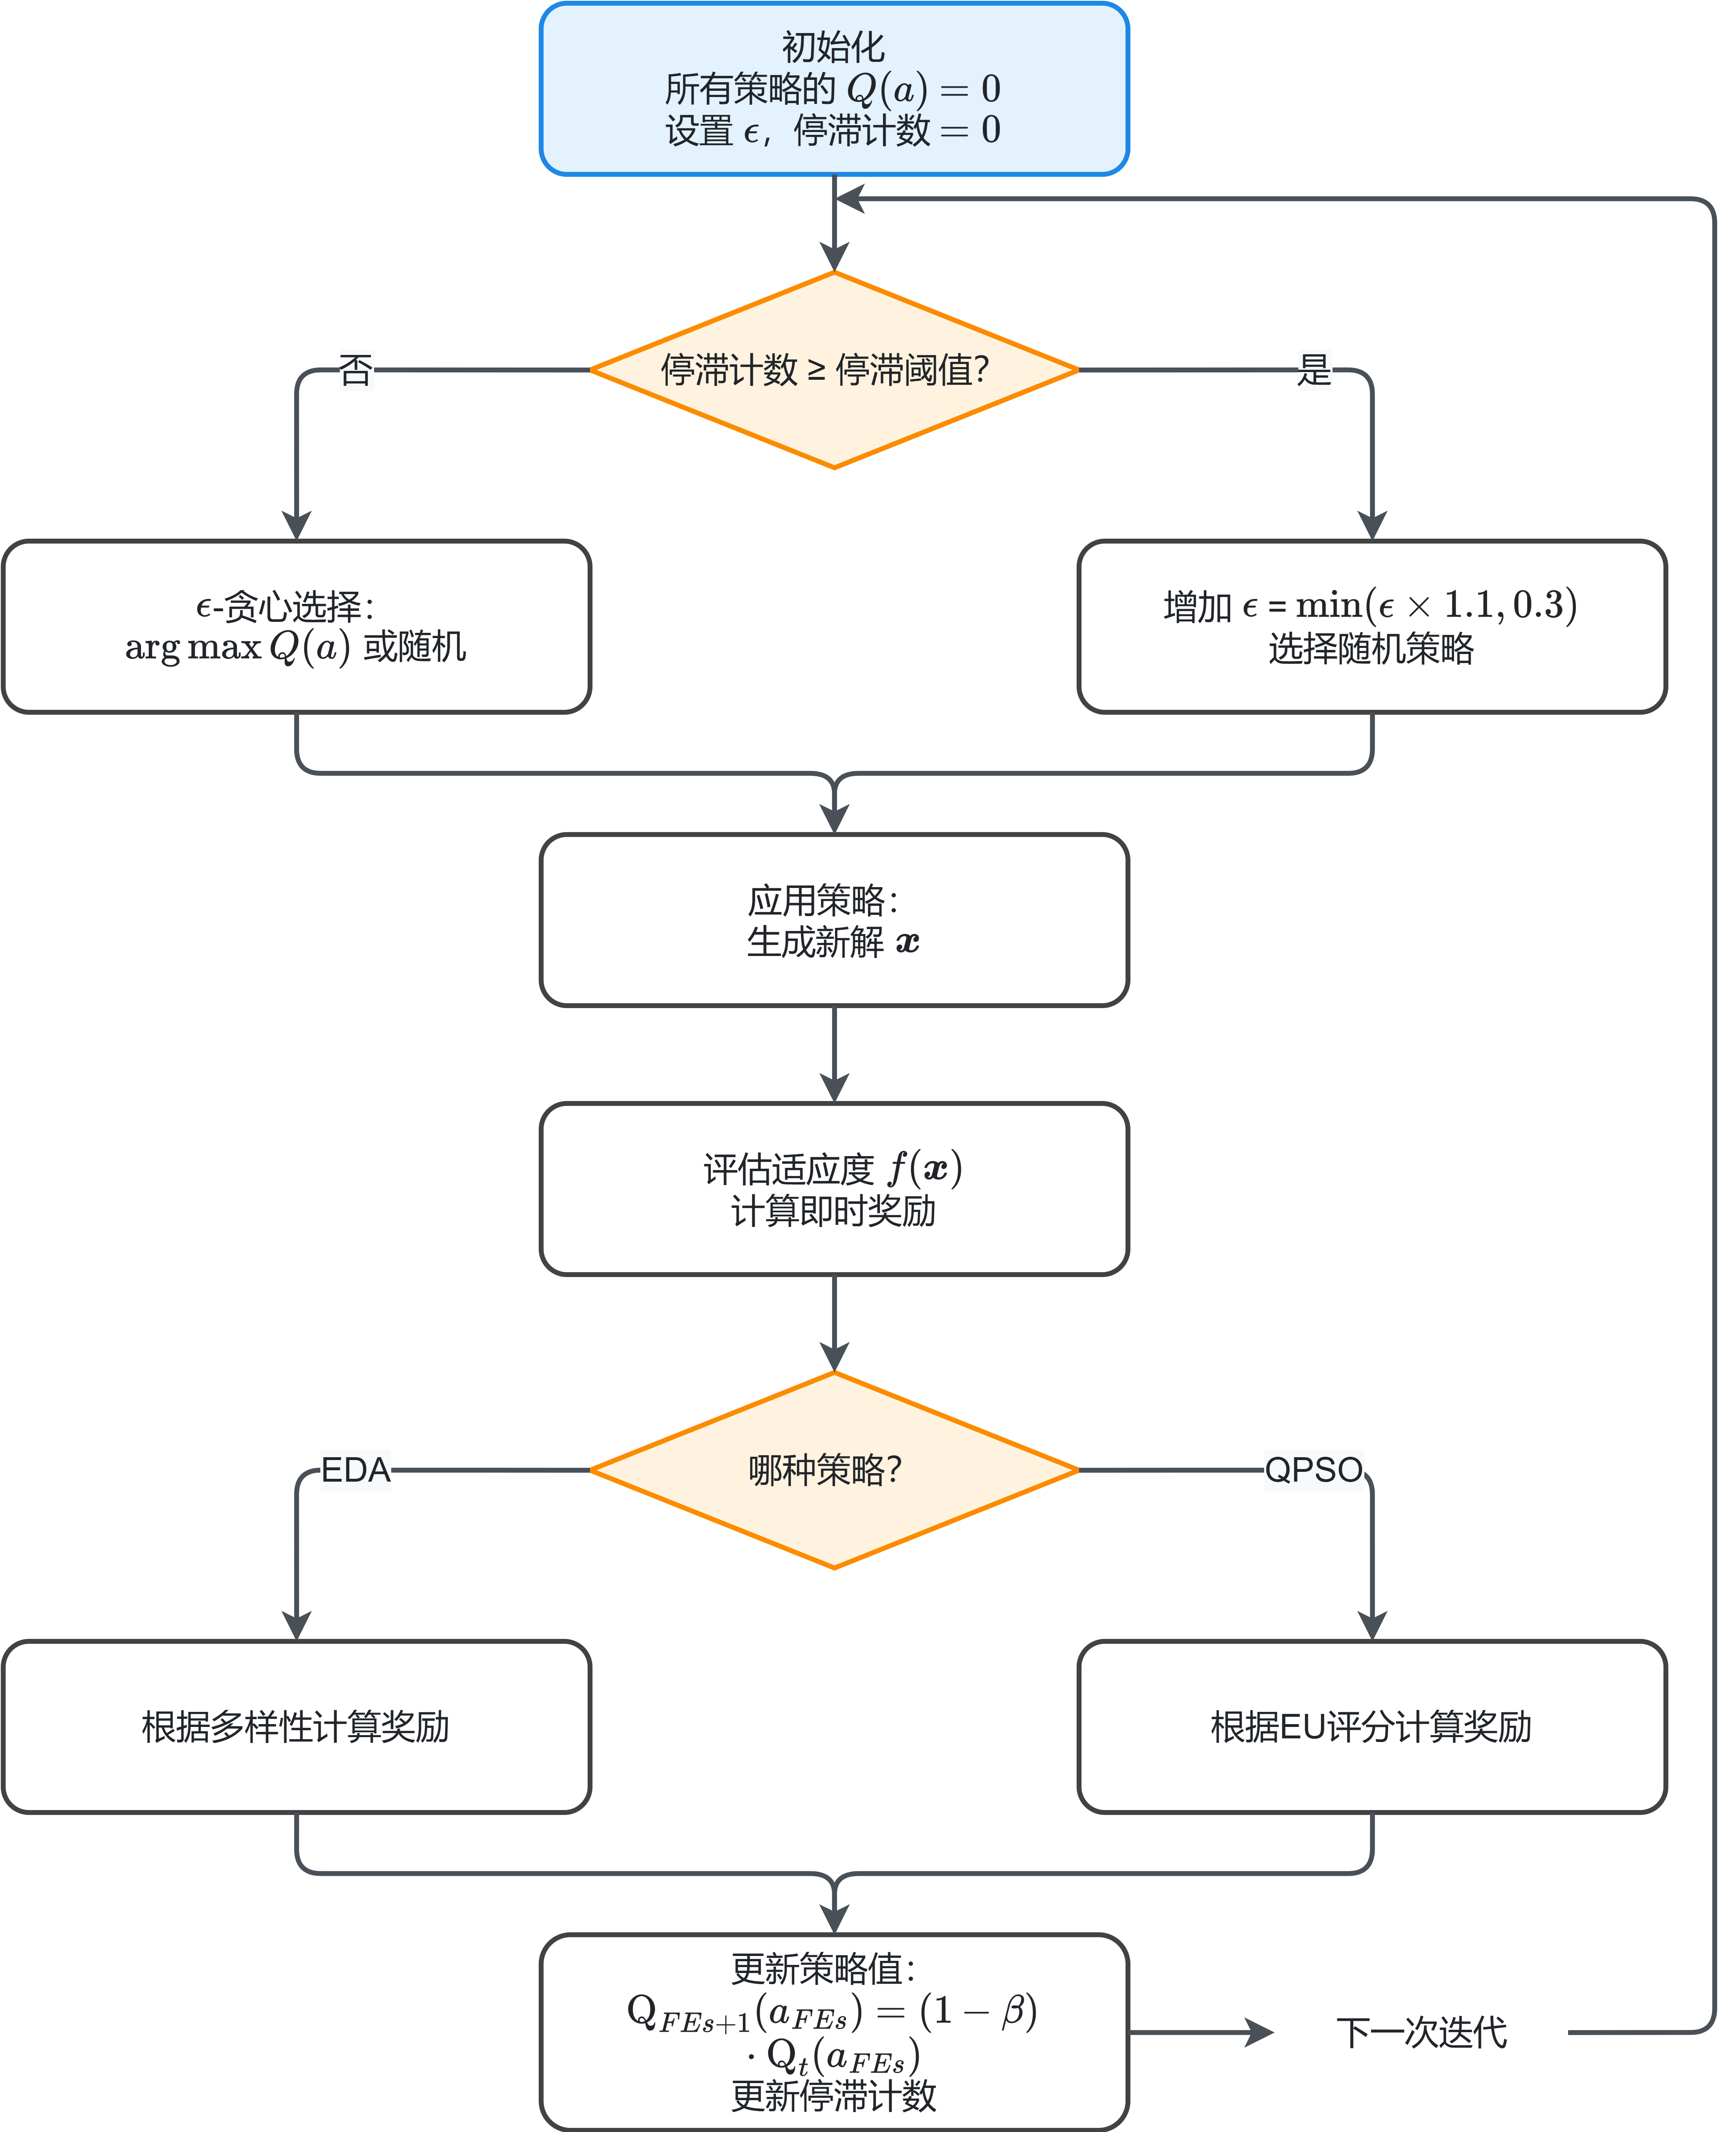
\includegraphics[width=\linewidth]{figures/chapter5/BEXEA-MAB.png}
    \bicaption{BEXEA中多臂赌博机驱动的自适应搜索}{Multi-armed bandit-driven adaptive search in BEXEA}
    \label{fig:bexea_MAB}
\end{figure}

\subsection{可解释不确定性准则}
EU准则融合了贝叶斯优化理论与可解释人工智能的思想，为采样决策提供了一套兼顾预测增量与决策透明度的衡量标准。

对于任一候选解，算法首先在历史档案中选取$\mathcal{K}$个近邻，基于局部数据估计其均值与标准差，进而计算期望改进（EI）。这一过程保证了采样对潜在最优区域的偏好。与此同时，本章创新性地计算了候选解相对于近邻的特征差异分布。受SHAP原理启发，这些差异被视为局部维度的重要性表征。

通过计算特征重要性分布的Shannon熵，可以量化预测判断背后的归因不确定性。高熵值通常意味着该点的预测驱动因素较为模糊，而低熵点则表明其具有更明确的归因依据。

最终形成的EU评价值将EI与反向的熵值相结合，使其表现出独特的优选逻辑：优先选择那些既具有显著改进潜力、又能够被清晰解释的候选区域。这种采样策略不仅有助于提升搜索的针对性，也为后续的工程决策提供了更扎实的可信度。在BEXEA中，EU准则不仅用于候选解的排序筛选，还作为赌博机奖励机制的关键组成部分，引导搜索策略向更具解释力的方向演化。

\begin{figure}[ht]
    \centering
    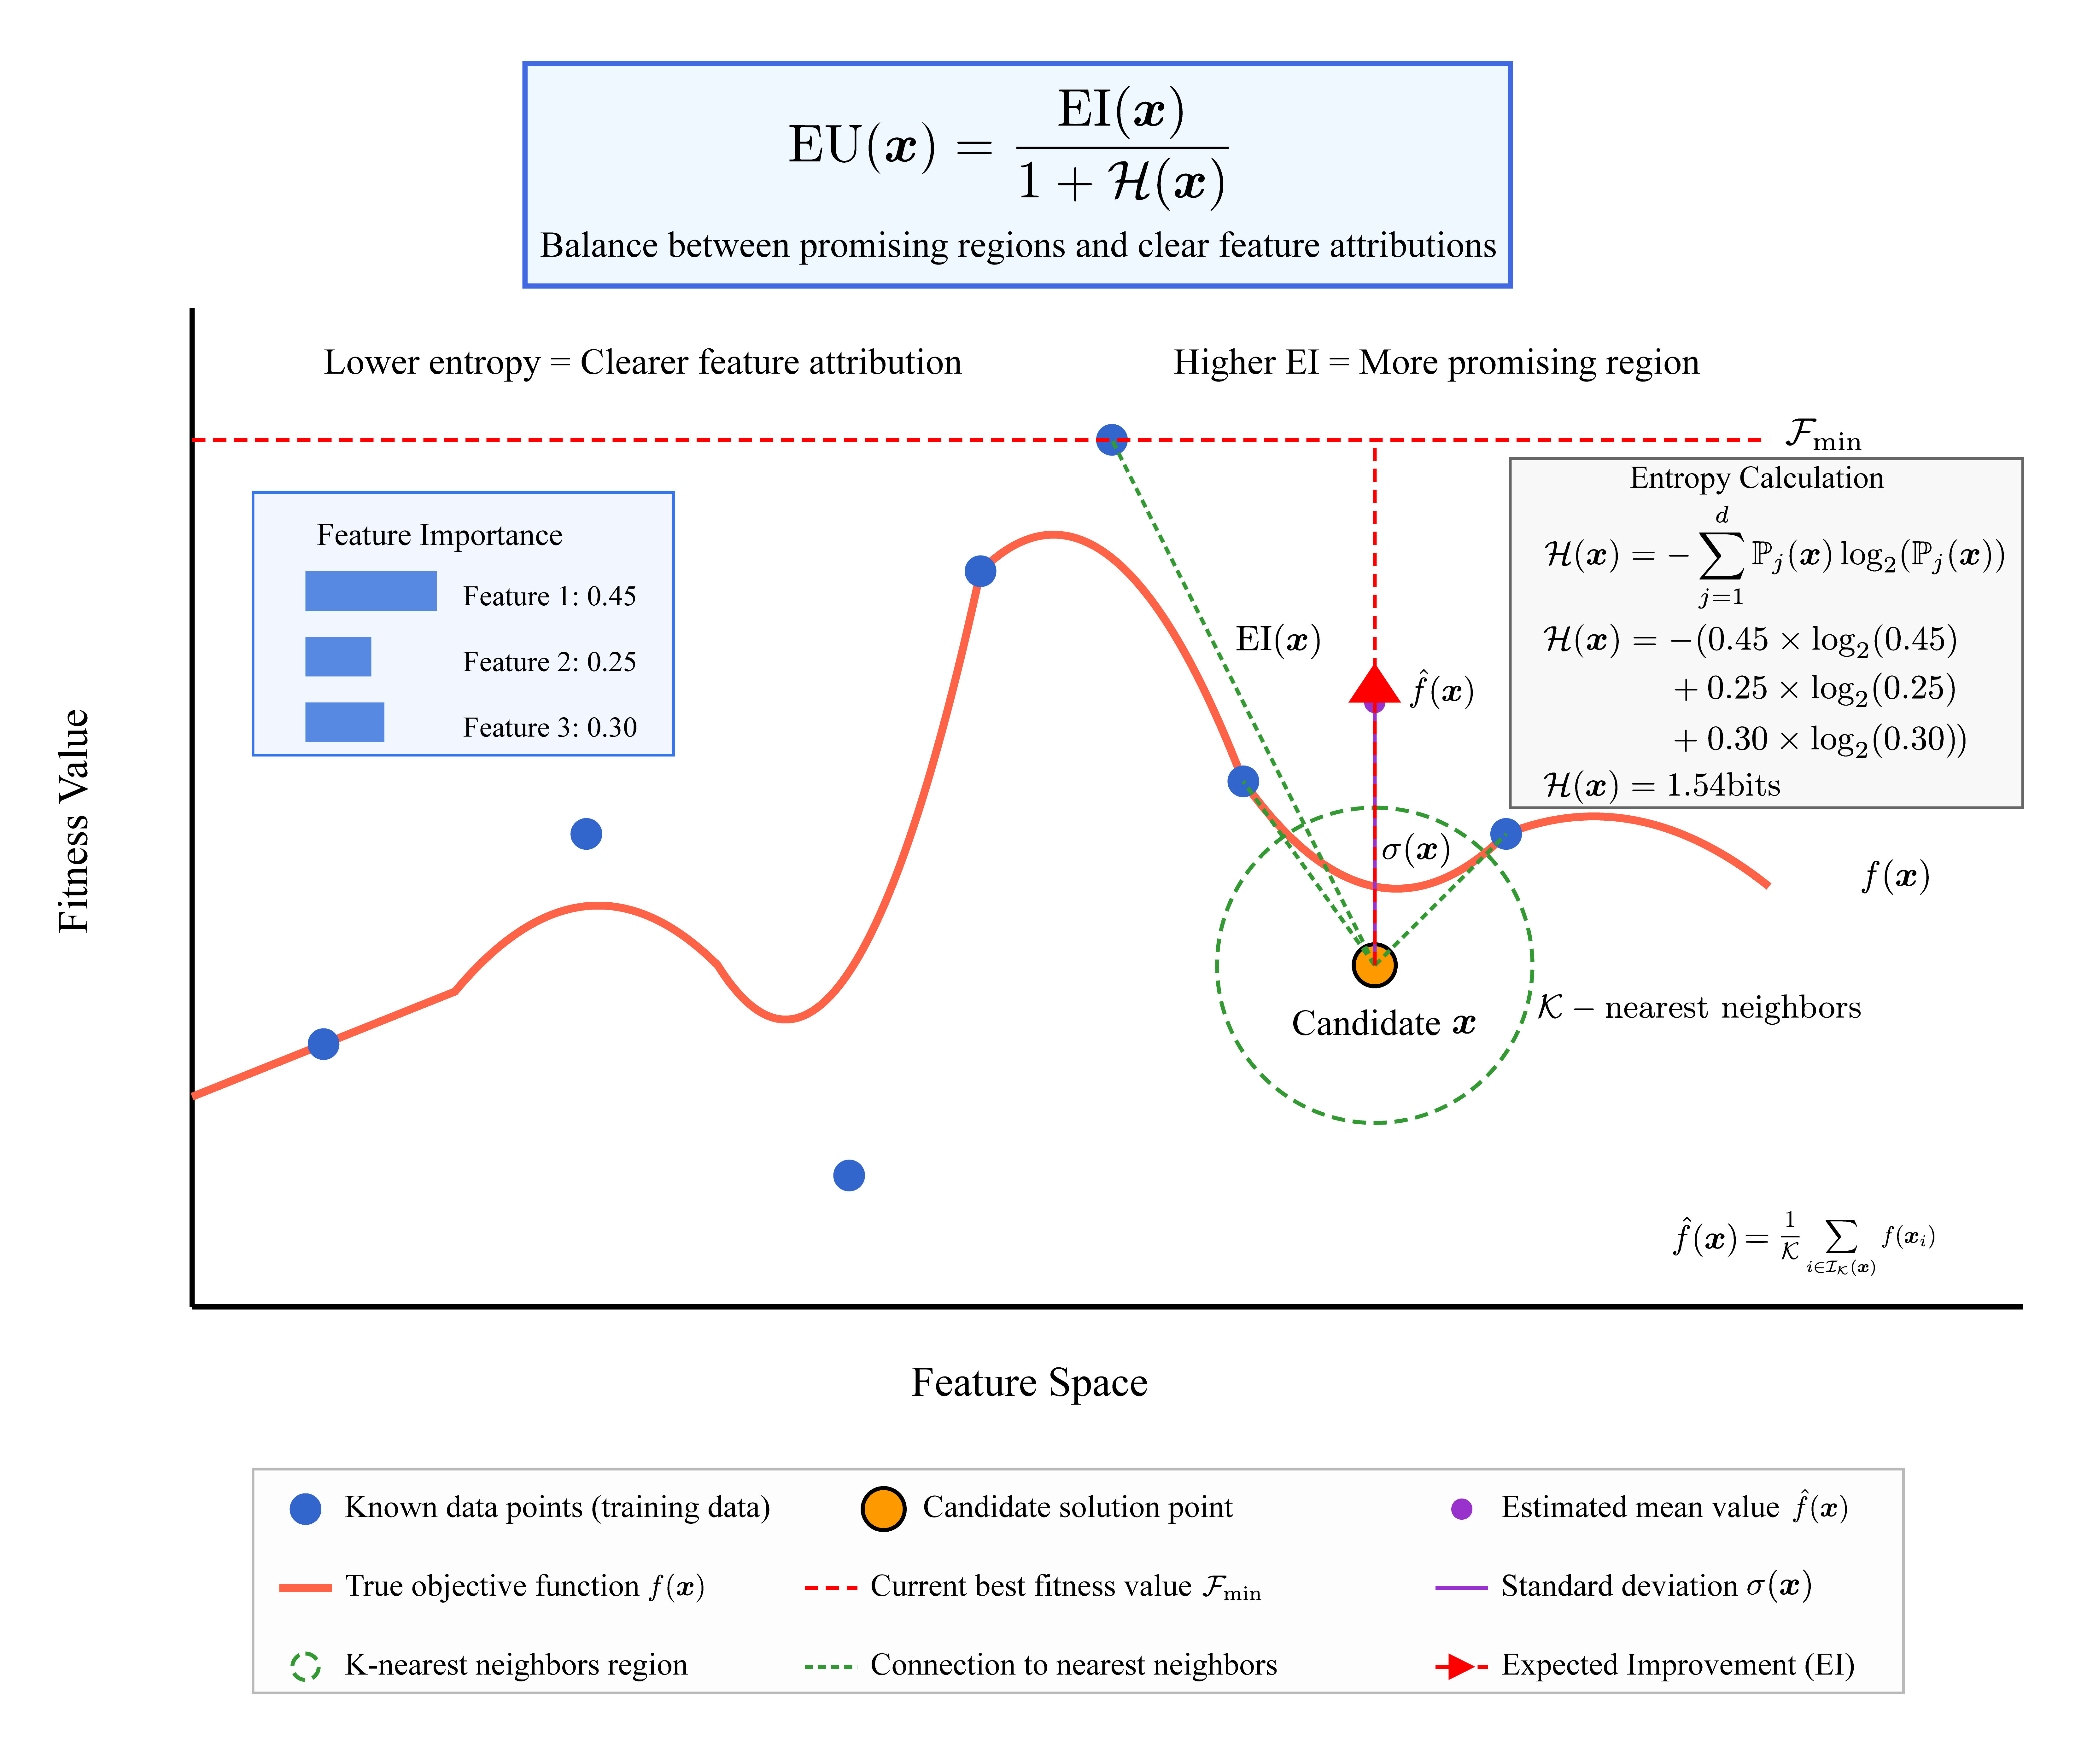
\includegraphics[width=\linewidth]{figures/chapter5/explainable-uncertainty-criteria-legend.png}
    \bicaption{可解释不确定性准则在三维函数上的示意图}{Illustration of the explainable uncertainty criteria on a 3-dimensional function}
    \label{fig:bexea_EU}
\end{figure}

\section{BEXEA的实验研究}

本节首先通过昂贵优化基准问题评估BEXEA的综合性能，随后将其应用于油藏产量优化算例，最后借助消融与参数实验对算法的核心机制进行深入解构。

\subsection{实验设置}

本研究采用了两组各具代表性的基准测试。首先是IEEE CEC 2022测试集（$d=20$），用于考察算法在标准维度下的优化能力。其次是针对高维场景设计的测试套件（$d=50$和$d=100$），涵盖了从简单单峰到复杂多峰旋转、混合等多种函数类型。实验数据的统计分析遵循第二章所述流程，统一采用Friedman检验与Wilcoxon秩和检验（置信水平$\alpha=0.05$），以确保对比结论的可靠性。

在竞争算法的选择上，本章挑选了TSA-BFEA、KTA2、DESO等七种具有代表性的先进SAEAs。为保证对比的公平性，所有算法的参数均严格执行原作者的推荐设置。BEXEA自身的衰减因子和近邻数分别固定为0.3和8。在所有测试任务中，函数评估上限设为1000次，每项测试均独立运行20次。

\subsection{油藏问题描述}

为了评估算法在工程实战中的表现，本章将其引入油藏产量优化任务中。该问题的核心是寻找最优的井控方案，以在权衡注水与生产成本后实现净现值（NPV）的最大化。

在本项研究中，采用经典的Egg模型进行测试。该系统包含8口注水井与4口生产井，构成了一个40维的决策空间。由于单次油藏模拟涉及到多相流偏微分方程的求解，计算代价极高。在这类真实昂贵场景下，算法被要求在仅有的200次评估预算内找到尽可能优的控制方案，这对其样本利用效率提出了极为苛刻的要求。

\begin{figure}[htbp]
    \centering
    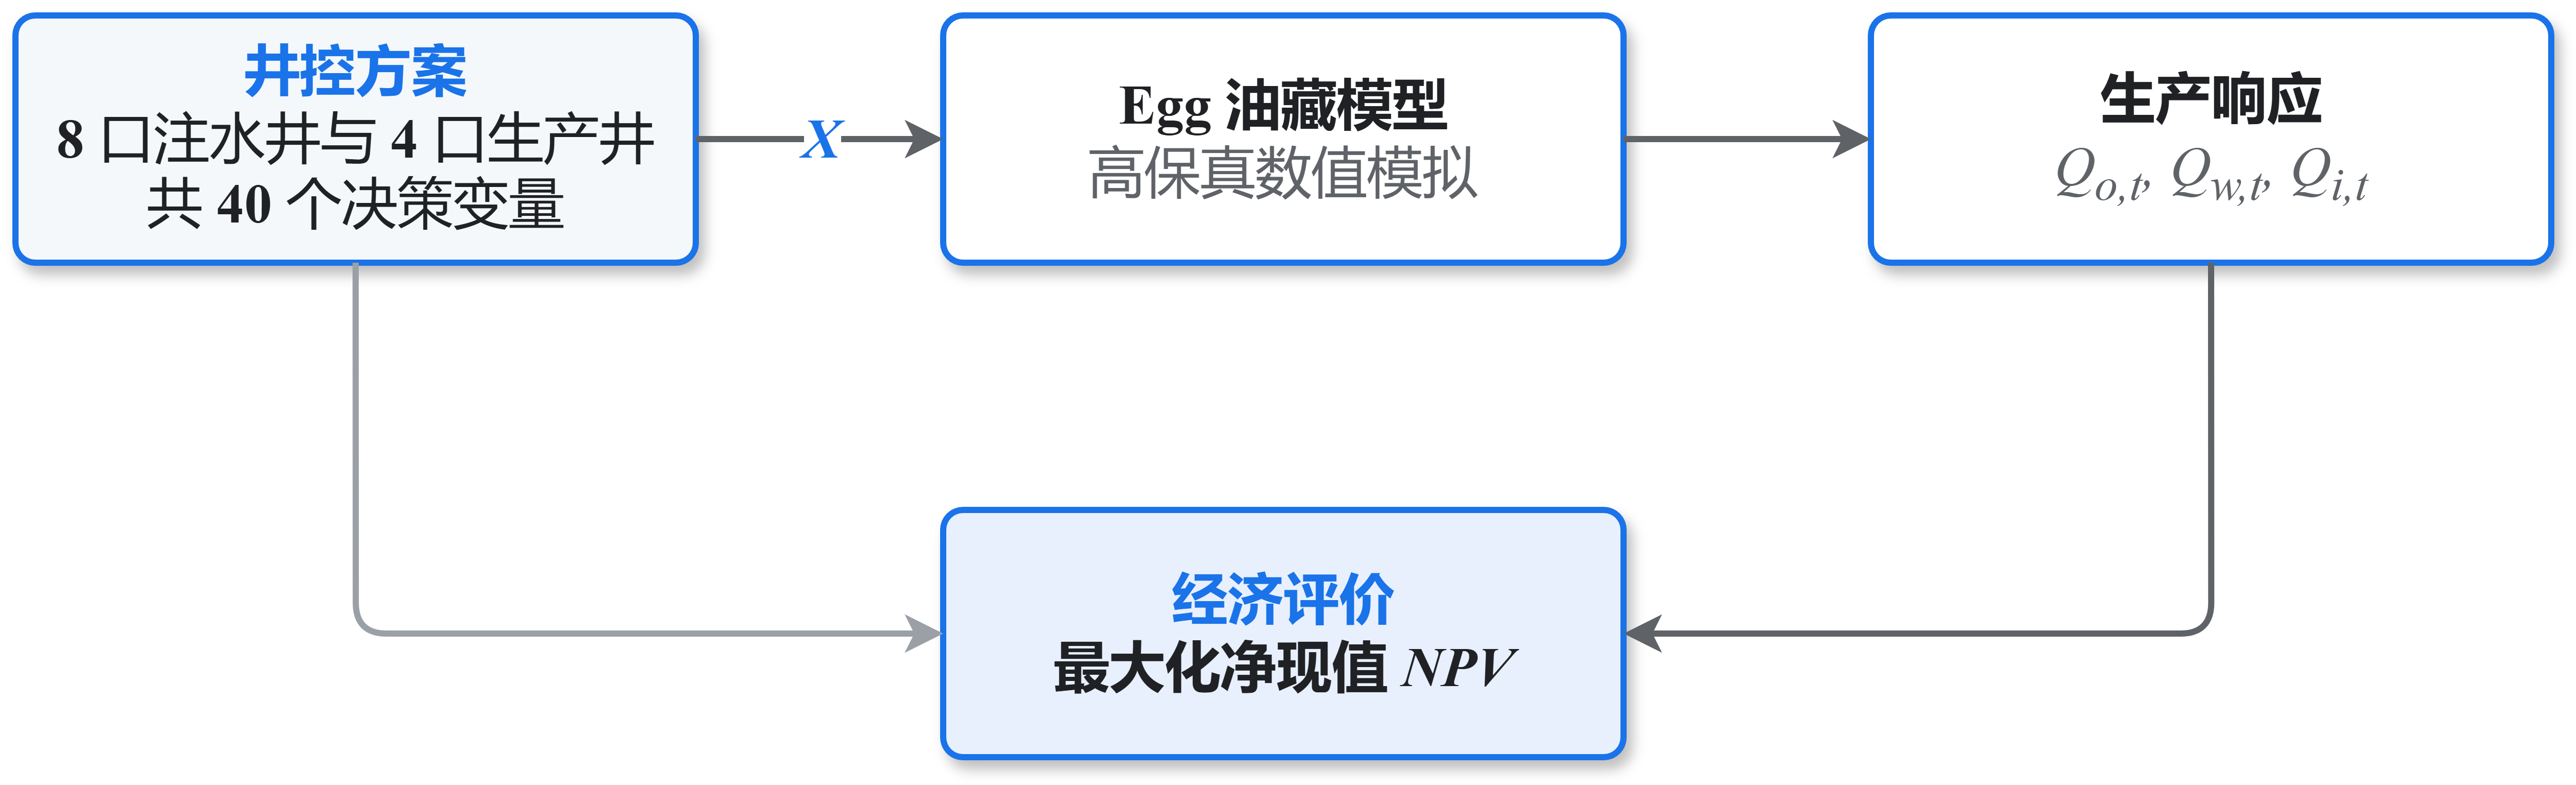
\includegraphics[width=0.86\textwidth]{figures/chapter5/BEXEA_application_workflow_refined.drawio.png}
    \bicaption{油藏产量优化问题示意图}{Schematic of the oil reservoir production optimization problem}
    \label{fig:bexea_oil_problem}
\end{figure}

如图\ref{fig:bexea_oil_problem}所示，井控决策方案经过高保真模拟器处理，输出产量数据，最终由经济模型折算为NPV。整个流程充分体现了昂贵优化问题中高开销、强非线性以及时空高度耦合的复杂特性。

\subsection{实验结果与分析}

本节将逐一分析BEXEA在基础函数测试与工程算例中的表现。

\subsubsection{昂贵优化基准实验}

表\ref{t:bexea_CEC22_Table}与表\ref{t:bexea_CEC05_Table}呈现了详细的对比数据。

\begin{table}[htbp]
\centering
\bicaption{BEXEA与竞争算法在IEEE CEC 2022测试套件上的比较结果（$d=20$）}{Comparison result of BEXEA and its competitors on IEEE CEC 2022 test suite with $d=20$}
\label{t:bexea_CEC22_Table}
\resizebox{\textwidth}{!}{\begin{tabular}{lccccc}
\toprule
Problem & TSA-BFEA & KTA2 & DESO & MS-MTO & BEXEA \\
\midrule
F1 & 5.933E+04(1.38E+04)= & 2.836E+06(8.60E+06)= & 6.914E+04(1.44E+04)= & 7.342E+04(1.76E+04)= & {5.349E+04(1.70E+04)} \\
F2 & 1.778E+03(3.53E+02)= & 2.717E+03(3.24E+03)+ & 2.464E+03(6.82E+02)+ & 3.040E+03(7.88E+02)+ & \textbf{4.536E+02(8.78E+00)} \\
F3 & 6.720E+02(9.72E+00)+ & 6.769E+02(3.97E+01)+ & 6.746E+02(1.46E+01)+ & 6.993E+02(9.61E+00)+ & \textbf{6.118E+02(1.11E+01)} \\
F4 & 9.915E+02(1.83E+01)+ & 9.980E+02(7.02E+01)+ & 9.828E+02(2.67E+01)+ & 1.064E+03(3.46E+01)+ & \textbf{8.363E+02(1.14E+01)} \\
F5 & 5.072E+03(6.50E+02)+ & 6.314E+03(5.22E+03)+ & 4.401E+03(1.33E+03)+ & 9.870E+03(2.43E+03)+ & \textbf{1.094E+03(2.06E+02)} \\
F6 & 1.418E+09(7.00E+08)+ & 1.484E+09(2.16E+09)+ & 1.297E+09(6.03E+08)+ & 4.444E+09(1.53E+09)+ & \textbf{3.665E+03(1.46E+03)} \\
F7 & 2.253E+03(5.94E+01)+ & 2.422E+03(1.51E+02)+ & 2.270E+03(7.88E+01)+ & 2.469E+03(1.18E+02)+ & \textbf{2.127E+03(7.97E+01)} \\
F8 & 2.767E+03(2.62E+02)+ & 3.011E+03(4.58E+02)+ & 2.450E+03(1.20E+02)+ & 2.787E+03(1.23E+02)+ & \textbf{2.279E+03(5.88E+01)} \\
F9 & 2.970E+03(1.04E+02)+ & 3.011E+03(5.97E+02)+ & 3.231E+03(2.91E+02)+ & 3.298E+03(1.96E+02)+ & \textbf{2.496E+03(1.55E+01)} \\
F10 & 5.217E+03(2.05E+03)+ & 6.669E+03(1.93E+03)+ & 6.120E+03(1.96E+03)+ & 8.185E+03(5.66E+02)+ & \textbf{3.558E+03(1.12E+03)} \\
F11 & 8.254E+03(7.23E+02)+ & 9.330E+03(3.76E+03)+ & 8.174E+03(7.03E+02)+ & 9.234E+03(1.08E+03)+ & \textbf{2.902E+03(6.16E-01)} \\
F12 & 3.488E+03(1.43E+02)+ & 3.814E+03(4.00E+02)+ & 3.991E+03(1.93E+02)+ & 3.642E+03(1.54E+02)+ & \textbf{3.006E+03(3.70E+01)} \\
\midrule
Ranking & 4.2 & 6.3 & 4.5 & 6.8 & \textbf{1.1} \\
+/-/= & 10/0/2 & 11/0/1 & 11/0/1 & 11/0/1 & NA \\
\bottomrule
\end{tabular}}

\vspace{4pt}
\resizebox{\textwidth}{!}{\begin{tabular}{lcccc}
\toprule
Problem & ESA & eToSADE & SHPSO & BEXEA \\
\midrule
F1 & 7.466E+04(2.64E+04)= & \textbf{5.206E+04(1.10E+04)=} & 5.470E+04(1.52E+04)= & {5.349E+04(1.70E+04)} \\
F2 & 7.269E+03(1.78E+03)+ & 1.441E+03(3.16E+02)= & 4.944E+02(2.15E+01)= & \textbf{4.536E+02(8.78E+00)} \\
F3 & 7.015E+02(8.62E+00)+ & 6.689E+02(1.01E+01)+ & 6.239E+02(5.83E+00)+ & \textbf{6.118E+02(1.11E+01)} \\
F4 & 1.070E+03(2.02E+01)+ & 9.944E+02(1.13E+01)+ & 9.428E+02(1.55E+01)+ & \textbf{8.363E+02(1.14E+01)} \\
F5 & 9.096E+03(1.20E+03)+ & 5.360E+03(9.01E+02)+ & 1.264E+03(2.60E+02)+ & \textbf{1.094E+03(2.06E+02)} \\
F6 & 6.796E+09(2.12E+09)+ & 7.825E+08(3.00E+08)+ & 4.465E+07(2.12E+07)= & \textbf{3.665E+03(1.46E+03)} \\
F7 & 2.365E+03(8.57E+01)+ & 2.297E+03(6.38E+01)+ & 2.213E+03(6.14E+01)+ & \textbf{2.127E+03(7.97E+01)} \\
F8 & 4.136E+03(2.50E+03)+ & 2.456E+03(9.63E+01)+ & 2.313E+03(6.43E+01)+ & \textbf{2.279E+03(5.88E+01)} \\
F9 & 3.819E+03(4.30E+02)+ & 2.771E+03(5.97E+01)+ & 2.572E+03(3.68E+01)= & \textbf{2.496E+03(1.55E+01)} \\
F10 & 7.003E+03(1.20E+03)+ & 4.280E+03(1.79E+03)+ & 5.182E+03(2.24E+03)+ & \textbf{3.558E+03(1.12E+03)} \\
F11 & 1.299E+04(1.96E+03)+ & 6.569E+03(7.16E+02)= & 3.331E+03(9.54E+01)+ & \textbf{2.902E+03(6.16E-01)} \\
F12 & 4.062E+03(1.78E+02)+ & 3.180E+03(6.87E+01)+ & 3.032E+03(4.10E+01)+ & \textbf{3.006E+03(3.70E+01)} \\
\midrule
Ranking & 7.6 & 3.3 & 2.2 & \textbf{1.1} \\
+/-/= & 11/0/1 & 9/0/3 & 8/0/4 & NA \\
\bottomrule
\end{tabular}}
\end{table}

在IEEE CEC 2022测试中，BEXEA展现出了显著的竞争优势，Friedman平均排名稳居首位（1.1）。在Wilcoxon显著性检验中，绝大多数测试项均支持BEXEA占优。这种稳健的全局寻优能力主要归因于两个方面的协同：首先是MAB机制实现的策略动态平衡，它能依据搜索状态实时倾斜资源，避免了算法在某些阶段出现策略失配；其次是EU准则对评估预算的精准导向，它不仅追求数值上的改进，更侧重于归因清晰的优质区域，从而极大地提高了单次真实评估的含金量。

\begin{figure}
    \centering
    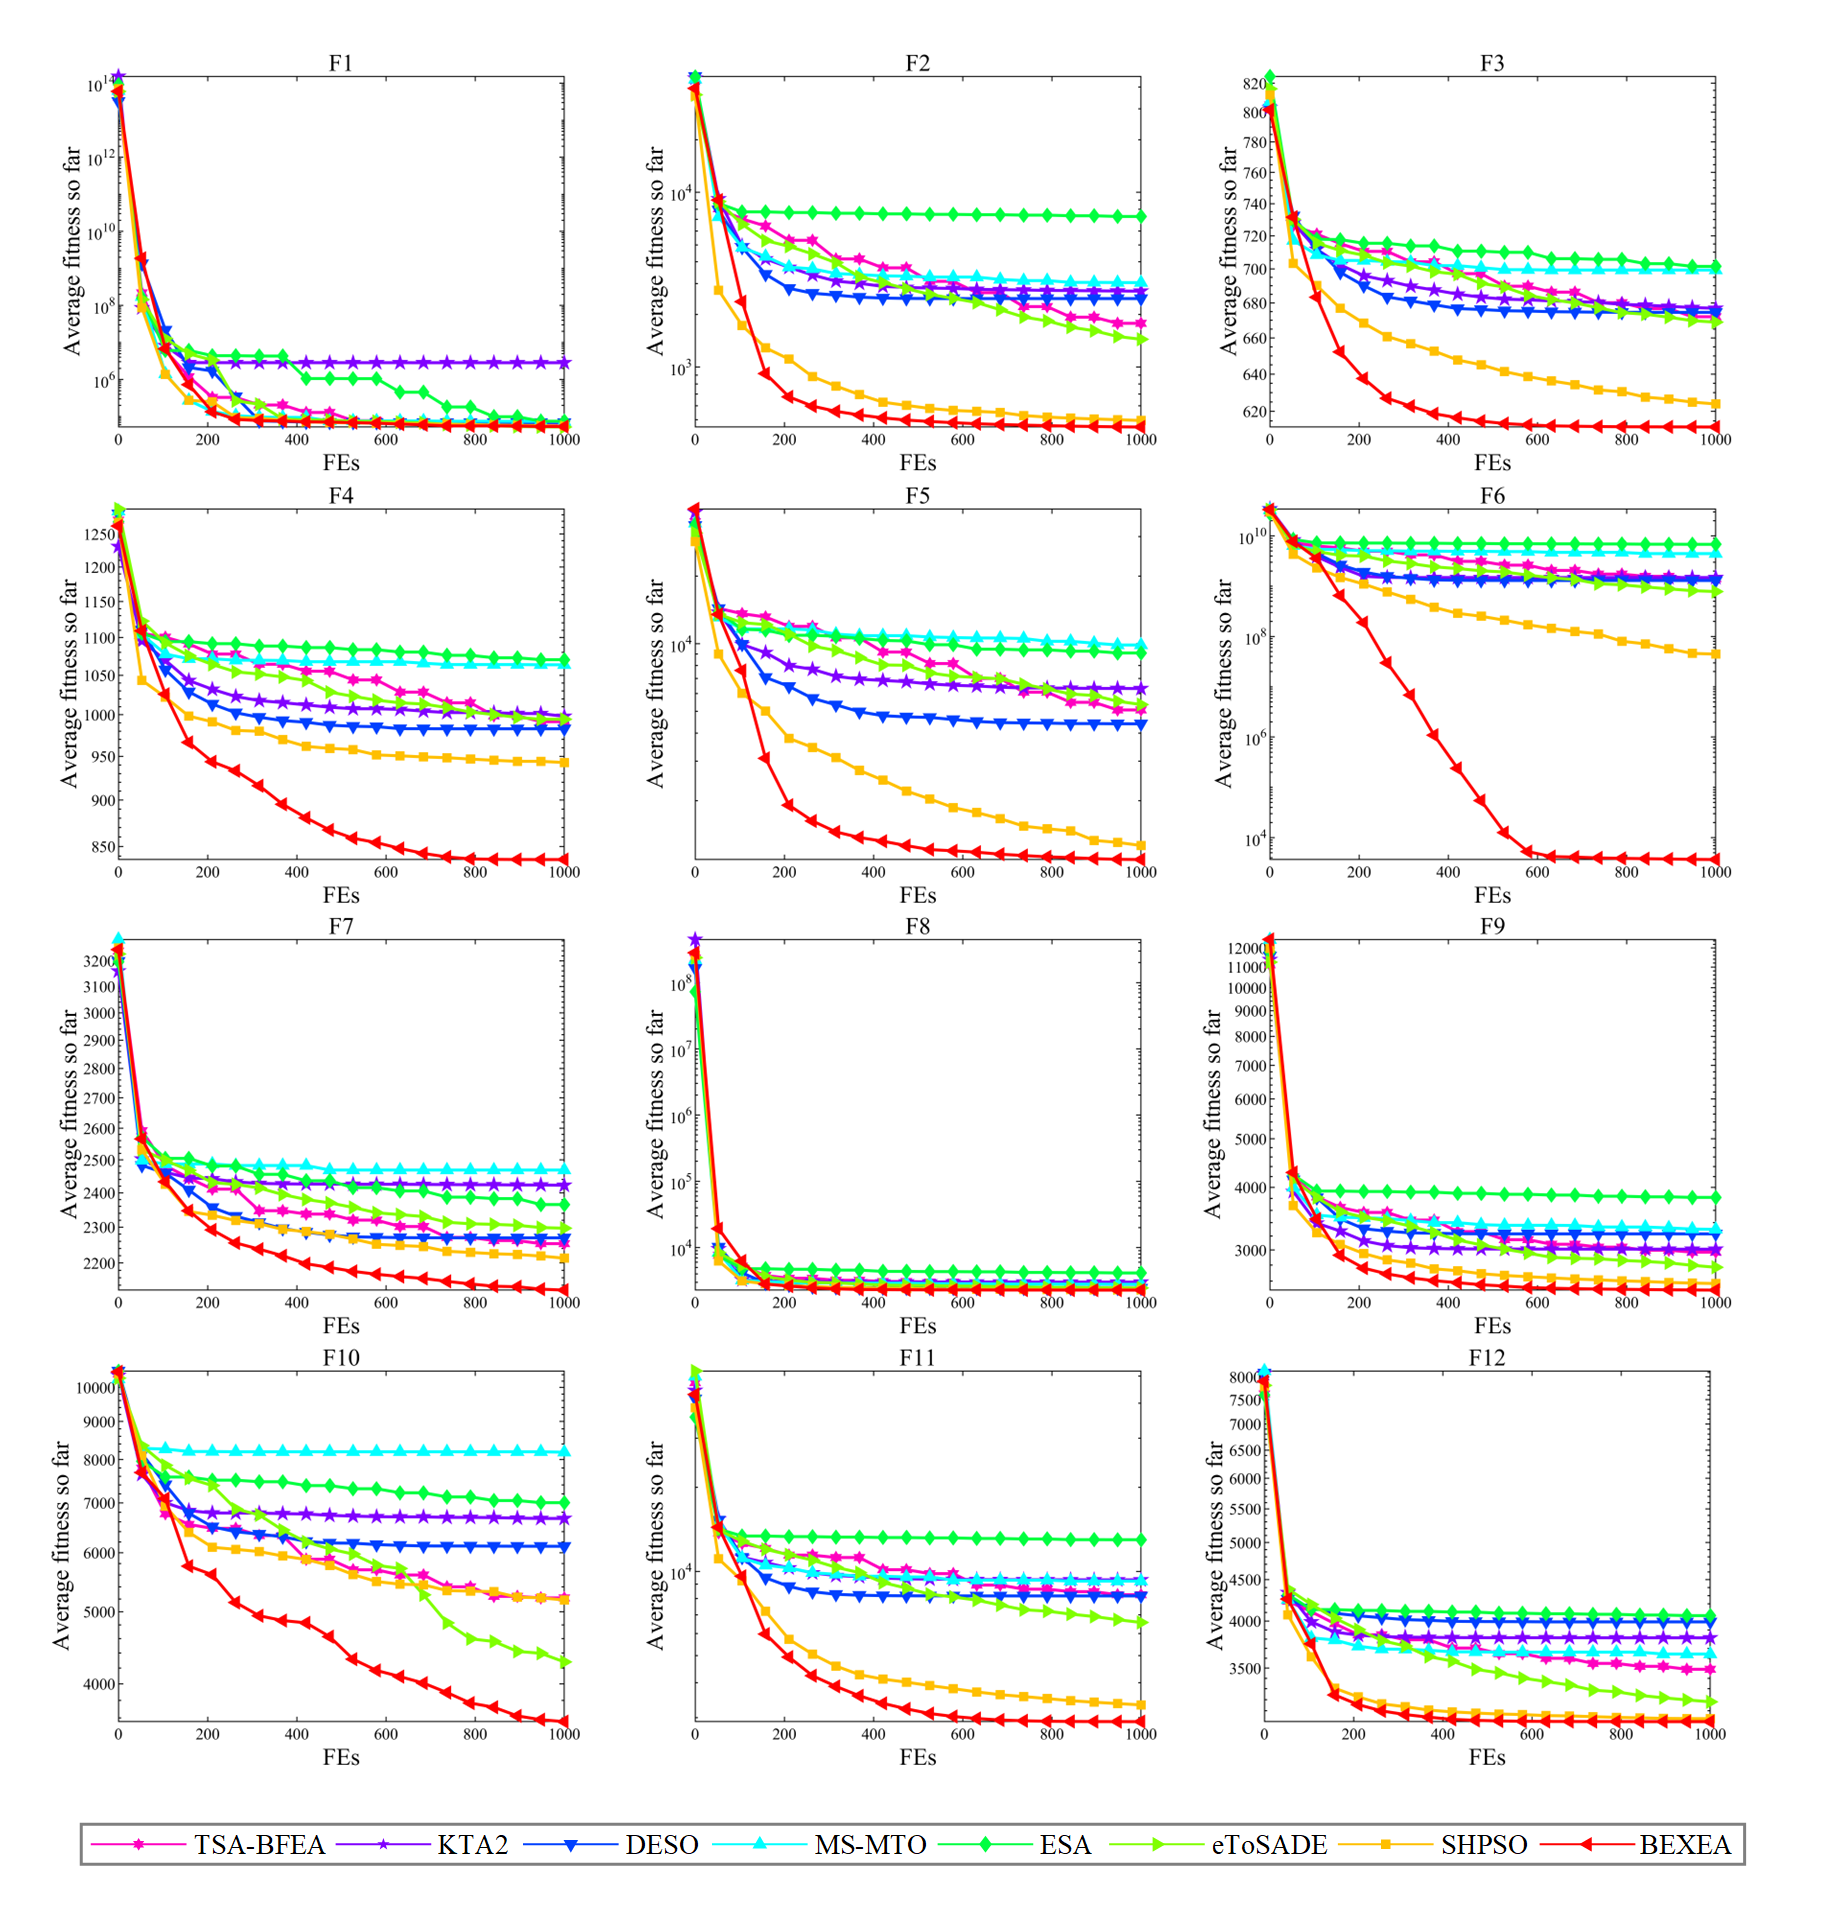
\includegraphics[width=\linewidth]{figures/chapter5/BEXEA-CEC22-CC.png}
    \bicaption{BEXEA与竞争算法在IEEE CEC 2022测试套件上的收敛曲线（$d=20$）}{Convergence curves of BEXEA and its competitors on the IEEE CEC 2022 test suite ($d=20$)}
    \label{fig:bexea_CEC22_CC}
\end{figure}

收敛曲线图\ref{fig:bexea_CEC22_CC}进一步印证了上述观点。在多个极具挑战性的函数（如F4、F6）上，BEXEA均能以更快的速度逼近更低的适应度值，体现了自适应搜索在调节探索与开发力度方面的灵活性。

此外，散点分布图\ref{fig:bexea_CEC22_Plots}显示BEXEA的运行结果更为集中，反映了该算法在不同随机种子下表现出的良好稳定性。

在高维测试场景中（表\ref{t:bexea_CEC05_Table}），BEXEA的优势依然显著。即便维度提升至100维，MAB驱动的策略切换依然能有效应对复杂的搜索景观。尤其是在面对多模态函数时，这种机制能有效维持搜索的多样性，降低陷入局部最优的风险。这充分证明了BEXEA在处理中高维优化任务时具有良好的可扩展性。

\begin{figure}
    \centering
    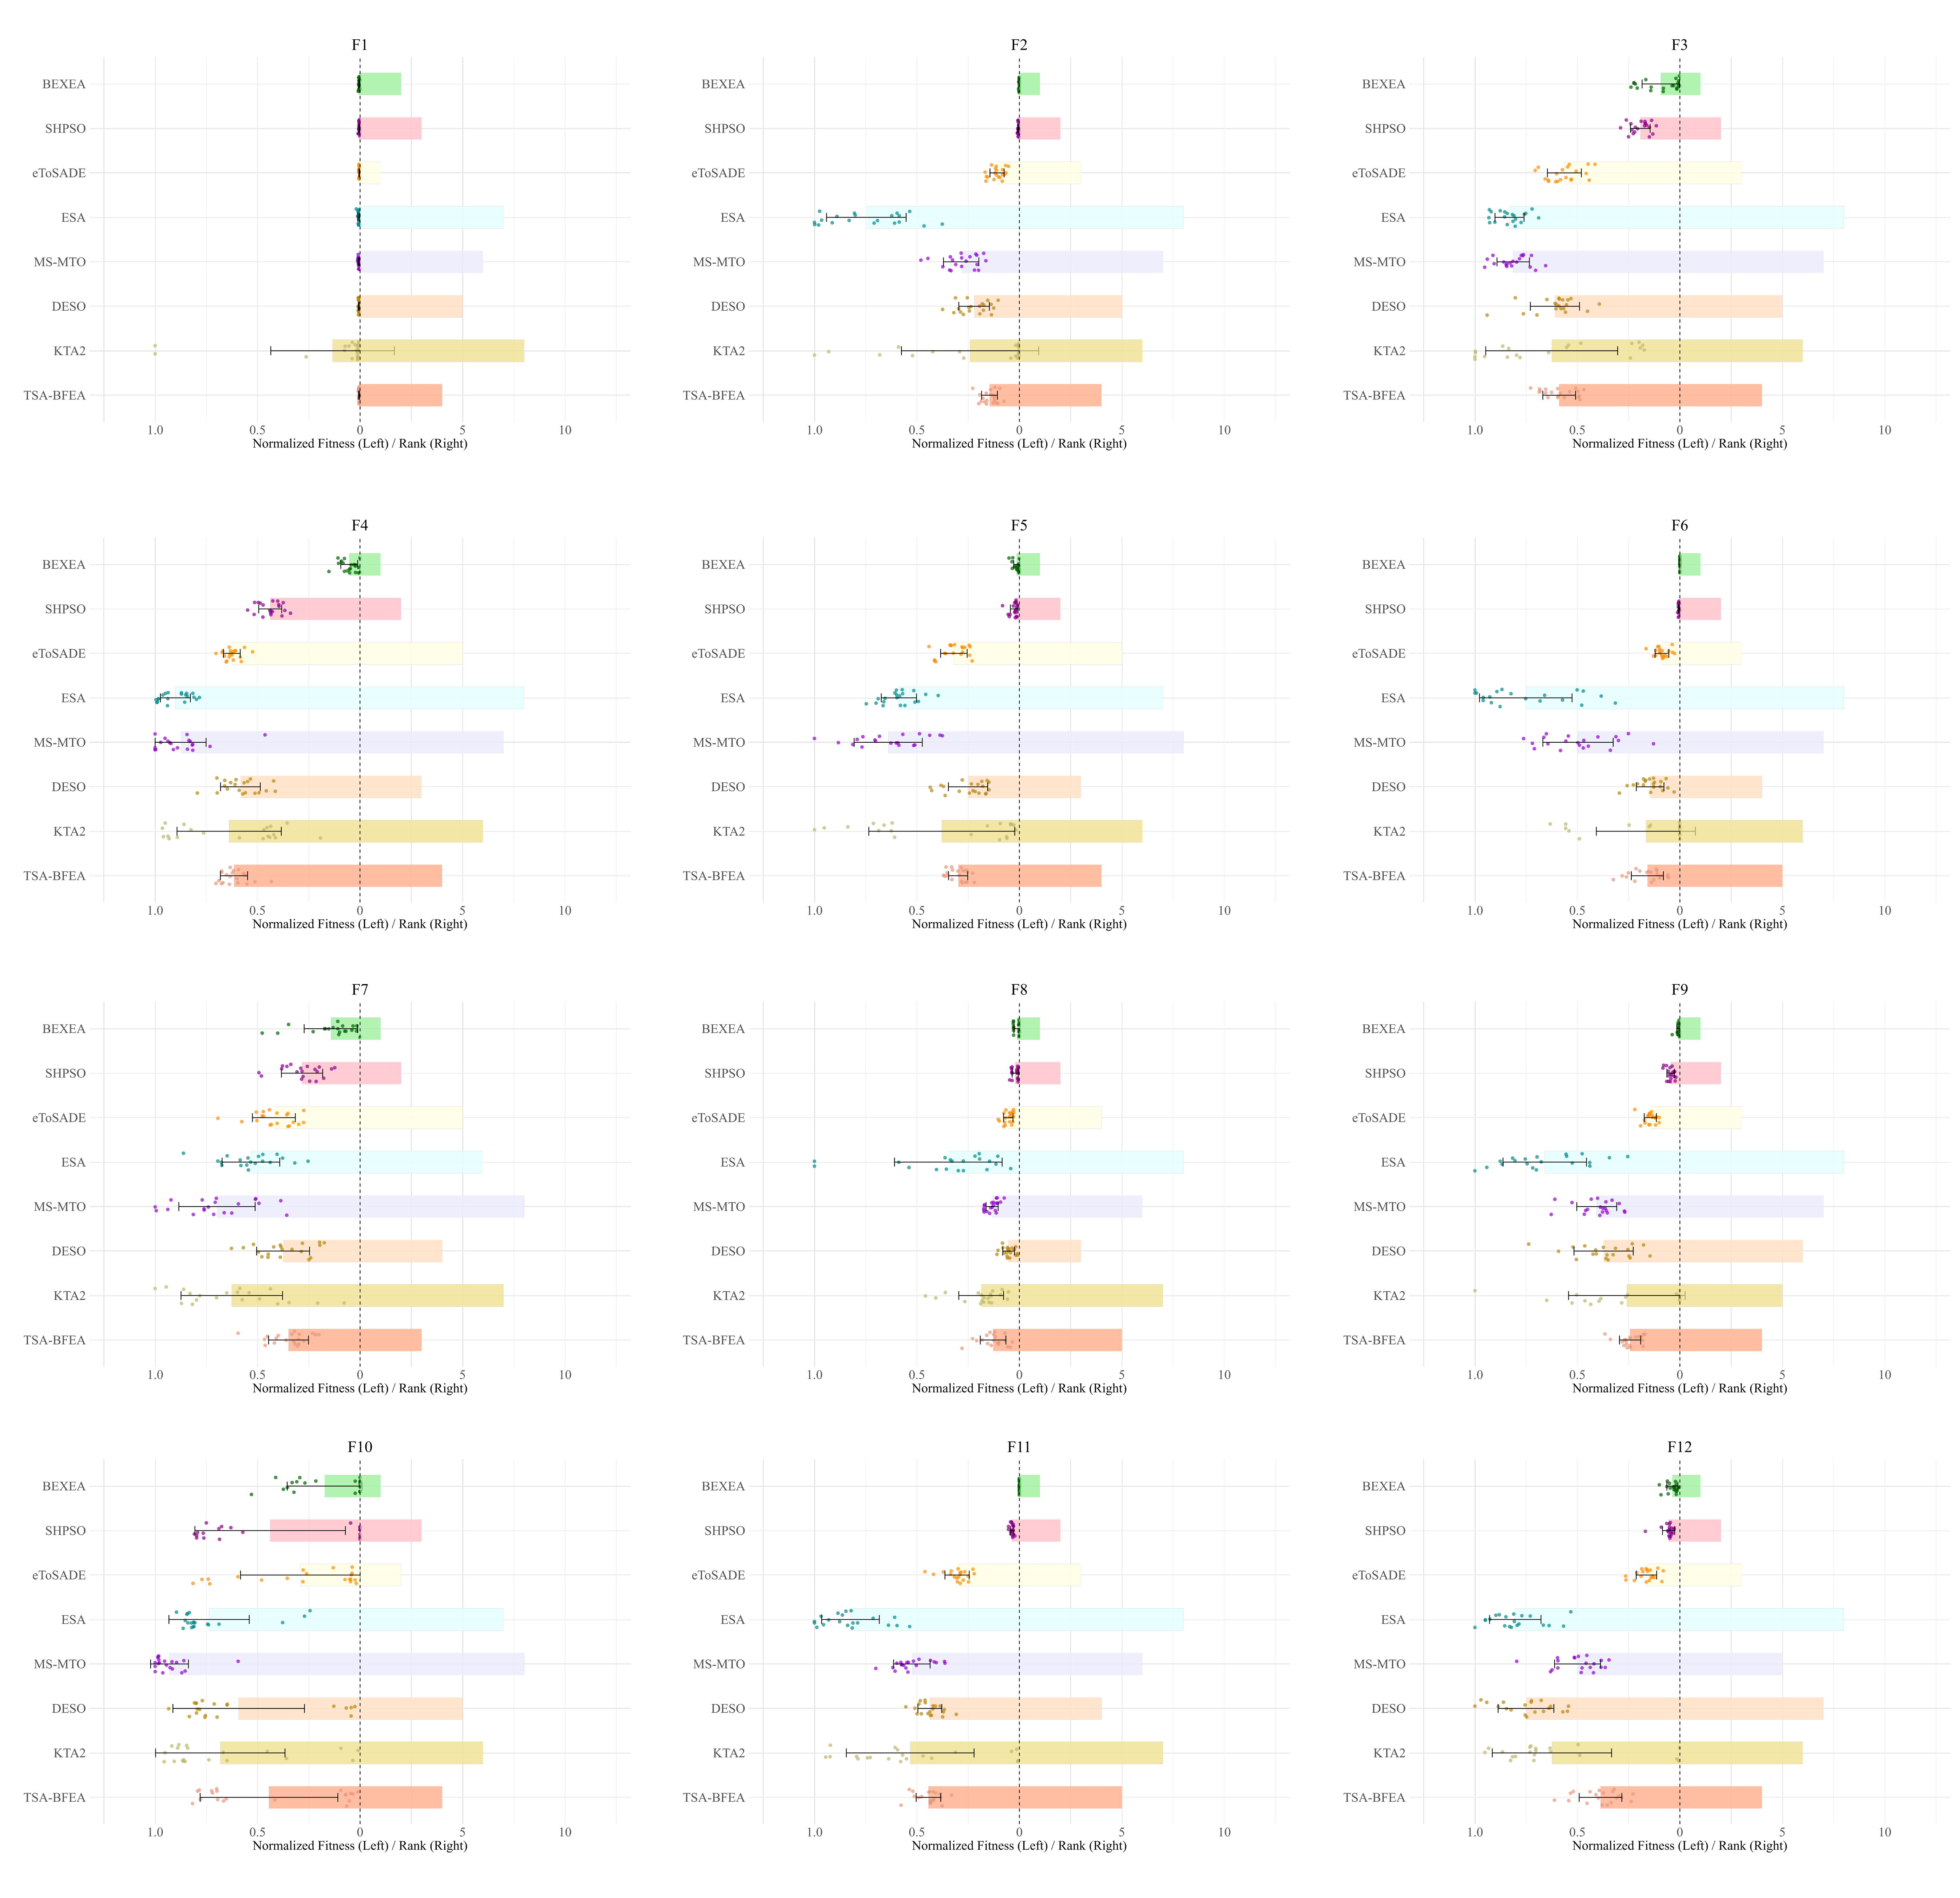
\includegraphics[width=\textwidth]{figures/chapter5/BEXEA-Plots.png}
    \bicaption{BEXEA与竞争算法在IEEE CEC 2022测试套件上的散点图和排名图（$d=20$）}{Combined scatter and rank plots of BEXEA and its competitors on the IEEE CEC 2022 test suite ($d=20$)}
    \label{fig:bexea_CEC22_Plots}
\end{figure}

\begin{table}[htbp]
\centering
\bicaption{BEXEA与竞争算法在昂贵函数测试套件上的比较结果（$d=50$和$d=100$）}{Comparison results of BEXEA and its competitors on the expensive functions test suite with $d=50$ and $d=100$}
\label{t:bexea_CEC05_Table}
\resizebox{\textwidth}{!}{\begin{tabular}{lccccc}
\toprule
Problem & TSA-BFEA & KTA2 & DESO & MS-MTO & BEXEA \\
\midrule
ELLIPSOID-50D & 3.739E+03(3.91E+02)= & 4.084E+03(1.61E+03)= & 1.668E+03(2.36E+02)= & 6.138E+03(7.88E+02)= & \textbf{3.804E+00(1.30E+01)} \\
ELLIPSOID-100D & 2.275E+04(1.98E+03)= & 2.166E+04(6.24E+03)= & 8.687E+03(8.92E+02)= & 3.153E+04(1.45E+03)= & \textbf{3.761E+02(2.63E+02)} \\
ROSENBROCK-50D & 5.220E+03(6.50E+02)+ & 7.696E+03(3.31E+03)+ & 1.681E+03(2.64E+02)+ & 1.003E+04(8.12E+02)+ & \textbf{6.395E+01(3.13E+01)} \\
ROSENBROCK-100D & 1.879E+04(1.76E+03)+ & 1.697E+04(6.02E+03)+ & 4.554E+03(5.54E+02)+ & 2.829E+04(2.75E+03)+ & \textbf{3.355E+02(1.46E+02)} \\
ACKLEY-50D & 1.971E+01(1.32E-01)+ & 2.002E+01(5.83E-01)+ & 1.743E+01(4.96E-01)+ & 2.060E+01(7.61E-02)+ & \textbf{6.695E+00(4.88E+00)} \\
ACKLEY-100D & 2.080E+01(8.07E-02)+ & 2.013E+01(3.05E-01)+ & 1.808E+01(3.29E-01)+ & 2.075E+01(6.40E-02)+ & \textbf{8.868E+00(3.90E+00)} \\
GRIEWANK-50D & 5.739E+02(4.64E+01)+ & 6.260E+02(1.41E+02)+ & 2.535E+02(2.83E+01)+ & 8.116E+02(4.43E+01)+ & 1.384E+01(2.59E+01) \\
GRIEWANK-100D & 1.618E+03(8.46E+01)+ & 1.644E+03(5.32E+02)+ & 6.231E+02(4.40E+01)+ & 2.010E+03(5.44E+01)+ & 8.889E+01(8.31E+01) \\
RASTRIGIN-50D & 5.850E+02(2.68E+01)+ & 6.576E+02(4.98E+01)+ & 4.825E+02(2.63E+01)+ & 7.101E+02(2.21E+01)+ & \textbf{1.108E+02(4.12E+01)} \\
RASTRIGIN-100D & 1.386E+03(5.11E+01)+ & 1.403E+03(1.14E+02)+ & 1.025E+03(4.68E+01)+ & 1.539E+03(3.76E+01)+ & \textbf{4.245E+02(9.07E+01)} \\
SRR-50D & 8.207E+02(7.65E+01)+ & 1.146E+03(1.77E+02)+ & 8.564E+02(6.92E+01)+ & 1.008E+03(6.47E+01)+ & \textbf{-4.131E+01(1.00E+02)} \\
SRR-100D & 2.407E+03(1.11E+02)+ & 2.663E+03(2.02E+02)+ & 1.982E+03(1.14E+02)+ & 2.377E+03(9.53E+01)+ & 1.260E+03(2.04E+02) \\
RHC-50D & 1.359E+03(2.87E+01)+ & 1.461E+03(4.52E+01)+ & 1.369E+03(2.47E+01)+ & 1.452E+03(4.18E+01)+ & 1.089E+03(5.83E+01) \\
RHC-100D & 1.504E+03(5.08E+01)+ & 1.500E+03(2.88E+01)+ & 1.421E+03(1.64E+01)+ & 1.504E+03(3.37E+01)+ & \textbf{1.389E+03(2.50E+01)} \\
\midrule
Ranking & 5.4 & 6.0 & 3.2 & 6.9 & \textbf{1.3} \\
+/-/= & 12/0/2 & 12/0/2 & 12/0/2 & 12/0/2 & NA \\
\bottomrule
\end{tabular}}

\vspace{4pt}
\resizebox{\textwidth}{!}{\begin{tabular}{lcccc}
\toprule
Problem & ESA & eToSADE & SHPSO & BEXEA \\
\midrule
ELLIPSOID-50D & 6.254E+03(4.97E+02)= & 2.752E+03(4.60E+02)= & 9.858E+01(2.42E+01)= & \textbf{3.804E+00(1.30E+01)} \\
ELLIPSOID-100D & 3.034E+04(1.06E+03)= & 1.414E+04(2.26E+03)= & 8.328E+02(1.27E+02)= & \textbf{3.761E+02(2.63E+02)} \\
ROSENBROCK-50D & 1.354E+04(1.17E+03)+ & 3.445E+03(9.42E+02)+ & 1.332E+02(2.22E+01)+ & \textbf{6.395E+01(3.13E+01)} \\
ROSENBROCK-100D & 3.211E+04(2.29E+03)+ & 9.911E+03(2.59E+03)+ & 4.845E+02(7.88E+01)+ & \textbf{3.355E+02(1.46E+02)} \\
ACKLEY-50D & 2.067E+01(8.21E-02)+ & 1.881E+01(6.39E-01)+ & 6.739E+00(6.60E-01)+ & \textbf{6.695E+00(4.88E+00)} \\
ACKLEY-100D & 2.088E+01(5.00E-02)+ & 1.933E+01(5.24E-01)+ & 9.558E+00(7.22E-01)+ & \textbf{8.868E+00(3.90E+00)} \\
GRIEWANK-50D & 1.046E+03(5.78E+01)+ & 4.218E+02(5.75E+01)+ & \textbf{6.268E+00(1.34E+00)=} & 1.384E+01(2.59E+01) \\
GRIEWANK-100D & 2.360E+03(9.14E+01)+ & 9.784E+02(1.70E+02)+ & \textbf{2.652E+01(3.48E+00)-} & 8.889E+01(8.31E+01) \\
RASTRIGIN-50D & 6.772E+02(2.09E+01)+ & 5.458E+02(2.99E+01)+ & 4.371E+02(3.59E+01)= & \textbf{1.108E+02(4.12E+01)} \\
RASTRIGIN-100D & 1.487E+03(3.63E+01)+ & 1.231E+03(5.63E+01)+ & 9.574E+02(6.81E+01)+ & \textbf{4.245E+02(9.07E+01)} \\
SRR-50D & 1.234E+03(9.91E+01)+ & 6.908E+02(7.81E+01)+ & 1.572E+02(1.62E+01)+ & \textbf{-4.131E+01(1.00E+02)} \\
SRR-100D & 2.918E+03(1.55E+02)+ & 2.118E+03(1.14E+02)+ & \textbf{8.284E+02(7.28E+01)} & 1.260E+03(2.04E+02) \\
RHC-50D & 1.435E+03(3.54E+01)+ & 1.315E+03(3.38E+01)+ & \textbf{1.008E+03(1.74E+01)+} & 1.089E+03(5.83E+01) \\
RHC-100D & 1.523E+03(3.41E+01)+ & 1.477E+03(2.62E+01)+ & 1.429E+03(2.78E+01)- & \textbf{1.389E+03(2.50E+01)} \\
\midrule
Ranking & 7.6 & 3.9 & 1.8 & \textbf{1.3} \\
+/-/= & 12/0/2 & 12/0/2 & 7/2/5 & NA \\
\bottomrule
\end{tabular}}
\end{table}


\noindent \textbf{关键机制的解构分析}

为了深入剖析自适应搜索机制的必要性，本章设计了消融实验，构造了两个单一策略版本。表\ref{t:bexea_MAB_Table}的数据清楚地显示，完整的BEXEA性能显著优于任何单一策略版本。尽管QPSO在其中贡献了较多的性能提升，但MAB驱动的灵活切换依然是跨越不同搜索景观、实现多阶段性能最优的关键所在。

\begin{table}
\centering
\bicaption{BEXEA与不同臂变体的比较结果}{Comparison results of BEXEA and its different arm variants}
\label{t:bexea_MAB_Table}
\resizebox{\textwidth}{!}{
\begin{tabular}{lccc}
\toprule
Problem & BEXEA-no-a1        & BEXEA-no-a2                 & BEXEA                       \\
\midrule
F1      & 5.6462E+04(1.30E+04) & 5.1320E+04(2.34E+04)          & \textbf{4.7310E+04(1.23E+04)} \\
F2      & 4.7449E+02(1.75E+01) & \textbf{4.5263E+02(8.47E+00)} & 4.6076E+02(1.65E+01)          \\
F3      & 6.2728E+02(1.40E+01) & 6.0891E+02(1.36E+01)          & \textbf{6.0394E+02(2.77E+00)} \\
F4      & 8.3920E+02(1.25E+01) & 8.4985E+02(2.96E+01)          & \textbf{8.2958E+02(9.14E+00)} \\
F5      & 1.4953E+03(4.87E+02) & 1.0556E+03(3.41E+02)          & \textbf{9.7128E+02(8.16E+01)} \\
F6      & 4.0355E+03(1.99E+03) & 4.7568E+03(3.12E+03)          & \textbf{3.6667E+03(1.53E+03)} \\
F7      & 2.1693E+03(8.60E+01) & 2.1751E+03(6.78E+01)          & \textbf{2.0943E+03(3.79E+01)} \\
F8      & 2.2709E+03(6.70E+01) & 2.2732E+03(5.14E+01)          & \textbf{2.2586E+03(4.72E+01)} \\
F9      & 2.5050E+03(1.68E+01) & 2.5072E+03(1.72E+01)          & \textbf{2.4947E+03(6.13E+00)} \\
F10     & 3.8454E+03(9.71E+02) & 4.6397E+03(2.05E+03)          & \textbf{3.6734E+03(1.34E+03)} \\
F11     & 2.9075E+03(1.57E+01) & 3.1665E+03(5.36E+02)          & \textbf{2.9016E+03(5.53E-01)} \\
F12     & 3.0547E+03(9.73E+01) & \textbf{2.9915E+03(2.67E+01)} & 2.9935E+03(1.81E+01)          \\
\midrule
Ranking & 2.4                & 2.4                         & \textbf{1.2}                         \\
+/-/=   & 8/0/4              & 3/1/8                       & NA                      \\
\bottomrule
\end{tabular}}
\end{table}

针对采样准则的消融分析见表\ref{t:bexea_EU_Table}。可以发现，完全不进行采样筛选（BEXEA-NO）会导致性能的大幅下滑。而EU准则与代理预测值的结合使用，不仅能在不同任务中展现出优势互补的特性，更在整体排名上取得了最优表现。这有力地证明了将特征重要性引入采样决策，不仅能优化预算分配，还为整个优化过程增添了宝贵的可解释性信息。

\begin{table}
\centering
\bicaption{BEXEA与不同准则变体的比较结果}{Comparison results of BEXEA and its different criteria variants}
\label{t:bexea_EU_Table}
\resizebox{\textwidth}{!}{
\begin{tabular}{lcccc}
\toprule
Problem & BEXEA-NO                    & BEXEA-PF                    & BEXEA-EU                    & BEXEA                       \\
\midrule
F1      & 5.8303E+04(1.51E+04)        & 5.7433E+04(1.48E+04)        & 4.7834E+04(1.32E+04)        & \textbf{4.7120E+04(9.03E+03)} \\
F2      & 1.4011E+03(4.79E+02)        & 4.5469E+02(9.93E+00)        & 4.5938E+02(1.31E+01)        & \textbf{4.5336E+02(8.47E+00)} \\
F3      & 6.6014E+02(1.23E+01)        & \textbf{6.0748E+02(8.13E+00)} & 6.0805E+02(1.06E+01)      & 6.1128E+02(9.41E+00)          \\
F4      & 9.9869E+02(1.94E+01)        & 8.4074E+02(2.62E+01)        & 8.4913E+02(2.81E+01)        & \textbf{8.3050E+02(9.02E+00)} \\
F5      & 4.7946E+03(1.45E+03)        & 1.1278E+03(3.76E+02)        & \textbf{1.0113E+03(1.16E+02)} & 1.0568E+03(2.24E+02)        \\
F6      & 5.1729E+08(6.36E+08)        & 3.9883E+03(1.48E+03)        & 5.8205E+03(3.44E+03)        & \textbf{3.5484E+03(1.80E+03)} \\
F7      & 2.2350E+03(6.60E+01)        & 2.1680E+03(6.57E+01)        & 2.1255E+03(3.73E+01)        & \textbf{2.1217E+03(5.22E+01)} \\
F8      & 2.3925E+03(9.85E+01)        & 2.2737E+03(5.34E+01)        & \textbf{2.2649E+03(6.31E+01)} & 2.2681E+03(6.80E+01)        \\
F9      & 2.7650E+03(1.61E+02)        & 2.4930E+03(9.87E+00)        & \textbf{2.4913E+03(7.69E+00)} & 2.4968E+03(9.16E+00)        \\
F10     & \textbf{3.2112E+03(1.06E+03)} & 5.5257E+03(1.63E+03)      & 4.1030E+03(1.62E+03)        & 4.1248E+03(1.17E+03)          \\
F11     & 5.9572E+03(1.22E+03)        & \textbf{2.9011E+03(1.98E-01)} & 2.9676E+03(9.25E+01)      & 2.9017E+03(1.04E+00)          \\
F12     & 3.4362E+03(2.62E+02)        & \textbf{2.9785E+03(2.32E+01)} & 3.0074E+03(2.29E+01)      & 3.0012E+03(2.34E+01)          \\
Ranking & 3.8                         & 2.3                         & 2.2                         & \textbf{1.8}                  \\
+/-/=   & 10/1/1                      & 3/1/8                       & 3/0/9                       & NA                            \\
\bottomrule
\end{tabular}}
\end{table}


\noindent \textbf{参数敏感性讨论}

超参数$\beta$与$\mathcal{K}$的设置直接关系到算法的性能稳定性。衰减因子决定了策略更新对近期表现的敏感度，而近邻数量则影响了局部不确定性估计的精度。图\ref{fig:bexea_Beta}与图\ref{fig:bexea_K}展示了不同参数组合下的效果对比。综合考量收敛速度与求解精度，本研究确定的核心设置在多数测试中展现了理想的平衡点。

\begin{figure}
    \centering
    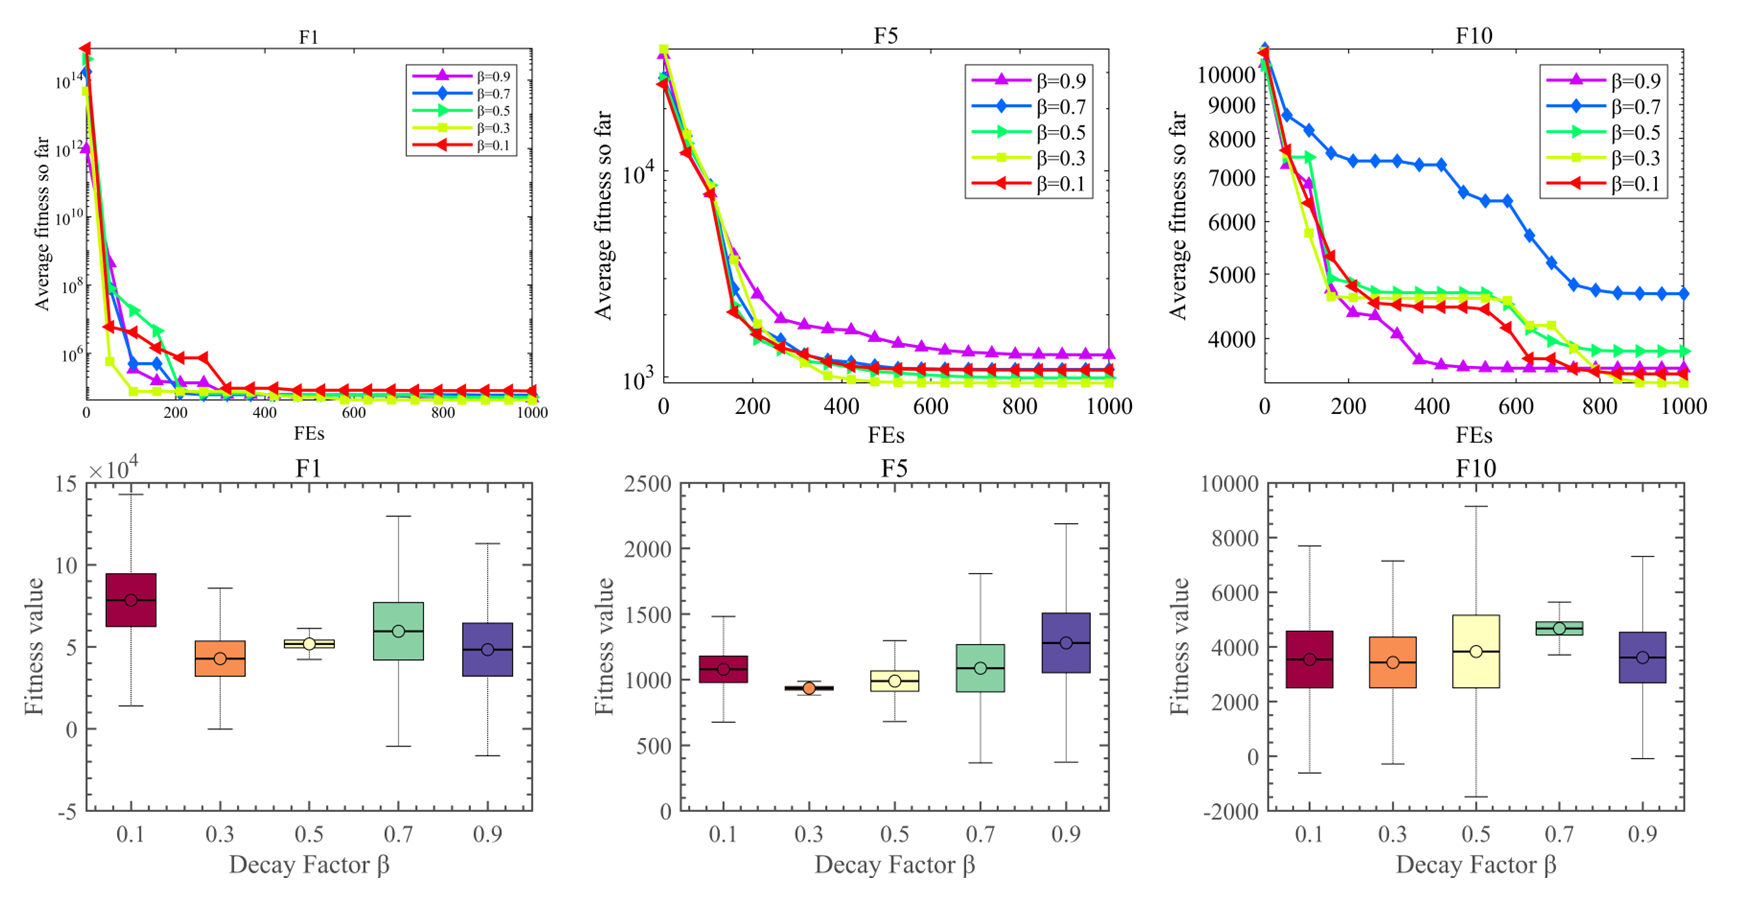
\includegraphics[width=\textwidth]{figures/chapter5/beta.png}
    \bicaption{不同$\beta$设置下BEXEA的性能}{Performance of BEXEA under different $\beta$ settings}
    \label{fig:bexea_Beta}
\end{figure}

\begin{figure}
    \centering
    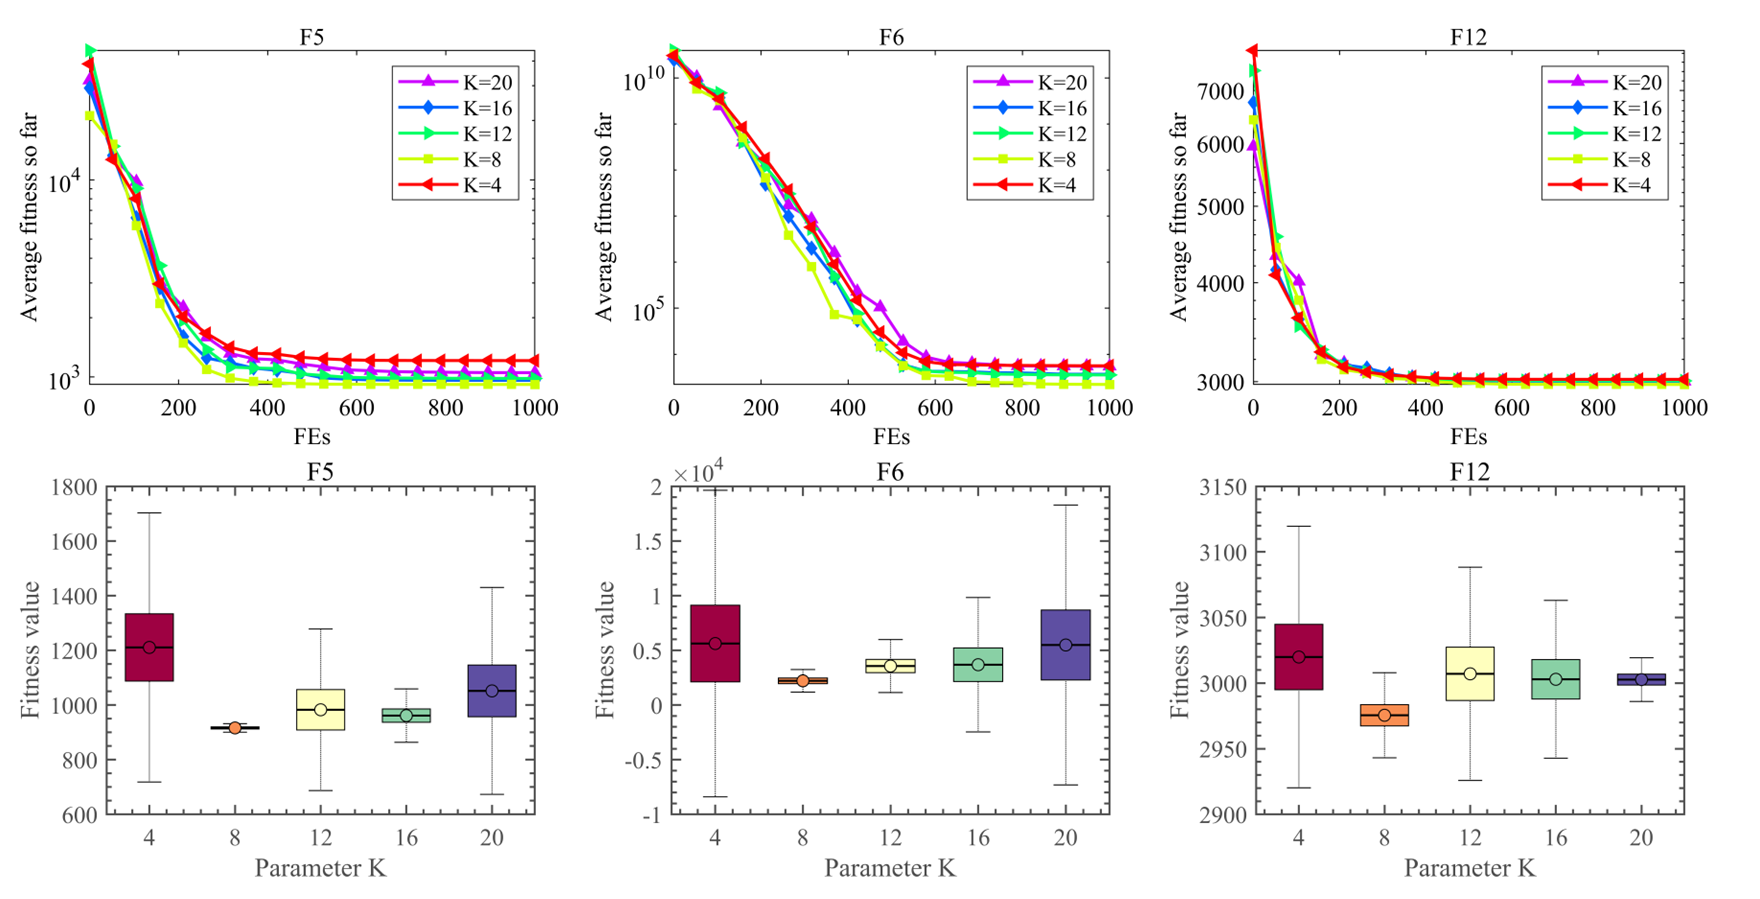
\includegraphics[width=\textwidth]{figures/chapter5/k.png}
    \bicaption{不同$\mathcal{K}$设置下BEXEA的性能}{Performance of BEXEA under different $\mathcal{K}$ settings}
    \label{fig:bexea_K}
\end{figure}

\subsubsection{油藏产量优化实验}

本项实验采用了MRST工具箱构建仿真环境，针对复杂的井控问题进行实测。

\begin{table}[htbp]
\bicaption{BEXEA与其他SAEAs在油藏产量优化问题上的比较结果}{Comparison results of BEXEA and other SAEAs on the oil reservoir production optimization problem}
\label{t:bexea_Oil_Exp_Table}
\resizebox{\textwidth}{!}{
\begin{tabular}{lcccc}
\toprule
Algorithm & Avg(std)                    & Worst             & Best              & Running time      \\
\midrule
TSABFEA   & 7.7893E+07(1.63E+05)          & 7.7567E+07          & 7.8219E+07          & 3.4710E+04          \\
KTA2      & 7.7750E+07(7.01E+05)          & 7.6348E+07          & 7.9152E+07          & 4.6481E+04          \\
DESO      & 7.6402E+07(7.53E+05)          & 7.4896E+07          & 7.7908E+07          & 2.8266E+04          \\
MS\_MTO   & 7.9145E+07(3.76E+05)          & 7.8393E+07          & 7.9897E+07          & 2.4439E+04          \\
ESA       & 7.6279E+07(6.18E+05)          & 7.5043E+07          & 7.7515E+07          & 2.5137E+04          \\
ToSADE    & 7.8500E+07(6.34E+05)          & 7.7232E+07          & 7.9768E+07          & 2.5435E+04          \\
SHPSO     & 7.6296E+07(3.42E+05)          & 7.5612E+07          & 7.6980E+07          & 2.3522E+04          \\
BEXEA     & \textbf{7.9995E+07(1.12E+05)} & \textbf{7.9771E+07} & \textbf{8.0219E+07} & \textbf{2.1334E+04}\\
\bottomrule
\end{tabular}}
\end{table}

表\ref{t:bexea_Oil_Exp_Table}的结果显示，BEXEA在所有核心经济指标上均优于竞争算法。其平均NPV不仅较次优算法提升了逾百万美元，且在结果的一致性（标准差）与运行效率方面也展现出明显优势。这种高效性对于需要频繁执行高保真模拟的石油工程决策而言，具有极高的实用价值。

\begin{figure}
    \centering
    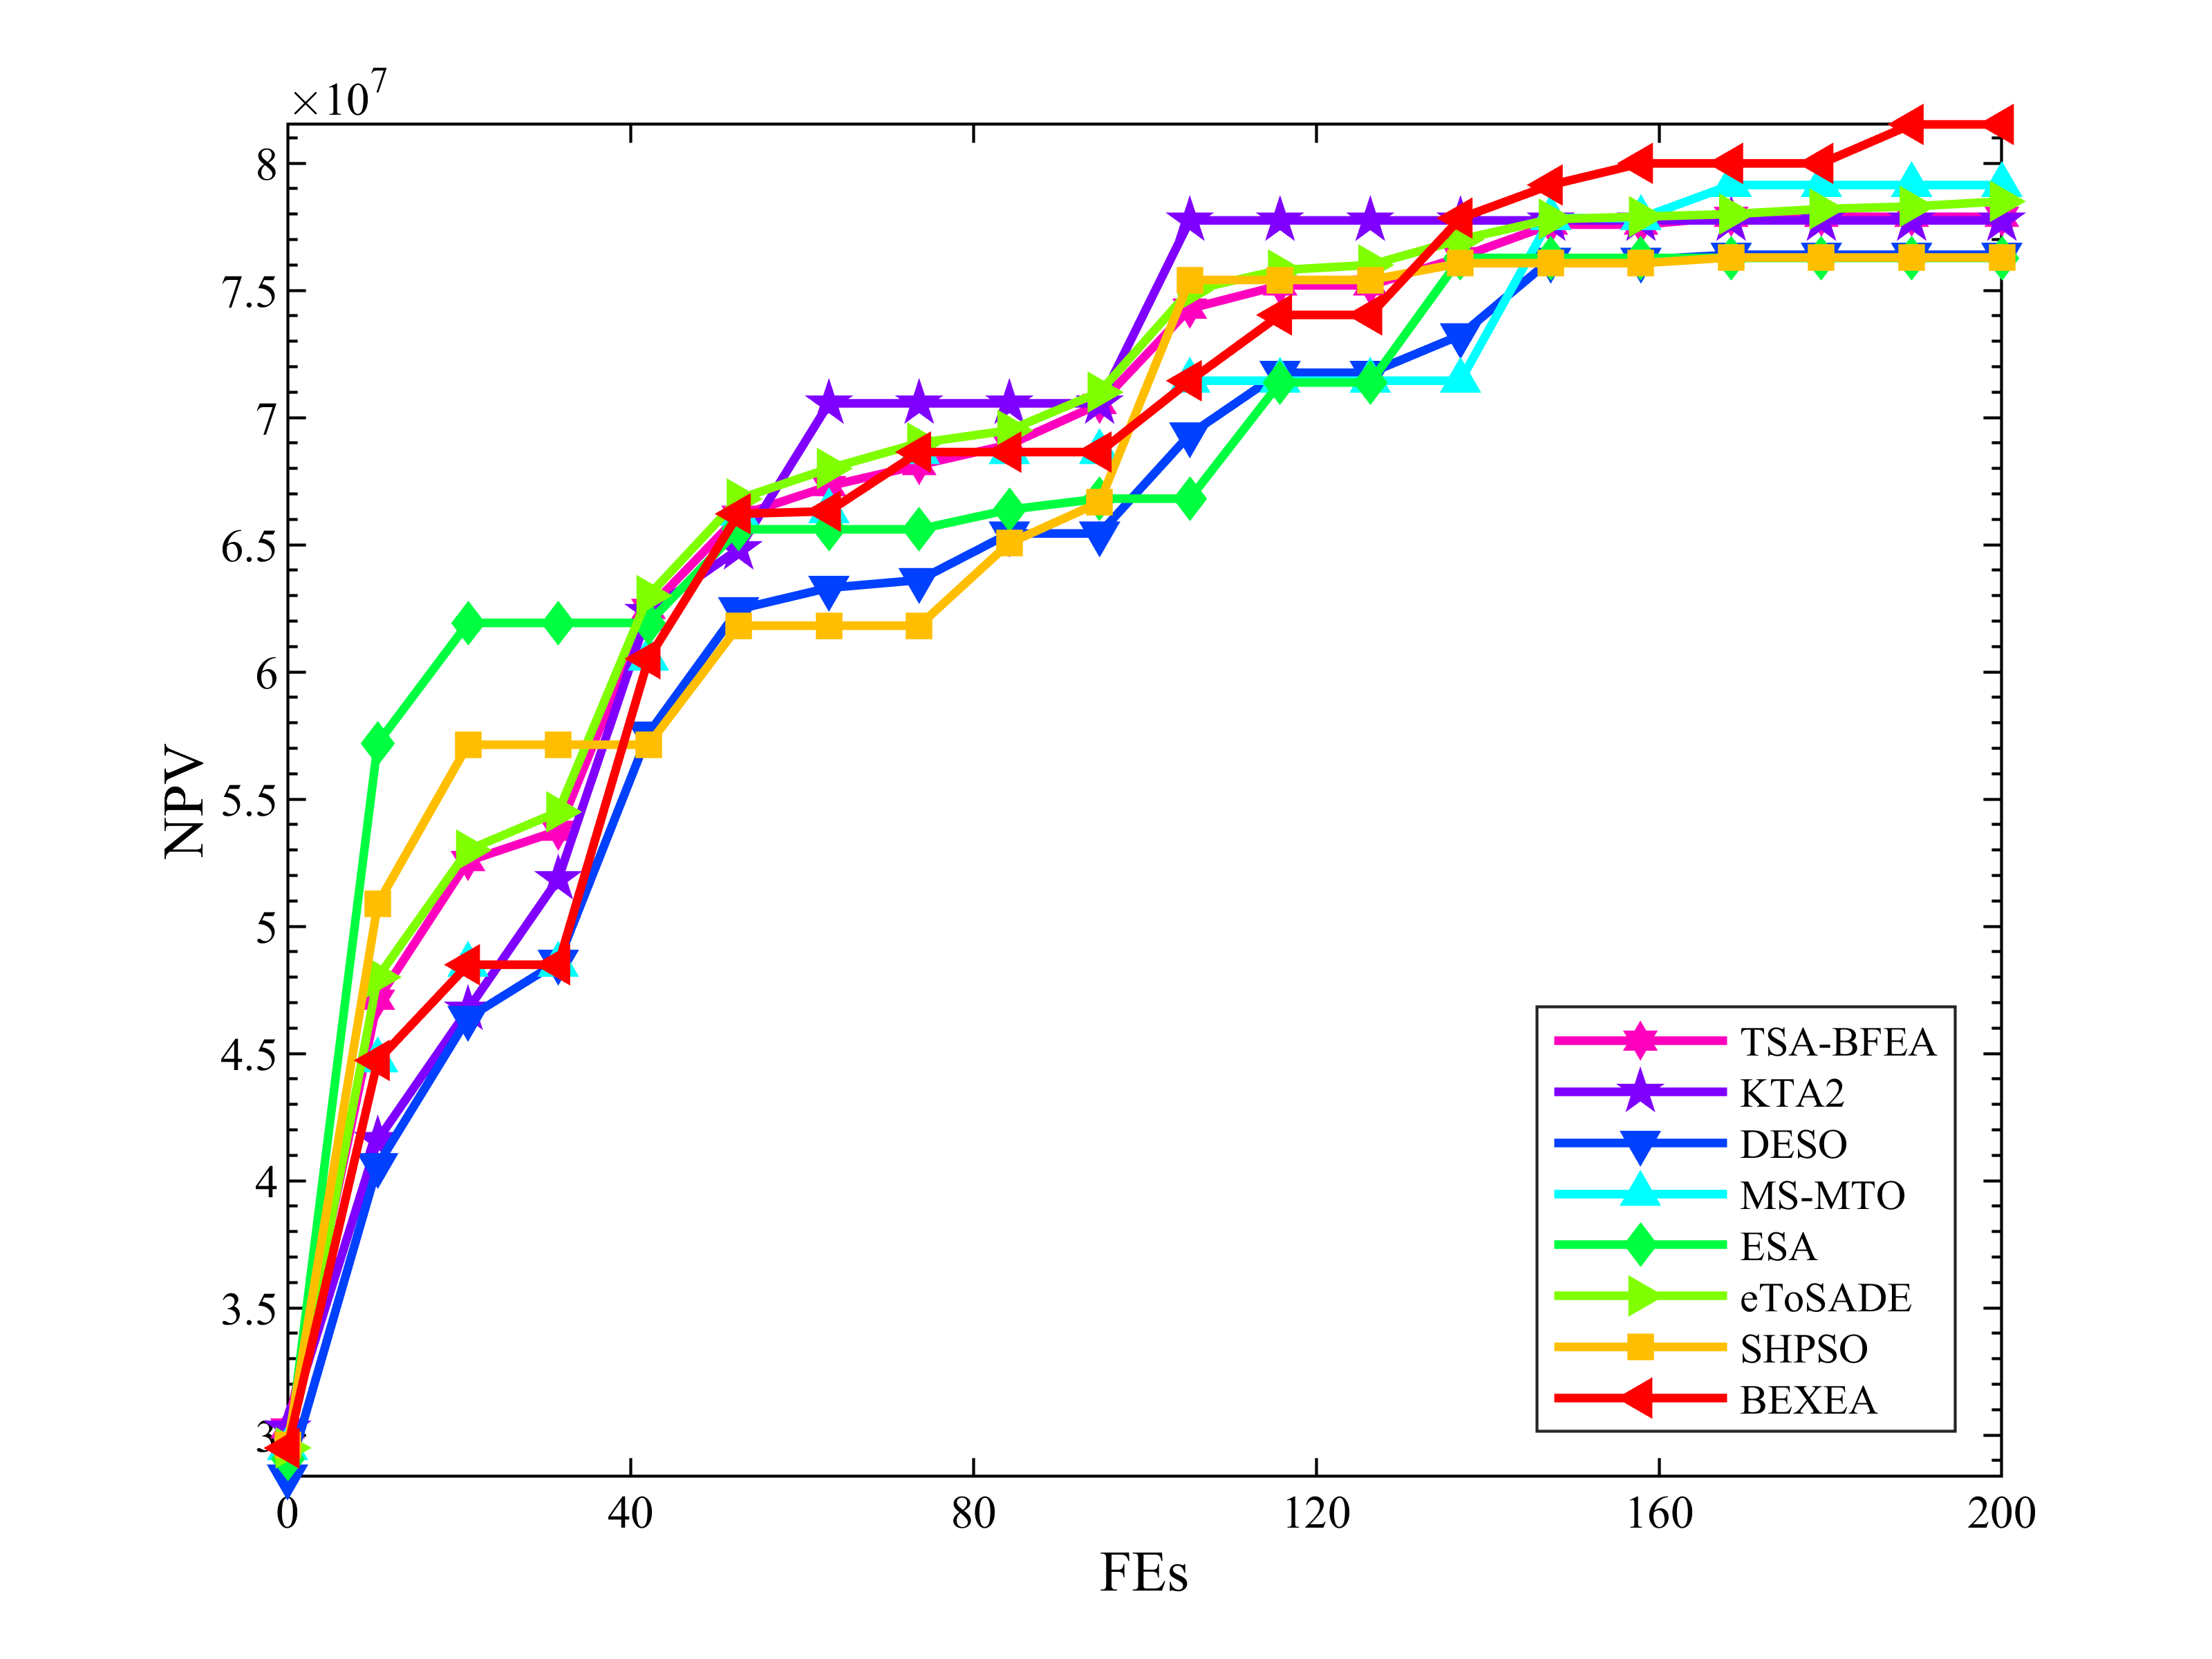
\includegraphics[width=\textwidth]{figures/chapter5/runBEXEA-OilReservoir-sampled-CC.png}
    \bicaption{BEXEA与其他SAEAs在油藏产量优化问题上的收敛曲线}{Convergence curves of BEXEA and other SAEAs on the oil reservoir production optimization problem}
    \label{fig:bexea_Oil_Exp_Figure}
\end{figure}

图\ref{fig:bexea_Oil_Exp_Figure}刻画的收敛轨迹展示了BEXEA极佳的起步能力。在优化的中后期，得益于MAB机制对搜索陷入停滞的敏锐捕捉与及时调整，算法能持续保持向更优解靠拢的势头，最终在受限的评估预算内取得了最佳经济收益。

\section{本章小结}
本章针对代理辅助昂贵优化中普遍存在的策略僵化与采样准则黑箱化问题，研发了BEXEA算法。该方法通过融合多臂赌博机的自适应搜索与可解释人工智能技术，实现了对搜索资源与采样决策的智能化协同管理。

全方位的实验验证表明，BEXEA在不同维度的标准测试套件上均展现了超越同类先进算法的优化能力。其在油藏工程实测算例中的成功应用，进一步印证了该方法在处理真实复杂昂贵问题时的优越样本效率与实战价值。消融实验的数据也充分解构了自适应切换与多准则采样对算法性能提升的具体贡献。整体而言，BEXEA在减少对人工先验设计依赖的同时，提升了优化决策的透明度，为昂贵优化问题的求解提供了一种更高效且具解释性的新路径。


%%% Chapter 6: 总结与展望 (Conclusion and Outlook)
% Chapter 6: 总结与展望 (Conclusion and Outlook)
\chapter{总结与展望}

\section{本文工作总结}
% TODO: 总结全文的主要研究工作和创新点

\subsection{IBSA算法研究总结}
% TODO: 总结第三章IBSA的主要贡献
% - 精英引导变异策略
% - CEC 2017基准测试中的表现
% - bIBSA在特征选择中的应用

\subsection{SBO算法研究总结}
% TODO: 总结第四章SBO的主要贡献
% - 基于状态的优化机制
% - 连续优化、特征选择和图像分割中的表现

\subsection{BEXEA算法研究总结}
% TODO: 总结第五章BEXEA的主要贡献
% - 赌博机驱动的自适应搜索策略
% - 可解释的不确定性准则
% - 代理辅助优化中的表现

\section{研究展望}
% TODO: 讨论未来的研究方向
% - 高维空间中的算法性能
% - 更多实际工程问题的应用
% - 算法的理论分析
% - 多目标优化的扩展
% - 深度学习与元启发式算法的结合


\newpage

\backmatter
\renewcommand{\chaptermark}[1]{\markboth{\songti #1}{}}
\makereferences
\newpage



{
    \appendix
    \renewcommand{\chaptermark}[1]{\markboth{\heiti  附录\thechapter\ ~#1}{}}
    \chapter{补充材料}

    % TODO: 添加附录内容，例如SBO论文的补充实验数据表格
    \section{补充实验数据}
    本附录包含各章节实验的补充数据和详细结果。

    \newclearpage
}
\ifdefined\blind  %这个if不要删除
    % 盲审版没有致谢
\else
    \chapter{致谢}

    % TODO: 填写致谢内容
    致谢内容待填写。

    \vskip 108pt
    \begin{flushright}
        王健\makebox[1cm]{} \\
        \today
    \end{flushright}
    \newpage
\fi
\chapter{攻读硕士学位期间取得的主要学术成果}

\section*{1. 已发表的学术论文}
% TODO: 填写已发表的学术论文

\ifdefined\blind  % 这个if不要删除
    % 盲审版不透露自己姓名
    \begin{enumerate}
        \renewcommand{\labelenumi}{[\arabic{enumi}]}
        \setlength{\itemindent}{0em}
        \setlength{\labelsep}{0.5em}

        \item The Status-based Optimization: Algorithm and Comprehensive Performance Analysis[J]. Neurocomputing. SCI收录，已录用，第四章的研究成果.
        \item Elite Leading Mutation Backtracking Search Algorithm for High-Dimensional Medical Data Feature Selection[J]. 审稿中，第三章的研究成果.
        \item Bandit-Driven Adaptive Search in Surrogate-Assisted Evolutionary Algorithm with Explainable Uncertainty Criteria[J]. 审稿中，第五章的研究成果.
    \end{enumerate}
\else
    \begin{enumerate}
        \renewcommand{\labelenumi}{[\arabic{enumi}]}
        \setlength{\itemindent}{0em}
        \setlength{\labelsep}{0.5em}

        \item Wang J, Chen Y, Lu C, Heidari A A, Wu Z, Chen H. The Status-based Optimization: Algorithm and Comprehensive Performance Analysis[J]. Neurocomputing. SCI收录，已录用，第四章的研究成果.
        \item Wang J, Chen Y, Zou H, Lu C, Heidari A A, Liu L, Chen H, Liang G. Elite Leading Mutation Backtracking Search Algorithm for High-Dimensional Medical Data Feature Selection[J]. 审稿中，第三章的研究成果.
        \item Wang J, Chen Y, Lu C, Heidari A A, Liu L, Chen H. Bandit-Driven Adaptive Search in Surrogate-Assisted Evolutionary Algorithm with Explainable Uncertainty Criteria[J]. 审稿中，第五章的研究成果.
    \end{enumerate}
\fi

\section*{2. 知识产权}

\begin{enumerate}
    \renewcommand{\labelenumi}{[\arabic{enumi}]}
    \setlength{\itemindent}{0em}
    \setlength{\labelsep}{0.5em}

    \item 发明专利：一种多阈值图像分割方法、装置、计算机设备及存储介质，申请号：2025110129939，第2发明人，已授权.
\end{enumerate}

\section*{3. 获奖情况}

\begin{enumerate}
    \renewcommand{\labelenumi}{[\arabic{enumi}]}
    \setlength{\itemindent}{0em}
    \setlength{\labelsep}{0.5em}

    \item 国家级铜奖（团队排名3/15），第十四届"挑战杯"中国大学生创业计划竞赛"一带一路"国际邀请赛，2024年.
    \item 省级银奖（团队负责人），"建行杯"浙江省国际大学生创新大赛，2024年.
    \item 校级金奖（团队排名4/15），温州大学第十一届"挑战杯"竞赛，2025年.
    \item 温州大学一等奖学金，2024年.
\end{enumerate}

%\newpage
\end{document}
